\documentclass[12pt]{article}
%\documentclass{jarticle}
%\pagestyle{empty}                      % <======= surpress page numbers
\newcommand{\bld}[1]{\mbox{\boldmath $#1$}}
\newcommand{\utilde}[1]{\mbox{$#1$}\hspace{-.8em}\raisebox{-1ex}{$\sim$}}
\newcommand{\leftdef}[0]{\,\mbox{$\stackrel{\leftarrow}{=}$}\,}
\newcommand{\rightdef}[0]{\,\mbox{$\stackrel{\rightarrow}{=}$}\,}
\newcommand{\bra}[0]{<\!}
\newcommand{\braketend}[0]{\,|\,}
\newcommand{\braend}[0]{|\,}
\newcommand{\ketend}[0]{\,|}
\newcommand{\ket}[0]{\!>}
\newcommand{\ctext}[1]{\raise0.2ex\hbox{\textcircled{\scriptsize{#1}}}}
\newcommand{\maru}[1]{\ooalign{
\hfil\resizebox{.8\width}{\height}{\scriptsize{#1}}\hfil
\crcr
\raise0.2ex\hbox{\large$\bigcirc$}}}
\newcommand{\normord}[1]{%
  {:\mathrel{\mspace{1mu}#1\mspace{1mu}}:}%
}
\newcommand{\normalprod}[1]{%
  {:\mathrel{\mspace{1mu}#1\mspace{1mu}}:}%
}


%--------------------------   Source Directories ---------------
\newcommand{\myqftsrcdirectory}[0]{myqft/src}
%\newcommand{\mainsrcdirectory}[0]{../src}
\newcommand{\mainqftsrcdirectory}[0]{src_qft}
%\newcommand{\mfdirectory}[0]{../src/mfonts}
\newcommand{\feynmfdirectory}[0]{feynmf}
\newcommand{\srcseventeen}[0]{myqft/versions/2017}
\newcommand{\myphotondirectory}[0]{myqft/versions/2017photon} % this directory should be absorbed somewhere


%\oddsidemargin 10pt
%\evensidemargin 10pt
\setlength{\textheight}{42\baselineskip}
%\textheight 600pt
\topmargin -5mm
\footskip 25mm
 \renewcommand\footnoterule{
 %\vspace*{-3pt}%
 \vspace*{9pt}%
     \hrule width 2in height 0.4pt
     \vspace*{2.6pt}}
%\marginparsep 5cm
%\marginparwidth5cm

\newcounter{exercise}

\newcounter{problem}
\newcounter{refprob}
%080219 Problems are numbered by a new counter "problem".
%       One additional counter "refprob" is defined to refer
%       to a previous problem. Find an example in
%       set07/sec02F_3dim_x.tex
%\oddsidemargin10pt
\newcounter{exple}
\newcounter{refexple}
%100104 Examples are numbered by a new counter "exple".
%       One additional counter "refexple" is defined to refer
%       to a previous example. 

\usepackage{cite}

\usepackage{graphicx}
\usepackage{latexsym}
\usepackage{amssymb}
\usepackage{ulem}
\usepackage{cancel}
\usepackage{comment}
%\usepackage{multicol}
%\setlength{\columnseprule}{1pt}
%\usepackage{vwcol}
\usepackage{amsmath}
\DeclareMathOperator{\tr}{tr}
\usepackage{arydshln}  %dashed line in a matrix

\usepackage{feynmp}%%%{feynmp}

\usepackage{color}
\newcommand{\bl}[0]{\color{blue}}
\newcommand{\re}[0]{\color{red}}
\newcommand{\gr}[0]{\color{green}}
\newcommand{\cy}[0]{\color{cyan}}
\newcommand{\ma}[0]{\color{magenta}}
\newcommand{\ye}[0]{\color{yellow}}

\include{hugenholtz}  % macros for hugenholtz diagrams

\usepackage{slashed}

\usepackage[vcentermath]{youngtab}
\usepackage{simplewick}

\usepackage{enumitem} % ToDo list
\newlist{todolist}{itemize}{2}
\setlist[todolist]{label=$\square$}
\usepackage{pifont}
\newcommand{\cmark}{\ding{51}}
\newcommand{\done}{\rlap{$\square$}{\raisebox{2pt}{\large\hspace{1pt}\cmark}}%
\hspace{-2.5pt}}

\begin{document}

\begin{titlepage} 
\vspace*{3cm}
\vspace*{2cm}
\noindent
\begin{center}
{\Huge \bf An Introduction to Relativistic Quantum Field Theory\\}  
%--private:  {\Huge \bf Private Notes on Relativistic Quantum Field Theory\\}  
\vspace{1cm}
{\large Year 2018}
\vspace{1cm}
\\
{\Large 
Schin Dat\'e}
\end{center}
\end{titlepage} 


\pagenumbering{gobble}

\tableofcontents
%==================

\thispagestyle{empty}

\pagenumbering{arabic}
%\pagenumbering{roman}


\setcounter{page}{0}
%\setcounter{section}{-1}
%\setcounter{page}{0}
\setcounter{section}{-1}

\newpage % to keep a space for the contents

%========================================  Notations
%\begin{center}
%{\bf \Large Notations}
%\end{center}
\section{Notations}
%\thispagestyle{empty}

%%\setcounter{subsection}{-1}
%\subsection{Notations}
$\blacksquare$
metric of 4-vector space:
\begin{equation*}
   g = 
 \left( \begin{array}{cccc}
       1 & 0&0&0\\
       0 & -1&0&0\\
       0 & 0&-1&0\\
       0 & 0&0&-1\\
              \end{array} \right)\hspace{10mm}({\mbox{\small "Bjorken-Drell metric"}})
\label{eqn:metric}
\end{equation*}
The square of a 4-vector $\underline{p} = (p^0, \bld{p}) = (p^0, p^1, p^2, p^3)$ is
\[ \underline{p}^2 = \underline{p}^T g\, \underline{p} = (p^0)^2 - (p^1)^2 - (p^2)^2 - (p^3)^2 = (p^0)^2 - \bld{p}^2\,, \]
where a superscript $T$ denotes the transpose. An underline on a quantity (e.g. $\underline{p}$) indicates a 
%contravariant 
4-vector but it is frequently suppressed.
% and $\underline{p}$ is written just as $p$, when there is no possibility of confusions.
When components of a 4-vector are given, they are contravariant components by default.
The contravariant components of a 4-vector $\underline{p}$ are denoted as $p^{\mu}$ with
upper suffixes. To make sure that components are contravariant, we often denote a 4-vector
itself as $p^{\mu}$. For given contravariant components, covariant components are obtained
as
\[ p_{\mu} = g_{\mu \nu} p^\nu \,,\]
where $g_{\mu \nu}$ is the ($\mu \nu$) element of $g$.
Thus, for the $\underline{p}$ given in the above, we write $p_{\mu} = (p^0, -\bld{p})$.
The square of a 4-vector $\underline{p}$ is now also written as
\[ \underline{p}^2 = p_{\mu} p^{\mu} \,,\]
where same suffixes $\mu$ in lower and upper positions must be summed over $\mu \in [0,3]$.

\bigskip

\bigskip


\noindent
$\blacksquare$ Energy-momentum of a particle of the mass $m$ is written as
\begin{equation*}
	p^\mu \;\leftdef
         \left( \begin{array}{c} E/ c \\ 
          \bld{p}  \end{array} \right)  
          =
	mc
         \left( \begin{array}{c} \gamma \\ 
          \gamma\bld{\beta}  \end{array} \right)  
          = m u^\mu \,,
\label{eqn:enmomvec}
\end{equation*}
where $\gamma \equiv 1 /\sqrt{1 - \bld{\beta}^2}$ denotes the Lorentz factor of motion of the particle,
$\bld{\beta}$ stands for the velocity nomalized by one of the light, $c$,
and $u^\mu$ is the four-velocity.

\bigskip

\bigskip


\noindent
$\blacksquare$ Natural unit ($c = \hbar = 1$) is employed throughout our discussions.
E.g. for the energy-momentum given in the above, we write
\[ E = \sqrt{\bld{p}^2 + m^2} 
\hspace{3mm}
\mbox{and}
\hspace{3mm}
\underline{p}^2 = m^2 \,.
\]

\noindent
$\blacksquare$
Nomalization of states\\
\begin{equation*}
\begin{array}{l}
\mbox{Energy-momentum eigenstate:}\hspace{3mm}
 \bra p \braketend p' \ket = 2 E \delta^3 ( \bld{p} - \bld{p}' )$,\hspace{2mm}$E = \sqrt{m^2 + \bld{p}^2}\\
\mbox{Completeness:}\hspace{3mm}
{\displaystyle   \int \frac{d^3 \bld{p}}{2E}} \ketend p \ket \bra p \braend = 1\,.
\end{array}
\label{eqn:statenormalization}
\end{equation*}
Many authors including ones of Refs. \cite{ref:Donnachie} and \cite{ref:Collins} 
put a factor $(2\pi)^3$ in the front of $\delta$ function and in the denominator 
of the integration volume element. It is just a matter of convention.
Note that
\begin{equation*}
Dim[ \ketend p \ket ] = [E] ^{-1}
\end{equation*}

\noindent
$\blacksquare$
Levi-Civita symbols\\
These are totally antisymmetric tensor densities.\\

\noindent
3 dimensional
\begin{eqnarray*}
\epsilon_{ijk}
=
\left\{
\begin{array}{l}
\raisebox{-.3\height}{${\stackrel{\displaystyle+}{-}}$} \;1
\hspace{5mm}
(i, j, k) =
\raisebox{-.3\height}{$\stackrel{\mbox{even}}{\mbox{odd}}$} \,\;\mbox{permutation of } (1,2,3)
\vspace{2mm}
\\
0
\hspace{5mm}
\mbox{otherwise}
\end{array}
\right.
\label{eqn:LeviCivita3dim}
\end{eqnarray*}
For the purpose of applying the Einstein's contraction rule to 3 vector suffices,
we may use symbols like $\epsilon^{ijk}$, $\epsilon_{ij}^{\;\;\;k}$ and so on.
All these symbols are equivalent with $\epsilon_{ijk}$.
%Eq. (\ref{eqn:LeviCivita3dim}).
The vertical positions of indexes have no meaning.\\

\noindent
4 dimensional
\begin{eqnarray*}
\epsilon^{\mu\nu\rho\sigma}
=
\left\{
\begin{array}{l}
+ 1
\hspace{5mm}
(\mu, \nu, \rho, \sigma, ) = \mbox{even parmutation of } (0, 1, 2, 3)
\\
- 1
\hspace{5mm}
(\mu, \nu, \rho, \sigma, ) = \mbox{odd parmutation of } (0, 1, 2, 3)
\\
0
\hspace{5mm}
\mbox{otherwise}
\end{array}
\right.
\end{eqnarray*}
Symbols with covariant suffices are defined with the metric tensor 
in such a way like $\epsilon_\mu^{\;\;\nu\rho\sigma} = g_{\mu \tau} \epsilon^{\tau \nu\rho\sigma}$.
Therefore, we have $\epsilon_{\mu\nu\rho\sigma} = - \epsilon^{\mu\nu\rho\sigma}$.
This notation follows \cite{ref:Peskin-Schroeder}.

%\setcounter{subsection}{-1}
%\subsection{Notations}
$\blacksquare$
metric of 4-vector space:
\begin{equation*}
   g = 
 \left( \begin{array}{cccc}
       1 & 0&0&0\\
       0 & -1&0&0\\
       0 & 0&-1&0\\
       0 & 0&0&-1\\
              \end{array} \right)\hspace{10mm}({\mbox{\small "Bjorken-Drell metric"}})
\label{eqn:metric}
\end{equation*}
The square of a 4-vector $\underline{p} = (p^0, \bld{p}) = (p^0, p^1, p^2, p^3)$ is
\[ \underline{p}^2 = \underline{p}^T g\, \underline{p} = (p^0)^2 - (p^1)^2 - (p^2)^2 - (p^3)^2 = (p^0)^2 - \bld{p}^2\,, \]
where a superscript $T$ denotes the transpose. An underline on a quantity (e.g. $\underline{p}$) indicates a 
%contravariant 
4-vector but it is frequently suppressed.
% and $\underline{p}$ is written just as $p$, when there is no possibility of confusions.
When components of a 4-vector are given, they are contravariant components by default.
The contravariant components of a 4-vector $\underline{p}$ are denoted as $p^{\mu}$ with
upper suffixes. To make sure that components are contravariant, we often denote a 4-vector
itself as $p^{\mu}$. For given contravariant components, covariant components are obtained
as
\[ p_{\mu} = g_{\mu \nu} p^\nu \,,\]
where $g_{\mu \nu}$ is the ($\mu \nu$) element of $g$.
Thus, for the $\underline{p}$ given in the above, we write $p_{\mu} = (p^0, -\bld{p})$.
The square of a 4-vector $\underline{p}$ is now also written as
\[ \underline{p}^2 = p_{\mu} p^{\mu} \,,\]
where same suffixes $\mu$ in lower and upper positions must be summed over $\mu \in [0,3]$.

\bigskip

\bigskip


\noindent
$\blacksquare$ Energy-momentum of a particle of the mass $m$ is written as
\begin{equation*}
	p^\mu \;\leftdef
         \left( \begin{array}{c} E/ c \\ 
          \bld{p}  \end{array} \right)  
          =
	mc
         \left( \begin{array}{c} \gamma \\ 
          \gamma\bld{\beta}  \end{array} \right)  
          = m u^\mu \,,
\label{eqn:enmomvec}
\end{equation*}
where $\gamma \equiv 1 /\sqrt{1 - \bld{\beta}^2}$ denotes the Lorentz factor of motion of the particle,
$\bld{\beta}$ stands for the velocity nomalized by one of the light, $c$,
and $u^\mu$ is the four-velocity.

\bigskip

\bigskip


\noindent
$\blacksquare$ Natural unit ($c = \hbar = 1$) is employed throughout our discussions.
E.g. for the energy-momentum given in the above, we write
\[ E = \sqrt{\bld{p}^2 + m^2} 
\hspace{3mm}
\mbox{and}
\hspace{3mm}
\underline{p}^2 = m^2 \,.
\]

\noindent
$\blacksquare$
Nomalization of states\\
\begin{equation*}
\begin{array}{l}
\mbox{Energy-momentum eigenstate:}\hspace{3mm}
 \bra p \braketend p' \ket = 2 E \delta^3 ( \bld{p} - \bld{p}' )$,\hspace{2mm}$E = \sqrt{m^2 + \bld{p}^2}\\
\mbox{Completeness:}\hspace{3mm}
{\displaystyle   \int \frac{d^3 \bld{p}}{2E}} \ketend p \ket \bra p \braend = 1\,.
\end{array}
\label{eqn:statenormalization}
\end{equation*}
Many authors including ones of Refs. \cite{ref:Donnachie} and \cite{ref:Collins} 
put a factor $(2\pi)^3$ in the front of $\delta$ function and in the denominator 
of the integration volume element. It is just a matter of convention.
Note that
\begin{equation*}
Dim[ \ketend p \ket ] = [E] ^{-1}
\end{equation*}

\noindent
$\blacksquare$
Levi-Civita symbols\\
These are totally antisymmetric tensor densities.\\

\noindent
3 dimensional
\begin{eqnarray*}
\epsilon_{ijk}
=
\left\{
\begin{array}{l}
\raisebox{-.3\height}{${\stackrel{\displaystyle+}{-}}$} \;1
\hspace{5mm}
(i, j, k) =
\raisebox{-.3\height}{$\stackrel{\mbox{even}}{\mbox{odd}}$} \,\;\mbox{permutation of } (1,2,3)
\vspace{2mm}
\\
0
\hspace{5mm}
\mbox{otherwise}
\end{array}
\right.
\label{eqn:LeviCivita3dim}
\end{eqnarray*}
For the purpose of applying the Einstein's contraction rule to 3 vector suffices,
we may use symbols like $\epsilon^{ijk}$, $\epsilon_{ij}^{\;\;\;k}$ and so on.
All these symbols are equivalent with $\epsilon_{ijk}$.
%Eq. (\ref{eqn:LeviCivita3dim}).
The vertical positions of indexes have no meaning.\\

\noindent
4 dimensional
\begin{eqnarray*}
\epsilon^{\mu\nu\rho\sigma}
=
\left\{
\begin{array}{l}
+ 1
\hspace{5mm}
(\mu, \nu, \rho, \sigma, ) = \mbox{even parmutation of } (0, 1, 2, 3)
\\
- 1
\hspace{5mm}
(\mu, \nu, \rho, \sigma, ) = \mbox{odd parmutation of } (0, 1, 2, 3)
\\
0
\hspace{5mm}
\mbox{otherwise}
\end{array}
\right.
\end{eqnarray*}
Symbols with covariant suffices are defined with the metric tensor 
in such a way like $\epsilon_\mu^{\;\;\nu\rho\sigma} = g_{\mu \tau} \epsilon^{\tau \nu\rho\sigma}$.
Therefore, we have $\epsilon_{\mu\nu\rho\sigma} = - \epsilon^{\mu\nu\rho\sigma}$.
This notation follows \cite{ref:Peskin-Schroeder}.


%}
\setcounter{footnote}{0}
\setcounter{equation}{0}
\setcounter{figure}{0}
\setcounter{problem}{0}

\newpage
%============================================== section Starting, Noether
%\part{Introduction}
\section{Starting from Quantum Mechanics}
\subsection{Basic matters}
%Operators acting in a Hilbert space. Physical quantities are hermitian operators.
%Born's probability interpretation is employed.\\
\begin{eqnarray}
\mbox{Schr\"odinger eq.} \hspace{24mm} 
&\hspace{-5mm}&
\hspace{-20mm}
i \partial_t \Psi(t, \bld{x}) = {H} \Psi(t, \bld{x}) \,,
%i \partilal_t \Psi (t, \bld{x}) = H \Psi (t, \bld{x})
\hspace{3mm}
H = - \frac{\bld{\partial}^2}{2m} + V(\bld{x}) = H^\dagger
\label{eqn:SchroedingerEq}
\\
\mbox{Eigenstates of } H \hspace{22mm} 
&\hspace{-5mm}&
\hspace{-20mm}
H \varphi_l (\bld{x} ) = \epsilon_l \varphi_l (\bld{x} )\,,
\hspace{3mm}
\{ \varphi_l (\bld{x} ) \} \mbox{: orthogonal, complete}
\label{eqn:energyEigenSt}
\\
\mbox{Solution of the Schr\"odinger eq.}
&\hspace{-5mm}&
\Psi(t, \bld{x})
=
\sum_l \Psi_l e^{-i \epsilon_l t} \varphi_l (\bld{x})
\label{eqn:Psiexpansion}
\end{eqnarray}
%-------------------------------------------------------------------
%
Bras and kets
\begin{equation}
\Psi(t, \bld{x}) = \bra \bld{x} \braend \Psi(t) \ket\,,
\hspace{5mm}
\varphi_l(\bld{x})  = \bra \bld{x} \braend \epsilon_l \ket\,, 
\label{eqn:coordrepbraket}
\end{equation}
\begin{equation*}
\hspace{21mm}
i \partial_t  \ketend \Psi(t) \ket = \hat{H} \ketend \Psi(t) \ket\,,
\hspace{5mm}
\hat{H} = \frac{\hat{\bld{p}}^2}{2 m} + V(\bld{x}) = \hat{H}^\dagger
\hspace{20mm}
\bra \ref{eqn:SchroedingerEq} \ket
\end{equation*}
\begin{equation*}
\hspace{13mm}
\hat{H} 
\ketend \epsilon_l \ket
= 
\epsilon_l \ketend \epsilon_l \ket\,,
\hspace{3mm}
\bra \epsilon_l \ketend \epsilon_{l'} \ket = 0 \mbox{ if } l\neq l'\,,
\hspace{3mm}
\sum_l \ketend \epsilon_{l} \ket \bra \epsilon_{l} \braend = 1
\hspace{10mm}
\bra \ref{eqn:energyEigenSt} \ket
\end{equation*}
\begin{equation*}
\hspace{32mm}
\ketend \Psi(t) \ket =
\sum_l \bra \epsilon_l \braend   \Psi(0) \ket
e^{-i \epsilon_l t} \ketend \epsilon_l \ket
\hspace{30mm}
\bra \ref{eqn:Psiexpansion} \ket
\end{equation*}
%-------------------------------------------------------------------
%
1st quantization
\begin{equation}
[\hat{x}_i, \hat{p}_j] = i \delta_{ij}
\end{equation}
Eigen states
\begin{equation}
\begin{array}{l}
\hat{\bld{x}} \ketend \bld{x} \ket = \bld{x} \ketend \bld{x} \ket
\\
\hat{\bld{p}} \ketend \bld{p} \ket = \bld{p} \ketend \bld{p} \ket
\end{array}
\end{equation}
Conventional ("half relativistic") normalization
\begin{equation}
\bra \bld{x} \braend \bld{x}' \ket = \delta^3(\bld{x}-\bld{x}')\,,
\hspace{5mm}
\int \ketend \bld{x} \ket d^3 \bld{x} \bra \bld{x} \braend = 1
\end{equation}
\begin{equation}
\bra \bld{p} \braend \bld{p}' \ket = 2E \delta^3(\bld{p}-\bld{p}')\,,
\hspace{5mm}
\int \ketend \bld{p} \ket \frac{d^3 \bld{p}}{2E} \bra \bld{p} \braend = 1
\label{eqn:norm_p_state_rel}
\end{equation}
Coordinate representation of the momentum operator
\begin{equation}
\bra \bld{x} \braend \hat{\bld{p}}
=
\frac{1}{i} \bld{\partial} \bra \bld{x} \braend
\end{equation}
and of the momentum eigenstate
\begin{equation}
\bra \bld{x} \braend \bld{p} \ket
=
\sqrt{\frac{2E}{(2\pi)^3}}\, e^{i \bld{p} \cdot \bld{x}}
\end{equation}
Requirement for the normalization factor is understood by employing
the first equation of (\ref{eqn:norm_p_state_rel}) in the $l.h.s$ of
$\nolinebreak{\bra \bld{p} \braend \bld{p}' \ket}= $
$\nolinebreak{\int \bra \bld{p} \braend \bld{x} \ket d^3\bld{x} \bra \bld{x} \ketend \bld{p}' \ket}$
and remembering a formula
\[
\int {d^3 \bld{x}}\, e^{\pm i \bld{p} \cdot \bld{x}}= (2\pi)^3 \delta^3 (\bld{p})
\]

\subsection{$N$-body quantum mechanics}
Schr\"odinger eq.
\begin{equation}
\begin{array}{l}
i \partial_t
\Psi^{(N)}(t; \bld{x}_1, \dots \bld{x}_N) = H^{(N)} \Psi^{(N)}(t; \bld{x}_1, \dots \bld{x}_N)\,,
\vspace{2mm}
\\
\displaystyle
H^{(N)} = \sum_i^N H_i\,,
\hspace{3mm}
H_i = - \frac{\bld{\partial}^2}{2m} + V(\bld{x}_i)
\hspace{5mm}
\mbox{(for simplicity)}
\end{array}
\end{equation}
\begin{equation}
H_i \varphi_l^{(i)} (\bld{x} ) = \epsilon_l \varphi_l^{(i)} (\bld{x} )\,,
\hspace{5mm}
i = 1, \dots, N
\end{equation}
\begin{equation}
\begin{array}{l}
\Psi^{(N)}(t; \bld{x}_1, \dots \bld{x}_N)
=
\hspace{50mm}
\\
\hspace{10mm}
%{\stackrel{\displaystyle \sum}{\scriptstyle \epsilon_l^{(1)} + \dots + \epsilon_l^{(n)} = E^{(n)} } }
{\mathop{\displaystyle \sum}_{\scriptstyle  l_1, \dots, l_N} }
\Psi^{(N)}(l_1,\dots, l_N)
e^{-i E^{(N)} t}
\left\{
\varphi_{l_1}^{(1)} (\bld{x}_1 ) \cdots \varphi_{l_N}^{(N)} (\bld{x}_N )
\right\}_P\,,
\end{array}
\end{equation}
where $E^{(N)} = \epsilon_{l_1} + \dots + \epsilon_{l_N}$ and
$\{\cdots \}_P$ denotes symmetrization  for systems of identical bosons
and antisymmetrization for identical fermions.
Thus $\Psi^{(N)}$ is defined in the direct product of $N$ Hilbert space.

\bigskip
\noindent
{\bf ■Theorem of bosonic creation and annihilation operators}\cite{ref:Takahashi_bussei1}\\
If an operator $\hat{a}$ and its hermite conjugate $\hat{a}^\dagger$ satisfy
\begin{equation}
[\hat{a}, \hat{a}^\dagger] = 1\,,
\label{eqn:boson_commutation_relation}
\end{equation}
then
\begin{enumerate}
\item Eigenvalues of an operator $\hat{N} \equiv \hat{a}^\dagger \hat{a}$ is
nonnegative integers $\{0,1,\dots,\infty\}$ and we can call it number operator.
\item Vaccum state $\ketend 0 \ket$ with respect to the dynamical freedom described by $\hat{a}$
and $\hat{a}^\dagger$ can be defined as the eigenstate of
$\hat{N}$ belonging to its eigenvalue 0.
\item
If we normalize the vacuum state by $\bra 0 \braend 0 \ket = 1$, then the eigenstate
of $\hat{N}$ belonging to an eigenvalue $n$ is given below and 
it constitutes an orthonormal set.
\begin{equation}
\ketend n \ket = \frac{1}{\sqrt{n!}} (\hat{a}^\dagger )^n \ketend  0 \ket \,,
\hspace{3mm}
\bra n \braend m \ket = \delta_{nm}
\label{eqn:nbosonstate}
\end{equation}
{\it Proof}

We will make use of useful relationships
\begin{eqnarray*}
\left[ab, c\right] &=& a\left[b,c\right] + \left[a, c\right] b
\nonumber\\
\mbox{and}\hspace{3mm}
\left[a, bc\right] &=& \left[ a, b \right] c + b\left[ a,c \right] 
\end{eqnarray*}
which hold regardless the type of operators $a$, $b$ and $c$.
For a bosonic operator $\hat{a}$ satisfying  Eq. (\ref{eqn:boson_commutation_relation}),
we have
\begin{eqnarray*}
\left[ \hat{a}, \hat{a}^{\dagger n} \right]
= n \hat{a}^{\dagger n - 1}
\end{eqnarray*}
so that
\begin{eqnarray}
\left[ \hat{a}^{\dagger} \hat{a}, \hat{a}^{\dagger n} \right]
= n \hat{a}^{\dagger n }
\label{eqn:nbosonnumber}
\end{eqnarray}
and
\begin{eqnarray*}
( \hat{a}^{\dagger} \hat{a} )(\hat{a}^{\dagger})^n \ketend 0 \ket
 =
 \left[ \hat{a}^{\dagger} \hat{a}, \hat{a}^{\dagger n} \right]\ketend 0 \ket
= n \hat{a}^{\dagger n } \ketend 0 \ket\,.
\end{eqnarray*}
This proves that $\ketend n \ket$ in Eq. (\ref{eqn:nbosonstate}) is an eigenstate of $\hat{N}$
belonging to an eigenvalue $n$:
\begin{eqnarray*}
\hat{N} \ketend n \ket = n \ketend n \ket
\end{eqnarray*}
Next, we compute
\begin{eqnarray}
\hat{a}^m \hat{a}^{\dagger n} \ketend 0 \ket
&=&
\hat{a}^{m-1} \left[ \hat{a}, \hat{a}^{\dagger n} \right] \ketend 0 \ket
\nonumber\\
&=&
n \hat{a}^{m-1} \hat{a}^{\dagger n-1} \ketend 0 \ket
\nonumber\\
&=&
n \hat{a}^{m-2} \left[ \hat{a}, \hat{a}^{\dagger n-1} \right] \ketend 0 \ket
\nonumber\\
&=&
n (n-1 )\hat{a}^{m-2} \hat{a}^{\dagger n-2} \ketend 0 \ket
\nonumber\\
&=&
\dots
\nonumber\\
&=&
\left\{
\begin{array}{l}
n (n-1) \cdots (n-m+1) \hat{a}^{\dagger n - m} \ketend 0 \ket \hspace{2mm}(m < n)
\\
n!\ketend 0 \ket \hspace{2mm}(m = n)
\\
n! \hat{a}^{m- n} \ketend 0 \ket \hspace{2mm}(m > n)
\end{array}
\right.
\nonumber
\end{eqnarray}
and we obtain
\begin{eqnarray*}
\bra 0 \braend \hat{a}^m \hat{a}^{\dagger n} \ketend 0 \ket
= 
n!  \delta_{n,m}
\end{eqnarray*}
that shows $\ketend n \ket$ are orthonormal. 
\end{enumerate}




\bigskip
\noindent
{\bf ■Theorem of fermionic creation and annihilation operators}\cite{ref:Takahashi_bussei1}\\\
If an operator $\hat{c}$ and its hermite conjugate $\hat{c}^\dagger$ satisfy
\begin{equation}
\{\hat{c}, \hat{c}^\dagger\} = 1
\hspace{3mm}
\mbox{and}
\hspace{3mm}
\{\hat{c}, \hat{c} \} = 0\,,
\end{equation}
then
\begin{enumerate}
\item Eigenvalues of an operator $\hat{N} \equiv \hat{c}^\dagger \hat{c}$ is
0 or 1 and we can call it number operator.
\item Vaccum state $\ketend 0 \ket$ with respect to the dynamical freedom described by $\hat{c}$
and $\hat{c}^\dagger$ can be defined as the eigenstate of
$\hat{N}$ belonging to its eigenvalue 0.
\item
If we normalize the vacuum state by $\bra 0 \braend 0 \ket = 1$, then the eigenstates
of $\hat{N}$ are $\ketend 0 \ket$ and $\ketend 1 \ket = c^\dagger \ketend 0 \ket$.
\end{enumerate}

\bigskip
Suppose now we have a set of $\hat{a}_l$  and $\hat{a}_l^\dagger$ for $l = 1, 2, \dots, \infty$
corresponding to energy eigenvalues $\epsilon_1, \epsilon_2,\dots$.
We assume that we can have a set of operators such that each pair of $\hat{a}_l$  and $\hat{a}_l^\dagger$
satisfies the condition of creation-annihilation operators mentioned above and they are independent
for different suffices:
\begin{equation}
\begin{array}{l}
[\hat{a}_l, \hat{a}^\dagger_m] = \delta_{lm}
\\
\left[ \hat{a}_l, \hat{a}_m \right] 
= [\hat{a}^\dagger_l, \hat{a}^\dagger_m] = 0
\end{array}
\label{eqn:Nbodycreanncomm}
\end{equation}
Having with these operators, we define
\begin{equation}
\hat{\varphi}(\bld{x}) = \sum_l \hat{a}_l \varphi_l (\bld{x})\,,
\label{eqn:SchrFieldprimitive}
\end{equation}
where $\varphi_l (\bld{x})$ is eigenvector of $H = -\bld{\partial}^2/2m + V(\bld{x})$ belonging
to the $l$th eigenvalue $\epsilon_l$.
Assign $\hat{a}_l^\dagger$ as operator to create a particle in the $l$th energy eigenstate:
\begin{equation}
\ketend \epsilon_l \ket = \hat{a}_l^\dagger \ketend 0 \ket
\end{equation}
Then we find
\begin{eqnarray}
\bra 0 \braend \hat{\varphi}(\bld{x}) \ketend \epsilon_l \ket
&=&
\sum_{l'} \varphi_{l'} (\bld{x}) 
\bra 0 \braend \hat{a}_{l'} \hat{a}_l^\dagger \ketend 0 \ket
\nonumber\\
&=&
\sum_{l'} \varphi_{l'} (\bld{x}) 
\bra 0 \braend [\hat{a}_{l'}, \hat{a}_l^\dagger] \ketend 0 \ket
\nonumber\\
&=&
\varphi_{l} (\bld{x}) \,,
\end{eqnarray}
where we have used relationships $\hat{a} \ketend 0 \ket = \bra 0 \braend \hat{a}^\dagger= 0$.
Comparing this result with the second equation in Eq. (\ref{eqn:coordrepbraket}), we may write
\begin{equation}
\bra \bld{x} \braend = \bra 0 \braend \hat{\varphi}(\bld{x})
\end{equation}
If we denote by $\hat{a}^\dagger_{\bld{x}}$ the creation operator 
that creates a a particle at a position $\bld{x}$, we can write
\begin{equation}
\hat{a}^\dagger_{\bld{x}} = \hat{\varphi}^\dagger(\bld{x})
\end{equation}
The operator $\hat{\varphi}(\bld{x})$ defined in Eq. (\ref{eqn:SchrFieldprimitive})
is a primitive form of field operators discussed later.
 
 N particle states can be constructed as
 \begin{equation}
 \ketend \epsilon_{l_1}, \dots, \epsilon_{l_N} \ket
 =
 \hat{a}_{l_1}^\dagger \dots  \hat{a}_{l_N}^\dagger \ketend 0 \ket
 \label{eqn:NpartEnergystate}
 \end{equation}
 and
 \begin{equation}
\bra \bld{x}_1, \dots  \bld{x}_N \braend
= \bra 0 \braend
\hat{\varphi}(\bld{x}_1) \dots \hat{\varphi}(\bld{x}_N)
\label{eqn:NpartCoordstate}
\end{equation}
We read
\begin{equation}
\Psi^{(N)}(t; \bld{x}_1, \dots, \bld{x}_N)
= \bra \bld{x}_1, \dots  \bld{x}_N \braend \Psi^{(N)}(t) \ket
\end{equation}
and 
\begin{equation}
\ketend \Psi^{(N)}(t) \ket
=
{\mathop{\displaystyle \sum}_{\scriptstyle {l_1},  \dots, {l_N} } }
\Psi^{(N)}(l_1,\dots, l_N)
e^{-i E^{(N)} t}
\ketend
\epsilon_{l_1}, \dots, \epsilon_{l_N} >
\end{equation}
When $N$ particles are identical bosons,
these expressions in Eq. (\ref{eqn:NpartEnergystate}) and (\ref{eqn:NpartCoordstate})
are redundant because all operators in them are commuting with each other
and the order of variables in these bra and ket have no meaning.
Suppose we have $n_1$ particle in state of energy $\epsilon_1$, $n_2$ in $\epsilon_2$ 
and so on, we may write the $l.h.s.$ of Eq. (\ref{eqn:NpartEnergystate}) as
$\ketend n_1, n_2, \dots \ket$. This notation is commonly used in condensed matter
and nuclear physics.

Basis $\ketend \bld{x}_1, \dots  \bld{x}_N \ket$ or 
$\ketend \epsilon_{l_1}, \dots, \epsilon_{l_N} \ket$ 
span N-particle Hilbert space. Set of all N-particle
Hilbert space spanned by $\ketend \bld{x}_1, \bld{x}_2, \dots   \ket$
is called the Fock space.
A state vector $\ketend \Psi \ket$ of the Fock space can be
expanded as
\begin{equation}
\ketend \Psi \ket =
\sum_N \int \prod_i^N d^3 \bld{x}_i \ketend \bld{x}_1, \dots,  \bld{x}_N \ket
\bra \bld{x}_1, \dots,  \bld{x}_N \braend \Psi \ket
\end{equation}


%<<<<<<<<<<<<<<<<<<<<<<<<<<<<<<<<<
\begin{comment}
\bigskip

\bigskip

\bigskip

\begin{equation}
\ketend p_1, p_2, \dots, p_n \ket
= \{a^\dagger(p_1) a^\dagger(p_2) \dots a^\dagger(p_n)\}
\ketend 0 \ket
\end{equation}
\end{comment}
\subsection{Schr\"odinger field theory}
In place of Eq. (\ref{eqn:SchrFieldprimitive}), if we define
\begin{equation}
\hat{\Psi}(t, \bld{x}) = \sum_l \hat{a}_l e^{-i \epsilon_l t}\varphi_l (\bld{x})\,,
\label{eqn:SchWaveOp}
\end{equation}
this operator satisfies the single particle Schr\"odinger equation:
\begin{equation*}
\hspace{40mm}
i \partial_t \hat{\Psi}(t, \bld{x}) = {H} \hat{\Psi}(t, \bld{x}) \,
\hspace{40mm}
(\widehat{\ref{eqn:SchroedingerEq}})
\end{equation*}
We already know that any number of Schr\"odinger particles can be
generated by $\hat{\varphi}(\bld{x}) = \hat{\Psi}(0, \bld{x})$.
Comparing Eq. (\ref{eqn:SchWaveOp}) with
Eq. (\ref{eqn:Psiexpansion}), we observe 
$\hat{\Psi}(t, \bld{x})$ is obtained by replacing 
c-number amplitude $\Psi_l$ in ${\Psi}(t, \bld{x})$
by annihilation operator $\hat{a}_l$.
The field operator  $\hat{\Psi}$ satisfies the following
equaltime commutation relations:
\begin{equation}
\begin{array}{l}
[\hat{\Psi}(t, \bld{x}), \hat{\Psi}^\dagger(t, \bld{x'})]
=
\delta^3 (\bld{x} - \bld{x}')
\vspace{1mm}\\ \relax
[\hat{\Psi}(t, \bld{x}), \hat{\Psi}(t, \bld{x'}) ]
=
[\hat{\Psi}^\dagger(t, \bld{x}), \hat{\Psi}^\dagger(t, \bld{x'})]
= 0
\end{array}
\label{eqn:SchFieldcommlutationRel}
\end{equation}
If we require Eq. (\ref{eqn:SchFieldcommlutationRel}), then Eq. (\ref{eqn:Nbodycreanncomm})
follows.
Schr\"odinger equation ($\widehat{\ref{eqn:SchroedingerEq}}$) follows from a
{\cal L}agrangian density
\begin{equation}
{\cal L} = i \Psi^* \partial_t \Psi + \frac{1}{2m} \Psi^* \bld{\partial}^2 \Psi - V \Psi^* \Psi
\label{eqn:SchroedingerFieldLagrangian}
\end{equation}
Here we note $dim [{\cal L}] = E^4$ and $dim [\Psi] = E^{3/2}$.
Canonical momentum field is given as
\begin{equation}
\Pi \leftdef \frac{\partial \cal L}{\partial \dot{\Psi}} = i \Psi^*\,,
\end{equation}
which has the same dimension as $\Psi$.
The set (\ref{eqn:SchFieldcommlutationRel}) is equivalent with
\begin{equation}
\begin{array}{l}
[\hat{\Psi}(t, \bld{x}), \hat{\Pi}(t, \bld{x'})]
=
\delta^3 (\bld{x} - \bld{x}')
\vspace{1mm}\\ \relax
[\hat{\Psi}(t, \bld{x}), \hat{\Psi}(t, \bld{x'}) ]
=
[\hat{\Pi}(t, \bld{x}), \hat{\Pi}(t, \bld{x'})]
= 0
\end{array}
\label{eqn:SchFieldCanonicalcommlutationRel}
\end{equation}
This is the canonical commutation relation.
We may reverse our argument starting from Eq. (\ref{eqn:SchroedingerFieldLagrangian}),
writing down the "field equation" ($\widehat{\ref{eqn:SchroedingerEq}}$) and
requiring the equaltime canonical commutation relation (\ref{eqn:SchFieldCanonicalcommlutationRel}).
This procedure is called the 2nd quantizaton.
%-------------------------------------------------------------------- comment block below
\begin{comment}
%Operators acting in a Hilbert space. Physical quantities are hermitian operators.
%Born's probability interpretation is employed.\\
\begin{eqnarray}
\mbox{Schr\"odinger eq.} \hspace{24mm} 
&\hspace{-5mm}&
\hspace{-20mm}
i \partial_t \Psi(t, \bld{x}) = {H} \Psi(t, \bld{x}) \,,
%i \partilal_t \Psi (t, \bld{x}) = H \Psi (t, \bld{x})
\hspace{3mm}
H = - \frac{\bld{\partial}^2}{2m} + V(\bld{x}) = H^\dagger
\label{eqn:SchroedingerEq}
\\
\mbox{Eigenstates of } H \hspace{22mm} 
&\hspace{-5mm}&
\hspace{-20mm}
H \varphi_l (\bld{x} ) = \epsilon_l \varphi_l (\bld{x} )\,,
\hspace{3mm}
\{ \varphi_l (\bld{x} ) \} \mbox{: orthogonal, complete}
\label{eqn:energyEigenSt}
\\
\mbox{Solution of the Schr\"odinger eq.}
&\hspace{-5mm}&
\Psi(t, \bld{x})
=
\sum_l \Psi_l e^{-\epsilon_l t} \varphi_l (\bld{x})
\label{eqn:Psiexpansion}
\end{eqnarray}
%-------------------------------------------------------------------
%
Bras and kets
\begin{equation}
\Psi(t, \bld{x}) = \bra \bld{x} \braend \Psi(t) \ket\,,
\hspace{5mm}
\varphi_l(\bld{x})  = \bra \bld{x} \braend \epsilon_l \ket\,, 
\end{equation}
\begin{equation*}
\hspace{21mm}
i \partial_t  \ketend \Psi(t) \ket = \hat{H} \ketend \Psi(t) \ket\,,
\hspace{5mm}
\hat{H} = \frac{\hat{\bld{p}}^2}{2 m} + V(\bld{x}) = \hat{H}^\dagger
\hspace{20mm}
\bra \ref{eqn:SchroedingerEq} \ket
\end{equation*}
\begin{equation*}
\hspace{13mm}
\hat{H} 
\ketend \epsilon_l \ket
= 
\epsilon_l \ketend \epsilon_l \ket\,,
\hspace{3mm}
\bra \epsilon_l \ketend \epsilon_{l'} \ket = 0 \mbox{ if } l\neq l'\,,
\hspace{3mm}
\sum_l \ketend \epsilon_{l} \ket \bra \epsilon_{l} \braend = 1
\hspace{10mm}
\bra \ref{eqn:energyEigenSt} \ket
\end{equation*}
\begin{equation*}
\hspace{32mm}
\ketend \Psi(t) \ket =
\sum_l \bra \epsilon_l \braend   \Psi(0) \ket
e^{-\epsilon_l t} \ketend \epsilon_l \ket
\hspace{30mm}
\bra \ref{eqn:Psiexpansion} \ket
\end{equation*}
%-------------------------------------------------------------------
%
1st quantization
\begin{equation}
[\hat{x}_i, \hat{p}_j] = i \delta_{ij}
\end{equation}
Eigen states
\begin{equation}
\begin{array}{l}
\hat{\bld{x}} \ketend \bld{x} \ket = \bld{x} \ketend \bld{x} \ket
\\
\hat{\bld{p}} \ketend \bld{p} \ket = \bld{p} \ketend \bld{p} \ket
\end{array}
\end{equation}
Conventional ("half relativistic") normalization
\begin{equation}
\bra \bld{x} \braend \bld{x}' \ket = \delta^3(\bld{x}-\bld{x}')\,,
\hspace{5mm}
\int \ketend \bld{x} \ket d^3 \bld{x} \bra \bld{x} \braend = 1
\end{equation}
\begin{equation}
\bra \bld{p} \braend \bld{p}' \ket = 2E \delta^3(\bld{p}-\bld{p}')\,,
\hspace{5mm}
\int \ketend \bld{p} \ket \frac{d^3 \bld{p}}{2E} \bra \bld{p} \braend = 1
\label{eqn:norm_p_state_rel}
\end{equation}
Coordinate representation of the momentum operator
\begin{equation}
\bra \bld{x} \braend \hat{\bld{p}}
=
\frac{1}{i} \bld{\partial} \bra \bld{x} \braend
\end{equation}
and of the momentum eigenstate
\begin{equation}
\bra \bld{x} \braend \bld{p} \ket
=
\sqrt{\frac{2E}{(2\pi)^3}}\, e^{i \bld{p} \cdot \bld{x}}
\end{equation}
Requirement for the normalization factor is understood by employing
the first equation of (\ref{eqn:norm_p_state_rel}) in the $l.h.s$ of
$\nolinebreak{\bra \bld{p} \braend \bld{p}' \ket}= $
$\nolinebreak{\int \bra \bld{p} \braend \bld{x} \ket d^3\bld{x} \bra \bld{x} \ketend \bld{p}' \ket}$
and remembering a formula
\[
\int {d^3 \bld{x}}\, e^{\pm i \bld{p} \cdot \bld{x}}= (2\pi)^3 \delta^3 (\bld{p})
\]
\end{comment}
\section{Canonical quantizaton}
{\cal L}agrangian density ($dim = E^4$) is given as a functional of field $\varphi(x)$
and its space time derivatives
\begin{equation}
	{\cal L} = {\cal L}[\varphi(x), \partial^\mu\varphi(x)]
\end{equation}
Euler-Lagrange Eq.
\begin{equation}
 \frac{ \partial {\cal L}}{ \partial {\varphi}(x) } - 
\partial_\mu \frac{ \partial {\cal L}}{ \partial (\partial_\mu {\varphi}(x) )} = 0
 \;\;
 \label{eqn:EulerLagrange}
\end{equation}
Canonical momentum field
\begin{equation}
\pi(x) = \frac{ \partial {\cal L}}{ \partial \dot{\varphi}(x) }
\label{eqn:conjmomentum}
\end{equation}
where $\dot{\varphi}(x) = \partial_0 \varphi(x) = \partial^0 \varphi(x)$.\\
${\cal H}$amiltonian density
\begin{equation}
{\cal H} = \pi(x) \dot{\varphi}(x) -  {\cal L}
\label{eqn:Hamiltoniandensity}
\end{equation}
By solving Eq. (\ref{eqn:conjmomentum}) for $\dot\varphi(x)$,
${\cal H}$ is a function solely of $\pi(x), \varphi(x)$ and $ \partial_i \varphi(x)$.
In the classical field theory, temporal developments of $\varphi(x)$ and $\pi(x)$
are given by Hamiltonian $H = \int \mbox{d}^3\bld{x} \; {\cal H}$
through the canonical equation of motion
\begin{equation}
\dot{\varphi}(x) = -i [\varphi(x), H ]\;, \; \; \; \; \; \dot{\pi}(x) = -i [\pi(x), H ]
\label{eqn:canonicalEOM}
\end{equation}
where $-i[\cdots]$ is the Poisson braket.
The Euler equation (\ref{eqn:EulerLagrange}) and 
the canonical equation (\ref{eqn:canonicalEOM})
are equivalent in the classical level.

\bigskip

Following the canonical quantization method, 
fields $\varphi(x)$ and $\pi(x')$ 
are postulated to satisfy equal time commutation relations
at a time $x^0 = x'^0 = t_0$ (which is called the time of quantization):
\begin{equation}
\begin{array}{l}
\hspace{8mm}
[ \hat{\varphi}(t_0, \bld{x}), \hat{\pi}(t_0, \bld{x'})] = i \delta^3 (\bld{x} - \bld{x'} )\;,
\\
\left[ \hat{\varphi}(t_0, \bld{x}), \hat{\varphi}(t_0, \bld{x'}) \right] = 0\;,\;\;\;\;
\left[ \hat{\pi}(t_0, \bld{x}), \hat{\pi}(t_0, \bld{x'}) \right] = 0
\end{array}
\label{eqn:eqtimecommrel}
\end{equation}
These relations define a set of field operators at time $x^0 = t_0$.
If the Hamiltonian $\hat{H}$ is provided,
time evolution of field operators as Heisenberg operators are given as
\begin{equation}
i \partial_t \, \hat{\varphi}_H(x) =  [\hat{\varphi}_H(x), \hat{H} ]\;, \; \; \; \; \; 
i \partial_t \, \hat{\pi}_H(x) = [\hat{\pi}_H(x), \hat{H} ]\,,
\label{eqn:HeisenbergEOM}
\end{equation}
where $[\cdots]$ denotes commutation relation.
Formal solutions to these equations are
written as 
\begin{equation}
\begin{array}{l}
\hat{\varphi}_H(x) = e^{i\hat{H}(t-t_0)} \hat{\varphi}(t_0, \bld{x}) e^{-i\hat{H}(t-t_0)} \\
\hat{\pi}_H(x) = e^{i\hat{H}(t-t_0)} \hat{\pi}(t_0, \bld{x}) e^{-i\hat{H}(t-t_0)} 
\end{array}
\label{eqn:Heisenbergformalsol}
\end{equation}
Substituting operators defined in 
%(\ref{eqn:HeisenbergEOM})(\ref{eqn:eqtimecommrel}) in 
Eq. (\ref{eqn:eqtimecommrel}) into
%(\ref{eqn:HeisenbergEOM})
Eq. (\ref{eqn:Heisenbergformalsol}),
we obtain a set of Heisenberg field operators at arbitrary time. They satisfy
equal time commutation relations at arbitrary time $t$:
\begin{equation}
\begin{array}{l}
\hspace{8mm}
[ \hat{\varphi}_H(t, \bld{x}), \hat{\pi}_H(t, \bld{x'})] = i \delta^3 (\bld{x} - \bld{x'} )\;,
\\
\left[ \hat{\varphi}_H(t, \bld{x}), \hat{\varphi}_H(t, \bld{x'}) \right] = 0\;,\;\;\;\;
\left[ \hat{\pi}_H(t, \bld{x}), \hat{\pi}_H(t, \bld{x'}) \right] = 0
\end{array}
\label{eqn:eqtimecommrelHeisenberg}
\end{equation}
In a situation that the Hamiltonian can be constructed by
Eq. (\ref{eqn:Hamiltoniandensity}) in the classical level,
we may obtain $\hat{H}$ by replacing fields by these Heisenberg operator fields
under certain care on the order of noncommuting operators.
The time $t$ in $\hat{H} = \int d^3 \bld{x} {\cal H}(t, \bld{x})$ can be chosen arbitrary since
$i \partial_t \hat{H} = [\hat{H}, \hat{H}] = 0$.
It is then shown\cite{ref:NIsh.1-2} that the set of the Heisenberg equations (\ref{eqn:HeisenbergEOM})
is equivalent with the set of Euler equation (\ref{eqn:EulerLagrange}) for the Heisenberg
field $\hat{\varphi}_H(x)$ and the definition of $\hat{\pi}_H(x)$ given by Eq.(\ref{eqn:conjmomentum}).
\footnote{
In the derivation in \cite{ref:NIsh.1-2}, a formula
\[
\left[ F(A, B, \dots), \pi \right]
=
(\partial F/ \partial A) [A, \pi] + (\partial F/ \partial B) [B, \pi] + \dots
\]
is employed.
} % footnote
Namely, they are equivalent in the quantum level. 
The validity of Eq. (\ref{eqn:eqtimecommrelHeisenberg}) shows 
that once the equal time commutation relation is set, it is valid
for arbitrary time
\footnote{
However, one may not equate time derivatives
of the both hand sides since it is valid at fixed times. }
, provided Hamiltonian exists.
In this sense, the quantization time is arbitral when
the canonical quantization method works in usual manner.

In summary, field equation (\ref{eqn:EulerLagrange}) can be read as
one for the Heisenberg field operator of which the operator nature is
set by the equal time commutation relation (\ref{eqn:eqtimecommrel})
at time $t_0$ that can be chosen arbitrary.


\section{Noether's Theorem}
For each degree of freedom of continuous transformation of fields against which
the action remains invariant, there exist a conserved current $J^\mu (x)$.
Particularly, let a infinitesimal transformation with $s$ parameters $\delta \alpha_\lambda$ be
written as
\begin{eqnarray}
\begin{array}{l}
x^\mu \mapsto x^{\mu '} = x^\mu + \delta x^\mu\,,
\hspace{3mm}
\delta x^\mu = \sum_{\lambda=1}^s X_\lambda^\mu \delta \alpha_\lambda
\vspace{2mm}
\\
\varphi (x) \mapsto \varphi' (x')
=
\varphi(x) + \delta \varphi(x)\,,
\hspace{3mm}
\delta \varphi(x) =
\sum_{\lambda=1}^s \Phi_{ \lambda} (x) \delta \alpha_\lambda
\end{array}
\label{eqn:Noeth_infsimtransf}
\end{eqnarray}
This transformation may be associated with a space-time transformation
specified by $X_\lambda^\mu$ as shown in the first line in Eq. (\ref{eqn:Noeth_infsimtransf}).
When the transformation is related only with  internal degree of freedom of the field , 
one may set $X_\lambda^\mu = 0$.
When the action ${\cal A}$ is invariant under this transformation,
$s$ currents
\begin{eqnarray}
J_\lambda^\mu (x)
&\leftdef&
- \frac{\partial {\cal L}}{\partial (\partial_\mu \varphi)}
\left(
\Phi_{\lambda} (x) - \partial_\nu \varphi(x) X_\lambda^\nu 
\right)
-
{\cal L}(x) 
X_\lambda^\mu 
\label{eqn:NoetherCurrentGeneral}
\end{eqnarray}
are all conserved ones. Namely,
\begin{eqnarray}
\partial_\mu J_\lambda^\mu (x) = 0\,,
\hspace{3mm}
\lambda = 1, \dots, s
\end{eqnarray}
hold and corresponding charges
\begin{eqnarray}
Q_\lambda = 
\int d^3 \bld{x}
J_\lambda^0 (x)
\label{eqn:NoetherChargeGeneral}
\end{eqnarray}
are conserved.
Eq. (\ref{eqn:NoetherCurrentGeneral}) defines the Noether currents
and quantities $Q_\lambda$ in Eq. (\ref{eqn:NoetherChargeGeneral})
are called Noether charges.

%=====================================
\subsubsection{Energy-Momentum tensor}
Our action must be invariant under space-time translations.
The infinitesimal transformation
\begin{equation}
x^\mu \mapsto x^{\mu '} = x^\mu + \delta a^\mu
\end{equation}
has 4 continuous parameters $\delta a^\mu$ and in our notation
$X_\nu^\mu = \delta_\nu^\mu$. 
The field is invariant
\begin{equation}
\varphi (x) 
\mapsto
\varphi' (x') 
=
\varphi (x) 
\end{equation}
and $\Phi_{\nu} = 0$.
The Noether current (\ref{eqn:NoetherCurrentGeneral}) reads
\begin{eqnarray}
T^\mu_{\;\;\nu}
=
 \frac{\partial {\cal L}}{\partial (\partial_\mu \varphi)}
\partial_\nu \varphi(x) 
-
{\cal L}(x) 
g_\nu^\mu 
\label{eqn:NoetrherEnergyMomentum}
\end{eqnarray}

\subsubsection{Angular Momentum tensor}
Consider an infinitesimal spatial rotation
\begin{equation}
x^\mu \mapsto x^{\mu '} = x^\mu + \delta \omega^\mu_{\;\nu} x^\nu
\end{equation}
This transformation has 6 continuous parameters $\delta \omega^{\mu \nu} = -\delta \omega^{\nu \mu}$.
$\delta x^\mu$ in Eq. (\ref{eqn:Noeth_infsimtransf}) is given as
\begin{eqnarray}
\delta x^\mu &=& \delta \omega^\mu_{\;\nu} x^\nu
\nonumber\\
&=&
g^\mu_\xi g_{\nu \eta} \delta \omega^{\xi \eta} x^\nu
\nonumber\\
&=&
\frac{1}{2}( g^\mu_\xi g_{\nu \eta} - g^\mu_\eta g_{\nu \xi} ) x^\nu \delta \omega^{\xi \eta}
\nonumber\\
&=&
\frac{1}{2} (a_{\xi \eta})^\mu_{\;\nu} x^\nu \delta \omega^{\xi \eta}
\end{eqnarray}
where
\begin{eqnarray}
(a_{\xi \eta})^\mu_{\; \nu}
=
g^\mu_\xi g_{\nu \eta} - g^\mu_\eta g_{\nu \xi}
\end{eqnarray}
We have 
\begin{eqnarray}
X^\mu_{\;\;\xi \eta}
=
\frac{1}{2} (a_{\xi \eta})^\mu_{\;\nu} x^\nu
\end{eqnarray}
The field is transformed as
\begin{eqnarray}
\varphi_\alpha (x) 
\mapsto
\varphi_\alpha' (x') 
=
\delta \varphi_\alpha (x) 
\,,
\hspace{3mm}
\delta \varphi_\alpha (x) 
= 
\frac{1}{2} (S_{\xi \eta})_\alpha^{\;\beta}
\varphi_\beta (x) 
\delta \omega^{\xi \eta}
\end{eqnarray}
where
\begin{eqnarray}
(S_{\mu \nu})_\alpha^{\;\beta}
=
\left\{
\begin{array}{l}
0
\hspace{3mm}
\cdots
\mbox{scalar}
\\
(a_{\mu \nu})_\alpha^{\;\;\beta}
\hspace{3mm}
\cdots
\mbox{vector}
\\
\frac{1}{4} [ \gamma_\mu, \gamma_\nu ]_{\alpha}^{\;\;\beta}
\hspace{3mm}
\cdots
\mbox{Dirac spinor}
\end{array}
\right.
\end{eqnarray}
We have
\begin{eqnarray}
\Phi_{\alpha \xi \eta} = 
\frac{1}{2} (S_{\xi \eta})_\alpha^{\;\beta}
\varphi_\beta (x) 
\end{eqnarray}
The Noether current
\begin{eqnarray}
M^\mu_{\xi \eta}
&\leftdef&
2 J^\mu_{\;\xi \eta}
\nonumber\\
&=&
-2 \frac{\partial {\cal L}}{\partial \varphi_{\alpha : \mu}}
\left(
\Phi_{\alpha \xi \eta} (x) - \partial_\nu \varphi_\alpha(x) X_{\;\xi \eta}^\nu 
\right)
-2
{\cal L}(x) 
X_{\;\xi \eta}^\mu 
\nonumber\\
&=&
\left(
 \frac{\partial {\cal L}}{\partial \varphi_{\alpha : \mu}}
\partial_\nu \varphi_\alpha(x) 
- 
{\cal L} g^\mu_\nu
\right)
\cdot 2X^\nu_{\;\;\xi \eta}
- 2  \frac{\partial {\cal L}}{\partial \varphi_{\alpha : \mu}}
\Phi_{\alpha \xi \eta} (x)
\nonumber\\
&=&
(a_{\xi \eta})^\nu_{\;\rho} x^\rho \cdot
T^\mu_{\;\nu}
-  \frac{\partial {\cal L}}{\partial \varphi_{\alpha : \mu}}
(S_{\xi \eta})_\alpha^{\;\beta}
\varphi_\beta (x) 
\\
&\rightdef&
L^\mu_{(\xi \eta)} + S^\mu_{(\xi \eta)}
\end{eqnarray}
The last equation defines orbital and spin parts of the current.
The total angular momentum vector is defined as
\begin{eqnarray}
J^{k} = \frac{1}{2} \epsilon^{kij} M^{ij}\,,
\hspace{3mm}
M_{\xi \eta} = \int d^3 \bld{x} M^0_{\xi \eta}
\label{eqn:NoetherAngularMomentum}
\end{eqnarray}

%===================================================================
\subsubsection{Electric Charge}
For a complex field, gauge transformation of the first kind is defined as
\begin{eqnarray}
\varphi(x) \mapsto \varphi'_\alpha(x) = e^{ie \theta} \varphi(x)\,,
\hspace{3mm}
\varphi^*(x) \mapsto {\varphi^{*}}'(x)= e^{-ie \theta} \varphi^*(x)
\end{eqnarray}
This transformation consists a U(1). Considering infinitesimal $\theta$, 
we read in Eq. (\ref{eqn:Noeth_infsimtransf}) that
\begin{eqnarray}
X^\mu = 0\,,
\hspace{3mm}
\Phi = i e \varphi\,,
\hspace{3mm}
\Phi^* = -i e \varphi^*\,,
\end{eqnarray}
Invariance of the ${\cal L}$agragian density leads
\begin{equation}
\partial_\mu J^\mu = 0
\end{equation}
for
\begin{eqnarray}
J^\mu = 
ie \left(
\varphi^*_{} \frac{\partial {\cal L}}{\partial (\partial_\mu \varphi^*_{})} 
-\frac{\partial {\cal L}}{\partial (\partial_\mu \varphi_{})} \varphi_{}
\right)
\label{eqn:NoetherElectricCharge}
\end{eqnarray}
The corresponding charge is $Q = \int d^3 \bld{x} J^0$.

%===================================================================
\subsubsection{Internal Global Symmetries}
We consider a internal global SU(n) symmetry. 
The field $\varphi_a(x)$ is subject to a transformation
\begin{eqnarray}
\varphi_a(x)
\mapsto
\varphi'_a(x)
=
(e^{i \alpha_i G_i})_a^{\;b}
\varphi_b(x)
\label{eqn:LieGrTransfFields}
\end{eqnarray}
where $\alpha_i, (i = 1, \dots, n^2-1)$ are continuous real parameters, $G_i$ are matrix representations of
generators. 
Considering infinitesimal $\alpha_i$, we have in Eq. (\ref{eqn:Noeth_infsimtransf}) that
\begin{equation}
\Phi_{a i} = i (G_i)_a^{\;b} \varphi_b\,,
\end{equation}
The Noether current is given by
\begin{eqnarray}
J^\mu_i
&=&
-
i
\frac{\partial {\cal L}}{\partial (\partial_\mu \varphi_{a })}
(G_i)_a^{\;b} \varphi_b
\label{eqn:NoetherCurrGeneral}
\end{eqnarray}
and the corresponding $n^2 - 1$ charges are
\begin{eqnarray}
C_i
=
-i
\int d^3 \bld{x}
\frac{\partial {\cal L}}{\partial \dot{\varphi_{a }}}
(G_i)_a^{\;b} \varphi_b
\label{eqn:NoetherChrgGeneral}
\end{eqnarray}
Among $n^2-1$ generators $G_i$, only $n-1$ commutes to each other.
Accordingly, $n-1$ charges among $n^2-1$ can be diagonalized at the same time.

\bigskip

\noindent
■SU(2)\\
The conserved (internal) vector is the isospin $\bld{I} = (C_1, C_2, C_3)$.
\begin{eqnarray}
\varphi_a \in
\yng(1)&:&
\hspace{3mm}
G_i = \frac{1}{2} \sigma_i\,
\hspace{3mm}
{\scriptstyle \tiny
\sigma_1 = \left[
\begin{array}{cc}
0&1 \\ 1&0
\end{array}
\right]\,,
\sigma_2 = \left[
\begin{array}{cc}
\scriptstyle
0&-i \\ i&0
\end{array}
\right]\,,
\sigma_3 = \left[
\begin{array}{cc}
\scriptstyle
1&0 \\ 0&-1
\end{array}
\right]
} %scriptstyle, tiny
\label{eqn:SU2GenFundamental}
\\
\varphi_a \in
\yng(2)&:&
\hspace{3mm}
G_i = t_i\,,
\hspace{3mm}
(t_i)_{jk} = -i \epsilon_{ijk}
\end{eqnarray}


\noindent
■SU(3)\\
\hspace{15mm}$\varphi_a \in \yng(1):$
\hspace{7mm}$G_i = \frac{1}{2} \lambda_i$
\begin{eqnarray}
\begin{array}{ccc}
\lambda_1 =
\left(
\begin{array}{ccc}
0&1&0\\
1&0&0\\
0&0&0\\
\end{array}
\right)
&
\lambda_2 =
\left(
\begin{array}{ccc}
0&-i&0\\
i&0&0\\
0&0&0\\
\end{array}
\right)
&
\lambda_3 =
\left(
\begin{array}{ccc}
1&0&0\\
0&-1&0\\
0&0&0\\
\end{array}
\right)
\vspace{2mm}
\\
\lambda_4 =
\left(
\begin{array}{ccc}
0&0&1\\
0&0&0\\
1&0&0\\
\end{array}
\right)
&
\lambda_5 =
\left(
\begin{array}{ccc}
0&0&-i\\
0&0&0\\
i&0&0\\
\end{array}
\right)
&
\lambda_6 =
\left(
\begin{array}{ccc}
0&0&0\\
0&0&1\\
0&1&0\\
\end{array}
\right)
\vspace{2mm}
\\
\lambda_7 =
\left(
\begin{array}{ccc}
0&0&0\\
0&0&-i\\
0&i&0\\
\end{array}
\right)
&
\lambda_8 =
\frac{1}{\sqrt{3}}
\left(
\begin{array}{ccc}
1&0&0\\
0&1&0\\
0&0&-2\\
\end{array}
\right)
&
\end{array}
\end{eqnarray}
\begin{eqnarray}
%\hspace{15mm}
\varphi_a \in \yng(2,1):
\hspace{3mm}
G_i = T_i\,,
\hspace{3mm}
(T_a)_{bc} = -i f_{abc}\mbox{(structure const.)}
%\hspace{25mm}
\end{eqnarray}
\begin{eqnarray}
\begin{array}{c}
T_\pm = G_1 \pm iG_2\,,
\hspace{3mm}
V_\pm = G_4 \pm iG_5\,,
\hspace{3mm}
U_\pm = G_6 \pm iG_7\,,
\\
T_3 = G_3\,,
\hspace{3mm}
Y = \frac{2}{\sqrt{3}} G_8
\end{array}
\end{eqnarray}
%===================================================================
%===================================================================
%===================================================================

%\section{Interacting Fields (1/2)}
%\subsubsection{The Interaction Picture}
●Schr\"odinger Picture\\
For a given Hamiltonian $H$,
\begin{eqnarray}
\left\{
\begin{array}{l}
i \partial_t 
\ketend \Psi \ket_S
=
H \ketend \Psi \ket_S
\vspace{2mm}
\\
i \partial_t 
{\cal O}_S = 0
\end{array}
\right.
\end{eqnarray}
It is assumed that ${\cal O}_S$ does not depend on $t$ explicitly.
Formal solution to the Schr\"odinger equation is written as
\begin{eqnarray}
\ketend \Psi \ket_S = e^{-iHt} \ketend \Psi_0 \ket_S
\label{eqn:SchrPicFormalSol}
\end{eqnarray}
Expectation value of ${\cal O}_S$ in a state $\ketend \Psi \ket_S$ is given as
\begin{equation}
{}_S\!\bra \Psi \braend {\cal O}_S \ketend \Psi \ket_S
\end{equation}

\bigskip

\noindent
●Heisenberg Picture\\
Related to the Schr\"odinger picture by
\begin{eqnarray}
\left\{
\begin{array}{l}
\ketend \Psi \ket_H
=
e^{iHt}
\ketend \Psi \ket_S
\vspace{2mm}
\\
{\cal O}_H = 
e^{iHt} {\cal O}_S e^{-iHt}
\end{array}
\right.
\end{eqnarray}
so that
\begin{equation}
{}_H\!\bra \Psi \braend {\cal O}_H \ketend \Psi \ket_H
=
{}_S\!\bra \Psi \braend {\cal O}_S \ketend \Psi \ket_S
\end{equation}
They evolve in time as
\begin{eqnarray}
\left\{
\begin{array}{l}
i \partial_t 
\ketend \Psi \ket_H
=
0
\vspace{2mm}
\\
i \partial_t 
{\cal O}_H = 
[ {\cal O}_H, H]
\end{array}
\right.
\end{eqnarray}

\bigskip

\noindent
●The Interaction Picture
\begin{eqnarray}
H = H_0 + H_{int}
\label{eqn:HamiltonianDecomposed}
\end{eqnarray}
Related to the Schr\"odinger picture by
\begin{eqnarray}
\left\{
\begin{array}{l}
\ketend \Psi \ket_I
=
e^{iH_0 t}
\ketend \Psi \ket_S
\vspace{2mm}
\\
{\cal O}_I = 
e^{iH_0 t} {\cal O}_S e^{-iH_0 t}
\end{array}
\right.
\end{eqnarray}
so that
\begin{equation}
{}_I\!\bra \Psi \braend {\cal O}_I \ketend \Psi \ket_I
=
{}_S\!\bra \Psi \braend {\cal O}_S \ketend \Psi \ket_S
\end{equation}
The interaction Hamiltonian in this picture is time dependent;
\begin{eqnarray}
H_I \leftdef (H_{int})_I = 
e^{iH_0 t} H_{int} e^{-iH_0 t}
\label{eqn:defHintI}
\end{eqnarray}
$\ketend \Psi \ket_I$ and ${\cal O}_I$ 
evolve in time as
\begin{eqnarray}
\left\{
\begin{array}{l}
i \partial_t 
\ketend \Psi \ket_I
=
e^{i H_0 t} (-H_0 + H) \ketend \Psi \ket_S
\vspace{2mm}
\\
\hspace{15mm}
=
e^{i H_0 t} H_{int} e^{-i H_0 t}e^{i H_0 t} \ketend \Psi \ket_S
\vspace{2mm}
\\
\hspace{15mm}
=
H_I \ketend \Psi \ket_I
\vspace{2mm}
\\
i \partial_t 
{\cal O}_I = 
[ {\cal O}_I, H_0]
\end{array}
\right.
\label{eqn:InteractionPicTime}
\end{eqnarray}

%=====================================================
\subsubsection{Dyson's Formula}
Formal solution of Eq. (\ref{eqn:InteractionPicTime}) 
can not be written in the form like one in Eq. (\ref{eqn:SchrPicFormalSol})
since $H_I$ is time dependent.
Writing the solution as
\begin{eqnarray}
\begin{array}{l}
\ketend \Psi(t) \ket_I
=
U(t,t_0)
\ketend \Psi(t_0) \ket_I
\vspace{2mm}
\\
U(t,t) = 1
\hspace{3mm} \mbox{and}
\hspace{3mm}
 U(t_3,t_2) U(t_2,t_1) = U(t_3,t_1) \,,
\end{array}
\label{eqn:timeEvolOpDef}
\end{eqnarray}
the time evolution unitary operator $U(t,t_0)$ is given as
\begin{eqnarray}
U(t, t_0) =
T exp \left(
-i \int_{t_0}^t H_I (t') dt'
\right)\,,
\label{eqn:DysonFormula}
\end{eqnarray}
where $T$ stands for time ordered product 
\cite{ref:Peskin-Schroeder, ref:Itzykson-Zuber, ref:NIsh.1-2, ref:Hioki, ref:Tong}
\begin{eqnarray}
T[ {\cal O}_2(t')  {\cal O}_1 (t) ]=
\theta(t' - t) {\cal O}_2(t')  {\cal O}_1 (t) +
\theta(t - t'){\cal O}_1(t)  {\cal O}_2 (t') \,.
\label{eqn:TProdDef}
\end{eqnarray}
In fact, for $t > t_0$
\begin{eqnarray}
i\partial_t U(t, t_0)
&=&
T \left[
H_I(t) 
 exp \left(
-i \int_{t_0}^t H_I (t') dt'
\right)
\right]
\nonumber\\
&=&
H_I(t) 
T exp \left(
-i \int_{t_0}^t H_I (t') dt'
\right)
\nonumber\\
&=&
H_I(t) 
U(t, t_0)
\end{eqnarray}
and the conditions for $U(t, t_0)$ in Eq. (\ref{eqn:timeEvolOpDef})
is obviously satisfied.
We may write Eq. (\ref{eqn:DysonFormula}) in a form of series as
\begin{eqnarray}
U(t, t_0) &=&
1 -i \int_{t_0}^t H_I (t') dt'
\nonumber\\
&&+
\frac{(-i)^2}{2}
\int_{t_0}^t dt'
\int_{t_0}^t dt''
\;T[ H_I (t') H_I (t'')]
+ \cdots
\label{eqn:TimeDevPerturbSerTprod}
\end{eqnarray}
However,
\begin{eqnarray*}
\int_{t_0}^t dt'
\int_{t_0}^t dt''
\;T[ {\cal O} (t') {\cal O} (t'')]
&=&
\int_{t_0}^t dt'
\int_{t_0}^{{t'}} dt''
\; {\cal O} (t') {\cal O} (t'')
+
\int_{t_0}^t dt'
\int_{t'}^t dt''
\; {\cal O} (t'') {\cal O} (t')
\nonumber\\
&=&
2
\int_{t_0}^t dt'
\int_{t_0}^{{t'}} dt''
\; {\cal O} (t') {\cal O} (t'')
\end{eqnarray*}
and
\begin{eqnarray}
U(t, t_0) &=&
1 -i \int_{t_0}^t H_I (t') dt'
\nonumber\\
&&+
(-i)^2
\int_{t_0}^t dt'
\int_{t_0}^{t'} dt''
 H_I (t') H_I (t'')
+ \cdots
\label{eqn:TimeDevOpPerturbSer}
\end{eqnarray}

%=====================================================
\subsubsection{The S-matrix}
Dealing with the scattering, we {\bf \textit{assume}} that initial and final states are
eigenstates of $H_0$. To be more concrete, let ${\cal O}_0$ be a complete set of
observables that includes $H_0$ and no one of them depends on $t$ in an explicit manner.
In the interaction picture, observables in ${\cal O}_0$ are constant as operators. [See Eq.
(\ref{eqn:InteractionPicTime}).] What we have assumed is that the initial and final states
are eigenstates of ${\cal O}_0$.

The scattering process takes place as follows. At $t_1 \to -\infty$, the system is in the initial
state $\ketend i \ket$, the system evolves in time by $U(t_2, t_1)$ under the effect of
$H_I$, then, at $t_2 \to \infty$, the system turns in to the scattered state.
The amplitude to find a final state $\ketend f \ket$ in the scattered state is 
\begin{eqnarray}
\lim_{\stackrel{\scriptstyle t_1 \to -\infty}{t_2 \to \infty}}
\bra f \braend U(t_2, t_1) \ketend i \ket
\rightdef
\bra f \braend S \ketend i \ket
\label{eqn:SmatrixDef}
\end{eqnarray}
This is the definition of the S-matrix. Obviously, $S$ is unitary.
Substituting Eq. (\ref{eqn:TimeDevPerturbSerTprod}) or (\ref{eqn:TimeDevOpPerturbSer}) 
in Eq. (\ref{eqn:SmatrixDef}), we 
may consider the operator $S$ as given in the form of a perturbation series.
%When the expression of Eq.  (\ref{eqn:TimeDevPerturbSerTprod}) is used, it reads
It reads
\begin{eqnarray}
 S 
&=&
1 
 -i \int_{-\infty}^\infty H_I (t') dt'
\nonumber\\
&&+
\frac{(-i)^2}{2}
\int_{-\infty}^\infty dt'
 dt''
\;T[ H_I (t') H_I (t'')]
+ \cdots
\label{eqn:SmatrixPertSer}
\end{eqnarray}
In the following discussions, it will be licit in most cases
to write $H_I(t) = \int d^4x {\cal H}_{int}(x)$.
If we adopt this expression, the $n$th order $S$ matrix reads
\footnote{
${\cal H}_{int}(x)$ denotes interaction Hamiltonian density
and it should be transformed to the interaction picture according to 
Eq. (\ref{eqn:defHintI}) before adopted in the formula.
However, in most cases in the following discussions,
this transformation is achieved just by replacing fields in
${\cal H}_{int}(x)$ by ones in the interaction picture
and we may use the same notation for the interaction Hamiltonian
density in the interaction picture as one for the Heisenberg picture.
%as advertised in the above, 
An exception is a case when ${\cal H}_{int}(x)$ involves
derivative couplings.
}
\begin{eqnarray}
 S^{(n)} 
&=&
\frac{(-i)^n}{n!}
\int dx_1' \cdots dx_n'
\;T[ 
{\cal H}_{int}(x_1') \cdots {\cal H}_{int}(x_n')
]
\label{eqn:nthorderSmatrix}
\end{eqnarray}



%========================================  section Scalar - Scalar Yukawa
\section{Scalar Fields}
%Spinless and neutral.
\subsubsection{Lagrangian Formalism}
\begin{eqnarray}
{\cal L} &=& \frac{1}{2} 
\left( \underline{\partial} \varphi(\underline{x}) \right)^2
-\frac{1}{2} m^2 \varphi^2(\underline{x})
\nonumber\\
&=& \frac{1}{2} 
\partial_\mu \varphi(\underline{x})\cdot \partial^\mu \varphi(\underline{x})
-\frac{1}{2} m^2 \varphi^2(\underline{x})
\label{eqn:RSCLagrangiandensity}
\end{eqnarray}
where a dot in the last equation indicates the former derivative acting only on the first $\varphi$.
Under a Lorentz transformation $\underline{x} \mapsto \underline{x}' = L\underline{x}$,
the field $\varphi(\underline{x})$ transforms as
\begin{equation}
\varphi(x) \mapsto \varphi'(x') = \varphi(x)\,.
\end{equation}
Here and hereafter, we omitt underlines on Lorentz vectors.
\begin{equation}
\begin{array}{c}
\displaystyle
\frac{\partial {\cal L}}{\partial(\partial_\mu \varphi)} = \partial^\mu \varphi
\\
\displaystyle
\pi(x) = \frac{ \partial {\cal L}}{ \partial \dot{\varphi}(x) } = \dot{\varphi}
%\pi_{}(x) = \partial_0 \varphi_{cl}(x)
%=
%\int \frac{d^3 \bld{k}}{\sqrt{(2\pi)^3}} (- i k^0 ) \left[
%a(\bld{k}) e^{-i k \cdot x} - b^\dagger(\bld{k})e^{i k \cdot x} \right]
\end{array}
\label{eqn:conjmomentumRscalar}
\end{equation}
Euler-Lagrange equation
\begin{equation}
\left( \Box + m^2 \right) \varphi_{}(x) = 0
\hspace{10mm}
\mbox{Klein-Gordon}
\label{eqn:Klein-Gordon}
\end{equation}
where $\Box \leftdef \partial^2 = \partial_\mu \partial^\mu = \partial_0^2 - \bld{\partial}^2$.\\
Classical solution of the field equation (\ref{eqn:Klein-Gordon}) is written as
\footnote{%------------------------------- footnote >>
The following consideration lays behind:
\begin{eqnarray*}
\varphi(x)
&=&
\frac{1}{\sqrt{(2\pi)^3}}
\int 
d^4 k
\delta(k^2 - m^2)
\left[
\theta(k^0) + \theta(-k^0)
\right]
\tilde{\varphi} (k)
e^{-i k \cdot x}
\nonumber\\
&=&
\frac{1}{\sqrt{(2\pi)^3}}
\int 
d^4 k
\delta(k^2 - m^2)
\left[
\theta(k^0)
\tilde{\varphi} (k)
e^{-i k \cdot x}
 + \theta(k^0)
\tilde{\varphi} (-k)
e^{i k \cdot x}
\right]
\nonumber\\
&=&
\int 
\frac{d^3 \bld{k}}{\sqrt{(2\pi)^3}2 k^0}
\left[
\tilde{\varphi} (k)
e^{-i k \cdot x}
 + 
\tilde{\varphi} (-k)
e^{i k \cdot x}
\right]
\nonumber\\
&\rightdef&
\int 
\frac{d^3 \bld{k}}{\sqrt{(2\pi)^3}2 k^0}
\left[
a (\bld{k})
e^{-i k \cdot x}
 +
 a^*(\bld{k}) 
e^{i k \cdot x}
\right]
\end{eqnarray*}
}%------------------------------- footnote //
\begin{equation}
\varphi_{cl}(x) = \int \frac{d^3 \bld{k}}{\sqrt{(2\pi)^3}2k^0} \left[
a(\bld{k}) e^{-i k \cdot x} + a^*(\bld{k})e^{i k \cdot x} \right]
\label{eqn:KGclassicalsol}
\end{equation}
where $k^0 = + \sqrt{\bld{k}^2 + m^2}$. 
Canonical conjugate field reads,
\begin{equation}
\pi_{cl}(x) = \dot{\varphi}_{cl}(x)
=
\int \frac{d^3 \bld{k}}{\sqrt{(2\pi)^3}2k^0}  \left[
- i k^0 a(\bld{k}) e^{-i k \cdot x} + i k^0 a^*(\bld{k})e^{i k \cdot x} \right]
\label{eqn:KGclassicalpi}
\end{equation}
Hamiltonian density in the classical level is evaluated from Eq. (\ref{eqn:Hamiltoniandensity}) as
\begin{eqnarray}
{\cal H} &=& \pi(x) \dot{\varphi}(x) - \frac{1}{2} \left\{
\left( \dot{\varphi}(x) \right)^2 - 
\left( \bld{\partial} \varphi(x) \right)^2 \right\}
+ \frac{1}{2} m^2 \varphi^2(x)
\nonumber\\
&=&
\frac{1}{2} \left\{
\pi^2 (x) + \left( \bld{\partial} \varphi(x) \right)^2 + m^2 \varphi^2(x)
\right\}
\label{eqn:KGHamiltoniandens}
\end{eqnarray}
%===============================================================
\subsubsection{Canonical quantization}
\begin{equation}
\begin{array}{c}
[ \varphi(t,\bld{x}), \pi(t, \bld{y})] = i \delta^3 (\bld{x} - \bld{y} )\,,
\vspace{2mm}
\\
\left[ \varphi(t,\bld{x}), \varphi(t,\bld{y}) \right] = 0\,,
\;\;\;\;\left[ \pi(t,\bld{x}), \pi(t,\bld{y}) \right] = 0\,.
\end{array}
\label{eqn:cancomm_eqtime_RS}
\end{equation}
The fields $\varphi(x)$ and $\pi(x)$ are settled as operators at a time $t$.
As Heisenberg operators,
they obey the Heisenberg equation (\ref{eqn:HeisenbergEOM}) with quantum Hamiltonian
%$\hat{H} = \int d^3 \bld{x} \hat{{\cal H}}(x)$ with $\hat{{\cal H}}(x)$ given as
%the normal product of the $r.h.s$ of Eq. (\ref{eqn:KGHamiltoniandens})
% fields replaced by 
given by
\begin{equation}
\hat{H} = \int d^3 \bld{x} \hat{{\cal H}}(x)\,,
\hspace{3mm}
\hat{{\cal H}}(x) = 
\normord{ \frac{1}{2} \left\{
\pi^2 (x) + \left( \bld{\partial} \varphi(x) \right)^2 + m^2 \varphi^2(x)
\right\}
}\,,
\label{eqn:KG_Hamiltonian}
\end{equation}
where $\normord{\dots}$ denotes the normal product.
Since we have the Hamiltonian,
the Heisenberg equation (\ref{eqn:HeisenbergEOM}) is equivalent to the
quantum level Euler equation (\ref{eqn:Klein-Gordon}) and its solution 
and the canonical conjugate field are written as
\begin{equation}
\varphi_{}(x) = \int \frac{d^3 \bld{k}}{\sqrt{(2\pi)^3}2k^0} \left[
a(\bld{k}) e^{-i k \cdot x} + a^\dagger(\bld{k})e^{i k \cdot x} \right]\,,
\label{eqn:RS_fieldexpansion}
\end{equation}
\begin{equation}
\pi_{}(x) 
=
\frac{-i}{2}
\int \frac{d^3 \bld{k}}{\sqrt{(2\pi)^3}}  \left[
a(\bld{k}) e^{-i k \cdot x} - a^\dagger(\bld{k})e^{i k \cdot x} \right]\,,
\label{eqn:RS_pifieldexpansion}
\end{equation}
They have the same form as Eqs. (\ref{eqn:KGclassicalsol}) and (\ref{eqn:KGclassicalpi})
but now the coefficients $a(\bld{k})$ and $a^\dagger(\bld{k})$ are
quantum operators defined by the equal-time commutation relations (\ref{eqn:cancomm_eqtime_RS})
at time $x^0 = t$.
The requirements of Eq. (\ref{eqn:cancomm_eqtime_RS}) is equivalent with
requiring
\begin{equation}
\begin{array}{c}
[ a(\bld{k}), a^\dagger(\bld{k}')] = 2k^0 \delta^3 (\bld{k} - \bld{k'} )\;,
\vspace{2mm}
\\
\left[ a(\bld{k}), a(\bld{k}') \right] = 0\;,\;\;\;\;\left[ a^\dagger(\bld{k}), a^\dagger(\bld{k}') \right] = 0
\end{array}
\label{eqn:cancomm_RS}
\end{equation}

\verb/-----------.-----------.-----------.-----------.-----------/\\
\vspace{-3mm}
{\small
\begin{center}
Addendum: Proof of (\ref{eqn:cancomm_eqtime_RS}) $\Leftrightarrow$ (\ref{eqn:cancomm_RS})
\end{center}
Proof of the necessity of Eq. (\ref{eqn:cancomm_RS}) is straightforward,
We show the sufficiency
of Eq. (\ref{eqn:cancomm_eqtime_RS}) in the following.
We may write Eqs. (\ref{eqn:RS_fieldexpansion}) and (\ref{eqn:RS_pifieldexpansion})
as
\begin{equation}
\begin{array}{l}
\displaystyle
\varphi(x) = \int \frac{d^3\bld{k}}{\sqrt{(2\pi)^3}} Q_{\bld{k}} (t) e^{i \bld{k} \cdot \bld{x}}\,,
\\
\displaystyle
\pi_{}(x)  = \int \frac{d^3\bld{k}}{\sqrt{(2\pi)^3}} P_{\bld{k}} (t) e^{- i \bld{k} \cdot \bld{x}}\,,
\end{array}
\end{equation}
with
\begin{equation}
Q_{\bld{k}}(t)
=
\frac{1}{2k^0} \left[
a(\bld{k}) e^{-i k^0 t} + a^\dagger(-\bld{k}) e^{i k^0 t} \right]
\label{eqn:RSC_Qk_def}
\end{equation}
\begin{equation}
P_{\bld{k}}(t)
=
\frac{i}{2} \left[
a^\dagger(\bld{k}) e^{i k^0 t} - a(-\bld{k}) e^{- i k^0 t} \right]
\label{eqn:RSC_Pk_def}
\end{equation}
Relationships $Q^\dagger_{\bld{k}} = Q_{-\bld{k}}$ and
$P^\dagger_{\bld{k}} = P_{-\bld{k}}$ ensure 
that $\varphi$ and $\pi$ are real.
From the linear independence of Fourier components, we have
\begin{equation}
\begin{array}{l}
0 = [\varphi(t, \bld{x}), \varphi(t, \bld{y})]
\;\Longleftrightarrow\;
[Q_{\bld{k}}(t), Q_{\bld{k'}}(t)] = 0\,,
\vspace{2mm}
\\
0 = [\pi(t, \bld{x}), \pi(t, \bld{y})]
\;\Longleftrightarrow\;
[P_{\bld{k}}(t), P_{\bld{k'}}(t)] = 0\,,
\end{array}
\label{eqn:RSC_QQcomm}
\end{equation}
and
\begin{eqnarray}
i\delta^3(\bld{x} - \bld{y})
&=&
\int \frac{d^3 \bld{k} d^3 \bld{k}'}{(2\pi)^3}
i \delta^3 (\bld{k} - \bld{k}')
e^{i \bld{k} \cdot \bld{x} - i \bld{k}' \bld{y}}
\nonumber\\
&=&
[\varphi(t, \bld{x}), \pi(t, \bld{y}) ]
\nonumber\\
&=&
\int \frac{d^3 \bld{k} d^3 \bld{k}'}{(2\pi)^3} [Q_{\bld{k}}, P_{\bld{k}'}]
e^{i \bld{k} \cdot \bld{x} - i \bld{k}' \cdot \bld{y}}
\nonumber\\
&\Longleftrightarrow&    
\nonumber\\
\left[ Q_{\bld{k}}, P_{\bld{k}'} \right] &=& i \delta^3 (\bld{k} - \bld{k}')
\label{eqn:RSC_QPcomm}
\end{eqnarray}
Eqs. (\ref{eqn:RSC_Qk_def}) and (\ref{eqn:RSC_Pk_def})
reads,
\begin{equation}
a(\bld{k}) = \left( k^0 Q_{\bld{k}} (t) + i P_{\bld{k}}^\dagger (t) \right)
e^{i k^0 t}\,,
\label{eqn:RSC_a_by_QP} 
\end{equation}
\begin{equation}
a^\dagger(\bld{k}) = \left( k^0 Q_{\bld{k}}^\dagger (t) - i P_{\bld{k}} (t) \right)
e^{- i k^0 t}\,,
\label{eqn:RSC_a_by_QP} 
\end{equation}
and Eq. (\ref{eqn:cancomm_RS}) follows
from Eqs. (\ref{eqn:RSC_QQcomm}) and (\ref{eqn:RSC_QPcomm}).
}\\
\verb/-----------.-----------.-----------.-----------.-----------/\\


%=================================

Notice that $dim [\varphi] = E^1$ as can be seen from Eq. (\ref{eqn:RSCLagrangiandensity})
and $dim [\pi] = E^2$. Thus they are physical quantities  quite different from
those in the case of the Schr\"odinger field theory.\\

%===============================================================
\subsubsection{Particle states and wave functions}
We are now making use of a fact that operators in Eq. (\ref{eqn:cancomm_RS}) satisfiy
the condition of the bosonic creation-annihilation operators, (\ref{eqn:Nbodycreanncomm}), 
for the case of continuous eigenvalues.
The total number operator can be defined as
\begin{equation}
\hat{N} = \int \frac{d^3 \bld{k}}{2k^0} a^\dagger(\bld{k}) a(\bld{k})
\label{eqn:KG_totalNumberOp}
\end{equation}
It holds that
\begin{equation}
\begin{array}{l}
\displaystyle
\hat{N} a(\bld{k}) = 
\int \frac{d^3 \bld{k}'}{2k^{0'}} \left\{
a(\bld{k}) a^\dagger(\bld{k}') - 2 k^0 \delta^3(\bld{k} - \bld{k}') \right\} a(\bld{k}')\\
\hspace{12mm} 
= a(\bld{k}) (\hat{N} - 1)\,,
\\
\hat{N} a^\dagger(\bld{k}) 
= a^\dagger(\bld{k}) (\hat{N} + 1)
\end{array}
\end{equation}
The Hamiltonian (\ref{eqn:KG_Hamiltonian}) reads from 
Eqs. (\ref{eqn:RS_fieldexpansion}) and (\ref{eqn:RS_pifieldexpansion}) as,
\begin{equation}
\hat{H} = \int \frac{d^3 \bld{k}}{2k^0} k^0 a^\dagger(\bld{k}) a(\bld{k})
\label{eqn:KG_Hamiltonian_aadagg}
\end{equation}
□Total momentum comes here
%-------------------------------------------
\footnote{
Applying  Noether's theorem to the invariance under space-time translations,
we have an expression for the conserved energy-momentum vector as
\begin{equation*}
P^\mu = \int T^{0 \mu} (x) d^3 \bld{x}
\end{equation*}
where the conserved Noether current is given as
\begin{equation*}
T^{\mu}_{\;\nu} (x) =
\frac{\partial {\cal L}}{\partial (\partial_\mu \varphi(x))}
\partial_\nu \varphi(x) 
- g^\mu_\nu \,{\cal L}
\end{equation*}
\begin{equation*}
\hat{P}^\mu =  \int \frac{d^3 \bld{k}}{2k^0} k^\mu a^\dagger(\bld{k}) a(\bld{k})
\end{equation*}
} % footnote end
\\
We have
\begin{equation}
[ \hat{P}^\mu, \hat{N}] = 0
\label{eqn:commutingHandN}
\end{equation}
and this relationship establishes particle interpretation.
Namely a state $a^\dagger({\bld{k}})\ketend 0 \ket$ is interpreted as
one particle eigenstate of the momentum associated with an eigenvalue $\bld{k}$.
\begin{equation}
\hat{\bld{P}} \hat{a}^\dagger(\bld{k}) \ketend 0 \ket
=
\bld{k} \hat{a}^\dagger(\bld{k}) \ketend 0 \ket
\end{equation}
so that we may write
\begin{equation}
\hat{a}^\dagger(\bld{k}) \ketend 0 \ket = \ketend \bld{k} \ket
\end{equation}
State normalization
\[
\bra \bld{p} \braend \bld{p}' \ket
= \bra 0 \braend [a(\bld{p}), a^\dagger(\bld{p}')] \ketend 0 \ket
= 2 k^0 \delta^3 (\bld{p} - \bld{p}')
\]
The Hamiltonian (\ref{eqn:KG_Hamiltonian_aadagg}) is diagonalized
by creation-annihilation operators:
\begin{equation}
[ \hat{H}, \hat{a}^\dagger(\bld{k}) ] = k^0 \hat{a}^\dagger(\bld{k})
\,, \hspace{3mm}
[ \hat{H}, \hat{a}(\bld{k}) ] = - k^0 \hat{a}(\bld{k})
\label{eqn:KGcommHanda}
\end{equation}
so that
\begin{equation}
\hat{H} \hat{a}^\dagger(\bld{k}) \ketend 0 \ket
=
k^0 \hat{a}^\dagger(\bld{k}) \ketend 0 \ket
\end{equation}
Wave function:\\
For
\begin{equation*}
\ketend \Psi^{(1)} \ket
\leftdef
\int \frac{d^3 \bld{k}}{2k^0}  \Psi^{(1)} (\bld{k}) a^\dagger(\bld{k}) \ketend 0 \ket\,,
\end{equation*}
\begin{equation*}
\hat{N} \ketend \Psi^{(1)} \ket = \ketend \Psi^{(1)} \ket\,,
\end{equation*}
\begin{equation*}
\bra \bld{k} \braend \Psi^{(1)} \ket
=  \Psi^{(1)} (\bld{k})
\end{equation*}
The state is normalized through a relationship
\begin{eqnarray*}
\bra \Psi^{(1)} \braend \Psi^{(1)} \ket
=
\int \frac{d^3 \bld{k}}{2k^0}  |\Psi^{(1)}(\bld{k})|^2
\end{eqnarray*}

A state of $n$ particles at momenta $\bld{k}_1$, $\bld{k}_2, \dots \bld{k}_n$,  
is written as
\begin{eqnarray*}
\ketend \bld{k}_1 \cdots \bld{k}_n \ket
=
\frac{1}{\sqrt{n!}}
a^{\dagger}(\bld{k}_1) \cdots a^{\dagger}(\bld{k}_n)
\ketend 0 \ket
\end{eqnarray*}
Since $a^{\dagger}(\bld{k}_1), \dots a^{\dagger}(\bld{k}_n)$
commute among themselves, the state is symmetric under
change of orders of momenta.
We have
\footnote{%----------------------------------------------footnote >>
Useful relationships
\begin{eqnarray*}
\left[
a, a_1^\dagger \cdots a_n^\dagger
\right]
=
\sum_{i=1}^n
a_1^\dagger \cdots [a, a_i^\dagger] \cdots a_n^\dagger
\end{eqnarray*}
\begin{eqnarray*}
\left[
a_1 \cdots a_n, a^\dagger
\right]
=
\sum_{i=1}^n
a_1 \cdots [a_i, a^\dagger] \cdots a_n
\end{eqnarray*}

}%----------------------------------------------footnote //
\begin{eqnarray*}
\hat{N} \ketend \bld{k}_1 \cdots \bld{k}_n \ket
&=&
\frac{1}{\sqrt{n!}}
 \int \frac{d^3 \bld{k}}{2k^0} a^\dagger(\bld{k}) 
 \left[ a(\bld{k}), 
a^{\dagger}(\bld{k}_1) \cdots a^{\dagger}(\bld{k}_n)
\right]
\ketend 0 \ket
 \\
&=&
\frac{1}{\sqrt{n!}}
 \int \frac{d^3 \bld{k}}{2k^0} a^\dagger(\bld{k}) 
 \left(
 \left[ a(\bld{k}), 
a^{\dagger}(\bld{k}_1)
\right]
a^{\dagger}(\bld{k}_2) \cdots a^{\dagger}(\bld{k}_n)
\right.
\\
&&+
\left.
a^{\dagger}(\bld{k}_1)
 \left[ a(\bld{k}), 
a^{\dagger}(\bld{k}_2) \cdots a^{\dagger}(\bld{k}_n)
\right]
\right)
\ketend 0 \ket
 \\
&=&
\cdots
 \\
&=&
n \ketend \bld{k}_1 \cdots \bld{k}_n \ket
\end{eqnarray*}
It is normalized as
\begin{eqnarray}
&&\bra \bld{k}_1 \cdots \bld{k}_n 
\ketend \bld{k}'_1 \cdots \bld{k}'_n \ket
\nonumber\\
&=&
\frac{1}{n!}
\sum_{i'_1 = 1}^n
\bra 0 \braend
a_2 \cdots a_{n} a_{1'} \cdots [a_1, a_{i'_1}^\dagger ] \cdots a_{n'}^\dagger
\ketend 0 \ket
\nonumber\\
&=&
\frac{1}{n!}
\sum_{i'_1 = 1}^n
\sum_{i'_2 \neq i'_i}^n
\bra 0 \braend
a_3 \cdots a_{n} a_{1'} \cdots \cancel{a_{i'_1}} \cdots \cancel{a_{i'_2}} \cdots a_{n'}^\dagger
\ketend 0 \ket 
\left[ a_1, a_{i'_1}^\dagger \right]
\left[ a_2, a_{i'_2}^\dagger \right]
\nonumber\\
&=&
\cdots
\nonumber\\
&=&
\frac{1}{n!}
\sum_{i'_1 \dots i'_n = perm(1\dots n)}^{n! \mbox{ terms}}
\prod_{l}^n
2 k_l^0 \delta^3 (\bld{k}_l - \bld{k}_{i'_l})
\label{eqn:nscalarnorm}
\end{eqnarray}
We may construct a state of $n$ scalar particles described by a wave function
$\Psi^{(N)}(\bld{k}_1, \dots, \bld{k}_n)$ as
\begin{eqnarray}
\ketend \Psi^{(N)} \ket
=
\int \prod_i^N 
\frac{d^3 \bld{k}_i}{2 k_i^0}
 \Psi^{(N)} (\bld{k}_1,\dots,\bld{k}_N) 
 \ketend
 \bld{k}_1,\cdots,\bld{k}_N
\ket
\label{eqn:NscalarState}
\end{eqnarray}
Since $n$ particle momentum satate is symmetric under exchange of momenta, 
we may presuppose the function $\Psi^{(N)}(\bld{k}_1, \dots, \bld{k}_n)$ is also
symmetric. Then we have
\begin{eqnarray*}
\bra  \bld{k}_1 \cdots \bld{k}_n \braend
\Psi^{(N)} \ket
= 
 \Psi^{(N)} (\bld{k}_1,\dots,\bld{k}_N) 
 \end{eqnarray*}
When the number of particles is fixed, normalization of the state  is written as
\begin{eqnarray*}
\| \ketend \Psi^{(N)} \ket \|^2
=
\int \prod_i^N 
\frac{d^3 \bld{k}_i}{2 k_i^0}
\| \Psi^{(N)} (\bld{k}_1,\dots,\bld{k}_N) \|^2
=
1
\end{eqnarray*}
The most general state 
in the Fock space
%============================= comment >>
%\begin{comment}
may be written as
\begin{equation*}
\ketend \Psi^{} \ket
=
\sum_N
\ketend \Psi^{(N)} \ket
\end{equation*}
In this case, $\| \ketend \Psi^{(N)} \ket \|^2$
gives the probability to find the system 
with $n$ particles.
%\end{comment}
%============================= comment //

Particle states composed like this are these in the Heisenberg picture.
If we choose $e^{-i k^0 t_0} \hat{a}(\bld{k})$ and $e^{i k^0 t_0} \hat{a}^\dagger(\bld{k})$
as initial values of Heisenberg operators $\hat{a}_H(\bld{k}, t)$ and $\hat{a}_H^\dagger(\bld{k}, t)$
respectively at $t = t_0$, we have from Eq. (\ref{eqn:Heisenbergformalsol}) that
\footnote{%----------------------------------------------footnote >>
From Eq. (\ref{eqn:KGcommHanda}), we have
\begin{equation*}
H a^\dagger (\bld{k}) = a^\dagger (H + k^0)
\,,\hspace{3mm}
H^2 a^\dagger (\bld{k}) = a^\dagger (H + k^0)^2\,,\dots
\end{equation*}
so that
\begin{eqnarray*}
e^{i H (t-t_0)} a^\dagger (\bld{k})
&=&
\sum_n^\infty \frac{i^n}{n!} (t-t_0)^n H^n a^\dagger (\bld{k})
\\
&=&
a^\dagger (\bld{k}) \sum_n^\infty \frac{i^n}{n!} (t-t_0)^n (H + k^0)^n 
\\
&=&
a^\dagger (\bld{k})  e^{i (H + k^0) (t-t_0)}
\end{eqnarray*}
} %----------------------------------------------footnote //
\begin{equation}
a_H(\bld{k}, t) = e^{-i k^0 t} a (\bld{k})\,,
\hspace{3mm}
a_H^\dagger(\bld{k}, t) = e^{i k^0 t} a^\dagger (\bld{k})
\end{equation}
We introduce state vectors in the Schr\"odinger picture by
\begin{equation}
{}_S\bra \Psi(t) \braend {\cal O} \ketend \Psi(t) \ket_S
=
\bra \Psi \braend {\cal O}_H(t) \ketend \Psi \ket
\end{equation}
State vector in the Schr\"odinger picture obeys 
\begin{equation}
i \partial_t \ketend \Psi(t) \ket_S = \hat{H} \ketend \Psi(t) \ket_S
\end{equation}

\newpage
%================================================== 
\subsubsection{Quadratic forms and the propagator}
Let us consider a vacuum expectation value (VEV) of 
a quadratic of the field in Eq. (\ref{eqn:RS_fieldexpansion}).
Eq. (\ref{eqn:cancomm_RS}) gives
\begin{eqnarray}
\bra 0 \braend \varphi(x) \varphi(y) \ketend 0 \ket
=
\int \frac{d^3 \bld{k} }{(2\pi)^3 2 k^0} 
e^{-ik(x - y)}
\,\rightdef\,
D(x-y)\,,
\label{eqn:InvDfuncRscalar}
\end{eqnarray}
where we have defined the invariant $D$ function by the last equation.
Though it is straightforward to derive the  first equation above, 
it will be instructive to illustrate a convenient abbreviation for later,
more complicated calculations. Corresponding to the structure in Eq. (\ref{eqn:RS_fieldexpansion})
that the field can be divided into a positive frequency part which contain an annihilation operator
$a$ and a negative frequency part containing a creation operator $a^\dagger$,
we introduce abbreviations by writing
% Eq. (\ref{eqn:RS_fieldexpansion}) as 
\begin{eqnarray}
\varphi_{}(x) = 
\varphi^{(+)}(x) + \varphi^{(-)}(x)
=
a(x) + a^\dagger (x) \,.
\label{eqn:RscalarFiledAbbrev}
\end{eqnarray}
The first expression by positive and negative frequency parts is after Pauli and Villars
and employed by many authors. The second expression is not commonly used
and sometimes dangerous but is quite convenient in many cases. We shall use
the both expressions depending on the situations. 
Using these expressions, a derivation of the first equation in Eq. (\ref{eqn:InvDfuncRscalar}) goes as follows:
\begin{eqnarray}
\bra 0 \braend \varphi(x) \varphi(y) \ketend 0 \ket
&=&
\bra 0 \braend (a(x) + a^\dagger(x) )( a(y) + a^\dagger(y) ) \ketend 0 \ket
\nonumber\\
&=&
\bra 0 \braend a(x) a^\dagger(y) \ketend 0 \ket
=
\bra 0 \braend \left[ a(x), a^\dagger(y) \right] \ketend 0 \ket
\nonumber\\
&=&
\int \frac{d^3 \bld{k} d^3 \bld{k}'}{(2\pi)^3 4 k^0 {k^0}'} 
\bra 0 \braend \left[ a(\bld{k}), a^\dagger(\bld{k}') \right] \ketend 0 \ket
e^{-i(kx - k'y)}
\nonumber\\
&=&
r.h.s\mbox{ of the 1st equation in Eq. (\ref{eqn:InvDfuncRscalar})}.
\end{eqnarray}
As another example of evaluating quadratic forms of the field, let us
compute a commutator of the field:
\begin{eqnarray}
[\varphi(x), \varphi(y)]
&=&
[a(x) + a^\dagger(x),  a(y) + a^\dagger(y) ]
\nonumber\\
&=&
[a(x),  a^\dagger(y) ] + [a^\dagger(x),  a(y) ]
\nonumber\\
&=&
\int \frac{d^3 \bld{k} d^3 \bld{k}'}{(2\pi)^3 4 k^0 {k^0}'} 
\left(
[a(\bld{k}), a^\dagger(\bld{k}')]e^{-i(kx - k'y)}
\right.
\nonumber\\
&&
\left.
\hspace{35mm}
+
[a^\dagger(\bld{k}), a(\bld{k}')]e^{i(kx - k'y)}
\right)
\nonumber\\
&=&
\int \frac{d^3 \bld{k} }{(2\pi)^3 2 k^0} 
\left(
e^{-ik(x - y)} - e^{ik(x - y)}
\right)
\nonumber\\
&=&
D(x-y) - D(y-x)
\label{eqn:scfieldcommrel}
\end{eqnarray}
Now comes a comment on this result and the invariant D function.
When $x-y$ is spacelike, there exists a Lorentz frame where $x^0 = y^0$.
Then an expression in the second from the last line shows 
this commutator vanishes in that frame.
The whole expression is Lorentz invariant and it must vanish for all $(x-y)^2 < 0$.
Nevertheless, $D(x-y)$ itself does not vanish even $x-y$ is spacelike.


The Feynman propagator of the scalar field is defined as 
\footnote{%----------------------------------------------footnote >>
$\Delta_F[$Ref.\cite{ref:Mandl-Shaw}$] = -i\Delta_F[ours]$,
$G_F[$Ref.\cite{ref:Itzykson-Zuber}$] = i \Delta_F[ours]$.
}%----------------------------------------------footnote //
%the VEV of time ordering product of field operators:
\begin{eqnarray}
\Delta_F(x-y)
&\leftdef&
\bra 0 \braend T[\varphi(x) \varphi(y)] \ketend 0 \ket
\nonumber\\
&=&
\theta(x^0 - y^0) D(x-y)
+
\theta(y^0 - x^0) D(y-x)\,,
\label{eqn:DefFeynmanPropRscalar}
\end{eqnarray}
where $T[\dots]$ stands for time ordering product and it is written for
bosonic field operators as
\begin{equation}
T[\varphi(x) \varphi(y)] =
\theta(x^0 - y^0)\varphi(x) \varphi(y)
+
\theta(y^0 - x^0)\varphi(y) \varphi(x)\,.
\label{eqn:definitionTprodBoson}
\end{equation}
Since we have the following relationship
deduced by contour integrations
\footnote{%----------------------------------------------footnote >>
Contour of the integration should go through the real axis from $- \infty$ to $\infty$ and
turn lower (upper) half plane (anti) clockwise when $x^0  > (<)\, 0$ in the 
middle expression in Eq. (\ref{eqn:FeynmanPropContourInteg}).
Opposite signatures of a factor $2k^0$ at poles in the two terms are absorbed
in opposite signatures of their residues.
}%----------------------------------------------footnote //
,
\begin{eqnarray}
\int d k^0 \frac{e^{-ik^0x^0}}{k^2 - m^2 + i\epsilon}
&=&
\int \frac{dk^0}{2k^0}
\left(
\frac{1}{k^0 - E_{\bld{k}} + i\epsilon
}
+
\frac{1}{k^0 + E_{\bld{k}} - i\epsilon}
\right)
e^{-ik^0x^0}
\nonumber\\
&=&
\frac{-2\pi i}{2E_{\bld{k}}}
\left(
\theta(x^0 > 0) e^{-iE_{\bld{k}}x^0}
+
\theta(x^0 < 0) e^{iE_{\bld{k}}x^0}
\right)\,,
\nonumber\\
\label{eqn:FeynmanPropContourInteg}
\end{eqnarray}
for an infinitesimal positive $\epsilon$ and $E_{\bld{k}} = \sqrt{\bld{k}^2 + m^2}$,
a substitution of Eq. (\ref{eqn:InvDfuncRscalar}) in Eq. (\ref{eqn:DefFeynmanPropRscalar})
yields
\begin{eqnarray}
\Delta_F(x)
&=&
\int \frac{d^3\bld{k}}{(2\pi)^3 2k^0}
\left(
\theta(x^0 > 0) e^{-i k\cdot x}
+
\theta(x^0 < 0) e^{i k\cdot x}
\right)
\nonumber\\
&=&
i \int \frac{d^4 k}{(2\pi)^4 2 k^0}
\left(
\frac{1}{k^0 - E_{\bld{k}} + i\epsilon
}
+
\frac{1}{k^0 + E_{\bld{k}} - i\epsilon}
\right)
e^{-ik \cdot x}
\nonumber\\
&=&
i \int \frac{d^4 k}{(2\pi)^4}
\frac{e^{-ik \cdot x}}{k^2 - m^2 + i\epsilon}\,.
\end{eqnarray}
We observe $\Delta_F$ is an even function
as it should be from a fact $T[\varphi(y)\varphi(x)] = T[\varphi(x)\varphi(y)]$
for bosonic fields.
%\begin{proof}
%\begin{eqnarray}
%\hspace{65mm}
%\blacksquare
%\end{eqnarray}
%\end{proof}
Fourier transform of $\Delta_F(x)$,
\begin{eqnarray}
\tilde{\Delta}_F(q) 
=
\int d^4x e^{iqx} \Delta_F(x)
=
\frac{i}{q^2 - m^2 + i\epsilon}\,
\end{eqnarray}
is frequently referred as $\Delta_F(q)$ without a symbol to distinguish
from the original function
when there is no possibility of confusion. 

Being a propagator should mean that is a Green's function of 
field equation. To convince ourselves that $\Delta_F(x)$ is certainly a propagator,
let us operate the Klein-Gordon operator,
which involves a second order differentiation with respect to time,
 to the T-product in Eq. (\ref{eqn:definitionTprodBoson}).
When one differentiates the T-product with respect to $x^0$, there appear terms 
not only from differentiations of fields but also from that of theta functions, which read
$\delta(x^0 - y^0)(\varphi(x)\varphi(y) - \varphi(y)\varphi(x)$).
This contribution vanishes however because the field operators commutes to each other
according to Eq. (\ref{eqn:cancomm_eqtime_RS}).
We may therefore write
\begin{eqnarray}
\partial_{x^0} T[\varphi(x) \varphi(y)]
&=&
\theta(x^0 - y^0)\partial_{x^0} \varphi(x) \varphi(y)
+
\theta(y^0 - x^0)\varphi(y) \partial_{x^0} \varphi(x)
\nonumber\\
&=&
\theta(x^0 - y^0) \pi(x) \varphi(y)
+
\theta(y^0 - x^0)\varphi(y) \pi(x)\,,
\nonumber
\end{eqnarray}
where we have adopted Eq. (\ref{eqn:conjmomentumRscalar}) in the  last equation.
Further differentiation with respect to $x^0$ generates a contribution from
differentiations of theta functions, 
$\delta(x^0 - y^0)(\pi(x)\varphi(y) - \varphi(y)\pi(x)) = - i \delta^4(x -y)$,
where we have adopted Eq.(\ref{eqn:cancomm_eqtime_RS}).
Thus, the contribution does not vanish this time but gives
a factor of delta function.
Considering that 
spatial differential operators 
%other than one with respect to time
commute with the theta functions and 
that $\varphi(x)$ obays the field equation (\ref{eqn:Klein-Gordon}), 
we finally obtain a relationship
\begin{eqnarray}
\left( \Box_x + m^2 \right) T[\varphi(x) \varphi(y)]
=
-i \delta^4(x - y)\,,
\end{eqnarray}
which means $\Delta_F(x-y)$ is a inhomogeneous Green's function
of the Klein-Gordon equation and it is surely a propagator.
%<<<<<<<<<<<<<<<<<<<<<<<<<<<<<<<<<<<<<





Irreducible representations of the Loerentz group solely 
determines forms of free field equations.
Irreducible representations are classified by
spins of particles.
\subsection{Real Scalar Free Field}
Spinless and neutral.
\subsubsection{Lagrangian Formalism}
\begin{eqnarray}
{\cal L} &=& \frac{1}{2} 
\left( \underline{\partial} \varphi(\underline{x}) \right)^2
-\frac{1}{2} m^2 \varphi^2(\underline{x})
\nonumber\\
&=& \frac{1}{2} 
\partial_\mu \varphi(\underline{x})\cdot \partial^\mu \varphi(\underline{x})
-\frac{1}{2} m^2 \varphi^2(\underline{x})
\label{eqn:RSCLagrangiandensity}
\end{eqnarray}
where a dot in the last equation indicates the former derivative acting only on the first $\varphi$.
Under a Lorentz transformation $\underline{x} \mapsto \underline{x}' = L\underline{x}$,
the field $\varphi(\underline{x})$ transforms as
\begin{equation}
\varphi(x) \mapsto \varphi'(x') = \varphi(x)\,.
\end{equation}
Here and hereafter, we omitt underlines on Lorentz vectors.
\begin{equation}
\begin{array}{c}
\displaystyle
\frac{\partial {\cal L}}{\partial(\partial_\mu \varphi)} = \partial^\mu \varphi
\\
\displaystyle
\pi(x) = \frac{ \partial {\cal L}}{ \partial \dot{\varphi}(x) } = \dot{\varphi}
%\pi_{}(x) = \partial_0 \varphi_{cl}(x)
%=
%\int \frac{d^3 \bld{k}}{\sqrt{(2\pi)^3}} (- i k^0 ) \left[
%a(\bld{k}) e^{-i k \cdot x} - b^\dagger(\bld{k})e^{i k \cdot x} \right]
\end{array}
\label{eqn:conjmomentumRscalar}
\end{equation}
Euler-Lagrange equation
\begin{equation}
\left( \Box + m^2 \right) \varphi_{}(x) = 0
\hspace{10mm}
\mbox{Klein-Gordon}
\label{eqn:Klein-Gordon}
\end{equation}
where $\Box \leftdef \partial^2 = \partial_\mu \partial^\mu = \partial_0^2 - \bld{\partial}^2$.\\
Classical solution of the field equation (\ref{eqn:Klein-Gordon}) is written as
\footnote{%------------------------------- footnote >>
The following consideration lays behind:
\begin{eqnarray*}
\varphi(x)
&=&
\frac{1}{\sqrt{(2\pi)^3}}
\int 
d^4 k
\delta(k^2 - m^2)
\left[
\theta(k^0) + \theta(-k^0)
\right]
\tilde{\varphi} (k)
e^{-i k \cdot x}
\nonumber\\
&=&
\frac{1}{\sqrt{(2\pi)^3}}
\int 
d^4 k
\delta(k^2 - m^2)
\left[
\theta(k^0)
\tilde{\varphi} (k)
e^{-i k \cdot x}
 + \theta(k^0)
\tilde{\varphi} (-k)
e^{i k \cdot x}
\right]
\nonumber\\
&=&
\int 
\frac{d^3 \bld{k}}{\sqrt{(2\pi)^3}2 k^0}
\left[
\tilde{\varphi} (k)
e^{-i k \cdot x}
 + 
\tilde{\varphi} (-k)
e^{i k \cdot x}
\right]
\nonumber\\
&\rightdef&
\int 
\frac{d^3 \bld{k}}{\sqrt{(2\pi)^3}2 k^0}
\left[
a (\bld{k})
e^{-i k \cdot x}
 +
 a^*(\bld{k}) 
e^{i k \cdot x}
\right]
\end{eqnarray*}
}%------------------------------- footnote //
\begin{equation}
\varphi_{cl}(x) = \int \frac{d^3 \bld{k}}{\sqrt{(2\pi)^3}2k^0} \left[
a(\bld{k}) e^{-i k \cdot x} + a^*(\bld{k})e^{i k \cdot x} \right]
\label{eqn:KGclassicalsol}
\end{equation}
where $k^0 = + \sqrt{\bld{k}^2 + m^2}$. 
Canonical conjugate field reads,
\begin{equation}
\pi_{cl}(x) = \dot{\varphi}_{cl}(x)
=
\int \frac{d^3 \bld{k}}{\sqrt{(2\pi)^3}2k^0}  \left[
- i k^0 a(\bld{k}) e^{-i k \cdot x} + i k^0 a^*(\bld{k})e^{i k \cdot x} \right]
\label{eqn:KGclassicalpi}
\end{equation}
Hamiltonian density in the classical level is evaluated from Eq. (\ref{eqn:Hamiltoniandensity}) as
\begin{eqnarray}
{\cal H} &=& \pi(x) \dot{\varphi}(x) - \frac{1}{2} \left\{
\left( \dot{\varphi}(x) \right)^2 - 
\left( \bld{\partial} \varphi(x) \right)^2 \right\}
+ \frac{1}{2} m^2 \varphi^2(x)
\nonumber\\
&=&
\frac{1}{2} \left\{
\pi^2 (x) + \left( \bld{\partial} \varphi(x) \right)^2 + m^2 \varphi^2(x)
\right\}
\label{eqn:KGHamiltoniandens}
\end{eqnarray}
%===============================================================
\subsubsection{Canonical quantization}
\begin{equation}
\begin{array}{c}
[ \varphi(t,\bld{x}), \pi(t, \bld{y})] = i \delta^3 (\bld{x} - \bld{y} )\,,
\vspace{2mm}
\\
\left[ \varphi(t,\bld{x}), \varphi(t,\bld{y}) \right] = 0\,,
\;\;\;\;\left[ \pi(t,\bld{x}), \pi(t,\bld{y}) \right] = 0\,.
\end{array}
\label{eqn:cancomm_eqtime_RS}
\end{equation}
The fields $\varphi(x)$ and $\pi(x)$ are settled as operators at a time $t$.
As Heisenberg operators,
they obey the Heisenberg equation (\ref{eqn:HeisenbergEOM}) with quantum Hamiltonian
%$\hat{H} = \int d^3 \bld{x} \hat{{\cal H}}(x)$ with $\hat{{\cal H}}(x)$ given as
%the normal product of the $r.h.s$ of Eq. (\ref{eqn:KGHamiltoniandens})
% fields replaced by 
given by
\begin{equation}
\hat{H} = \int d^3 \bld{x} \hat{{\cal H}}(x)\,,
\hspace{3mm}
\hat{{\cal H}}(x) = 
\normord{ \frac{1}{2} \left\{
\pi^2 (x) + \left( \bld{\partial} \varphi(x) \right)^2 + m^2 \varphi^2(x)
\right\}
}\,,
\label{eqn:KG_Hamiltonian}
\end{equation}
where $\normord{\dots}$ denotes the normal product.
Since we have the Hamiltonian,
the Heisenberg equation (\ref{eqn:HeisenbergEOM}) is equivalent to the
quantum level Euler equation (\ref{eqn:Klein-Gordon}) and its solution 
and the canonical conjugate field are written as
\begin{equation}
\varphi_{}(x) = \int \frac{d^3 \bld{k}}{\sqrt{(2\pi)^3}2k^0} \left[
a(\bld{k}) e^{-i k \cdot x} + a^\dagger(\bld{k})e^{i k \cdot x} \right]\,,
\label{eqn:RS_fieldexpansion}
\end{equation}
\begin{equation}
\pi_{}(x) 
=
\frac{-i}{2}
\int \frac{d^3 \bld{k}}{\sqrt{(2\pi)^3}}  \left[
a(\bld{k}) e^{-i k \cdot x} - a^\dagger(\bld{k})e^{i k \cdot x} \right]\,,
\label{eqn:RS_pifieldexpansion}
\end{equation}
They have the same form as Eqs. (\ref{eqn:KGclassicalsol}) and (\ref{eqn:KGclassicalpi})
but now the coefficients $a(\bld{k})$ and $a^\dagger(\bld{k})$ are
quantum operators defined by the equal-time commutation relations (\ref{eqn:cancomm_eqtime_RS})
at time $x^0 = t$.
The requirements of Eq. (\ref{eqn:cancomm_eqtime_RS}) is equivalent with
requiring
\begin{equation}
\begin{array}{c}
[ a(\bld{k}), a^\dagger(\bld{k}')] = 2k^0 \delta^3 (\bld{k} - \bld{k'} )\;,
\vspace{2mm}
\\
\left[ a(\bld{k}), a(\bld{k}') \right] = 0\;,\;\;\;\;\left[ a^\dagger(\bld{k}), a^\dagger(\bld{k}') \right] = 0
\end{array}
\label{eqn:cancomm_RS}
\end{equation}

\verb/-----------.-----------.-----------.-----------.-----------/\\
\vspace{-3mm}
{\small
\begin{center}
Addendum: Proof of (\ref{eqn:cancomm_eqtime_RS}) $\Leftrightarrow$ (\ref{eqn:cancomm_RS})
\end{center}
Proof of the necessity of Eq. (\ref{eqn:cancomm_RS}) is straightforward,
We show the sufficiency
of Eq. (\ref{eqn:cancomm_eqtime_RS}) in the following.
We may write Eqs. (\ref{eqn:RS_fieldexpansion}) and (\ref{eqn:RS_pifieldexpansion})
as
\begin{equation}
\begin{array}{l}
\displaystyle
\varphi(x) = \int \frac{d^3\bld{k}}{\sqrt{(2\pi)^3}} Q_{\bld{k}} (t) e^{i \bld{k} \cdot \bld{x}}\,,
\\
\displaystyle
\pi_{}(x)  = \int \frac{d^3\bld{k}}{\sqrt{(2\pi)^3}} P_{\bld{k}} (t) e^{- i \bld{k} \cdot \bld{x}}\,,
\end{array}
\end{equation}
with
\begin{equation}
Q_{\bld{k}}(t)
=
\frac{1}{2k^0} \left[
a(\bld{k}) e^{-i k^0 t} + a^\dagger(-\bld{k}) e^{i k^0 t} \right]
\label{eqn:RSC_Qk_def}
\end{equation}
\begin{equation}
P_{\bld{k}}(t)
=
\frac{i}{2} \left[
a^\dagger(\bld{k}) e^{i k^0 t} - a(-\bld{k}) e^{- i k^0 t} \right]
\label{eqn:RSC_Pk_def}
\end{equation}
Relationships $Q^\dagger_{\bld{k}} = Q_{-\bld{k}}$ and
$P^\dagger_{\bld{k}} = P_{-\bld{k}}$ ensure 
that $\varphi$ and $\pi$ are real.
From the linear independence of Fourier components, we have
\begin{equation}
\begin{array}{l}
0 = [\varphi(t, \bld{x}), \varphi(t, \bld{y})]
\;\Longleftrightarrow\;
[Q_{\bld{k}}(t), Q_{\bld{k'}}(t)] = 0\,,
\vspace{2mm}
\\
0 = [\pi(t, \bld{x}), \pi(t, \bld{y})]
\;\Longleftrightarrow\;
[P_{\bld{k}}(t), P_{\bld{k'}}(t)] = 0\,,
\end{array}
\label{eqn:RSC_QQcomm}
\end{equation}
and
\begin{eqnarray}
i\delta^3(\bld{x} - \bld{y})
&=&
\int \frac{d^3 \bld{k} d^3 \bld{k}'}{(2\pi)^3}
i \delta^3 (\bld{k} - \bld{k}')
e^{i \bld{k} \cdot \bld{x} - i \bld{k}' \bld{y}}
\nonumber\\
&=&
[\varphi(t, \bld{x}), \pi(t, \bld{y}) ]
\nonumber\\
&=&
\int \frac{d^3 \bld{k} d^3 \bld{k}'}{(2\pi)^3} [Q_{\bld{k}}, P_{\bld{k}'}]
e^{i \bld{k} \cdot \bld{x} - i \bld{k}' \cdot \bld{y}}
\nonumber\\
&\Longleftrightarrow&    
\nonumber\\
\left[ Q_{\bld{k}}, P_{\bld{k}'} \right] &=& i \delta^3 (\bld{k} - \bld{k}')
\label{eqn:RSC_QPcomm}
\end{eqnarray}
Eqs. (\ref{eqn:RSC_Qk_def}) and (\ref{eqn:RSC_Pk_def})
reads,
\begin{equation}
a(\bld{k}) = \left( k^0 Q_{\bld{k}} (t) + i P_{\bld{k}}^\dagger (t) \right)
e^{i k^0 t}\,,
\label{eqn:RSC_a_by_QP} 
\end{equation}
\begin{equation}
a^\dagger(\bld{k}) = \left( k^0 Q_{\bld{k}}^\dagger (t) - i P_{\bld{k}} (t) \right)
e^{- i k^0 t}\,,
\label{eqn:RSC_a_by_QP} 
\end{equation}
and Eq. (\ref{eqn:cancomm_RS}) follows
from Eqs. (\ref{eqn:RSC_QQcomm}) and (\ref{eqn:RSC_QPcomm}).
}\\
\verb/-----------.-----------.-----------.-----------.-----------/\\


%=================================

Notice that $dim [\varphi] = E^1$ as can be seen from Eq. (\ref{eqn:RSCLagrangiandensity})
and $dim [\pi] = E^2$. Thus they are physical quantities  quite different from
those in the case of the Schr\"odinger field theory.\\

%===============================================================
\subsubsection{Particle states and wave functions}
We are now making use of a fact that operators in Eq. (\ref{eqn:cancomm_RS}) satisfiy
the condition of the bosonic creation-annihilation operators, (\ref{eqn:Nbodycreanncomm}), 
for the case of continuous eigenvalues.
The total number operator can be defined as
\begin{equation}
\hat{N} = \int \frac{d^3 \bld{k}}{2k^0} a^\dagger(\bld{k}) a(\bld{k})
\label{eqn:KG_totalNumberOp}
\end{equation}
It holds that
\begin{equation}
\begin{array}{l}
\displaystyle
\hat{N} a(\bld{k}) = 
\int \frac{d^3 \bld{k}'}{2k^{0'}} \left\{
a(\bld{k}) a^\dagger(\bld{k}') - 2 k^0 \delta^3(\bld{k} - \bld{k}') \right\} a(\bld{k}')\\
\hspace{12mm} 
= a(\bld{k}) (\hat{N} - 1)\,,
\\
\hat{N} a^\dagger(\bld{k}) 
= a^\dagger(\bld{k}) (\hat{N} + 1)
\end{array}
\end{equation}
The Hamiltonian (\ref{eqn:KG_Hamiltonian}) reads from 
Eqs. (\ref{eqn:RS_fieldexpansion}) and (\ref{eqn:RS_pifieldexpansion}) as,
\begin{equation}
\hat{H} = \int \frac{d^3 \bld{k}}{2k^0} k^0 a^\dagger(\bld{k}) a(\bld{k})
\label{eqn:KG_Hamiltonian_aadagg}
\end{equation}
□Total momentum comes here
%-------------------------------------------
\footnote{
Applying  Noether's theorem to the invariance under space-time translations,
we have an expression for the conserved energy-momentum vector as
\begin{equation*}
P^\mu = \int T^{0 \mu} (x) d^3 \bld{x}
\end{equation*}
where the conserved Noether current is given as
\begin{equation*}
T^{\mu}_{\;\nu} (x) =
\frac{\partial {\cal L}}{\partial (\partial_\mu \varphi(x))}
\partial_\nu \varphi(x) 
- g^\mu_\nu \,{\cal L}
\end{equation*}
\begin{equation*}
\hat{P}^\mu =  \int \frac{d^3 \bld{k}}{2k^0} k^\mu a^\dagger(\bld{k}) a(\bld{k})
\end{equation*}
} % footnote end
\\
We have
\begin{equation}
[ \hat{P}^\mu, \hat{N}] = 0
\label{eqn:commutingHandN}
\end{equation}
and this relationship establishes particle interpretation.
Namely a state $a^\dagger({\bld{k}})\ketend 0 \ket$ is interpreted as
one particle eigenstate of the momentum associated with an eigenvalue $\bld{k}$.
\begin{equation}
\hat{\bld{P}} \hat{a}^\dagger(\bld{k}) \ketend 0 \ket
=
\bld{k} \hat{a}^\dagger(\bld{k}) \ketend 0 \ket
\end{equation}
so that we may write
\begin{equation}
\hat{a}^\dagger(\bld{k}) \ketend 0 \ket = \ketend \bld{k} \ket
\end{equation}
State normalization
\[
\bra \bld{p} \braend \bld{p}' \ket
= \bra 0 \braend [a(\bld{p}), a^\dagger(\bld{p}')] \ketend 0 \ket
= 2 k^0 \delta^3 (\bld{p} - \bld{p}')
\]
The Hamiltonian (\ref{eqn:KG_Hamiltonian_aadagg}) is diagonalized
by creation-annihilation operators:
\begin{equation}
[ \hat{H}, \hat{a}^\dagger(\bld{k}) ] = k^0 \hat{a}^\dagger(\bld{k})
\,, \hspace{3mm}
[ \hat{H}, \hat{a}(\bld{k}) ] = - k^0 \hat{a}(\bld{k})
\label{eqn:KGcommHanda}
\end{equation}
so that
\begin{equation}
\hat{H} \hat{a}^\dagger(\bld{k}) \ketend 0 \ket
=
k^0 \hat{a}^\dagger(\bld{k}) \ketend 0 \ket
\end{equation}
Wave function:\\
For
\begin{equation*}
\ketend \Psi^{(1)} \ket
\leftdef
\int \frac{d^3 \bld{k}}{2k^0}  \Psi^{(1)} (\bld{k}) a^\dagger(\bld{k}) \ketend 0 \ket\,,
\end{equation*}
\begin{equation*}
\hat{N} \ketend \Psi^{(1)} \ket = \ketend \Psi^{(1)} \ket\,,
\end{equation*}
\begin{equation*}
\bra \bld{k} \braend \Psi^{(1)} \ket
=  \Psi^{(1)} (\bld{k})
\end{equation*}
The state is normalized through a relationship
\begin{eqnarray*}
\bra \Psi^{(1)} \braend \Psi^{(1)} \ket
=
\int \frac{d^3 \bld{k}}{2k^0}  |\Psi^{(1)}(\bld{k})|^2
\end{eqnarray*}

A state of $n$ particles at momenta $\bld{k}_1$, $\bld{k}_2, \dots \bld{k}_n$,  
is written as
\begin{eqnarray*}
\ketend \bld{k}_1 \cdots \bld{k}_n \ket
=
\frac{1}{\sqrt{n!}}
a^{\dagger}(\bld{k}_1) \cdots a^{\dagger}(\bld{k}_n)
\ketend 0 \ket
\end{eqnarray*}
Since $a^{\dagger}(\bld{k}_1), \dots a^{\dagger}(\bld{k}_n)$
commute among themselves, the state is symmetric under
change of orders of momenta.
We have
\footnote{%----------------------------------------------footnote >>
Useful relationships
\begin{eqnarray*}
\left[
a, a_1^\dagger \cdots a_n^\dagger
\right]
=
\sum_{i=1}^n
a_1^\dagger \cdots [a, a_i^\dagger] \cdots a_n^\dagger
\end{eqnarray*}
\begin{eqnarray*}
\left[
a_1 \cdots a_n, a^\dagger
\right]
=
\sum_{i=1}^n
a_1 \cdots [a_i, a^\dagger] \cdots a_n
\end{eqnarray*}

}%----------------------------------------------footnote //
\begin{eqnarray*}
\hat{N} \ketend \bld{k}_1 \cdots \bld{k}_n \ket
&=&
\frac{1}{\sqrt{n!}}
 \int \frac{d^3 \bld{k}}{2k^0} a^\dagger(\bld{k}) 
 \left[ a(\bld{k}), 
a^{\dagger}(\bld{k}_1) \cdots a^{\dagger}(\bld{k}_n)
\right]
\ketend 0 \ket
 \\
&=&
\frac{1}{\sqrt{n!}}
 \int \frac{d^3 \bld{k}}{2k^0} a^\dagger(\bld{k}) 
 \left(
 \left[ a(\bld{k}), 
a^{\dagger}(\bld{k}_1)
\right]
a^{\dagger}(\bld{k}_2) \cdots a^{\dagger}(\bld{k}_n)
\right.
\\
&&+
\left.
a^{\dagger}(\bld{k}_1)
 \left[ a(\bld{k}), 
a^{\dagger}(\bld{k}_2) \cdots a^{\dagger}(\bld{k}_n)
\right]
\right)
\ketend 0 \ket
 \\
&=&
\cdots
 \\
&=&
n \ketend \bld{k}_1 \cdots \bld{k}_n \ket
\end{eqnarray*}
It is normalized as
\begin{eqnarray}
&&\bra \bld{k}_1 \cdots \bld{k}_n 
\ketend \bld{k}'_1 \cdots \bld{k}'_n \ket
\nonumber\\
&=&
\frac{1}{n!}
\sum_{i'_1 = 1}^n
\bra 0 \braend
a_2 \cdots a_{n} a_{1'} \cdots [a_1, a_{i'_1}^\dagger ] \cdots a_{n'}^\dagger
\ketend 0 \ket
\nonumber\\
&=&
\frac{1}{n!}
\sum_{i'_1 = 1}^n
\sum_{i'_2 \neq i'_i}^n
\bra 0 \braend
a_3 \cdots a_{n} a_{1'} \cdots \cancel{a_{i'_1}} \cdots \cancel{a_{i'_2}} \cdots a_{n'}^\dagger
\ketend 0 \ket 
\left[ a_1, a_{i'_1}^\dagger \right]
\left[ a_2, a_{i'_2}^\dagger \right]
\nonumber\\
&=&
\cdots
\nonumber\\
&=&
\frac{1}{n!}
\sum_{i'_1 \dots i'_n = perm(1\dots n)}^{n! \mbox{ terms}}
\prod_{l}^n
2 k_l^0 \delta^3 (\bld{k}_l - \bld{k}_{i'_l})
\label{eqn:nscalarnorm}
\end{eqnarray}
We may construct a state of $n$ scalar particles described by a wave function
$\Psi^{(N)}(\bld{k}_1, \dots, \bld{k}_n)$ as
\begin{eqnarray}
\ketend \Psi^{(N)} \ket
=
\int \prod_i^N 
\frac{d^3 \bld{k}_i}{2 k_i^0}
 \Psi^{(N)} (\bld{k}_1,\dots,\bld{k}_N) 
 \ketend
 \bld{k}_1,\cdots,\bld{k}_N
\ket
\label{eqn:NscalarState}
\end{eqnarray}
Since $n$ particle momentum satate is symmetric under exchange of momenta, 
we may presuppose the function $\Psi^{(N)}(\bld{k}_1, \dots, \bld{k}_n)$ is also
symmetric. Then we have
\begin{eqnarray*}
\bra  \bld{k}_1 \cdots \bld{k}_n \braend
\Psi^{(N)} \ket
= 
 \Psi^{(N)} (\bld{k}_1,\dots,\bld{k}_N) 
 \end{eqnarray*}
When the number of particles is fixed, normalization of the state  is written as
\begin{eqnarray*}
\| \ketend \Psi^{(N)} \ket \|^2
=
\int \prod_i^N 
\frac{d^3 \bld{k}_i}{2 k_i^0}
\| \Psi^{(N)} (\bld{k}_1,\dots,\bld{k}_N) \|^2
=
1
\end{eqnarray*}
The most general state 
in the Fock space
%============================= comment >>
%\begin{comment}
may be written as
\begin{equation*}
\ketend \Psi^{} \ket
=
\sum_N
\ketend \Psi^{(N)} \ket
\end{equation*}
In this case, $\| \ketend \Psi^{(N)} \ket \|^2$
gives the probability to find the system 
with $n$ particles.
%\end{comment}
%============================= comment //

Particle states composed like this are these in the Heisenberg picture.
If we choose $e^{-i k^0 t_0} \hat{a}(\bld{k})$ and $e^{i k^0 t_0} \hat{a}^\dagger(\bld{k})$
as initial values of Heisenberg operators $\hat{a}_H(\bld{k}, t)$ and $\hat{a}_H^\dagger(\bld{k}, t)$
respectively at $t = t_0$, we have from Eq. (\ref{eqn:Heisenbergformalsol}) that
\footnote{%----------------------------------------------footnote >>
From Eq. (\ref{eqn:KGcommHanda}), we have
\begin{equation*}
H a^\dagger (\bld{k}) = a^\dagger (H + k^0)
\,,\hspace{3mm}
H^2 a^\dagger (\bld{k}) = a^\dagger (H + k^0)^2\,,\dots
\end{equation*}
so that
\begin{eqnarray*}
e^{i H (t-t_0)} a^\dagger (\bld{k})
&=&
\sum_n^\infty \frac{i^n}{n!} (t-t_0)^n H^n a^\dagger (\bld{k})
\\
&=&
a^\dagger (\bld{k}) \sum_n^\infty \frac{i^n}{n!} (t-t_0)^n (H + k^0)^n 
\\
&=&
a^\dagger (\bld{k})  e^{i (H + k^0) (t-t_0)}
\end{eqnarray*}
} %----------------------------------------------footnote //
\begin{equation}
a_H(\bld{k}, t) = e^{-i k^0 t} a (\bld{k})\,,
\hspace{3mm}
a_H^\dagger(\bld{k}, t) = e^{i k^0 t} a^\dagger (\bld{k})
\end{equation}
We introduce state vectors in the Schr\"odinger picture by
\begin{equation}
{}_S\bra \Psi(t) \braend {\cal O} \ketend \Psi(t) \ket_S
=
\bra \Psi \braend {\cal O}_H(t) \ketend \Psi \ket
\end{equation}
State vector in the Schr\"odinger picture obeys 
\begin{equation}
i \partial_t \ketend \Psi(t) \ket_S = \hat{H} \ketend \Psi(t) \ket_S
\end{equation}

\newpage
%================================================== 
\subsubsection{Quadratic forms and the propagator}
Let us consider a vacuum expectation value (VEV) of 
a quadratic of the field in Eq. (\ref{eqn:RS_fieldexpansion}).
Eq. (\ref{eqn:cancomm_RS}) gives
\begin{eqnarray}
\bra 0 \braend \varphi(x) \varphi(y) \ketend 0 \ket
=
\int \frac{d^3 \bld{k} }{(2\pi)^3 2 k^0} 
e^{-ik(x - y)}
\,\rightdef\,
D(x-y)\,,
\label{eqn:InvDfuncRscalar}
\end{eqnarray}
where we have defined the invariant $D$ function by the last equation.
Though it is straightforward to derive the  first equation above, 
it will be instructive to illustrate a convenient abbreviation for later,
more complicated calculations. Corresponding to the structure in Eq. (\ref{eqn:RS_fieldexpansion})
that the field can be divided into a positive frequency part which contain an annihilation operator
$a$ and a negative frequency part containing a creation operator $a^\dagger$,
we introduce abbreviations by writing
% Eq. (\ref{eqn:RS_fieldexpansion}) as 
\begin{eqnarray}
\varphi_{}(x) = 
\varphi^{(+)}(x) + \varphi^{(-)}(x)
=
a(x) + a^\dagger (x) \,.
\label{eqn:RscalarFiledAbbrev}
\end{eqnarray}
The first expression by positive and negative frequency parts is after Pauli and Villars
and employed by many authors. The second expression is not commonly used
and sometimes dangerous but is quite convenient in many cases. We shall use
the both expressions depending on the situations. 
Using these expressions, a derivation of the first equation in Eq. (\ref{eqn:InvDfuncRscalar}) goes as follows:
\begin{eqnarray}
\bra 0 \braend \varphi(x) \varphi(y) \ketend 0 \ket
&=&
\bra 0 \braend (a(x) + a^\dagger(x) )( a(y) + a^\dagger(y) ) \ketend 0 \ket
\nonumber\\
&=&
\bra 0 \braend a(x) a^\dagger(y) \ketend 0 \ket
=
\bra 0 \braend \left[ a(x), a^\dagger(y) \right] \ketend 0 \ket
\nonumber\\
&=&
\int \frac{d^3 \bld{k} d^3 \bld{k}'}{(2\pi)^3 4 k^0 {k^0}'} 
\bra 0 \braend \left[ a(\bld{k}), a^\dagger(\bld{k}') \right] \ketend 0 \ket
e^{-i(kx - k'y)}
\nonumber\\
&=&
r.h.s\mbox{ of the 1st equation in Eq. (\ref{eqn:InvDfuncRscalar})}.
\end{eqnarray}
As another example of evaluating quadratic forms of the field, let us
compute a commutator of the field:
\begin{eqnarray}
[\varphi(x), \varphi(y)]
&=&
[a(x) + a^\dagger(x),  a(y) + a^\dagger(y) ]
\nonumber\\
&=&
[a(x),  a^\dagger(y) ] + [a^\dagger(x),  a(y) ]
\nonumber\\
&=&
\int \frac{d^3 \bld{k} d^3 \bld{k}'}{(2\pi)^3 4 k^0 {k^0}'} 
\left(
[a(\bld{k}), a^\dagger(\bld{k}')]e^{-i(kx - k'y)}
\right.
\nonumber\\
&&
\left.
\hspace{35mm}
+
[a^\dagger(\bld{k}), a(\bld{k}')]e^{i(kx - k'y)}
\right)
\nonumber\\
&=&
\int \frac{d^3 \bld{k} }{(2\pi)^3 2 k^0} 
\left(
e^{-ik(x - y)} - e^{ik(x - y)}
\right)
\nonumber\\
&=&
D(x-y) - D(y-x)
\label{eqn:scfieldcommrel}
\end{eqnarray}
Now comes a comment on this result and the invariant D function.
When $x-y$ is spacelike, there exists a Lorentz frame where $x^0 = y^0$.
Then an expression in the second from the last line shows 
this commutator vanishes in that frame.
The whole expression is Lorentz invariant and it must vanish for all $(x-y)^2 < 0$.
Nevertheless, $D(x-y)$ itself does not vanish even $x-y$ is spacelike.


The Feynman propagator of the scalar field is defined as 
\footnote{%----------------------------------------------footnote >>
$\Delta_F[$Ref.\cite{ref:Mandl-Shaw}$] = -i\Delta_F[ours]$,
$G_F[$Ref.\cite{ref:Itzykson-Zuber}$] = i \Delta_F[ours]$.
}%----------------------------------------------footnote //
%the VEV of time ordering product of field operators:
\begin{eqnarray}
\Delta_F(x-y)
&\leftdef&
\bra 0 \braend T[\varphi(x) \varphi(y)] \ketend 0 \ket
\nonumber\\
&=&
\theta(x^0 - y^0) D(x-y)
+
\theta(y^0 - x^0) D(y-x)\,,
\label{eqn:DefFeynmanPropRscalar}
\end{eqnarray}
where $T[\dots]$ stands for time ordering product and it is written for
bosonic field operators as
\begin{equation}
T[\varphi(x) \varphi(y)] =
\theta(x^0 - y^0)\varphi(x) \varphi(y)
+
\theta(y^0 - x^0)\varphi(y) \varphi(x)\,.
\label{eqn:definitionTprodBoson}
\end{equation}
Since we have the following relationship
deduced by contour integrations
\footnote{%----------------------------------------------footnote >>
Contour of the integration should go through the real axis from $- \infty$ to $\infty$ and
turn lower (upper) half plane (anti) clockwise when $x^0  > (<)\, 0$ in the 
middle expression in Eq. (\ref{eqn:FeynmanPropContourInteg}).
Opposite signatures of a factor $2k^0$ at poles in the two terms are absorbed
in opposite signatures of their residues.
}%----------------------------------------------footnote //
,
\begin{eqnarray}
\int d k^0 \frac{e^{-ik^0x^0}}{k^2 - m^2 + i\epsilon}
&=&
\int \frac{dk^0}{2k^0}
\left(
\frac{1}{k^0 - E_{\bld{k}} + i\epsilon
}
+
\frac{1}{k^0 + E_{\bld{k}} - i\epsilon}
\right)
e^{-ik^0x^0}
\nonumber\\
&=&
\frac{-2\pi i}{2E_{\bld{k}}}
\left(
\theta(x^0 > 0) e^{-iE_{\bld{k}}x^0}
+
\theta(x^0 < 0) e^{iE_{\bld{k}}x^0}
\right)\,,
\nonumber\\
\label{eqn:FeynmanPropContourInteg}
\end{eqnarray}
for an infinitesimal positive $\epsilon$ and $E_{\bld{k}} = \sqrt{\bld{k}^2 + m^2}$,
a substitution of Eq. (\ref{eqn:InvDfuncRscalar}) in Eq. (\ref{eqn:DefFeynmanPropRscalar})
yields
\begin{eqnarray}
\Delta_F(x)
&=&
\int \frac{d^3\bld{k}}{(2\pi)^3 2k^0}
\left(
\theta(x^0 > 0) e^{-i k\cdot x}
+
\theta(x^0 < 0) e^{i k\cdot x}
\right)
\nonumber\\
&=&
i \int \frac{d^4 k}{(2\pi)^4 2 k^0}
\left(
\frac{1}{k^0 - E_{\bld{k}} + i\epsilon
}
+
\frac{1}{k^0 + E_{\bld{k}} - i\epsilon}
\right)
e^{-ik \cdot x}
\nonumber\\
&=&
i \int \frac{d^4 k}{(2\pi)^4}
\frac{e^{-ik \cdot x}}{k^2 - m^2 + i\epsilon}\,.
\end{eqnarray}
We observe $\Delta_F$ is an even function
as it should be from a fact $T[\varphi(y)\varphi(x)] = T[\varphi(x)\varphi(y)]$
for bosonic fields.
%\begin{proof}
%\begin{eqnarray}
%\hspace{65mm}
%\blacksquare
%\end{eqnarray}
%\end{proof}
Fourier transform of $\Delta_F(x)$,
\begin{eqnarray}
\tilde{\Delta}_F(q) 
=
\int d^4x e^{iqx} \Delta_F(x)
=
\frac{i}{q^2 - m^2 + i\epsilon}\,
\end{eqnarray}
is frequently referred as $\Delta_F(q)$ without a symbol to distinguish
from the original function
when there is no possibility of confusion. 

Being a propagator should mean that is a Green's function of 
field equation. To convince ourselves that $\Delta_F(x)$ is certainly a propagator,
let us operate the Klein-Gordon operator,
which involves a second order differentiation with respect to time,
 to the T-product in Eq. (\ref{eqn:definitionTprodBoson}).
When one differentiates the T-product with respect to $x^0$, there appear terms 
not only from differentiations of fields but also from that of theta functions, which read
$\delta(x^0 - y^0)(\varphi(x)\varphi(y) - \varphi(y)\varphi(x)$).
This contribution vanishes however because the field operators commutes to each other
according to Eq. (\ref{eqn:cancomm_eqtime_RS}).
We may therefore write
\begin{eqnarray}
\partial_{x^0} T[\varphi(x) \varphi(y)]
&=&
\theta(x^0 - y^0)\partial_{x^0} \varphi(x) \varphi(y)
+
\theta(y^0 - x^0)\varphi(y) \partial_{x^0} \varphi(x)
\nonumber\\
&=&
\theta(x^0 - y^0) \pi(x) \varphi(y)
+
\theta(y^0 - x^0)\varphi(y) \pi(x)\,,
\nonumber
\end{eqnarray}
where we have adopted Eq. (\ref{eqn:conjmomentumRscalar}) in the  last equation.
Further differentiation with respect to $x^0$ generates a contribution from
differentiations of theta functions, 
$\delta(x^0 - y^0)(\pi(x)\varphi(y) - \varphi(y)\pi(x)) = - i \delta^4(x -y)$,
where we have adopted Eq.(\ref{eqn:cancomm_eqtime_RS}).
Thus, the contribution does not vanish this time but gives
a factor of delta function.
Considering that 
spatial differential operators 
%other than one with respect to time
commute with the theta functions and 
that $\varphi(x)$ obays the field equation (\ref{eqn:Klein-Gordon}), 
we finally obtain a relationship
\begin{eqnarray}
\left( \Box_x + m^2 \right) T[\varphi(x) \varphi(y)]
=
-i \delta^4(x - y)\,,
\end{eqnarray}
which means $\Delta_F(x-y)$ is a inhomogeneous Green's function
of the Klein-Gordon equation and it is surely a propagator.
%<<<<<<<<<<<<<<<<<<<<<<<<<<<<<<<<<<<<<





\subsection{Complex Scalar Free Field}
%\begin{equation}
{\cal L} = \partial_\mu \varphi^\dagger(x)\cdot \partial^\mu \varphi(x)
- m^2 \varphi^\dagger(x)\varphi(x)
\label{eqn:cmplscLagdens}
\end{equation}
\begin{equation}
\frac{\partial {\cal L}}{\partial(\partial_\mu \varphi)} = \partial^\mu \varphi^\dagger
\,,
\hspace{5mm}
\frac{\partial {\cal L}}{\partial(\partial_\mu \varphi^\dagger)} = \partial^\mu \varphi
\end{equation}
\begin{equation}
\left( \Box + m^2 \right) \varphi(x) = 0\,,
\hspace{5mm}
\left( \Box + m^2 \right) \varphi^\dagger(x) = 0\,,
%\hspace{5mm}
%\varphi(x)^* = \varphi(x)
\end{equation}
\begin{equation}
\pi^\dagger(x) = \frac{ \partial {\cal L}}{ \partial \dot{\varphi}(x) } = \dot{\varphi}^\dagger
%\pi_{}(x) = \partial_0 \varphi_{cl}(x)
%=
%\int \frac{d^3 \bld{k}}{\sqrt{(2\pi)^3}} (- i k^0 ) \left[
%a(\bld{k}) e^{-i k \cdot x} - b^\dagger(\bld{k})e^{i k \cdot x} \right]
\,,
\hspace{5mm}
\pi(x) = \frac{ \partial {\cal L}}{ \partial \dot{\varphi}^\dagger(x) } = \dot{\varphi}
\end{equation}
\begin{eqnarray}
\mathcal{H} 
&=&
\pi^\dagger \dot{\varphi} + \pi \dot{\varphi}^\dagger - \mathcal{L}
\nonumber\\
&=&
\pi^\dagger \pi + (\partial_i \varphi^\dagger) (\partial_i \varphi) + m \varphi^\dagger \varphi
\end{eqnarray}
%Classical solution:
%\begin{equation}
%\varphi_{cl}(x) = \int \frac{d^3 \bld{k}}{\sqrt{(2\pi)^3}} \left[
%a(\bld{k}) e^{-i k \cdot x} + b^*(\bld{k})e^{i k \cdot x} \right]
%\end{equation}
%where $k^0 = + \sqrt{\bld{k}^2 + m^2}$. 
%Solution
\begin{equation}
\begin{array}{l}
\displaystyle
\varphi_{}(x) = \int \frac{d^3 \bld{k}}{\sqrt{(2\pi)^3}2k^0} \left[
a(\bld{k}) e^{-i k \cdot x} + b^\dagger(\bld{k})e^{i k \cdot x} \right]
\\
\displaystyle
\varphi^\dagger_{}(x) = \int \frac{d^3 \bld{k}}{\sqrt{(2\pi)^3}2k^0} \left[
b(\bld{k})e^{- i k \cdot x}  + a^\dagger (\bld{k}) e^{i k \cdot x} \right]
\end{array}
\label{eqn:CompScFourier}
\end{equation}
Canonical quantization
\begin{equation}
\begin{array}{c}
[ a(\bld{k}), a^\dagger(\bld{k}')] = 
[ b(\bld{k}), b^\dagger(\bld{k}')] = 
2k^0\delta^3 (\bld{k} - \bld{k'} )\;,
\vspace{3mm}
\\
\mbox{other commutators} = 0
\label{eqn:complscalarcancomm}
\end{array}
\end{equation}
Four momentum
\begin{equation}
\hat{P}^\mu = \int \frac{d^3 \bld{k}}{2k^0} k^\mu \left(
a^\dagger(\bld{k}) a(\bld{k}) + b^\dagger(\bld{k}) b(\bld{k})
\right)
\label{eqn:KGcomplex_FourMomentum}
\end{equation}
$\hat{P}^0$ is the Hamiltonian.
Vacuum state is defined as $a(\bld{p}) \ketend 0 \ket = b(\bld{p}) \ketend 0 \ket =0$.
There are two kinds of single particle states $a^\dagger(\bld{p}) \ketend 0 \ket$ and
$b^\dagger(\bld{p}) \ketend 0 \ket$ both an eigenstate of $\hat{P}^\mu$.
So far, $a$ and $b$ are just particles independent of each other and having
the common mass $m$. Let us examine the electric charge given from
Eq. (\ref{eqn:NoetherElectricCharge}). We find
\begin{equation}
\hat{Q} = e \int \frac{d^3 \bld{k}}{2k^0}  \left(
a^\dagger(\bld{k}) a(\bld{k}) - b^\dagger(\bld{k}) b(\bld{k})
\right)
\label{eqn:KGcomplex_Charge}
\end{equation}
Thus they carry opposite electric charges.

We consider now inversion symmetries $U = P, C, T$. 
The vacuum is invariant under these inversions.
\begin{itemize}
\item
Space inversion:
$(\bld{x}, t) \mapsto (-\bld{x}, t)$ 
\begin{eqnarray}
P a(\bld{k}) P^{-1} = \pm a(-\bld{k})\,,
\hspace{3mm}
P b(\bld{k}) P^{-1} = \pm b(-\bld{k})\,,
\end{eqnarray}
$+$ for scalar and $-$ for pseudoscalar.
\item
Charge conjugation
\begin{eqnarray}
C a(\bld{k}) C^{-1} = \pm b(\bld{k})\,,
\hspace{3mm}
C b(\bld{k}) C^{-1} = \pm a(\bld{k})\,,
\end{eqnarray}
\item
Time reversal: $(\bld{x}, t) \mapsto (\bld{x}, -t)$ 
\begin{eqnarray}
T a(\bld{k}) T^{-1} = \pm a(-\bld{k})\,,
\hspace{3mm}
C b(\bld{k}) C^{-1} = \pm b(-\bld{k})\,,
\end{eqnarray}
and $T$ is antilinear so that
\begin{eqnarray}
T \varphi(\bld{x}, t) T^{-1} = \pm \varphi(\bld{x}, -t)
\end{eqnarray}
The sign is fixed through the invariance of interactions 
with other kind of fields which have definite signatures
under the $T$ transformation. Usually, $+$ for scalar and
$-$ for pseudoscalar.
\end{itemize}

\bigskip

%================================================== 
\subsubsection{Propagator}
For the complex scalar field prescribed in Eqs. (\ref{eqn:CompScFourier}, \ref{eqn:complscalarcancomm}),
we find 
\begin{eqnarray}
\begin{array}{l}
\bra 0 \braend \varphi(x) \varphi(y) \ketend 0 \ket = 
\bra 0 \braend \varphi^\dagger(x) \varphi^\dagger(y) \ketend 0 \ket = 0\,,
\vspace{2mm}
\\
\bra 0 \braend T[\varphi^\dagger(x) \varphi(y)] \ketend 0 \ket 
= 
\bra 0 \braend T[\varphi(x) \varphi^\dagger(y)] \ketend 0 \ket 
= 
\Delta_F(x-y)
\end{array}
\label{eqn:CplxScProp}
\end{eqnarray}




%Propagator $ = \Delta_F(q)$


\begin{equation}
{\cal L} = \partial_\mu \varphi^\dagger(x)\cdot \partial^\mu \varphi(x)
- m^2 \varphi^\dagger(x)\varphi(x)
\label{eqn:cmplscLagdens}
\end{equation}
\begin{equation}
\frac{\partial {\cal L}}{\partial(\partial_\mu \varphi)} = \partial^\mu \varphi^\dagger
\,,
\hspace{5mm}
\frac{\partial {\cal L}}{\partial(\partial_\mu \varphi^\dagger)} = \partial^\mu \varphi
\end{equation}
\begin{equation}
\left( \Box + m^2 \right) \varphi(x) = 0\,,
\hspace{5mm}
\left( \Box + m^2 \right) \varphi^\dagger(x) = 0\,,
%\hspace{5mm}
%\varphi(x)^* = \varphi(x)
\end{equation}
\begin{equation}
\pi^\dagger(x) = \frac{ \partial {\cal L}}{ \partial \dot{\varphi}(x) } = \dot{\varphi}^\dagger
%\pi_{}(x) = \partial_0 \varphi_{cl}(x)
%=
%\int \frac{d^3 \bld{k}}{\sqrt{(2\pi)^3}} (- i k^0 ) \left[
%a(\bld{k}) e^{-i k \cdot x} - b^\dagger(\bld{k})e^{i k \cdot x} \right]
\,,
\hspace{5mm}
\pi(x) = \frac{ \partial {\cal L}}{ \partial \dot{\varphi}^\dagger(x) } = \dot{\varphi}
\end{equation}
\begin{eqnarray}
\mathcal{H} 
&=&
\pi^\dagger \dot{\varphi} + \pi \dot{\varphi}^\dagger - \mathcal{L}
\nonumber\\
&=&
\pi^\dagger \pi + (\partial_i \varphi^\dagger) (\partial_i \varphi) + m \varphi^\dagger \varphi
\end{eqnarray}
%Classical solution:
%\begin{equation}
%\varphi_{cl}(x) = \int \frac{d^3 \bld{k}}{\sqrt{(2\pi)^3}} \left[
%a(\bld{k}) e^{-i k \cdot x} + b^*(\bld{k})e^{i k \cdot x} \right]
%\end{equation}
%where $k^0 = + \sqrt{\bld{k}^2 + m^2}$. 
%Solution
\begin{equation}
\begin{array}{l}
\displaystyle
\varphi_{}(x) = \int \frac{d^3 \bld{k}}{\sqrt{(2\pi)^3}2k^0} \left[
a(\bld{k}) e^{-i k \cdot x} + b^\dagger(\bld{k})e^{i k \cdot x} \right]
\\
\displaystyle
\varphi^\dagger_{}(x) = \int \frac{d^3 \bld{k}}{\sqrt{(2\pi)^3}2k^0} \left[
b(\bld{k})e^{- i k \cdot x}  + a^\dagger (\bld{k}) e^{i k \cdot x} \right]
\end{array}
\label{eqn:CompScFourier}
\end{equation}
Canonical quantization
\begin{equation}
\begin{array}{c}
[ a(\bld{k}), a^\dagger(\bld{k}')] = 
[ b(\bld{k}), b^\dagger(\bld{k}')] = 
2k^0\delta^3 (\bld{k} - \bld{k'} )\;,
\vspace{3mm}
\\
\mbox{other commutators} = 0
\label{eqn:complscalarcancomm}
\end{array}
\end{equation}
Four momentum
\begin{equation}
\hat{P}^\mu = \int \frac{d^3 \bld{k}}{2k^0} k^\mu \left(
a^\dagger(\bld{k}) a(\bld{k}) + b^\dagger(\bld{k}) b(\bld{k})
\right)
\label{eqn:KGcomplex_FourMomentum}
\end{equation}
$\hat{P}^0$ is the Hamiltonian.
Vacuum state is defined as $a(\bld{p}) \ketend 0 \ket = b(\bld{p}) \ketend 0 \ket =0$.
There are two kinds of single particle states $a^\dagger(\bld{p}) \ketend 0 \ket$ and
$b^\dagger(\bld{p}) \ketend 0 \ket$ both an eigenstate of $\hat{P}^\mu$.
So far, $a$ and $b$ are just particles independent of each other and having
the common mass $m$. Let us examine the electric charge given from
Eq. (\ref{eqn:NoetherElectricCharge}). We find
\begin{equation}
\hat{Q} = e \int \frac{d^3 \bld{k}}{2k^0}  \left(
a^\dagger(\bld{k}) a(\bld{k}) - b^\dagger(\bld{k}) b(\bld{k})
\right)
\label{eqn:KGcomplex_Charge}
\end{equation}
Thus they carry opposite electric charges.

We consider now inversion symmetries $U = P, C, T$. 
The vacuum is invariant under these inversions.
\begin{itemize}
\item
Space inversion:
$(\bld{x}, t) \mapsto (-\bld{x}, t)$ 
\begin{eqnarray}
P a(\bld{k}) P^{-1} = \pm a(-\bld{k})\,,
\hspace{3mm}
P b(\bld{k}) P^{-1} = \pm b(-\bld{k})\,,
\end{eqnarray}
$+$ for scalar and $-$ for pseudoscalar.
\item
Charge conjugation
\begin{eqnarray}
C a(\bld{k}) C^{-1} = \pm b(\bld{k})\,,
\hspace{3mm}
C b(\bld{k}) C^{-1} = \pm a(\bld{k})\,,
\end{eqnarray}
\item
Time reversal: $(\bld{x}, t) \mapsto (\bld{x}, -t)$ 
\begin{eqnarray}
T a(\bld{k}) T^{-1} = \pm a(-\bld{k})\,,
\hspace{3mm}
C b(\bld{k}) C^{-1} = \pm b(-\bld{k})\,,
\end{eqnarray}
and $T$ is antilinear so that
\begin{eqnarray}
T \varphi(\bld{x}, t) T^{-1} = \pm \varphi(\bld{x}, -t)
\end{eqnarray}
The sign is fixed through the invariance of interactions 
with other kind of fields which have definite signatures
under the $T$ transformation. Usually, $+$ for scalar and
$-$ for pseudoscalar.
\end{itemize}

\bigskip

%================================================== 
\subsubsection{Propagator}
For the complex scalar field prescribed in Eqs. (\ref{eqn:CompScFourier}, \ref{eqn:complscalarcancomm}),
we find 
\begin{eqnarray}
\begin{array}{l}
\bra 0 \braend \varphi(x) \varphi(y) \ketend 0 \ket = 
\bra 0 \braend \varphi^\dagger(x) \varphi^\dagger(y) \ketend 0 \ket = 0\,,
\vspace{2mm}
\\
\bra 0 \braend T[\varphi^\dagger(x) \varphi(y)] \ketend 0 \ket 
= 
\bra 0 \braend T[\varphi(x) \varphi^\dagger(y)] \ketend 0 \ket 
= 
\Delta_F(x-y)
\end{array}
\label{eqn:CplxScProp}
\end{eqnarray}




%Propagator $ = \Delta_F(q)$


\subsection{Internal Symmetries}
Complex scalar field with internal symmetry
\begin{equation}
{\cal L} = \sum_a \left[
\partial_\mu \varphi_a^\dagger(x)\cdot \partial^\mu \varphi_a(x)
- m^2 \varphi_a^\dagger(x)\varphi_a(x)
\right]
\end{equation}
We consider scalar fields $\varphi_a(x)$ transforms under a global $SU(n)$ 
as in Eq. (\ref{eqn:LieGrTransfFields}).
We assume $\{\varphi_a(x) \}$ composes an irreducible representation $\nu$
and write them in a combined form
%\begin{eqnarray}
$\varphi = (\varphi_1, \dots, \varphi_s)$
%\end{eqnarray}
where $s$ is the multiplicity of the representation $\nu$.
We may write the ${\cal L}$agrangian exactly in the same form as
Eq. (\ref{eqn:cmplscLagdens})
understanding our $\varphi$ is now multicomponent.
We may then write the Noether current and charge in Eqs (\ref{eqn:NoetherCurrGeneral}) 
and (\ref{eqn:NoetherChrgGeneral}) interms creation and annihilation operators.
States $\{ a^\dagger_j \ketend 0 \ket \}$ composes a multiplet of $\nu$.
( To be continued.)
\subsection{Scalar Yukawa Theory - A Toy Model -}
\label{sec:ScYukawa}
Let us consider a toy model composed of scalar fields:
\begin{eqnarray}
{\cal L} 
&=&
\partial_\mu \psi^* \partial^\mu \psi
+
\frac{1}{2} (\partial_\mu \phi)^2 
-
M^2 \psi^*  \psi
-
\frac{1}{2} m^2 \phi^2
-
g \psi^*  \psi \phi
\label{eqn:sclYkwLagDens}
\end{eqnarray}
$\psi$ is a mock nucleon complex scalar field with the mass $M$ 
and $\phi$ is a mock pion real scalar field with the mass $m$.
The first parts of $\cal L$ except for the last term compose free $\cal L$agrangians
${\cal L}_N$ and ${\cal L}_\pi$ for nucleon and pion fields, respectively.
The last term is the interaction $\cal L$agrangian in which
nucleons and pions interact each other with a coupling constant $g$.
The coupling $g$ has the dimension of energy and the dimensionless
parameter is $g / E$, where E is the energy scale of the process of interest.
This means that the interaction term ${\cal L}_{int} = - g \psi^* \psi \phi$ is
relevant at low energies. The relativistic nature gets important at $E \gg M, m$
and we may choose $g \ll M, m$ so that the perturbation series (\ref{eqn:TimeDevPerturbSerTprod})
converges.

Each fields are quantized through equal-time commutation relations at time,
say, 0. One may write down field equations but they are not solvable due to
the presence of ${\cal L}_{int}$. Remember they describe time evolution of
field operators in the Heisenberg picture. In the interaction picture, however,
we may let fields obey free field equations. 
%-------------------------------------------------------------------- comment block starts
\begin{comment}
Field equations read
\begin{eqnarray}
\begin{array}{l}
(\Box + m^2) \phi = - g\psi^* \psi\,,
\vspace{2mm}
\\
(\Box + M^2) \psi = -g\psi \phi\,,
\vspace{2mm}
\\
(\Box + M^2) \psi^* = -g\psi^* \phi
\end{array}
\end{eqnarray}
\end{comment}
%-------------------------------------------------------------------- comment block ends
In practice, 
conjugate fields are given by
\begin{eqnarray}
%\begin{array}{l}
\pi_\phi = \frac{\partial {\cal L}}{\partial(\dot{\phi})} = \dot{\phi}
\,,\hspace{3mm}
%\\
\pi_\psi = \frac{\partial {\cal L}}{\partial(\dot{\psi})} = \dot{\psi^*}
\,,\hspace{3mm}
%\\
\pi_{\psi^*} = \frac{\partial {\cal L}}{\partial(\dot{\psi^*})} = \dot{\psi}
\,,
%\end{array}
\end{eqnarray}
and classical Hamiltonian density is written as
\begin{eqnarray}
{\cal H} 
&=&
\pi_\phi \dot{\phi} +\pi_\psi \dot{\psi} + \pi_{\psi^*} \dot{\psi^*} - {\cal L}
\nonumber\\
&=&
\frac{1}{2} \left\{
\pi_\phi^2 + (\bld{\partial}\phi)^2 + m^2 \phi^2
\right\}
+
\left\{
\pi_\psi \pi_{\psi^*}
+ \bld{\partial} \psi^* \cdot \bld{\partial} \psi
+ M^2 \psi^* \psi \right\}
\nonumber\\
&&+ g \psi^* \psi \phi
\label{eqn:sclYkwHamDens}
\end{eqnarray} 
The first two terms are ${\cal H}_\pi$ and ${\cal H}_N$ corresponding to
${\cal L}_\pi$ and ${\cal L}_N$, respectively, and we assign them  as
the free ${\cal H}$amiltonian ${\cal H}_0 = {\cal H}_\pi + {\cal H}_N$.
Writing ${\cal H}_{int} = g\psi^*\psi \phi$, 
we have a decomposition ${\cal H} = {\cal H}_{0}  + {\cal H}_{int}$,
which corresponds to Eq. (\ref{eqn:HamiltonianDecomposed}).
After substituting quantized fields (at the fixed time) into these expressions
(and taking the normal ordering), we obtain ${\cal H}$amiltonian operators.
The time evolutions of fields in the interaction picture are given from
Eq. (\ref{eqn:InteractionPicTime}) as
\begin{eqnarray}
\begin{array}{l}
i \partial_t \phi_I = [\phi_I, H_0] = [\phi_I, H_\pi]\,,
\vspace{2mm}
\\
i \partial_t \psi_I = [\psi_I, H_0] = [\psi_I, H_N]\,,
\vspace{2mm}
\\
i \partial_t \psi^\dagger_I = [\psi^\dagger_I, H_0] = [\psi^\dagger_I, H_N]\,,
\end{array}
\label{eqn:sYfieldTimeEvo}
\end{eqnarray}
where we added an suffix $I$ to indicate quantities in the interaction picture.
We already know that Eqs. (\ref{eqn:sYfieldTimeEvo}) are equivalent to
free field equations all given as the Klein-Gordon equation with masses of
each fields. Therefore, the fields $\phi_I$, $\psi_I$ and $\psi^\dagger_I$ have
Fourier expanded forms as in Eqs. (\ref{eqn:RS_fieldexpansion}) and (\ref{eqn:CompScFourier}).
To be specific, we write
\begin{eqnarray}
\begin{array}{l}
\displaystyle
\phi_{I}(x) = \int \frac{d^3 \bld{k}}{\sqrt{(2\pi)^3}2k^0} \left[
a(\bld{k}) e^{-i k \cdot x} + a^\dagger(\bld{k})e^{i k \cdot x} \right]
\vspace{2mm}
\\
\displaystyle
\psi_{I}(x) = \int \frac{d^3 \bld{p}}{\sqrt{(2\pi)^3}2p^0} \left[
b(\bld{p}) e^{-i p \cdot x} + c^\dagger(\bld{p})e^{i p \cdot x} \right]
\vspace{2mm}
\\
\displaystyle
\psi^\dagger_{I}(x) = \int \frac{d^3 \bld{p}}{\sqrt{(2\pi)^3}2p^0} \left[
c(\bld{p})e^{- i p \cdot x}  + b^\dagger (\bld{p}) e^{i p \cdot x} \right]
\end{array}
\label{eqn:scYfields}
\end{eqnarray}
Operators $a$, $b$ and $c$ and their conjugates satisfy
commutation relations given in Eqs. (\ref{eqn:cancomm_RS}) and 
(\ref{eqn:complscalarcancomm}) and they establishes the particle interpretations.
Parts of the free ${\cal H}$amiltonian ${\cal H}_\pi$ and ${\cal H}_N$ are now
described by these operators as in Eq. (\ref{eqn:KG_Hamiltonian_aadagg}) and 
the time component of Eq. (\ref{eqn:KGcomplex_FourMomentum}).
We may define number operator $\hat{N}_\pi$ as in Eq. (\ref{eqn:KG_totalNumberOp})
and ones for nucleons as
\begin{eqnarray}
\hat{N}_N = \int \frac{d^3 \bld{p}}{2p^0} b^\dagger(\bld{p}) b(\bld{p})\,,
\hspace{3mm}
\hat{N}_{\bar{N}} = \int \frac{d^3 \bld{p}}{2p^0} c^\dagger(\bld{p}) c(\bld{p})\,,
\end{eqnarray}
where we have assigned $b^\dagger$ and $c^\dagger$ as creation operators
for a nucleon ($N$) and an anti-nucleon ($\bar{N})$, respectively.
In the interaction picture, ${\cal L}_{int}$ term in Eq.(\ref{eqn:sclYkwLagDens})
[or ${\cal H}_{int}$ term in Eq. (\ref{eqn:sclYkwHamDens})] contains creation and
annihilation operators in each field and they may change number of
particles. In practice, the number operators we have just defined do not commute 
with $H_I$, therefore neither with $H$ and do not conserve.
Though numbers of particles are not conserved, the total electric charge would 
be conserved since the ${\cal L}$agrangian (\ref{eqn:sclYkwLagDens}) is invariant
under constant phase change of the field $\psi$ and its conjugate for $\psi^*$.
According to the Noether's theorem and Eq. (\ref{eqn:KGcomplex_Charge}), 
the charge
\begin{eqnarray}
Q = e \int \frac{d^3 \bld{p}}{2p^0}
\left(
b^\dagger({\bld{p}}) b({\bld{p}}) - c^\dagger({\bld{p}}) c({\bld{p}})
\right)
\label{eqn:scYelchrg}
\end{eqnarray}
commutes with $H$ and conserved.

Keeping the formula (\ref{eqn:TimeDevPerturbSerTprod}) in mind,
let us examine particular expression of $H_I$:
\begin{eqnarray}
H_I(t) 
&=&
g \int d^3 \bld{x} 
\normord{ \psi_I^\dagger(x) \psi_I(x) \phi_I(x)}
\nonumber\\
&=&
\frac{g}{\sqrt{(2\pi)^9}} 
\int
\frac{d^3 \bld{p}}{2p^0}
\frac{d^3 \bld{p}'}{2{p^0}'}
\frac{d^3 \bld{k}}{2k^0}
\int 
d^3 \bld{x} 
:
[ e^{-ipx} c(\bld{p}) + e^{ipx} b^\dagger(\bld{p}) ]
\nonumber\\
&&
\hspace{7mm}
[ e^{-ip'x} b(\bld{p}') + e^{ip'x} c^\dagger(\bld{p}') ]
[ e^{-ikx} a(\bld{k}) + e^{ikx} a^\dagger(\bld{k}) ]
:
\nonumber\\
&=&
\frac{g}{\sqrt{(2\pi)^3}} 
\int
\frac{d^3 \bld{p}}{2p^0}
\frac{d^3 \bld{p}'}{2{p^0}'}
\frac{d^3 \bld{k}}{2k^0}
\nonumber\\
&&
[c(\bld{p})b(\bld{p}')a(\bld{k})\delta^3(\bld{p}+\bld{p}'+\bld{k})
e^{-i (p + p' + k_+)^0 t}
\nonumber\\
&&
+b^\dagger(\bld{p}) c^\dagger(\bld{p}') a^\dagger(\bld{k}) \delta^3(\bld{p}+\bld{p}'+\bld{k})
e^{i (p + p' + k_+)^0 t}
\nonumber\\
&&
+b^\dagger(\bld{p}) c^\dagger (\bld{p}')a(\bld{k})\delta^3(\bld{p}+\bld{p}'-\bld{k})
e^{i (p + p' - k_+)^0 t}
\nonumber\\
&&
+c^\dagger(\bld{p})c(\bld{p}')a(\bld{k})\delta^3(\bld{p}-\bld{p}'-\bld{k})
e^{i (p - p' - k_-)^0 t}
\nonumber\\
&&
+b^\dagger(\bld{p})b(\bld{p}')a(\bld{k})\delta^3(\bld{p}-\bld{p}'-\bld{k})
e^{i (p - p' - k_-)^0 t}
\nonumber\\
&&
+a^\dagger(\bld{k})c(\bld{p})b(\bld{p}')\delta^3(\bld{p}+\bld{p}'-\bld{k})
e^{-i (p + p' - k_-)^0 t}
\nonumber\\
&&
+a^\dagger(\bld{k})c^\dagger(\bld{p}')c(\bld{p})\delta^3(\bld{p}-\bld{p}'-\bld{k})
e^{-i (p - p' - k_-)^0 t}
\nonumber\\
&&
+a^\dagger(\bld{k})b^\dagger(\bld{p})b(\bld{p}')\delta^3(-\bld{p}+\bld{p}'-\bld{k})
e^{i (p - p' + k_-)^0 t}]
\label{eqn:scYHIterms}
\end{eqnarray}
where $k_\pm^0 = \sqrt{(\bld{p} \pm \bld{p}')^2 + m^2}$.
At this stage, we may already have some insights about the interaction.
Our ${\cal L}_{int}$ is a product of three field operators and each of them
involve two terms with annihilation and creation operators. This is why there
are $2^3 = 8$ terms in Eq. (\ref{eqn:scYHIterms}). Among them, the last
6 terms show possible processes. For instance, the third term corresponds
a process in which a particle $a$ (pion) disappears and particles $b$ and $c$
(nucleon and anti-nuclen) emerges. So this term corresponds to the pair creation
of $N\bar{N}$ by $\pi$. One can confirm the momentum is conserved in the process.
The energy is not conserved yet and there are exponential factors instead.
Later, we will see these exponentials turn into delta functions corresponding to
the energy conservation for each processes in the evaluation the scattering matrix.
The first two terms in Eq. (\ref{eqn:scYHIterms}) will not contribute to scattering matrices
since they violate the energy conservation.
The second and higher order terms in Eq. (\ref{eqn:TimeDevPerturbSerTprod}) will be
involved in the later discussion with introducing some techniques to expand time ordered
products.
\\

\noindent
●Meson Decay\\
Consider a process $\pi \rightarrow N\bar{N}$. This process is involved in the lowest
order term in Eq. (\ref{eqn:SmatrixPertSer}) through the third term in
Eq. (\ref{eqn:scYHIterms}). We write Initial and final states as
\begin{eqnarray}
\begin{array}{l}
\ketend i \ket = a^\dagger (\bld{k}) \ketend 0 \ket
\rightdef \ketend \pi(\bld{k}) \ket\,,
\vspace{2mm}
\\
\ketend f \ket = b^\dagger (\bld{p}_N) c^\dagger (\bld{p}_{\bar{N}})\ketend 0 \ket
\rightdef \ketend N(\bld{p}_N) \bar{N}(\bld{p}_{\bar{N}}) \ket
\end{array}
\end{eqnarray}
From Eq. (\ref{eqn:SmatrixPertSer}), we read to the leading (first) order in $g$ that
\begin{eqnarray}
\bra f \braend S^{(1)} \ketend i \ket
&=&
-ig \int d^4 x  
\bra N(\bld{p}_N) \bar{N}(\bld{p}_{\bar{N}}) \braend
\normalprod{ \psi^\dagger(x) \psi(x) \phi(x)}
\ketend \pi(\bld{k}) \ket
\nonumber\\
&=&
-ig \int d^4 x  
\bra 0 \braend b(\bld{p}_N) c(\bld{p}_{\bar{N}})
\normalprod{ \psi^\dagger(x) \psi(x) \phi(x)}
 a^\dagger(\bld{k}) \ketend 0 \ket
 \label{eqn:scYmesonDcyamp}
\end{eqnarray}
Here we omitted indeces $I$ on fields under understanding that we are in the interaction picture.
In expanding fields as $\psi^\dagger \sim c + b^\dagger$, 
$\psi \sim b + c^\dagger$ and $\phi \sim a + a^\dagger$,
we find only a term $\sim b^\dagger c^\dagger a$
contributes in Eq. (\ref{eqn:scYmesonDcyamp}).
This corresponds to the third term in $H_I$ in Eq. (\ref{eqn:scYHIterms}).
We proceed from Eq. (\ref{eqn:scYmesonDcyamp}):
\begin{eqnarray}
\bra f \braend S^{(1)} \ketend i \ket
&=&
\frac{-ig}{\sqrt{(2\pi)^9}} 
\int
\frac{d^3 \bld{p}}{2p^0}
\frac{d^3 \bld{p}'}{2{p^0}'}
\frac{d^3 \bld{k}'}{2{k^0}'}
\int 
d^4 x\;
e^{i(p + p' - k') x}
\nonumber\\
&&
\hspace{10mm}
\bra 0 \braend b(\bld{p}_N) c(\bld{p}_{\bar{N}})
[b^\dagger(\bld{p}) c^\dagger (\bld{p}')a(\bld{k}')]
 a^\dagger(\bld{k}) \ketend 0 \ket
\nonumber\\
&=&
\frac{-ig}{\sqrt{(2\pi)^9}} 
\int
\frac{d^3 \bld{p}}{2p^0}
\frac{d^3 \bld{p}'}{2{p^0}'}
\frac{d^3 \bld{k}'}{2{k^0}'}
(2\pi)^4 \delta^4(p + p' - k')
\nonumber\\
&&
\hspace{10mm}
\bra 0 \braend b(\bld{p}_N) c(\bld{p}_{\bar{N}})
[b^\dagger(\bld{p}) c^\dagger (\bld{p}')a(\bld{k}')]
 a^\dagger(\bld{k}) \ketend 0 \ket
\nonumber\\
&=&
\frac{-ig}{\sqrt{(2\pi)^9}} 
\int
\frac{d^3 \bld{p}}{2p^0}
\frac{d^3 \bld{p}'}{2{p^0}'}
(2\pi)^4 \delta^4(p + p' - k)
\nonumber\\
&&
\hspace{20mm}
\bra 0 \braend b(\bld{p}_N) c(\bld{p}_{\bar{N}})
b^\dagger(\bld{p}) c^\dagger (\bld{p}')
 \ketend 0 \ket
\nonumber\\
&=&
\frac{-ig}{\sqrt{(2\pi)^9}} 
(2\pi)^4 \delta^4(p_N + p_{\bar{N}} - k)
 \label{eqn:scYmesonDcySmtrx}
\end{eqnarray}

Reaction rate is defined in the same way as that for scatterting as
\begin{eqnarray}
R_{fi} = \int d\Phi_f | \bra f \braend T \ketend i \ket |^2\,,
\end{eqnarray}
where $\Phi_f$ and $T$ are defined in Eqs. (\ref{eqn:Phi_nDef}) and (\ref{eqn:Smatrix_and_T})
respectively
\footnote{
A note on dimensions: $dim[ d\Phi_f (\bra f \braend )^2] = 1/E^4$,
$dim [T] = E^4$ and $dim [\ketend i \ket]^2 = 1/E^{2k}$ for an initial state
composed of $k$ particles. In total, $dim[R] = E^{4 - 2k}$. 
$k = 2$ and $dim[R] = E^0$ for scatterings. $k = 1$ and $dim[R] = E^2$
for particle decays.
} % end of footnote
.
For decays of a particle with the mass $M$ into $n$ particles, differential decay width 
is defined as
\begin{eqnarray}
d \Gamma = \frac{(2\pi)^3}{2M} dR_{fi}
=
\frac{(2\pi)^3}{2M} 
\prod_i^n \frac{d^3\bld{p}_i}{2p_i^0} (2\pi)^4 \delta^4(P_f - P_i) 
 | \bra f \braend T \ketend i \ket |^2
\end{eqnarray}
In particular, for two particle decays,
\begin{eqnarray}
d \Gamma_2 
&=&
\frac{(2\pi)^3}{2M} 
\frac{d^3\bld{p}_1}{2p_1^0} 
d^4 p_2 \delta(p_2^2 - m_2^2)
(2\pi)^4 \delta^4(P_f - P_i) 
 | \bra f \braend T \ketend i \ket |^2
\nonumber\\
&=&
\frac{(2\pi)^7}{2M} 
\frac{P_1^{*2} dP_1^* d \Omega_1^*}{2p_1^{*0}} 
\delta(M^2 + m_1^2  - m_2^2 - 2 M p_1^{*0})
|T_{fi}|^2
\nonumber\\
&=&
\frac{(2\pi)^9}{32\pi^2M^2} 
P_1^{*}  d \Omega_1^*
|T_{fi}|^2
\label{eqn:decaywidth2bdy}
\end{eqnarray}
We note that $dim |T_{fi}|^2 = E^2$.
The way of writing the coefficient in Eq. (\ref{eqn:decaywidth2bdy}) is chosen
so that it is clear that a factor $(2\pi)^9$ is absorbed in the state normalizations
in notations of some authors including \cite{ref:Donnachie}, \cite{ref:Collins} and
\cite{ref:Itzykson-Zuber}.

Let's come back to our toy model. From Eq. (\ref{eqn:scYmesonDcySmtrx}),
we have $T_{fi} = g / \sqrt{(2\pi)^9}$. Substituting this in Eq. (\ref{eqn:decaywidth2bdy}),
we obtain
\begin{eqnarray}
\Gamma_2^{(1)} = 
\frac{g^2}{16\pi m^2} \lambda^{1/2}(m^2, M^2, M^2)
\end{eqnarray}
where a superscript $(1)$ indicates the order of perturbation expansion in Eq.  (\ref{eqn:SmatrixPertSer}).




%========================================  section Interaction 
\section{Interacting Fields}
\subsubsection{The Interaction Picture}
●Schr\"odinger Picture\\
For a given Hamiltonian $H$,
\begin{eqnarray}
\left\{
\begin{array}{l}
i \partial_t 
\ketend \Psi \ket_S
=
H \ketend \Psi \ket_S
\vspace{2mm}
\\
i \partial_t 
{\cal O}_S = 0
\end{array}
\right.
\end{eqnarray}
It is assumed that ${\cal O}_S$ does not depend on $t$ explicitly.
Formal solution to the Schr\"odinger equation is written as
\begin{eqnarray}
\ketend \Psi \ket_S = e^{-iHt} \ketend \Psi_0 \ket_S
\label{eqn:SchrPicFormalSol}
\end{eqnarray}
Expectation value of ${\cal O}_S$ in a state $\ketend \Psi \ket_S$ is given as
\begin{equation}
{}_S\!\bra \Psi \braend {\cal O}_S \ketend \Psi \ket_S
\end{equation}

\bigskip

\noindent
●Heisenberg Picture\\
Related to the Schr\"odinger picture by
\begin{eqnarray}
\left\{
\begin{array}{l}
\ketend \Psi \ket_H
=
e^{iHt}
\ketend \Psi \ket_S
\vspace{2mm}
\\
{\cal O}_H = 
e^{iHt} {\cal O}_S e^{-iHt}
\end{array}
\right.
\end{eqnarray}
so that
\begin{equation}
{}_H\!\bra \Psi \braend {\cal O}_H \ketend \Psi \ket_H
=
{}_S\!\bra \Psi \braend {\cal O}_S \ketend \Psi \ket_S
\end{equation}
They evolve in time as
\begin{eqnarray}
\left\{
\begin{array}{l}
i \partial_t 
\ketend \Psi \ket_H
=
0
\vspace{2mm}
\\
i \partial_t 
{\cal O}_H = 
[ {\cal O}_H, H]
\end{array}
\right.
\end{eqnarray}

\bigskip

\noindent
●The Interaction Picture
\begin{eqnarray}
H = H_0 + H_{int}
\label{eqn:HamiltonianDecomposed}
\end{eqnarray}
Related to the Schr\"odinger picture by
\begin{eqnarray}
\left\{
\begin{array}{l}
\ketend \Psi \ket_I
=
e^{iH_0 t}
\ketend \Psi \ket_S
\vspace{2mm}
\\
{\cal O}_I = 
e^{iH_0 t} {\cal O}_S e^{-iH_0 t}
\end{array}
\right.
\end{eqnarray}
so that
\begin{equation}
{}_I\!\bra \Psi \braend {\cal O}_I \ketend \Psi \ket_I
=
{}_S\!\bra \Psi \braend {\cal O}_S \ketend \Psi \ket_S
\end{equation}
The interaction Hamiltonian in this picture is time dependent;
\begin{eqnarray}
H_I \leftdef (H_{int})_I = 
e^{iH_0 t} H_{int} e^{-iH_0 t}
\label{eqn:defHintI}
\end{eqnarray}
$\ketend \Psi \ket_I$ and ${\cal O}_I$ 
evolve in time as
\begin{eqnarray}
\left\{
\begin{array}{l}
i \partial_t 
\ketend \Psi \ket_I
=
e^{i H_0 t} (-H_0 + H) \ketend \Psi \ket_S
\vspace{2mm}
\\
\hspace{15mm}
=
e^{i H_0 t} H_{int} e^{-i H_0 t}e^{i H_0 t} \ketend \Psi \ket_S
\vspace{2mm}
\\
\hspace{15mm}
=
H_I \ketend \Psi \ket_I
\vspace{2mm}
\\
i \partial_t 
{\cal O}_I = 
[ {\cal O}_I, H_0]
\end{array}
\right.
\label{eqn:InteractionPicTime}
\end{eqnarray}

%=====================================================
\subsubsection{Dyson's Formula}
Formal solution of Eq. (\ref{eqn:InteractionPicTime}) 
can not be written in the form like one in Eq. (\ref{eqn:SchrPicFormalSol})
since $H_I$ is time dependent.
Writing the solution as
\begin{eqnarray}
\begin{array}{l}
\ketend \Psi(t) \ket_I
=
U(t,t_0)
\ketend \Psi(t_0) \ket_I
\vspace{2mm}
\\
U(t,t) = 1
\hspace{3mm} \mbox{and}
\hspace{3mm}
 U(t_3,t_2) U(t_2,t_1) = U(t_3,t_1) \,,
\end{array}
\label{eqn:timeEvolOpDef}
\end{eqnarray}
the time evolution unitary operator $U(t,t_0)$ is given as
\begin{eqnarray}
U(t, t_0) =
T exp \left(
-i \int_{t_0}^t H_I (t') dt'
\right)\,,
\label{eqn:DysonFormula}
\end{eqnarray}
where $T$ stands for time ordered product 
\cite{ref:Peskin-Schroeder, ref:Itzykson-Zuber, ref:NIsh.1-2, ref:Hioki, ref:Tong}
\begin{eqnarray}
T[ {\cal O}_2(t')  {\cal O}_1 (t) ]=
\theta(t' - t) {\cal O}_2(t')  {\cal O}_1 (t) +
\theta(t - t'){\cal O}_1(t)  {\cal O}_2 (t') \,.
\label{eqn:TProdDef}
\end{eqnarray}
In fact, for $t > t_0$
\begin{eqnarray}
i\partial_t U(t, t_0)
&=&
T \left[
H_I(t) 
 exp \left(
-i \int_{t_0}^t H_I (t') dt'
\right)
\right]
\nonumber\\
&=&
H_I(t) 
T exp \left(
-i \int_{t_0}^t H_I (t') dt'
\right)
\nonumber\\
&=&
H_I(t) 
U(t, t_0)
\end{eqnarray}
and the conditions for $U(t, t_0)$ in Eq. (\ref{eqn:timeEvolOpDef})
is obviously satisfied.
We may write Eq. (\ref{eqn:DysonFormula}) in a form of series as
\begin{eqnarray}
U(t, t_0) &=&
1 -i \int_{t_0}^t H_I (t') dt'
\nonumber\\
&&+
\frac{(-i)^2}{2}
\int_{t_0}^t dt'
\int_{t_0}^t dt''
\;T[ H_I (t') H_I (t'')]
+ \cdots
\label{eqn:TimeDevPerturbSerTprod}
\end{eqnarray}
However,
\begin{eqnarray*}
\int_{t_0}^t dt'
\int_{t_0}^t dt''
\;T[ {\cal O} (t') {\cal O} (t'')]
&=&
\int_{t_0}^t dt'
\int_{t_0}^{{t'}} dt''
\; {\cal O} (t') {\cal O} (t'')
+
\int_{t_0}^t dt'
\int_{t'}^t dt''
\; {\cal O} (t'') {\cal O} (t')
\nonumber\\
&=&
2
\int_{t_0}^t dt'
\int_{t_0}^{{t'}} dt''
\; {\cal O} (t') {\cal O} (t'')
\end{eqnarray*}
and
\begin{eqnarray}
U(t, t_0) &=&
1 -i \int_{t_0}^t H_I (t') dt'
\nonumber\\
&&+
(-i)^2
\int_{t_0}^t dt'
\int_{t_0}^{t'} dt''
 H_I (t') H_I (t'')
+ \cdots
\label{eqn:TimeDevOpPerturbSer}
\end{eqnarray}

%=====================================================
\subsubsection{The S-matrix}
Dealing with the scattering, we {\bf \textit{assume}} that initial and final states are
eigenstates of $H_0$. To be more concrete, let ${\cal O}_0$ be a complete set of
observables that includes $H_0$ and no one of them depends on $t$ in an explicit manner.
In the interaction picture, observables in ${\cal O}_0$ are constant as operators. [See Eq.
(\ref{eqn:InteractionPicTime}).] What we have assumed is that the initial and final states
are eigenstates of ${\cal O}_0$.

The scattering process takes place as follows. At $t_1 \to -\infty$, the system is in the initial
state $\ketend i \ket$, the system evolves in time by $U(t_2, t_1)$ under the effect of
$H_I$, then, at $t_2 \to \infty$, the system turns in to the scattered state.
The amplitude to find a final state $\ketend f \ket$ in the scattered state is 
\begin{eqnarray}
\lim_{\stackrel{\scriptstyle t_1 \to -\infty}{t_2 \to \infty}}
\bra f \braend U(t_2, t_1) \ketend i \ket
\rightdef
\bra f \braend S \ketend i \ket
\label{eqn:SmatrixDef}
\end{eqnarray}
This is the definition of the S-matrix. Obviously, $S$ is unitary.
Substituting Eq. (\ref{eqn:TimeDevPerturbSerTprod}) or (\ref{eqn:TimeDevOpPerturbSer}) 
in Eq. (\ref{eqn:SmatrixDef}), we 
may consider the operator $S$ as given in the form of a perturbation series.
%When the expression of Eq.  (\ref{eqn:TimeDevPerturbSerTprod}) is used, it reads
It reads
\begin{eqnarray}
 S 
&=&
1 
 -i \int_{-\infty}^\infty H_I (t') dt'
\nonumber\\
&&+
\frac{(-i)^2}{2}
\int_{-\infty}^\infty dt'
 dt''
\;T[ H_I (t') H_I (t'')]
+ \cdots
\label{eqn:SmatrixPertSer}
\end{eqnarray}
In the following discussions, it will be licit in most cases
to write $H_I(t) = \int d^4x {\cal H}_{int}(x)$.
If we adopt this expression, the $n$th order $S$ matrix reads
\footnote{
${\cal H}_{int}(x)$ denotes interaction Hamiltonian density
and it should be transformed to the interaction picture according to 
Eq. (\ref{eqn:defHintI}) before adopted in the formula.
However, in most cases in the following discussions,
this transformation is achieved just by replacing fields in
${\cal H}_{int}(x)$ by ones in the interaction picture
and we may use the same notation for the interaction Hamiltonian
density in the interaction picture as one for the Heisenberg picture.
%as advertised in the above, 
An exception is a case when ${\cal H}_{int}(x)$ involves
derivative couplings.
}
\begin{eqnarray}
 S^{(n)} 
&=&
\frac{(-i)^n}{n!}
\int dx_1' \cdots dx_n'
\;T[ 
{\cal H}_{int}(x_1') \cdots {\cal H}_{int}(x_n')
]
\label{eqn:nthorderSmatrix}
\end{eqnarray}


%Provided with ${\cal H}_{int}$ in terms of quantized fields in the interaction picture, 
we write 
%we write Eq. (\ref{eqn:SmatrixPertSer}) as
\begin{eqnarray}
\bra f \braend S -1 \ketend i \ket
&=&
 -i \int d^4 x' \, \bra f \braend {\cal H}_{int}(x') \ketend i \ket
\nonumber\\
&&+
\frac{(-i)^2}{2}
\int d^4 x_1' d^4 x_2'
\;\bra f \braend T[ {\cal H}_{int}(x_1') {\cal H}_{int}(x_2')] \ketend i \ket
+ \cdots
\nonumber\\
\label{eqn:SmatrixPertSerCov}
\end{eqnarray}
To proceed beyond the second term requires some further preparations
that we describe in the following.

\subsection{Propagators of scalar fields}
Let's take a real scalar field in Eqs (\ref{eqn:cancomm_RS}, \ref{eqn:RS_fieldexpansion}).
We have
\begin{eqnarray}
\bra 0 \braend \phi(x) \phi(y) \ketend 0 \ket
&=&
\int \frac{d^3 \bld{k} d^3 \bld{k}'}{(2\pi)^3 4 k^0 {k^0}'} 
\bra 0 \braend a(\bld{k}) a^\dagger(\bld{k}') \ketend 0 \ket
e^{-i(kx - k'y)}
\nonumber\\
&=&
\int \frac{d^3 \bld{k} }{(2\pi)^3 2 k^0} 
e^{-ik(x - y)}
\rightdef
D(x-y)
\end{eqnarray}
\begin{eqnarray}
[\phi(x), \phi(y)]
&=&
\int \frac{d^3 \bld{k} d^3 \bld{k}'}{(2\pi)^3 4 k^0 {k^0}'} 
\left(
[a(\bld{k}), a^\dagger(\bld{k}')]e^{-i(kx - k'y)}
\right.
\nonumber\\
&&
\left.
\hspace{35mm}
+
[a^\dagger(\bld{k}), a(\bld{k}')]e^{i(kx - k'y)}
\right)
\nonumber\\
&=&
\int \frac{d^3 \bld{k} }{(2\pi)^3 2 k^0} 
\left(
e^{-ik(x - y)} - e^{ik(x - y)}
\right)
\nonumber\\
&=&
D(x-y) - D(y-x)
\label{eqn:scfieldcommrel}
\end{eqnarray}
When $x-y$ is spacelike, there exists a Lorentz frame where $x^0 = y^0$.
Then the $r.h.s.$ of Eq. (\ref{eqn:scfieldcommrel}) vanishes. 
The whole expression is Lorentz invariant and it must vanish for all $(x-y)^2 < 0$.
Nevertheless, $D(x-y)$ itself does not vanish even $x-y$ is spacelike.

The Feynman propagator is defined as
\begin{eqnarray}
\bra 0 \braend T[\phi(x) \phi(y)] \ketend 0 \ket
&=&
\theta(x^0 - y^0) D(x-y)
+
\theta(y^0 - x^0) D(y-x)
\label{eqn:scFeynPropbyD}
\\
&=&
i \int \frac{d^4 p}{(2\pi)^4}
\frac{e^{-ip (x-y)}}{p^2 - m^2 + i\epsilon}
\label{eqn:scFeynmanProp}
\label{eqn:FeynmanPropDefSc}
\\
&\rightdef&
\Delta_F(x-y)
=
\Delta_F(y-x)
\nonumber
\end{eqnarray}
{\it Proof of Eq.(\ref{eqn:scFeynmanProp}) $\Leftrightarrow$ Eq. (\ref{eqn:scFeynPropbyD})}\\
%\begin{proof}
\begin{eqnarray}
\frac{1}{p^2 - m^2 + i\epsilon}
=
\frac{1}{2 E_{\bld{p}}} \left(
\frac{1}{p^0 - E_{\bld{p}} + i\epsilon}
-
\frac{1}{p^0 + E_{\bld{p}} - i\epsilon}
\right)
\,,
\end{eqnarray}
\begin{eqnarray}
\Delta_F(x-y)
&=&
i \int \frac{d^3 \bld{p}}{(2\pi)^3 2 E_{\bld{p}}} e^{i\bld{p}\cdot (\bld{x} - \bld{y})}
\nonumber\\
&&
\times \int \frac{d p^0}{2\pi} e^{- ip^0 (x^0 - y^0)}
\left(
\frac{1}{p^0 - E_{\bld{p}} + i\epsilon}
-
\frac{1}{p^0 + E_{\bld{p}} - i\epsilon}
\right)
\nonumber\\
&=&
\int \frac{d^3 \bld{p}}{(2\pi)^3 2 E_{\bld{p}}} e^{i\bld{p}\cdot (\bld{x} - \bld{y})}
\frac{-1}{2\pi i} \left(
\theta(x^0 - y^0) (-2\pi i e^{-i E_{\bld{p}}(x^0 - y^0)})
\right.
\nonumber\\
&&
\left.
-
\theta(y^0 - x^0) (+2\pi i e^{i E_{\bld{p}}(x^0 - y^0)}
\right)
\nonumber\\
&=&
\int \frac{d^3 \bld{p}}{(2\pi)^3 2 E_{\bld{p}}} 
\left(
\theta(x^0 - y^0) e^{-ip(x-y)}
+
\theta(y^0 - x^0) e^{i p(x-y)}
\right)
\nonumber\\
&=&
\theta(x^0 - y^0) D(x-y)
+
\theta(y^0 - x^0) D(y-x)
\nonumber\\
&& 
\hspace{65mm}
\blacksquare
\end{eqnarray}
%\end{proof}
From the first line to the second, we have performed integrations in a complex $p^0$ plane.
Contour of the integration should go through the real axis from $- \infty$ to $\infty$ and
turn lower (upper) half plane (anti) clockwise when $x^0 - y^0 > (<)\, 0$. A factor
$\pm 2\pi i$ appears as a result of the residue calculus.

For the complex scalar field prescribed in Eqs. (\ref{eqn:CompScFourier}, \ref{eqn:complscalarcancomm}),
we find 
\begin{eqnarray}
\begin{array}{l}
\bra 0 \braend \varphi(x) \varphi(y) \ketend 0 \ket = 
\bra 0 \braend \varphi^\dagger(x) \varphi^\dagger(y) \ketend 0 \ket = 0\,,
\vspace{2mm}
\\
\bra 0 \braend T[\varphi^\dagger(x) \varphi(y)] \ketend 0 \ket 
= 
\bra 0 \braend T[\varphi(x) \varphi^\dagger(y)] \ketend 0 \ket 
= 
\Delta_F(x-y)
\end{array}
\label{eqn:CplxScProp}
\end{eqnarray}

\subsection{Prescription for time ordered products}
Since the second and higher order terms in Eq. (\ref{eqn:SmatrixPertSer})
are written in terms of time ordered products of $H_I$'s and
each $H_I$ is given in terms of a normal product of fields like
one in the first line of Eq. (\ref{eqn:scYHIterms}), 
we need a way to deal with time ordered products 
of fields. A technique to do this is provided by Wick's theorem, 
which we have described in Appendix \ref{sec:App_Wick}.
With the Feynman propagator defined in Eq. (\ref{eqn:FeynmanPropDefSc}),
Wick's theorem (\ref{eqn:WickTheorem}) for the real scalar field reads
\begin{eqnarray}
T[\phi_1 \phi_2 \cdots ]
&=&
\normalprod{\phi_1 \phi_2 \cdots }
\nonumber\\
&+&
\sum_{i < j}  
\normalprod{
\acontraction[1ex]{\cdots}{\phi}{{}_i\cdots}{\phi}
\cdots \phi_i \cdots \phi_j \cdots
}%end normalprod
\nonumber\\
&+&
\sum_{i < j, k<l}  
\normalprod{
\acontraction[1ex]{\cdots}{\phi}{{}_i\cdots \phi_k \cdots}{\Phi}
\acontraction[2ex]{\cdots \phi_i \cdots }{\phi}{{}_k\cdots \Phi_j \cdots}{\phi}
\cdots \phi_i \cdots \phi_k \cdots  \phi_j \cdots \phi_l \cdots
}%end normalprod
\nonumber\\
&+&
\cdots  \mbox{ (all possible contracts)}
\nonumber\\
&=&
\normalprod{\phi_1 \phi_2 \cdots }
\nonumber\\
&+&
\sum_{i < j}  
\Delta_F(x_i - x_j)
\normalprod{
\cdots \xout{\phi_i} \cdots \xout{\phi_j} \cdots
}%end normalprod
\nonumber\\
&+&
\sum_{i < j, k<l}  
\Delta_F(x_i - x_j)
\Delta_F(x_k - x_l)
%\hspace{50mm}
\normalprod{
\cdots \xout{\phi_i} \cdots \xout{\phi_k} \cdots  \xout{\phi_j} \cdots \xout{\phi_l} \cdots
}%end normalprod
\nonumber\\
&+&
\cdots
\nonumber\\
\label{eqn:WickTheoremRealSc}
\end{eqnarray}
where $\phi_i$ stands for $\phi(x_i)$.
For the complex scalar field, we have a similar formula as the above but
contracts are taken only among $\varphi$ and $\varphi^\dagger$ since
ones among the same kind disappears as it can be read from Eq.  (\ref{eqn:CplxScProp}).
Let us examine an example in which normal products of complex scalar fields 
are involved inside a time ordered product:
\begin{eqnarray}
T[\normalprod{\varphi_1^\dagger \varphi_2} \normalprod{\varphi_3^\dagger \varphi_4}]
&=&
\normalprod{\varphi_1^\dagger \varphi_2 \varphi_3^\dagger \varphi_4}
+
\acontraction[1ex]{:\!}{\varphi}{_1^\dagger \varphi_2 \!:\, : \!\varphi_3^\dagger}{\varphi}
:\!\varphi_1^\dagger \varphi_2 \!:\, : \!\varphi_3^\dagger \varphi_4 \!:
+
\acontraction[1ex]{:\!\varphi_1^\dagger}{\varphi}{_2 \!:\, : \!}{\varphi}
:\!\varphi_1^\dagger \varphi_2 \!:\, : \!\varphi_3^\dagger \varphi_4 \!:
\nonumber\\
&& +
\acontraction[1ex]{:\!\varphi_1^\dagger}{\varphi}{_2 \!:\, : \!}{\varphi}
\acontraction[2ex]{:\!}{\varphi}{_1^\dagger \varphi_2 \!:\, : \!\varphi_3^\dagger}{\varphi}
:\!\varphi_1^\dagger \varphi_2 \!:\, : \!\varphi_3^\dagger \varphi_4 \!:
\nonumber\\
&=&
\normalprod{\varphi_1^\dagger \varphi_2 \varphi_3^\dagger \varphi_4}
+
\Delta_F(x_1 - x_4) \normalprod{\varphi_2 \varphi_3^\dagger}
+
\Delta_F(x_2 - x_3) \normalprod{\varphi_1^\dagger \varphi_4}
\nonumber\\
&& +
\Delta_F(x_1 - x_4) \Delta_F(x_2 - x_3)
\end{eqnarray}



Provided with ${\cal H}_{int}$ in terms of quantized fields in the interaction picture, 
we write 
%we write Eq. (\ref{eqn:SmatrixPertSer}) as
\begin{eqnarray}
\bra f \braend S -1 \ketend i \ket
&=&
 -i \int d^4 x' \, \bra f \braend {\cal H}_{int}(x') \ketend i \ket
\nonumber\\
&&+
\frac{(-i)^2}{2}
\int d^4 x_1' d^4 x_2'
\;\bra f \braend T[ {\cal H}_{int}(x_1') {\cal H}_{int}(x_2')] \ketend i \ket
+ \cdots
\nonumber\\
\label{eqn:SmatrixPertSerCov}
\end{eqnarray}
To proceed beyond the second term requires some further preparations
that we describe in the following.

\subsection{Propagators of scalar fields}
Let's take a real scalar field in Eqs (\ref{eqn:cancomm_RS}, \ref{eqn:RS_fieldexpansion}).
We have
\begin{eqnarray}
\bra 0 \braend \phi(x) \phi(y) \ketend 0 \ket
&=&
\int \frac{d^3 \bld{k} d^3 \bld{k}'}{(2\pi)^3 4 k^0 {k^0}'} 
\bra 0 \braend a(\bld{k}) a^\dagger(\bld{k}') \ketend 0 \ket
e^{-i(kx - k'y)}
\nonumber\\
&=&
\int \frac{d^3 \bld{k} }{(2\pi)^3 2 k^0} 
e^{-ik(x - y)}
\rightdef
D(x-y)
\end{eqnarray}
\begin{eqnarray}
[\phi(x), \phi(y)]
&=&
\int \frac{d^3 \bld{k} d^3 \bld{k}'}{(2\pi)^3 4 k^0 {k^0}'} 
\left(
[a(\bld{k}), a^\dagger(\bld{k}')]e^{-i(kx - k'y)}
\right.
\nonumber\\
&&
\left.
\hspace{35mm}
+
[a^\dagger(\bld{k}), a(\bld{k}')]e^{i(kx - k'y)}
\right)
\nonumber\\
&=&
\int \frac{d^3 \bld{k} }{(2\pi)^3 2 k^0} 
\left(
e^{-ik(x - y)} - e^{ik(x - y)}
\right)
\nonumber\\
&=&
D(x-y) - D(y-x)
\label{eqn:scfieldcommrel}
\end{eqnarray}
When $x-y$ is spacelike, there exists a Lorentz frame where $x^0 = y^0$.
Then the $r.h.s.$ of Eq. (\ref{eqn:scfieldcommrel}) vanishes. 
The whole expression is Lorentz invariant and it must vanish for all $(x-y)^2 < 0$.
Nevertheless, $D(x-y)$ itself does not vanish even $x-y$ is spacelike.

The Feynman propagator is defined as
\begin{eqnarray}
\bra 0 \braend T[\phi(x) \phi(y)] \ketend 0 \ket
&=&
\theta(x^0 - y^0) D(x-y)
+
\theta(y^0 - x^0) D(y-x)
\label{eqn:scFeynPropbyD}
\\
&=&
i \int \frac{d^4 p}{(2\pi)^4}
\frac{e^{-ip (x-y)}}{p^2 - m^2 + i\epsilon}
\label{eqn:scFeynmanProp}
\label{eqn:FeynmanPropDefSc}
\\
&\rightdef&
\Delta_F(x-y)
=
\Delta_F(y-x)
\nonumber
\end{eqnarray}
{\it Proof of Eq.(\ref{eqn:scFeynmanProp}) $\Leftrightarrow$ Eq. (\ref{eqn:scFeynPropbyD})}\\
%\begin{proof}
\begin{eqnarray}
\frac{1}{p^2 - m^2 + i\epsilon}
=
\frac{1}{2 E_{\bld{p}}} \left(
\frac{1}{p^0 - E_{\bld{p}} + i\epsilon}
-
\frac{1}{p^0 + E_{\bld{p}} - i\epsilon}
\right)
\,,
\end{eqnarray}
\begin{eqnarray}
\Delta_F(x-y)
&=&
i \int \frac{d^3 \bld{p}}{(2\pi)^3 2 E_{\bld{p}}} e^{i\bld{p}\cdot (\bld{x} - \bld{y})}
\nonumber\\
&&
\times \int \frac{d p^0}{2\pi} e^{- ip^0 (x^0 - y^0)}
\left(
\frac{1}{p^0 - E_{\bld{p}} + i\epsilon}
-
\frac{1}{p^0 + E_{\bld{p}} - i\epsilon}
\right)
\nonumber\\
&=&
\int \frac{d^3 \bld{p}}{(2\pi)^3 2 E_{\bld{p}}} e^{i\bld{p}\cdot (\bld{x} - \bld{y})}
\frac{-1}{2\pi i} \left(
\theta(x^0 - y^0) (-2\pi i e^{-i E_{\bld{p}}(x^0 - y^0)})
\right.
\nonumber\\
&&
\left.
-
\theta(y^0 - x^0) (+2\pi i e^{i E_{\bld{p}}(x^0 - y^0)}
\right)
\nonumber\\
&=&
\int \frac{d^3 \bld{p}}{(2\pi)^3 2 E_{\bld{p}}} 
\left(
\theta(x^0 - y^0) e^{-ip(x-y)}
+
\theta(y^0 - x^0) e^{i p(x-y)}
\right)
\nonumber\\
&=&
\theta(x^0 - y^0) D(x-y)
+
\theta(y^0 - x^0) D(y-x)
\nonumber\\
&& 
\hspace{65mm}
\blacksquare
\end{eqnarray}
%\end{proof}
From the first line to the second, we have performed integrations in a complex $p^0$ plane.
Contour of the integration should go through the real axis from $- \infty$ to $\infty$ and
turn lower (upper) half plane (anti) clockwise when $x^0 - y^0 > (<)\, 0$. A factor
$\pm 2\pi i$ appears as a result of the residue calculus.

For the complex scalar field prescribed in Eqs. (\ref{eqn:CompScFourier}, \ref{eqn:complscalarcancomm}),
we find 
\begin{eqnarray}
\begin{array}{l}
\bra 0 \braend \varphi(x) \varphi(y) \ketend 0 \ket = 
\bra 0 \braend \varphi^\dagger(x) \varphi^\dagger(y) \ketend 0 \ket = 0\,,
\vspace{2mm}
\\
\bra 0 \braend T[\varphi^\dagger(x) \varphi(y)] \ketend 0 \ket 
= 
\bra 0 \braend T[\varphi(x) \varphi^\dagger(y)] \ketend 0 \ket 
= 
\Delta_F(x-y)
\end{array}
\label{eqn:CplxScProp}
\end{eqnarray}

\subsection{Prescription for time ordered products}
Since the second and higher order terms in Eq. (\ref{eqn:SmatrixPertSer})
are written in terms of time ordered products of $H_I$'s and
each $H_I$ is given in terms of a normal product of fields like
one in the first line of Eq. (\ref{eqn:scYHIterms}), 
we need a way to deal with time ordered products 
of fields. A technique to do this is provided by Wick's theorem, 
which we have described in Appendix \ref{sec:App_Wick}.
With the Feynman propagator defined in Eq. (\ref{eqn:FeynmanPropDefSc}),
Wick's theorem (\ref{eqn:WickTheorem}) for the real scalar field reads
\begin{eqnarray}
T[\phi_1 \phi_2 \cdots ]
&=&
\normalprod{\phi_1 \phi_2 \cdots }
\nonumber\\
&+&
\sum_{i < j}  
\normalprod{
\acontraction[1ex]{\cdots}{\phi}{{}_i\cdots}{\phi}
\cdots \phi_i \cdots \phi_j \cdots
}%end normalprod
\nonumber\\
&+&
\sum_{i < j, k<l}  
\normalprod{
\acontraction[1ex]{\cdots}{\phi}{{}_i\cdots \phi_k \cdots}{\Phi}
\acontraction[2ex]{\cdots \phi_i \cdots }{\phi}{{}_k\cdots \Phi_j \cdots}{\phi}
\cdots \phi_i \cdots \phi_k \cdots  \phi_j \cdots \phi_l \cdots
}%end normalprod
\nonumber\\
&+&
\cdots  \mbox{ (all possible contracts)}
\nonumber\\
&=&
\normalprod{\phi_1 \phi_2 \cdots }
\nonumber\\
&+&
\sum_{i < j}  
\Delta_F(x_i - x_j)
\normalprod{
\cdots \xout{\phi_i} \cdots \xout{\phi_j} \cdots
}%end normalprod
\nonumber\\
&+&
\sum_{i < j, k<l}  
\Delta_F(x_i - x_j)
\Delta_F(x_k - x_l)
%\hspace{50mm}
\normalprod{
\cdots \xout{\phi_i} \cdots \xout{\phi_k} \cdots  \xout{\phi_j} \cdots \xout{\phi_l} \cdots
}%end normalprod
\nonumber\\
&+&
\cdots
\nonumber\\
\label{eqn:WickTheoremRealSc}
\end{eqnarray}
where $\phi_i$ stands for $\phi(x_i)$.
For the complex scalar field, we have a similar formula as the above but
contracts are taken only among $\varphi$ and $\varphi^\dagger$ since
ones among the same kind disappears as it can be read from Eq.  (\ref{eqn:CplxScProp}).
Let us examine an example in which normal products of complex scalar fields 
are involved inside a time ordered product:
\begin{eqnarray}
T[\normalprod{\varphi_1^\dagger \varphi_2} \normalprod{\varphi_3^\dagger \varphi_4}]
&=&
\normalprod{\varphi_1^\dagger \varphi_2 \varphi_3^\dagger \varphi_4}
+
\acontraction[1ex]{:\!}{\varphi}{_1^\dagger \varphi_2 \!:\, : \!\varphi_3^\dagger}{\varphi}
:\!\varphi_1^\dagger \varphi_2 \!:\, : \!\varphi_3^\dagger \varphi_4 \!:
+
\acontraction[1ex]{:\!\varphi_1^\dagger}{\varphi}{_2 \!:\, : \!}{\varphi}
:\!\varphi_1^\dagger \varphi_2 \!:\, : \!\varphi_3^\dagger \varphi_4 \!:
\nonumber\\
&& +
\acontraction[1ex]{:\!\varphi_1^\dagger}{\varphi}{_2 \!:\, : \!}{\varphi}
\acontraction[2ex]{:\!}{\varphi}{_1^\dagger \varphi_2 \!:\, : \!\varphi_3^\dagger}{\varphi}
:\!\varphi_1^\dagger \varphi_2 \!:\, : \!\varphi_3^\dagger \varphi_4 \!:
\nonumber\\
&=&
\normalprod{\varphi_1^\dagger \varphi_2 \varphi_3^\dagger \varphi_4}
+
\Delta_F(x_1 - x_4) \normalprod{\varphi_2 \varphi_3^\dagger}
+
\Delta_F(x_2 - x_3) \normalprod{\varphi_1^\dagger \varphi_4}
\nonumber\\
&& +
\Delta_F(x_1 - x_4) \Delta_F(x_2 - x_3)
\end{eqnarray}



\label{sec:InteractingFields2}
%\subsubsection{Scattering of Scalar Nucleons}
Let's go back to the scalar Yukawa theory of the section \ref{sec:ScYukawa} and 
consider nucleon scattering process $\psi \psi \to \psi \psi$.
\begin{eqnarray}
\begin{array}{l}
\ketend i \ket
=
b^\dagger(\bld{p}_a) b^\dagger(\bld{p}_b) \ketend 0 \ket
\rightdef
\ketend N_a N_b \ket
\\
\ketend f \ket
=
b^\dagger(\bld{p}_1) b^\dagger(\bld{p}_2) \ketend 0 \ket
\rightdef
\ketend N_1 N_2 \ket
\end{array}
\end{eqnarray}
The first contribution to $S - 1$ in Eq. (\ref{eqn:SmatrixPertSerCov}) arise from 
the term of the second order in ${\cal H}_{int}$. It reads
\begin{eqnarray}
\bra f \braend S^{(2)} \ketend i \ket
&=&
\frac{(-i g)^2}{2} \int d^4 x_1 d^4 x_2
\bra f \braend
T[
\normalprod{\psi^\dagger(x_1) \psi(x_1) \phi(x_1)}
\nonumber\\
&&
\hspace{35mm}
\times
\normalprod{\psi^\dagger(x_2) \psi(x_2) \phi(x_2)}
]
\ketend i \ket
\nonumber\\
&=&
\frac{(-i g)^2}{2} \int d^4 x_1 d^4 x_2
\Delta_F(x_1 - x_2)
\nonumber\\
&&
\hspace{12mm}
\bra N_2 N_1 \braend
\normalprod{
\psi^\dagger(x_1) \psi(x_1) 
\psi^\dagger(x_2) \psi(x_2)
}
\ketend N_a N_b \ket\,,
\nonumber\\
\label{eqn:scYS2ndord}
\end{eqnarray}
%-------------------------------------------
The sandwich $\bra N_1 N_2 \braend \dots \ketend N_b N_a \ket$ reads
\begin{eqnarray}
&&\bra N_1 N_2 \braend
\normalprod{
\psi^\dagger(x_1) \psi(x_1) 
\psi^\dagger(x_2) \psi(x_2)
}
\ketend N_b N_a \ket
\nonumber\\
&=&
\int \frac{d^3 \bld{p}_1' d^3 \bld{p}_2'}{(2\pi)^3 4 {p_1^0}' {p_2^0}'} 
 \frac{d^3 \bld{p}_a' d^3 \bld{p}_b'}{(2\pi)^3 4 {p_a^0}' {p_b^0}'} 
 e^{i(p_1' x_1 + p_2' x_2 - p_a' x_1 - p_b' x_2)}
\nonumber\\
&&
 \bra 0 \braend 
 b(\bld{p}_2)  b(\bld{p}_1) \left\{
 b^\dagger(\bld{p}_1') b^\dagger(\bld{p}_2')
b(\bld{p}_a') b(\bld{p}_b')
\right\}
 b^\dagger(\bld{p}_a) b^\dagger(\bld{p}_b)
 \ketend 0 \ket
\nonumber\\
&=&
\int \frac{d^3 \bld{p}_1' d^3 \bld{p}_2'}{(2\pi)^3 4 {p_1^0}' {p_2^0}'} 
 \frac{d^3 \bld{p}_a' d^3 \bld{p}_b'}{(2\pi)^3 4 {p_a^0}' {p_b^0}'} 
 e^{i(p_1' x_1 + p_2' x_2 - p_a' x_1 - p_b' x_2)}
\nonumber\\
&&
\bra 0 \braend 
 b(\bld{p}_2)  \left\{
 2{p_1^0}' \delta^3(\bld{p}_1' - \bld{p}_1) 
 + b^\dagger({\bld{p}_1'}) b({\bld{p}_1})
 \right\}
 b^\dagger({\bld{p}_2'})
 \nonumber\\
 &&
  b(\bld{p}_a')   \left\{
 2{p_b^0}' \delta^3(\bld{p}_b' - \bld{p}_a) 
 + b^\dagger({\bld{p}_a}) b({\bld{p}_b'})
  \right\}
  b^\dagger({\bld{p}_b})
   \ketend 0 \ket
\nonumber\\
&=&
\int \frac{d^3 \bld{p}_1' d^3 \bld{p}_2'}{(2\pi)^3 4 {p_1^0}' {p_2^0}'} 
 \frac{d^3 \bld{p}_a' d^3 \bld{p}_b'}{(2\pi)^3 4 {p_a^0}' {p_b^0}'} 
 e^{i(p_1' x_1 + p_2' x_2 - p_a' x_1 - p_b' x_2)}
\nonumber\\
&&
\bra 0 \braend 
\left\{
4{p_1^0}' {p_2^0}' \delta^3(\bld{p}_1' - \bld{p}_1) \delta^3(\bld{p}_2' - \bld{p}_2) 
+
4{p_1^0}' {p_2^0}' \delta^3(\bld{p}_1' - \bld{p}_2) \delta^3(\bld{p}_2' - \bld{p}_1) 
\right\}
\nonumber\\
&&
\left\{
4{p_a^0}' {p_b^0}' \delta^3(\bld{p}_a' - \bld{p}_b) \delta^3(\bld{p}_b' - \bld{p}_a) 
+
4{p_a^0}' {p_b^0}' \delta^3(\bld{p}_a' - \bld{p}_a) \delta^3(\bld{p}_b' - \bld{p}_b) 
\right\}
\ketend 0 \ket
\nonumber\\
&=&
\frac{1}{(2\pi)^6}
\left\{
e^{i(p_1 x_1 + p_2 x_2)} + e^{i(p_2 x_1 + p_1 x_2)}
\right\}
\left\{
e^{-i(p_a x_1 + p_b x_2)} + e^{-i(p_b x_1 + p_a x_2)}
\right\}
\nonumber
\end{eqnarray}
Substituting this result in Eq. (\ref{eqn:scYS2ndord}) and 
adopting the expression (\ref{eqn:scFeynmanProp}),
we obtain
\begin{eqnarray}
\bra f \braend S^{(2)} \ketend i \ket
&=&
\frac{(-i g)^2}{2 (2\pi)^6} \int \frac{d^4 k}{(2\pi)^4} 
\frac{i}{k^2 - m^2 + i\epsilon}
\int d^4 x_1 d^4 x_2
\left\{
e^{i(p_1 + k - p_a)x_1}e^{i(p_2 - k - p_b)}
\right.
\nonumber\\
&&
+
e^{i(p_2 + k - p_a)x_1}e^{i(p_1 - k - p_b)}
+
e^{i(p_1 + k - p_b)x_1}e^{i(p_2 - k - p_1)}
\nonumber\\
&&
\left.
+
e^{i(p_2 + k - p_b)x_1}e^{i(p_1 - k - p_a)}
\right\}
\nonumber\\
&=&
\frac{i(-i g)^2}{(2\pi)^6} \int 
\frac{(2\pi)^4 d^4 k}{k^2 - m^2 + i\epsilon}
\left\{
\delta^4(p_1 + k - p_a)\delta^4(p_2 - k - p_b)
\right.
\nonumber\\
&&
\left.
\hspace{35mm}
+
\delta^4(p_2 + k - p_a)\delta^4(p_1 - k - p_b)
\right\}
\label{eqn:scYSelem}
\\
&=&
\frac{i(-i g)^2}{(2\pi)^6} 
\left\{
\frac{1}{(p_1 - p_a)^2 - m^2}
+
\frac{1}{(p_2 - p_a)^2 - m^2}
\right\}
\nonumber\\
&&
\times (2\pi)^4 \delta^4(p_1 + p_2 - p_a - p_b)
\nonumber\\
&=&
\nonumber\\
&&
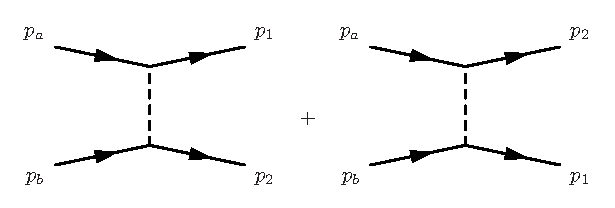
\includegraphics{\feynmfdirectory/01NNtoNNeq/NNtoNN.eps}
\nonumber\\
\label{eqn:scYSmtrxFeynmDiagNN}
\end{eqnarray}
%----------------------------------------
The final expression is written in terms of two Feynman diagrams
which correspond respectively to the two terms in Eq. (\ref{eqn:scYSelem}).
These diagrams are abbreviated a bit for a technical reason of the drawing.
A fully drawn diagram may look like the following figure.
\begin{figure}[h]
\vspace*{35mm}
%        positive in these values mean,  voffset: upward   hoffset: rightward
\special{psfile="\feynmfdirectory/02NNtoNNbig/NNtoNNtrim.eps" hscale=70 vscale=70 voffset=-0 hoffset=100}
\caption{Fully drawn Feynman diagram for the first term in Eq. (\ref{eqn:scYSmtrxFeynmDiagNN})}
\label{fig:scalarYNN2NNFeynm}
\end{figure}
Arrows on external lines indicate flows of conserved quantum numbers associated with
particles like baryon number, flavor and so on. In the present case, it is the electric charge
which is conserved in the Lagrangian density (\ref{eqn:sclYkwLagDens}) as is stated above
Eq. (\ref{eqn:scYelchrg}).
In many situations, we draw a diagram like Fig. \ref{fig:scalarYNN2NNFeynm} without
momentum arrows to represent the two diagrams in Eq. (\ref{eqn:scYSmtrxFeynmDiagNN}).


The correspondence between diagrams and equations are ensured by obeying
the so called Feynman rule described as follows:

\begin{enumerate}
\item For each external lines, associate a factor $1/\sqrt{(2\pi)^3}$.

\item To each vertex, associate a factor
\begin{eqnarray}
(-ig) (2\pi)^4 \delta^4(\sum_{in} p_{in})\,,
\end{eqnarray}
where $p_{in}$ denotes a momentum flowing into the vertex and the sum is taken
over all momenta connected to the vertex. Momenta flowing out from the vertex get
a minus sign. For the upper vertex in Fig. (\ref{fig:scalarYNN2NNFeynm}), for instance,
we read $\sum_{in} p_{in} = p_a - k - p_1$.

\item For each internal broken line, corresponding to a $\phi$ particle with momentum $k$,
write a factor of
\begin{eqnarray}
\int \frac{d^4 k}{(2\pi)^4} \frac{i}{k^2 - m^2 + i\epsilon}
\end{eqnarray}
When the internal line is solid, corresponding to a $\psi$ particle, write the same factor
with $m$ replaced by the nucleon mass $M$.
\end{enumerate}

The scattering amplitude $T_{fi} = \bra f \braend T \ketend i \ket$ 
in Eq. (\ref{eqn:Smatrix_and_T}) is now
written as
\begin{eqnarray}
T_{fi}^{(2)}
&=&
\frac{(-i g)^2}{(2\pi)^6} 
\left\{
\frac{1}{(p_1 - p_a)^2 - m^2}
+
\frac{1}{(p_2 - p_a)^2 - m^2}
\right\}
\nonumber\\
&=&
\frac{(-i g)^2}{(2\pi)^6} 
\left(
\frac{1}{t - m^2}
+
\frac{1}{u - m^2}
\right)
\end{eqnarray}
Finally, from Eq. (\ref{eqn:2to2cs}), we write the scattering cross section 
in scalar Yukawa theory to the lowest (second) order as
\begin{eqnarray}
\frac{d \sigma^{(2)}}{dt}
&=&
\frac{g^4}{16\pi \lambda(s, m_N^2,m_N^2)}
\left(
\frac{1}{t - m^2} + \frac{1}{u - m^2}
\right)^2
\label{eqn:scYNN2NNcs}
\end{eqnarray}

\bigskip

\noindent
\stepcounter{exercise}
Exercise\theexercise:
Examine the kinematical regions for $t$ and $u$ in this scattering.

\bigskip

An enhancement of the cross section at small $|t|$ follows from the mass pole
of the exchanged pion. We also understand an enhancement at small $|u|$ is
a consequence of  the domination of $t$-channel exchanges 
and the indistinguishability of the two nucleons in the final state.


%----------------------------------------
\begin{comment}
Integral expression of the scattering matrix element in Eq. (\ref{eqn:scYSelem}) 
is written in terms of the Feynman diagram as
\begin{figure}[h]
\vspace*{30mm}
%        positive in these values mean,  voffset: upward   hoffset: rightward
\special{psfile="\feynmfdirectory/01NNtoNNeq/NNtoNN.eps" hscale=70 vscale=70 voffset=30 hoffset=70}
%\caption{Feynman diagram}
\label{fig:scalarYNN2NNinEq}
\end{figure}


&&
\unitlength=1mm  %<<<---------------------------------------------- scale
\parbox{40mm}
{
\begin{fmffile}{NNbyPi1}
	\begin{fmfgraph*}(40,20)
			\fmfleft{i1,i2}
			\fmfright{o1,o2} 
			%\fmfv{label=$p_b$, label.angle=90}{i1}
			\fmflabel{$p_b$}{i1}
			\fmflabel{$p_a$}{i2}
			%\fmfv{label=$p_a$, label.angle=270}{i2}
			\fmflabel{$p_2$}{o1}
			\fmflabel{$p_1$}{o2}
			\fmf{fermion,tension=2}{i1,v1,o1}
			\fmf{fermion,tension=2}{i2,v2,o2}
			\fmf{dashes}{v1,v2}
			%\fmflabel{$-ig(2\pi)^4 \delta^4(\sum_{in} p_{in})$}{v1}
			%\fmflabel{$-ig(2\pi)^4 \delta^4(\sum_{in} p_{in})$}{v2}
	\end{fmfgraph*}
\end{fmffile}
}
\hspace{3mm}
+
\hspace{3mm}
\parbox{40mm}
{
\begin{fmffile}{NNbyPi2}
	\begin{fmfgraph*}(40,20)
			\fmfleft{i1,i2}
			\fmfright{o1,o2} 
			\fmflabel{$p_b$}{i1}
			\fmflabel{$p_a$}{i2}
			\fmflabel{$p_1$}{o1}
			\fmflabel{$p_2$}{o2}
			\fmf{fermion,tension=2}{i1,v1,o1}
			\fmf{fermion,tension=2}{i2,v2,o2}
			\fmf{dashes}{v1,v2}
	\end{fmfgraph*}
\end{fmffile}
}
\end{comment}
%----------------------------------------

\bigskip

\bigskip
%=================================================================
\noindent
\underline{$N\overline{N} \to N\overline{N}$ amplitude}

\bigskip

Initial and final states:
\begin{eqnarray}
\begin{array}{l}
\ketend i \ket
=
b^\dagger(\bld{p}_a) c^\dagger(\bld{p}_b) \ketend 0 \ket
\rightdef
%\ketend N(\bld{p}_a) \overline{N}(\bld{b}_b )\ket
\ketend N_a \overline{N}_b \ket
\\
\ketend f \ket
=
b^\dagger(\bld{p}_1) c^\dagger(\bld{p}_2) \ketend 0 \ket
\rightdef
%\ketend N(\bld{p}_1) \overline{N}(\bld{p}_2) \ket
\ketend N_1 \overline{N}_2 \ket
\end{array}
\label{eqn:scYNNbarNNbarinit}
\end{eqnarray}
Since there are four (anti) nucleons in the initial and final states, we need at least 
four $\psi$ (and $\psi^\dagger$) fields from interaction Hamiltonians and all $\phi$ fields should
be contracted out. Thus, S-matrix elements to the lowest order is written 
in the same form as Eq. (\ref{eqn:scYS2ndord}) with $N_b$ and $N_2$ replaced by
$\overline{N}_b$ and $\overline{N}_2$ respectively.
Evaluating the sandwich factor as before,
we get
\begin{eqnarray}
\bra f \braend S^{(2)} \ketend i \ket
%&\stackrel{(2)}{=}&
&=&
%\nonumber\\
%&&
\parbox{80mm}{
\includegraphics{\feynmfdirectory/03NNbar2NNbar/Smtrx2trim.eps}
}
\nonumber\\
\label{eqn:scYSmtrxFeynmDiagNNbar}
\end{eqnarray}
It reads
\begin{eqnarray}
T_{fi}^{(2)}
&=&
\frac{(-i g)^2}{(2\pi)^6} 
\left\{
\frac{1}{(p_a - p_1)^2 - m^2 \cancel{+ i\epsilon}}
+
\frac{1}{(p_a + p_b)^2 - m^2 + i\epsilon}
\right\}
\nonumber\\
&=&
\frac{(-i g)^2}{(2\pi)^6} 
\left(
\frac{1}{t - m^2}
+
\frac{1}{s - m^2 + i\epsilon}
\right)
\label{eqn:scYNNbar}
\end{eqnarray}
Cross section is obtained by adopting Eq. (\ref{eqn:2to2cs}) as before.
We omit $i \epsilon$ in the first term in Eq. (\ref{eqn:scYNNbar}) since
$t < 0$. In the second term, however, $s = m^2$ may occur when
$m > 2M$. This is why we remained $i \epsilon$ in the second term.
However, in this case, correction of the pion propagator due to higher
order terms with nucleon loops will bring a finite imaginary part into the
denominator of the propagator. Nevertheless, for the lowest order
tree diagram, we keep the $i \epsilon$ term. 

\bigskip

\verb/-----------.-----------.-----------.-----------.-----------/\\
\vspace{-3mm}
{\small
\begin{center}
Addendum: Derivation of Eq. (\ref{eqn:scYSmtrxFeynmDiagNNbar})
\end{center}

It is yet instructive to show the derivation of Eq. (\ref{eqn:scYSmtrxFeynmDiagNNbar}).
The way of evaluation here will be a little bit more skillful than one shown before.
To evaluate Eq. (\ref{eqn:scYS2ndord}) with the initial and final states replaced 
by the current case, we write
\begin{eqnarray}
\psi(x) = b(x) + c^\dagger(x)\,,
\hspace{3mm}
\psi^\dagger(x) = b^\dagger(x) + c(x)\,,
\end{eqnarray}
referring the form in Eq. (\ref{eqn:scYfields}).
In the following, we abbreviate arguments of fields and their parts by suffices.
For instance, $\psi(x_i)$ is abbreviated by $\psi_i$ and $b(x_i)$ by $b_i$.
We will use the same abbreviation $b_i$ either for $b(x_i)$ or for $b(\bld{p}_i)$ 
when there is little possibility of confusion.
An abbreviation $c_i$ is used in a similar manner.

Considering the initial and final states in Eq. (\ref{eqn:scYNNbarNNbarinit}),
we need to remain terms $\sim b^\dagger c^\dagger bc$ in the sandwich of 
the normal order product in Eq. (\ref{eqn:scYS2ndord}). Since there are two
$\psi^\dagger$'s and two $\psi$'s, we have four ways to pick up necessary factors:
\begin{eqnarray}
&&
\bra \overline{N}_2 N_1 \braend 
\normalprod{\psi_{1'}^\dagger \psi_{1'} \psi_{2'}^\dagger \psi_{2'}}
\ketend N_a \overline{N}_b \ket
\nonumber\\
&&=
\bra 0 \braend c_2 b_1
\normalprod{
(b_{1'}^\dagger + c_{1'} ) ( b_{1'} + c_{1'}^\dagger) 
(b_{2'}^\dagger + c_{2'}) (b_{2'} + c_{2'}^\dagger)
}
b_a^\dagger c_b^\dagger 
\ketend 0 \ket
\nonumber\\
&& \mbox{(pick up relevant terms)}
\nonumber\\
&&=
\bra 0 \braend c_2 b_1
\normalprod{
\left(
b_{1'}^\dagger
b_{1'}
c_{2'} 
c_{2'}^\dagger
+
c_{1'}  
c_{1'}^\dagger
b_{2'}^\dagger
b_{2'}
+
b_{1'}^\dagger
c_{1'}^\dagger
c_{2'} 
b_{2'}
+
c_{1'}  
b_{1'}
b_{2'}^\dagger
c_{2'}^\dagger
\right)
}
b_a^\dagger c_b^\dagger 
\ketend 0 \ket
\nonumber\\
&& \mbox{(take normal ordering)}
\nonumber\\
&&=
\bra 0 \braend c_2 b_1
\left\{
b_{1'}^\dagger
c_{2'}^\dagger
b_{1'}
c_{2'} 
+
c_{1'}^\dagger
b_{2'}^\dagger
c_{1'}  
b_{2'}
+
b_{1'}^\dagger
c_{1'}^\dagger
c_{2'} 
b_{2'}
+
b_{2'}^\dagger
c_{2'}^\dagger
c_{1'}  
b_{1'}
\right\}
b_a^\dagger c_b^\dagger 
\ketend 0 \ket
\nonumber\\
&& \mbox{($b$'s and $c$'s are commuting to each orher)}
\nonumber\\
&&=
\bra 0 \braend c_2 b_1
\left\{
b_{1'}^\dagger
c_{2'}^\dagger
c_{2'} 
b_{1'}
+
b_{2'}^\dagger
c_{1'}^\dagger
c_{1'}  
b_{2'}
+
b_{1'}^\dagger
c_{1'}^\dagger
c_{2'} 
b_{2'}
+
b_{2'}^\dagger
c_{2'}^\dagger
c_{1'}  
b_{1'}
\right\}
b_a^\dagger c_b^\dagger 
\ketend 0 \ket
\nonumber\\
\label{eqn:NNbarSandwFirst}
\end{eqnarray}
Using suffices $1'$ and $2'$, 
we are writing integration variables in  Eq. (\ref{eqn:scYS2ndord})
as $x_{1'}$ and $x_{2'}$ and they can be exchanged 
since $\Delta_F$ is an even function. Thus,
\begin{eqnarray}
&&
\int d^4 x_{1'} d^4 x_{2'} \Delta_F(1' - 2')
\bra \overline{N}_2 N_1 \braend 
\normalprod{\psi_{1'}^\dagger \psi_{1'} \psi_{2'}^\dagger \psi_{2'}}
\ketend N_a \overline{N}_b \ket
\nonumber\\
&&=
2 \int d^4 x_{1'} d^4 x_{2'} \Delta_F(1' - 2')
\bra 0 \braend c_2 b_1
\left\{
b_{1'}^\dagger
c_{2'}^\dagger
c_{2'} 
b_{1'}
+
b_{1'}^\dagger
c_{1'}^\dagger
c_{2'} 
b_{2'}
\right\}
b_a^\dagger c_b^\dagger 
\ketend 0 \ket
\nonumber\\
&&
\hspace{56mm}
p_1'
\,
%\hspace{5mm}
p_2'
\,
%\hspace{5mm}
p_a'
\,
%\hspace{5mm}
p_b'
\hspace{5mm}
p_1'
\,
%\hspace{5mm}
p_2'
\,
%\hspace{5mm}
p_a'
\,
%\hspace{5mm}
p_b'
\,
%\hspace{5mm}
\label{eqn:NNbarSandwich}
\end{eqnarray}
In the last line of the above equation, assignments for momentum variables
to correspond to external lines are shown for convenience. 
For instance, $p_1'$  indicated below $b_{1'}^\dagger$ reads
\begin{eqnarray}
b_{1'}^\dagger = b^\dagger(x_{1}')
=
\int \frac{d^3 \bld{p}_{1}'}{\sqrt{(2\pi)^3} 2 {p_{1}}^{'0}}
b^\dagger(\bld{p}_{1}') 
e^{i p_{1}' x_{1}'}
\end{eqnarray}
In our abbreviated notations, it then reads that, for instance,
\begin{eqnarray}
[b_1, b_{1'}^\dagger]
=
\frac{1}{\sqrt{(2\pi)^3}} e^{i p_1 x_1'}\,,
\hspace{5mm}
[b_{1'}, b^\dagger_{a}]
=
\frac{1}{\sqrt{(2\pi)^3}} e^{-i p_a x_1'}
\end{eqnarray}
Inside integrations over $x_1'$ and $x_2'$ with a even function $\Delta_F$ 
in  Eq. (\ref{eqn:NNbarSandwich}),
one can thus proceed Eq. (\ref{eqn:NNbarSandwFirst}) 
%through Eq. (\ref{eqn:NNbarSandwich}) 
as
\begin{eqnarray}
&&
\bra \overline{N}_2 N_1 \braend 
\normalprod{\psi_{1'}^\dagger \psi_{1'} \psi_{2'}^\dagger \psi_{2'}}
\ketend N_a \overline{N}_b \ket
\nonumber\\
&&=
2 \bra 0 \braend c_2 
\left( [b_1, b_{1'}^\dagger] + b_{1'}^\dagger b_1 \right)
\left\{
c_{2'}^\dagger
c_{2'} 
\left( [b_{1'}, b_{a}^\dagger] + b_{a}^\dagger b_{1'} \right)
+
c_{1'}^\dagger
c_{2'} 
\left( [b_{2'}, b_{a}^\dagger] + b_{a}^\dagger b_{2'} \right)
\right\}
c_b^\dagger 
\ketend 0 \ket
\nonumber\\
&&=
2 \bra 0 \braend 
[b_1, b_{1'}^\dagger] 
[c_2, c_{2'}^\dagger] 
[b_{1'}, b_{a}^\dagger]
[c_{2'}, c_b^\dagger]
+
[b_1, b_{1'}^\dagger] 
[c_2, c_{1'}^\dagger] 
[b_{2'}, b_{a}^\dagger]
[c_{2'}, c_b^\dagger]
\ketend 0 \ket
\nonumber\\
&&=
\frac{2}{(2\pi)^6}
\left\{
e^{i(p_1 x_1' + p_2 x_2' - p_a x_1' - p_b x_2')}
+
e^{i(p_1 x_1' + p_2 x_1' - p_a x_2' - p_b x_2')}
\right\}
\nonumber\\
\end{eqnarray}
We are now ready to proceed from Eq. (\ref{eqn:scYS2ndord}).
Adopting the expression (\ref{eqn:scFeynmanProp}) of $\Delta_F$, we have
\begin{eqnarray}
\bra f \braend S^{(2)} \ketend i \ket
%&\stackrel{(2)}{=}&
&=&
\frac{(-ig)^2}{2} 
\int \frac{d^4 k}{(2\pi)^4} \frac{i}{k^2 - m^2 + i\epsilon}
\int d^4 x_1' d^4 x_2'
\;e^{-ik(x_1' - x_2')}
\nonumber\\
&&
\hspace{10mm}
\bra \overline{N}_2 N_1 \braend 
\normalprod{\psi_{1'}^\dagger \psi_{1'} \psi_{2'}^\dagger \psi_{2'}}
\ketend N_a \overline{N}_b \ket
\nonumber\\
&=&
\frac{(-ig)^2}{(2\pi)^6} 
\int d^4 k \frac{i (2\pi)^4}{k^2 - m^2 + i\epsilon}
\left\{ 
\delta^4(p_1- p_a - k) \delta^4(p_2 - p_b +k)
\right.
\nonumber\\
&&
\hspace{35mm}
+
\left.
\delta^4(p_1+p_2 - k) \delta^4(p_a + p_b - k)
\right\}
\nonumber\\
&=&
 i (2\pi)^4 \delta^4(P_f - P_i) 
\frac{(-ig)^2}{(2\pi)^6}
%\nonumber\\
%&&
\int
\frac{d^4 k}{k^2 - m^2 + i\epsilon}
\nonumber\\
&&
\hspace{15mm}
\left\{
\delta^4 (p_1 - p_a - k)
+
\delta^4 (p_a + p_b - k)
\right\}
\end{eqnarray}
Eq. (\ref{eqn:scYSmtrxFeynmDiagNNbar}) is thus recovered.
}\\
\begin{center}
\verb/-----------.-----------.-----------.-----------.-----------/\\
\end{center}

\bigskip
%=================================================================
\noindent
\underline{$N\overline{N} \to \pi \pi$ amplitude}

\bigskip

Initial and final states:
\begin{eqnarray}
\begin{array}{l}
\ketend i \ket
=
b^\dagger(\bld{p}_{N}) c^\dagger(\bld{p}_{\bar{N}}) \ketend 0 \ket
\rightdef
%\ketend N(\bld{p}_{N}) \overline{N}(\bld{p}_{\bar{N}} )\ket
\ketend N \overline{N}\ket
\\
\ketend f \ket
=
a^\dagger(\bld{k}_1) a^\dagger(\bld{k}_2) \ketend 0 \ket
\rightdef
%\ketend \pi(\bld{k}_1) \pi (\bld{k}_2) \ket
\ketend \pi_1 \pi_2 \ket
\end{array}
\label{eqn:scYNNbarPiPiinit}
\end{eqnarray}
Field decompositions:
\begin{eqnarray}
\psi = b + c^\dagger\,,
\hspace{3mm}
\phi = a + a^\dagger
\end{eqnarray}
We are to be employing the same abbreviation rules as before.
This time we should go back to the first equation in Eq. (\ref{eqn:scYS2ndord})
for picking up
one $b$ from a $\psi$, one $c$ from a $\psi^\dagger$ and two $a^\dagger$'s from 
two $\phi$'s in the T-product. The remaining pair of $\psi$ and $\psi^\dagger$ are
contracted to give a propagator. 
With a help of Wick's theorem in the form (\ref{eqn:WickTwoNormals}),
we write
\begin{eqnarray}
&&
\bra \pi_2 \pi_1  \braend
T[
\normalprod{
\psi^\dagger_{1'} \psi_{1'} \phi_{1'}
}
\normalprod{
\psi^\dagger_{2'} \psi_{2'} \phi_{2'}
}
]
\ketend N \overline{N} \ket
\nonumber\\
&&
= 
\bra \pi_2 \pi_1  \braend
\normalprod{
\acontraction[1ex]{\psi^\dagger_{1'} }{\psi}{_{1'} \phi_{1'}}{\psi}
\psi^\dagger_{1'} \psi_{1'} \phi_{1'}\psi^\dagger_{2'} \psi_{2'} \phi_{2'}
} %end of normalprod
+
\normalprod{
\acontraction[1ex]{}{\psi}{^\dagger_{1'} \psi_{1'} \phi_{1'}\psi^\dagger_{2'}}{\psi}
\psi^\dagger_{1'} \psi_{1'} \phi_{1'}\psi^\dagger_{2'} \psi_{2'} \phi_{2'}
} %end of normalprod
\ketend N \overline{N} \ket
\nonumber\\
&&
= 
\left\{
\bra \pi_2 \pi_1  \braend
\normalprod{
\phi_{1'} \phi_{2'}
}
\right\}
\left\{
\acontraction[1ex]{}{\psi}{_{1'}}{\psi}
\psi_{1'} \psi^\dagger_{2'}
\normalprod{
\psi^\dagger_{1'}   \psi_{2'} 
}
+
\acontraction[1ex]{}{\psi}{^\dagger_{1'}}{\psi}
\psi^\dagger_{1'}   \psi_{2'} 
\normalprod{
\psi_{1'} \psi^\dagger_{2'}
} %end of normalprod
\right\}
\ketend N \overline{N} \ket
\nonumber\\
\end{eqnarray}
Propagator of the complex scalar fields is given in Eq. (\ref{eqn:CplxScProp}) and
\begin{eqnarray}
&&
=
\Delta_F(1' - 2')
\bra 0 \braend
\left\{
 a_2 a_1 a_{1'}^\dagger a_{2'}^\dagger
\right\}
\left\{
c_{1'}b_{2'} + b_{1'}c_{2'} 
\right\}
b_{N}^\dagger c_{\bar{N}}^\dagger 
\ketend 0 \ket
\nonumber\\
&&
=
\Delta_F(1' - 2')
\bra 0 \braend
\left\{
[a_1, a_{1'}^\dagger] [a_2, a_{2'}^\dagger]
+
[a_2, a_{1'}^\dagger] [a_1, a_{2'}^\dagger]
\right\}
\left\{
[b_{2'}, b_{N}^\dagger]  [c_{1'},  c_{\bar{N}}^\dagger ]
+ [b_{1'}, b_{N}^\dagger]
[c_{2'} ,  c_{\bar{N}}^\dagger ]
\right\}
\ketend 0 \ket
\nonumber\\
&&
=
\frac{1}{(2\pi)^6} \Delta_F(1' - 2')
\left\{
e^{i(k_1 x_1' + k_2 x_2')}
+
e^{i(k_2 x_1' + k_1 x_2')}
\right\}
\left\{
e^{-i(p_N x_2' + p_{\bar{N}} x_1')}
+
e^{-i(p_N x_1' + p_{\bar{N}} x_2')}
\right\}
\nonumber\\
\end{eqnarray}
Inside integration over $x_1'$ and $x_2'$, 
Adopting Eq. (\ref{eqn:scFeynmanProp}) with $m$ replaced by the nucleon mass $M$, we may write
\begin{eqnarray}
\bra \pi_2 \pi_1  \braend
S^{(2)}
\ketend N \overline{N} \ket
&=&
\frac{(-ig)^2}{2 (2\pi)^6}
\int \frac{d^4 p'}{(2\pi)^4} \frac{i}{p^{'2} - M^2 + i\epsilon}
\int d^4 x_1' d^4 x_2'\; e^{-ip' (x_1' - x_2')}
\nonumber\\
&&
\times 2
\left\{
e^{i(k_1 x_1' + k_2 x_2' -p_N x_1' - p_{\bar{N}} x_2')}
+
e^{i(k_1 x_1' + k_2 x_2' -p_N x_2' - p_{\bar{N}} x_1')}
\right\}
\nonumber\\
&=&
\frac{(-ig)^2}{(2\pi)^6}
\int d^4 p'  \frac{i (2\pi)^4}{p^{'2} - M^2 + i\epsilon}
\left\{
\delta^4 (k_1  -p_N - p' ) \delta^4( k_2 - p_{\bar{N}} + p')
\right.
\nonumber\\
&&
\hspace{40mm}
+
\left.
\delta^4( k_1 - p_{\bar{N}} - p') \delta^4 (k_2  -p_N + p' ) 
\right\}
\nonumber\\
&=&
\parbox{80mm}{
\includegraphics{\feynmfdirectory/04NNbar2PiPi/Smtrx2trim.eps}
}
\nonumber\\
&=&
i (2\pi)^4 \delta^4(P_f - P_i)
\frac{(-ig)^2}{(2\pi)^6}
\left\{
\frac{1}{t - M^2 + i\epsilon}
+
\frac{1}{u - M^2 + i\epsilon}
\right\}
\label{eqn:scYAmpNNbarPiPi}
\end{eqnarray}
For a technical reason, we wrote $p_{Nbar}$ in places of $p_{\bar{N}}$ in 
Feynman diagrams in Eq. (\ref{eqn:scYAmpNNbarPiPi}).
One may omit $i\epsilon$ in denominators of propagators in Eq.  (\ref{eqn:scYAmpNNbarPiPi}).
The same comments in the last paragraph just after Eq. (\ref{eqn:scYNN2NNcs}) is 
also relevant here by exchanging terms pion and nucleon there.


\subsubsection{Scattering of Scalar Nucleons}
Let's go back to the scalar Yukawa theory of the section \ref{sec:ScYukawa} and 
consider nucleon scattering process $\psi \psi \to \psi \psi$.
\begin{eqnarray}
\begin{array}{l}
\ketend i \ket
=
b^\dagger(\bld{p}_a) b^\dagger(\bld{p}_b) \ketend 0 \ket
\rightdef
\ketend N_a N_b \ket
\\
\ketend f \ket
=
b^\dagger(\bld{p}_1) b^\dagger(\bld{p}_2) \ketend 0 \ket
\rightdef
\ketend N_1 N_2 \ket
\end{array}
\end{eqnarray}
The first contribution to $S - 1$ in Eq. (\ref{eqn:SmatrixPertSerCov}) arise from 
the term of the second order in ${\cal H}_{int}$. It reads
\begin{eqnarray}
\bra f \braend S^{(2)} \ketend i \ket
&=&
\frac{(-i g)^2}{2} \int d^4 x_1 d^4 x_2
\bra f \braend
T[
\normalprod{\psi^\dagger(x_1) \psi(x_1) \phi(x_1)}
\nonumber\\
&&
\hspace{35mm}
\times
\normalprod{\psi^\dagger(x_2) \psi(x_2) \phi(x_2)}
]
\ketend i \ket
\nonumber\\
&=&
\frac{(-i g)^2}{2} \int d^4 x_1 d^4 x_2
\Delta_F(x_1 - x_2)
\nonumber\\
&&
\hspace{12mm}
\bra N_2 N_1 \braend
\normalprod{
\psi^\dagger(x_1) \psi(x_1) 
\psi^\dagger(x_2) \psi(x_2)
}
\ketend N_a N_b \ket\,,
\nonumber\\
\label{eqn:scYS2ndord}
\end{eqnarray}
%-------------------------------------------
The sandwich $\bra N_1 N_2 \braend \dots \ketend N_b N_a \ket$ reads
\begin{eqnarray}
&&\bra N_1 N_2 \braend
\normalprod{
\psi^\dagger(x_1) \psi(x_1) 
\psi^\dagger(x_2) \psi(x_2)
}
\ketend N_b N_a \ket
\nonumber\\
&=&
\int \frac{d^3 \bld{p}_1' d^3 \bld{p}_2'}{(2\pi)^3 4 {p_1^0}' {p_2^0}'} 
 \frac{d^3 \bld{p}_a' d^3 \bld{p}_b'}{(2\pi)^3 4 {p_a^0}' {p_b^0}'} 
 e^{i(p_1' x_1 + p_2' x_2 - p_a' x_1 - p_b' x_2)}
\nonumber\\
&&
 \bra 0 \braend 
 b(\bld{p}_2)  b(\bld{p}_1) \left\{
 b^\dagger(\bld{p}_1') b^\dagger(\bld{p}_2')
b(\bld{p}_a') b(\bld{p}_b')
\right\}
 b^\dagger(\bld{p}_a) b^\dagger(\bld{p}_b)
 \ketend 0 \ket
\nonumber\\
&=&
\int \frac{d^3 \bld{p}_1' d^3 \bld{p}_2'}{(2\pi)^3 4 {p_1^0}' {p_2^0}'} 
 \frac{d^3 \bld{p}_a' d^3 \bld{p}_b'}{(2\pi)^3 4 {p_a^0}' {p_b^0}'} 
 e^{i(p_1' x_1 + p_2' x_2 - p_a' x_1 - p_b' x_2)}
\nonumber\\
&&
\bra 0 \braend 
 b(\bld{p}_2)  \left\{
 2{p_1^0}' \delta^3(\bld{p}_1' - \bld{p}_1) 
 + b^\dagger({\bld{p}_1'}) b({\bld{p}_1})
 \right\}
 b^\dagger({\bld{p}_2'})
 \nonumber\\
 &&
  b(\bld{p}_a')   \left\{
 2{p_b^0}' \delta^3(\bld{p}_b' - \bld{p}_a) 
 + b^\dagger({\bld{p}_a}) b({\bld{p}_b'})
  \right\}
  b^\dagger({\bld{p}_b})
   \ketend 0 \ket
\nonumber\\
&=&
\int \frac{d^3 \bld{p}_1' d^3 \bld{p}_2'}{(2\pi)^3 4 {p_1^0}' {p_2^0}'} 
 \frac{d^3 \bld{p}_a' d^3 \bld{p}_b'}{(2\pi)^3 4 {p_a^0}' {p_b^0}'} 
 e^{i(p_1' x_1 + p_2' x_2 - p_a' x_1 - p_b' x_2)}
\nonumber\\
&&
\bra 0 \braend 
\left\{
4{p_1^0}' {p_2^0}' \delta^3(\bld{p}_1' - \bld{p}_1) \delta^3(\bld{p}_2' - \bld{p}_2) 
+
4{p_1^0}' {p_2^0}' \delta^3(\bld{p}_1' - \bld{p}_2) \delta^3(\bld{p}_2' - \bld{p}_1) 
\right\}
\nonumber\\
&&
\left\{
4{p_a^0}' {p_b^0}' \delta^3(\bld{p}_a' - \bld{p}_b) \delta^3(\bld{p}_b' - \bld{p}_a) 
+
4{p_a^0}' {p_b^0}' \delta^3(\bld{p}_a' - \bld{p}_a) \delta^3(\bld{p}_b' - \bld{p}_b) 
\right\}
\ketend 0 \ket
\nonumber\\
&=&
\frac{1}{(2\pi)^6}
\left\{
e^{i(p_1 x_1 + p_2 x_2)} + e^{i(p_2 x_1 + p_1 x_2)}
\right\}
\left\{
e^{-i(p_a x_1 + p_b x_2)} + e^{-i(p_b x_1 + p_a x_2)}
\right\}
\nonumber
\end{eqnarray}
Substituting this result in Eq. (\ref{eqn:scYS2ndord}) and 
adopting the expression (\ref{eqn:scFeynmanProp}),
we obtain
\begin{eqnarray}
\bra f \braend S^{(2)} \ketend i \ket
&=&
\frac{(-i g)^2}{2 (2\pi)^6} \int \frac{d^4 k}{(2\pi)^4} 
\frac{i}{k^2 - m^2 + i\epsilon}
\int d^4 x_1 d^4 x_2
\left\{
e^{i(p_1 + k - p_a)x_1}e^{i(p_2 - k - p_b)}
\right.
\nonumber\\
&&
+
e^{i(p_2 + k - p_a)x_1}e^{i(p_1 - k - p_b)}
+
e^{i(p_1 + k - p_b)x_1}e^{i(p_2 - k - p_1)}
\nonumber\\
&&
\left.
+
e^{i(p_2 + k - p_b)x_1}e^{i(p_1 - k - p_a)}
\right\}
\nonumber\\
&=&
\frac{i(-i g)^2}{(2\pi)^6} \int 
\frac{(2\pi)^4 d^4 k}{k^2 - m^2 + i\epsilon}
\left\{
\delta^4(p_1 + k - p_a)\delta^4(p_2 - k - p_b)
\right.
\nonumber\\
&&
\left.
\hspace{35mm}
+
\delta^4(p_2 + k - p_a)\delta^4(p_1 - k - p_b)
\right\}
\label{eqn:scYSelem}
\\
&=&
\frac{i(-i g)^2}{(2\pi)^6} 
\left\{
\frac{1}{(p_1 - p_a)^2 - m^2}
+
\frac{1}{(p_2 - p_a)^2 - m^2}
\right\}
\nonumber\\
&&
\times (2\pi)^4 \delta^4(p_1 + p_2 - p_a - p_b)
\nonumber\\
&=&
\nonumber\\
&&
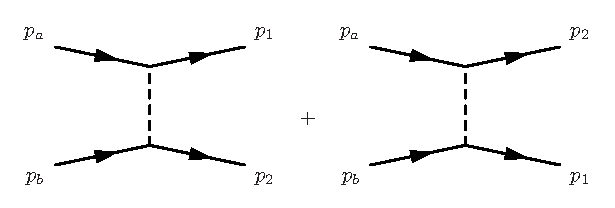
\includegraphics{\feynmfdirectory/01NNtoNNeq/NNtoNN.eps}
\nonumber\\
\label{eqn:scYSmtrxFeynmDiagNN}
\end{eqnarray}
%----------------------------------------
The final expression is written in terms of two Feynman diagrams
which correspond respectively to the two terms in Eq. (\ref{eqn:scYSelem}).
These diagrams are abbreviated a bit for a technical reason of the drawing.
A fully drawn diagram may look like the following figure.
\begin{figure}[h]
\vspace*{35mm}
%        positive in these values mean,  voffset: upward   hoffset: rightward
\special{psfile="\feynmfdirectory/02NNtoNNbig/NNtoNNtrim.eps" hscale=70 vscale=70 voffset=-0 hoffset=100}
\caption{Fully drawn Feynman diagram for the first term in Eq. (\ref{eqn:scYSmtrxFeynmDiagNN})}
\label{fig:scalarYNN2NNFeynm}
\end{figure}
Arrows on external lines indicate flows of conserved quantum numbers associated with
particles like baryon number, flavor and so on. In the present case, it is the electric charge
which is conserved in the Lagrangian density (\ref{eqn:sclYkwLagDens}) as is stated above
Eq. (\ref{eqn:scYelchrg}).
In many situations, we draw a diagram like Fig. \ref{fig:scalarYNN2NNFeynm} without
momentum arrows to represent the two diagrams in Eq. (\ref{eqn:scYSmtrxFeynmDiagNN}).


The correspondence between diagrams and equations are ensured by obeying
the so called Feynman rule described as follows:

\begin{enumerate}
\item For each external lines, associate a factor $1/\sqrt{(2\pi)^3}$.

\item To each vertex, associate a factor
\begin{eqnarray}
(-ig) (2\pi)^4 \delta^4(\sum_{in} p_{in})\,,
\end{eqnarray}
where $p_{in}$ denotes a momentum flowing into the vertex and the sum is taken
over all momenta connected to the vertex. Momenta flowing out from the vertex get
a minus sign. For the upper vertex in Fig. (\ref{fig:scalarYNN2NNFeynm}), for instance,
we read $\sum_{in} p_{in} = p_a - k - p_1$.

\item For each internal broken line, corresponding to a $\phi$ particle with momentum $k$,
write a factor of
\begin{eqnarray}
\int \frac{d^4 k}{(2\pi)^4} \frac{i}{k^2 - m^2 + i\epsilon}
\end{eqnarray}
When the internal line is solid, corresponding to a $\psi$ particle, write the same factor
with $m$ replaced by the nucleon mass $M$.
\end{enumerate}

The scattering amplitude $T_{fi} = \bra f \braend T \ketend i \ket$ 
in Eq. (\ref{eqn:Smatrix_and_T}) is now
written as
\begin{eqnarray}
T_{fi}^{(2)}
&=&
\frac{(-i g)^2}{(2\pi)^6} 
\left\{
\frac{1}{(p_1 - p_a)^2 - m^2}
+
\frac{1}{(p_2 - p_a)^2 - m^2}
\right\}
\nonumber\\
&=&
\frac{(-i g)^2}{(2\pi)^6} 
\left(
\frac{1}{t - m^2}
+
\frac{1}{u - m^2}
\right)
\end{eqnarray}
Finally, from Eq. (\ref{eqn:2to2cs}), we write the scattering cross section 
in scalar Yukawa theory to the lowest (second) order as
\begin{eqnarray}
\frac{d \sigma^{(2)}}{dt}
&=&
\frac{g^4}{16\pi \lambda(s, m_N^2,m_N^2)}
\left(
\frac{1}{t - m^2} + \frac{1}{u - m^2}
\right)^2
\label{eqn:scYNN2NNcs}
\end{eqnarray}

\bigskip

\noindent
\stepcounter{exercise}
Exercise\theexercise:
Examine the kinematical regions for $t$ and $u$ in this scattering.

\bigskip

An enhancement of the cross section at small $|t|$ follows from the mass pole
of the exchanged pion. We also understand an enhancement at small $|u|$ is
a consequence of  the domination of $t$-channel exchanges 
and the indistinguishability of the two nucleons in the final state.


%----------------------------------------
\begin{comment}
Integral expression of the scattering matrix element in Eq. (\ref{eqn:scYSelem}) 
is written in terms of the Feynman diagram as
\begin{figure}[h]
\vspace*{30mm}
%        positive in these values mean,  voffset: upward   hoffset: rightward
\special{psfile="\feynmfdirectory/01NNtoNNeq/NNtoNN.eps" hscale=70 vscale=70 voffset=30 hoffset=70}
%\caption{Feynman diagram}
\label{fig:scalarYNN2NNinEq}
\end{figure}


&&
\unitlength=1mm  %<<<---------------------------------------------- scale
\parbox{40mm}
{
\begin{fmffile}{NNbyPi1}
	\begin{fmfgraph*}(40,20)
			\fmfleft{i1,i2}
			\fmfright{o1,o2} 
			%\fmfv{label=$p_b$, label.angle=90}{i1}
			\fmflabel{$p_b$}{i1}
			\fmflabel{$p_a$}{i2}
			%\fmfv{label=$p_a$, label.angle=270}{i2}
			\fmflabel{$p_2$}{o1}
			\fmflabel{$p_1$}{o2}
			\fmf{fermion,tension=2}{i1,v1,o1}
			\fmf{fermion,tension=2}{i2,v2,o2}
			\fmf{dashes}{v1,v2}
			%\fmflabel{$-ig(2\pi)^4 \delta^4(\sum_{in} p_{in})$}{v1}
			%\fmflabel{$-ig(2\pi)^4 \delta^4(\sum_{in} p_{in})$}{v2}
	\end{fmfgraph*}
\end{fmffile}
}
\hspace{3mm}
+
\hspace{3mm}
\parbox{40mm}
{
\begin{fmffile}{NNbyPi2}
	\begin{fmfgraph*}(40,20)
			\fmfleft{i1,i2}
			\fmfright{o1,o2} 
			\fmflabel{$p_b$}{i1}
			\fmflabel{$p_a$}{i2}
			\fmflabel{$p_1$}{o1}
			\fmflabel{$p_2$}{o2}
			\fmf{fermion,tension=2}{i1,v1,o1}
			\fmf{fermion,tension=2}{i2,v2,o2}
			\fmf{dashes}{v1,v2}
	\end{fmfgraph*}
\end{fmffile}
}
\end{comment}
%----------------------------------------

\bigskip

\bigskip
%=================================================================
\noindent
\underline{$N\overline{N} \to N\overline{N}$ amplitude}

\bigskip

Initial and final states:
\begin{eqnarray}
\begin{array}{l}
\ketend i \ket
=
b^\dagger(\bld{p}_a) c^\dagger(\bld{p}_b) \ketend 0 \ket
\rightdef
%\ketend N(\bld{p}_a) \overline{N}(\bld{b}_b )\ket
\ketend N_a \overline{N}_b \ket
\\
\ketend f \ket
=
b^\dagger(\bld{p}_1) c^\dagger(\bld{p}_2) \ketend 0 \ket
\rightdef
%\ketend N(\bld{p}_1) \overline{N}(\bld{p}_2) \ket
\ketend N_1 \overline{N}_2 \ket
\end{array}
\label{eqn:scYNNbarNNbarinit}
\end{eqnarray}
Since there are four (anti) nucleons in the initial and final states, we need at least 
four $\psi$ (and $\psi^\dagger$) fields from interaction Hamiltonians and all $\phi$ fields should
be contracted out. Thus, S-matrix elements to the lowest order is written 
in the same form as Eq. (\ref{eqn:scYS2ndord}) with $N_b$ and $N_2$ replaced by
$\overline{N}_b$ and $\overline{N}_2$ respectively.
Evaluating the sandwich factor as before,
we get
\begin{eqnarray}
\bra f \braend S^{(2)} \ketend i \ket
%&\stackrel{(2)}{=}&
&=&
%\nonumber\\
%&&
\parbox{80mm}{
\includegraphics{\feynmfdirectory/03NNbar2NNbar/Smtrx2trim.eps}
}
\nonumber\\
\label{eqn:scYSmtrxFeynmDiagNNbar}
\end{eqnarray}
It reads
\begin{eqnarray}
T_{fi}^{(2)}
&=&
\frac{(-i g)^2}{(2\pi)^6} 
\left\{
\frac{1}{(p_a - p_1)^2 - m^2 \cancel{+ i\epsilon}}
+
\frac{1}{(p_a + p_b)^2 - m^2 + i\epsilon}
\right\}
\nonumber\\
&=&
\frac{(-i g)^2}{(2\pi)^6} 
\left(
\frac{1}{t - m^2}
+
\frac{1}{s - m^2 + i\epsilon}
\right)
\label{eqn:scYNNbar}
\end{eqnarray}
Cross section is obtained by adopting Eq. (\ref{eqn:2to2cs}) as before.
We omit $i \epsilon$ in the first term in Eq. (\ref{eqn:scYNNbar}) since
$t < 0$. In the second term, however, $s = m^2$ may occur when
$m > 2M$. This is why we remained $i \epsilon$ in the second term.
However, in this case, correction of the pion propagator due to higher
order terms with nucleon loops will bring a finite imaginary part into the
denominator of the propagator. Nevertheless, for the lowest order
tree diagram, we keep the $i \epsilon$ term. 

\bigskip

\verb/-----------.-----------.-----------.-----------.-----------/\\
\vspace{-3mm}
{\small
\begin{center}
Addendum: Derivation of Eq. (\ref{eqn:scYSmtrxFeynmDiagNNbar})
\end{center}

It is yet instructive to show the derivation of Eq. (\ref{eqn:scYSmtrxFeynmDiagNNbar}).
The way of evaluation here will be a little bit more skillful than one shown before.
To evaluate Eq. (\ref{eqn:scYS2ndord}) with the initial and final states replaced 
by the current case, we write
\begin{eqnarray}
\psi(x) = b(x) + c^\dagger(x)\,,
\hspace{3mm}
\psi^\dagger(x) = b^\dagger(x) + c(x)\,,
\end{eqnarray}
referring the form in Eq. (\ref{eqn:scYfields}).
In the following, we abbreviate arguments of fields and their parts by suffices.
For instance, $\psi(x_i)$ is abbreviated by $\psi_i$ and $b(x_i)$ by $b_i$.
We will use the same abbreviation $b_i$ either for $b(x_i)$ or for $b(\bld{p}_i)$ 
when there is little possibility of confusion.
An abbreviation $c_i$ is used in a similar manner.

Considering the initial and final states in Eq. (\ref{eqn:scYNNbarNNbarinit}),
we need to remain terms $\sim b^\dagger c^\dagger bc$ in the sandwich of 
the normal order product in Eq. (\ref{eqn:scYS2ndord}). Since there are two
$\psi^\dagger$'s and two $\psi$'s, we have four ways to pick up necessary factors:
\begin{eqnarray}
&&
\bra \overline{N}_2 N_1 \braend 
\normalprod{\psi_{1'}^\dagger \psi_{1'} \psi_{2'}^\dagger \psi_{2'}}
\ketend N_a \overline{N}_b \ket
\nonumber\\
&&=
\bra 0 \braend c_2 b_1
\normalprod{
(b_{1'}^\dagger + c_{1'} ) ( b_{1'} + c_{1'}^\dagger) 
(b_{2'}^\dagger + c_{2'}) (b_{2'} + c_{2'}^\dagger)
}
b_a^\dagger c_b^\dagger 
\ketend 0 \ket
\nonumber\\
&& \mbox{(pick up relevant terms)}
\nonumber\\
&&=
\bra 0 \braend c_2 b_1
\normalprod{
\left(
b_{1'}^\dagger
b_{1'}
c_{2'} 
c_{2'}^\dagger
+
c_{1'}  
c_{1'}^\dagger
b_{2'}^\dagger
b_{2'}
+
b_{1'}^\dagger
c_{1'}^\dagger
c_{2'} 
b_{2'}
+
c_{1'}  
b_{1'}
b_{2'}^\dagger
c_{2'}^\dagger
\right)
}
b_a^\dagger c_b^\dagger 
\ketend 0 \ket
\nonumber\\
&& \mbox{(take normal ordering)}
\nonumber\\
&&=
\bra 0 \braend c_2 b_1
\left\{
b_{1'}^\dagger
c_{2'}^\dagger
b_{1'}
c_{2'} 
+
c_{1'}^\dagger
b_{2'}^\dagger
c_{1'}  
b_{2'}
+
b_{1'}^\dagger
c_{1'}^\dagger
c_{2'} 
b_{2'}
+
b_{2'}^\dagger
c_{2'}^\dagger
c_{1'}  
b_{1'}
\right\}
b_a^\dagger c_b^\dagger 
\ketend 0 \ket
\nonumber\\
&& \mbox{($b$'s and $c$'s are commuting to each orher)}
\nonumber\\
&&=
\bra 0 \braend c_2 b_1
\left\{
b_{1'}^\dagger
c_{2'}^\dagger
c_{2'} 
b_{1'}
+
b_{2'}^\dagger
c_{1'}^\dagger
c_{1'}  
b_{2'}
+
b_{1'}^\dagger
c_{1'}^\dagger
c_{2'} 
b_{2'}
+
b_{2'}^\dagger
c_{2'}^\dagger
c_{1'}  
b_{1'}
\right\}
b_a^\dagger c_b^\dagger 
\ketend 0 \ket
\nonumber\\
\label{eqn:NNbarSandwFirst}
\end{eqnarray}
Using suffices $1'$ and $2'$, 
we are writing integration variables in  Eq. (\ref{eqn:scYS2ndord})
as $x_{1'}$ and $x_{2'}$ and they can be exchanged 
since $\Delta_F$ is an even function. Thus,
\begin{eqnarray}
&&
\int d^4 x_{1'} d^4 x_{2'} \Delta_F(1' - 2')
\bra \overline{N}_2 N_1 \braend 
\normalprod{\psi_{1'}^\dagger \psi_{1'} \psi_{2'}^\dagger \psi_{2'}}
\ketend N_a \overline{N}_b \ket
\nonumber\\
&&=
2 \int d^4 x_{1'} d^4 x_{2'} \Delta_F(1' - 2')
\bra 0 \braend c_2 b_1
\left\{
b_{1'}^\dagger
c_{2'}^\dagger
c_{2'} 
b_{1'}
+
b_{1'}^\dagger
c_{1'}^\dagger
c_{2'} 
b_{2'}
\right\}
b_a^\dagger c_b^\dagger 
\ketend 0 \ket
\nonumber\\
&&
\hspace{56mm}
p_1'
\,
%\hspace{5mm}
p_2'
\,
%\hspace{5mm}
p_a'
\,
%\hspace{5mm}
p_b'
\hspace{5mm}
p_1'
\,
%\hspace{5mm}
p_2'
\,
%\hspace{5mm}
p_a'
\,
%\hspace{5mm}
p_b'
\,
%\hspace{5mm}
\label{eqn:NNbarSandwich}
\end{eqnarray}
In the last line of the above equation, assignments for momentum variables
to correspond to external lines are shown for convenience. 
For instance, $p_1'$  indicated below $b_{1'}^\dagger$ reads
\begin{eqnarray}
b_{1'}^\dagger = b^\dagger(x_{1}')
=
\int \frac{d^3 \bld{p}_{1}'}{\sqrt{(2\pi)^3} 2 {p_{1}}^{'0}}
b^\dagger(\bld{p}_{1}') 
e^{i p_{1}' x_{1}'}
\end{eqnarray}
In our abbreviated notations, it then reads that, for instance,
\begin{eqnarray}
[b_1, b_{1'}^\dagger]
=
\frac{1}{\sqrt{(2\pi)^3}} e^{i p_1 x_1'}\,,
\hspace{5mm}
[b_{1'}, b^\dagger_{a}]
=
\frac{1}{\sqrt{(2\pi)^3}} e^{-i p_a x_1'}
\end{eqnarray}
Inside integrations over $x_1'$ and $x_2'$ with a even function $\Delta_F$ 
in  Eq. (\ref{eqn:NNbarSandwich}),
one can thus proceed Eq. (\ref{eqn:NNbarSandwFirst}) 
%through Eq. (\ref{eqn:NNbarSandwich}) 
as
\begin{eqnarray}
&&
\bra \overline{N}_2 N_1 \braend 
\normalprod{\psi_{1'}^\dagger \psi_{1'} \psi_{2'}^\dagger \psi_{2'}}
\ketend N_a \overline{N}_b \ket
\nonumber\\
&&=
2 \bra 0 \braend c_2 
\left( [b_1, b_{1'}^\dagger] + b_{1'}^\dagger b_1 \right)
\left\{
c_{2'}^\dagger
c_{2'} 
\left( [b_{1'}, b_{a}^\dagger] + b_{a}^\dagger b_{1'} \right)
+
c_{1'}^\dagger
c_{2'} 
\left( [b_{2'}, b_{a}^\dagger] + b_{a}^\dagger b_{2'} \right)
\right\}
c_b^\dagger 
\ketend 0 \ket
\nonumber\\
&&=
2 \bra 0 \braend 
[b_1, b_{1'}^\dagger] 
[c_2, c_{2'}^\dagger] 
[b_{1'}, b_{a}^\dagger]
[c_{2'}, c_b^\dagger]
+
[b_1, b_{1'}^\dagger] 
[c_2, c_{1'}^\dagger] 
[b_{2'}, b_{a}^\dagger]
[c_{2'}, c_b^\dagger]
\ketend 0 \ket
\nonumber\\
&&=
\frac{2}{(2\pi)^6}
\left\{
e^{i(p_1 x_1' + p_2 x_2' - p_a x_1' - p_b x_2')}
+
e^{i(p_1 x_1' + p_2 x_1' - p_a x_2' - p_b x_2')}
\right\}
\nonumber\\
\end{eqnarray}
We are now ready to proceed from Eq. (\ref{eqn:scYS2ndord}).
Adopting the expression (\ref{eqn:scFeynmanProp}) of $\Delta_F$, we have
\begin{eqnarray}
\bra f \braend S^{(2)} \ketend i \ket
%&\stackrel{(2)}{=}&
&=&
\frac{(-ig)^2}{2} 
\int \frac{d^4 k}{(2\pi)^4} \frac{i}{k^2 - m^2 + i\epsilon}
\int d^4 x_1' d^4 x_2'
\;e^{-ik(x_1' - x_2')}
\nonumber\\
&&
\hspace{10mm}
\bra \overline{N}_2 N_1 \braend 
\normalprod{\psi_{1'}^\dagger \psi_{1'} \psi_{2'}^\dagger \psi_{2'}}
\ketend N_a \overline{N}_b \ket
\nonumber\\
&=&
\frac{(-ig)^2}{(2\pi)^6} 
\int d^4 k \frac{i (2\pi)^4}{k^2 - m^2 + i\epsilon}
\left\{ 
\delta^4(p_1- p_a - k) \delta^4(p_2 - p_b +k)
\right.
\nonumber\\
&&
\hspace{35mm}
+
\left.
\delta^4(p_1+p_2 - k) \delta^4(p_a + p_b - k)
\right\}
\nonumber\\
&=&
 i (2\pi)^4 \delta^4(P_f - P_i) 
\frac{(-ig)^2}{(2\pi)^6}
%\nonumber\\
%&&
\int
\frac{d^4 k}{k^2 - m^2 + i\epsilon}
\nonumber\\
&&
\hspace{15mm}
\left\{
\delta^4 (p_1 - p_a - k)
+
\delta^4 (p_a + p_b - k)
\right\}
\end{eqnarray}
Eq. (\ref{eqn:scYSmtrxFeynmDiagNNbar}) is thus recovered.
}\\
\begin{center}
\verb/-----------.-----------.-----------.-----------.-----------/\\
\end{center}

\bigskip
%=================================================================
\noindent
\underline{$N\overline{N} \to \pi \pi$ amplitude}

\bigskip

Initial and final states:
\begin{eqnarray}
\begin{array}{l}
\ketend i \ket
=
b^\dagger(\bld{p}_{N}) c^\dagger(\bld{p}_{\bar{N}}) \ketend 0 \ket
\rightdef
%\ketend N(\bld{p}_{N}) \overline{N}(\bld{p}_{\bar{N}} )\ket
\ketend N \overline{N}\ket
\\
\ketend f \ket
=
a^\dagger(\bld{k}_1) a^\dagger(\bld{k}_2) \ketend 0 \ket
\rightdef
%\ketend \pi(\bld{k}_1) \pi (\bld{k}_2) \ket
\ketend \pi_1 \pi_2 \ket
\end{array}
\label{eqn:scYNNbarPiPiinit}
\end{eqnarray}
Field decompositions:
\begin{eqnarray}
\psi = b + c^\dagger\,,
\hspace{3mm}
\phi = a + a^\dagger
\end{eqnarray}
We are to be employing the same abbreviation rules as before.
This time we should go back to the first equation in Eq. (\ref{eqn:scYS2ndord})
for picking up
one $b$ from a $\psi$, one $c$ from a $\psi^\dagger$ and two $a^\dagger$'s from 
two $\phi$'s in the T-product. The remaining pair of $\psi$ and $\psi^\dagger$ are
contracted to give a propagator. 
With a help of Wick's theorem in the form (\ref{eqn:WickTwoNormals}),
we write
\begin{eqnarray}
&&
\bra \pi_2 \pi_1  \braend
T[
\normalprod{
\psi^\dagger_{1'} \psi_{1'} \phi_{1'}
}
\normalprod{
\psi^\dagger_{2'} \psi_{2'} \phi_{2'}
}
]
\ketend N \overline{N} \ket
\nonumber\\
&&
= 
\bra \pi_2 \pi_1  \braend
\normalprod{
\acontraction[1ex]{\psi^\dagger_{1'} }{\psi}{_{1'} \phi_{1'}}{\psi}
\psi^\dagger_{1'} \psi_{1'} \phi_{1'}\psi^\dagger_{2'} \psi_{2'} \phi_{2'}
} %end of normalprod
+
\normalprod{
\acontraction[1ex]{}{\psi}{^\dagger_{1'} \psi_{1'} \phi_{1'}\psi^\dagger_{2'}}{\psi}
\psi^\dagger_{1'} \psi_{1'} \phi_{1'}\psi^\dagger_{2'} \psi_{2'} \phi_{2'}
} %end of normalprod
\ketend N \overline{N} \ket
\nonumber\\
&&
= 
\left\{
\bra \pi_2 \pi_1  \braend
\normalprod{
\phi_{1'} \phi_{2'}
}
\right\}
\left\{
\acontraction[1ex]{}{\psi}{_{1'}}{\psi}
\psi_{1'} \psi^\dagger_{2'}
\normalprod{
\psi^\dagger_{1'}   \psi_{2'} 
}
+
\acontraction[1ex]{}{\psi}{^\dagger_{1'}}{\psi}
\psi^\dagger_{1'}   \psi_{2'} 
\normalprod{
\psi_{1'} \psi^\dagger_{2'}
} %end of normalprod
\right\}
\ketend N \overline{N} \ket
\nonumber\\
\end{eqnarray}
Propagator of the complex scalar fields is given in Eq. (\ref{eqn:CplxScProp}) and
\begin{eqnarray}
&&
=
\Delta_F(1' - 2')
\bra 0 \braend
\left\{
 a_2 a_1 a_{1'}^\dagger a_{2'}^\dagger
\right\}
\left\{
c_{1'}b_{2'} + b_{1'}c_{2'} 
\right\}
b_{N}^\dagger c_{\bar{N}}^\dagger 
\ketend 0 \ket
\nonumber\\
&&
=
\Delta_F(1' - 2')
\bra 0 \braend
\left\{
[a_1, a_{1'}^\dagger] [a_2, a_{2'}^\dagger]
+
[a_2, a_{1'}^\dagger] [a_1, a_{2'}^\dagger]
\right\}
\left\{
[b_{2'}, b_{N}^\dagger]  [c_{1'},  c_{\bar{N}}^\dagger ]
+ [b_{1'}, b_{N}^\dagger]
[c_{2'} ,  c_{\bar{N}}^\dagger ]
\right\}
\ketend 0 \ket
\nonumber\\
&&
=
\frac{1}{(2\pi)^6} \Delta_F(1' - 2')
\left\{
e^{i(k_1 x_1' + k_2 x_2')}
+
e^{i(k_2 x_1' + k_1 x_2')}
\right\}
\left\{
e^{-i(p_N x_2' + p_{\bar{N}} x_1')}
+
e^{-i(p_N x_1' + p_{\bar{N}} x_2')}
\right\}
\nonumber\\
\end{eqnarray}
Inside integration over $x_1'$ and $x_2'$, 
Adopting Eq. (\ref{eqn:scFeynmanProp}) with $m$ replaced by the nucleon mass $M$, we may write
\begin{eqnarray}
\bra \pi_2 \pi_1  \braend
S^{(2)}
\ketend N \overline{N} \ket
&=&
\frac{(-ig)^2}{2 (2\pi)^6}
\int \frac{d^4 p'}{(2\pi)^4} \frac{i}{p^{'2} - M^2 + i\epsilon}
\int d^4 x_1' d^4 x_2'\; e^{-ip' (x_1' - x_2')}
\nonumber\\
&&
\times 2
\left\{
e^{i(k_1 x_1' + k_2 x_2' -p_N x_1' - p_{\bar{N}} x_2')}
+
e^{i(k_1 x_1' + k_2 x_2' -p_N x_2' - p_{\bar{N}} x_1')}
\right\}
\nonumber\\
&=&
\frac{(-ig)^2}{(2\pi)^6}
\int d^4 p'  \frac{i (2\pi)^4}{p^{'2} - M^2 + i\epsilon}
\left\{
\delta^4 (k_1  -p_N - p' ) \delta^4( k_2 - p_{\bar{N}} + p')
\right.
\nonumber\\
&&
\hspace{40mm}
+
\left.
\delta^4( k_1 - p_{\bar{N}} - p') \delta^4 (k_2  -p_N + p' ) 
\right\}
\nonumber\\
&=&
\parbox{80mm}{
\includegraphics{\feynmfdirectory/04NNbar2PiPi/Smtrx2trim.eps}
}
\nonumber\\
&=&
i (2\pi)^4 \delta^4(P_f - P_i)
\frac{(-ig)^2}{(2\pi)^6}
\left\{
\frac{1}{t - M^2 + i\epsilon}
+
\frac{1}{u - M^2 + i\epsilon}
\right\}
\label{eqn:scYAmpNNbarPiPi}
\end{eqnarray}
For a technical reason, we wrote $p_{Nbar}$ in places of $p_{\bar{N}}$ in 
Feynman diagrams in Eq. (\ref{eqn:scYAmpNNbarPiPi}).
One may omit $i\epsilon$ in denominators of propagators in Eq.  (\ref{eqn:scYAmpNNbarPiPi}).
The same comments in the last paragraph just after Eq. (\ref{eqn:scYNN2NNcs}) is 
also relevant here by exchanging terms pion and nucleon there.



\newpage
%========================================  section Dirac
\section{Dirac Fields}
%\noindent
massive, charged, spin 1/2
%Spinors belong to the fundamental representation of the Poincar\'e Group SL(2,C).
\subsubsection{Classical Free Field}
\noindent
{\bf Dirac equation}

The Dirac equation is written as
\begin{eqnarray}
i \partial_t \psi (x) = 
\left(
\frac{1}{i} \bld{\alpha} \cdot \bld{\partial} + \beta m \right) \psi(x)
\end{eqnarray}
Solution $\psi(x)$ of this equation satisfies the Klein-Gordon equation
\footnote{
The Dirac equation is not the unique form which is
the first order in time derivative and the solution satisfies the K-G eq.
The Duffin-Kemmer equation satisfies these requirements
\cite{ref:Itzykson-Zuber}.
 } % end of footnote
if and only if
\begin{eqnarray}
\{ \alpha_i, \alpha_j \}_+ = 2\delta_{ij}\,,
\hspace{3mm}
\{ \alpha_i, \beta \}_+ = 0\,,
\hspace{3mm}
\beta^2 = 1
\label{eqn:Dialphbetacond}
\end{eqnarray}
They must be traceless:
\begin{eqnarray}
\tr \alpha_i &=& \tr \beta^2 \alpha_i = \tr \beta \alpha_i \beta = - \tr \alpha_i = 0
\nonumber\\
\tr \beta &=& \tr \alpha_i^2 \beta  = \tr \alpha_i \beta \alpha_i  = - \tr \beta = 0
\nonumber
\end{eqnarray}
The minimum dimension of $\alpha$'s and $\beta$ as matrices to satisfy the conditions 
(\ref{eqn:Dialphbetacond}) is 4. 
Introduce $\gamma$ matrices by
\begin{eqnarray}
\gamma^0 = \beta\,,
\hspace{3mm}
\gamma^i = \beta \alpha_i\
\end{eqnarray}
In terms of $\gamma$ matrices, Eq. (\ref{eqn:Dialphbetacond}) reads
\begin{equation}
\{ \gamma^\mu, \gamma^\nu \}_+ = 2 g^{\mu \nu}
\end{equation}
This is the Clifford algebra. This means $(\gamma^0)^2 = 1$ and $(\gamma^i)^2 = -1$ for $i = 1,2,3$.
$\gamma^0$ is obviously traceless and $\gamma^i$'s are also for
\begin{eqnarray}
\tr \gamma^i = \tr \beta \alpha_i = \tr \alpha_i \beta = -\tr \beta \alpha_i = 0\,.
\end{eqnarray}
The Dirac equation is then written as
\begin{eqnarray}
\left( i\slashed{\partial} - m \right) \psi(x) = 0
\label{eqn:DiracEqstandard}
\end{eqnarray}
where $\slashed{a} \leftdef \gamma_\mu a^\mu = \gamma \cdot a$ and
$\slashed{\partial} = \gamma^0 \partial_0 + \gamma^i \partial_i = \gamma^0 \partial_0 + \bld{\gamma}\cdot \bld{\partial}$.

We may choose $\alpha_i$'s and $\beta$ as hermitian matrices.
In that case we have
\begin{eqnarray}
\gamma^{0\dagger} = \gamma^0
\hspace{2mm}
\mbox{and}
\hspace{2mm}
\gamma^{i\dagger} = - \gamma^i
\hspace{3mm}
\mbox{i.e.}
%\hspace{3mm}
%\Longleftrightarrow
\hspace{3mm}
{\gamma^\mu}^\dagger = \gamma^0 \gamma^\mu \gamma^0
\label{eqn:hermitealphabeta}
\end{eqnarray}
Define the conjugate Dirac field by
\begin{equation}
\overline{\psi} = \psi^{*t} \gamma^0
\label{eqn:DefConjDiracField}
\end{equation}
Taking complex conjugate and transpose of Eq. (\ref{eqn:DiracEqstandard}), we obtain
\begin{eqnarray}
0 &=&  
\psi^{*t}(x) 
\left( -i \stackrel{\leftarrow}{\partial} \cdot \gamma^\dagger - m \right) 
\nonumber\\
&=&
\psi^{*t}(x) (\gamma^0)^2
\left( -i \stackrel{\leftarrow}{\partial} \cdot \gamma^\dagger - m \right) 
\nonumber\\
&=&
\overline{\psi}(x)
\left( -i \stackrel{\leftarrow}{\partial} \cdot \gamma^0\gamma^\dagger \gamma^0 - m \right) \gamma^0
\nonumber\\
&=&
- \overline{\psi}(x)
\left( i \stackrel{\leftarrow}{\partial} \cdot \gamma  + m \right) \gamma^0
\nonumber
\end{eqnarray}
Thus, the conjugate Dirac field satisfies
\begin{eqnarray}
\overline{\psi}(x)
\left( i \stackrel{\leftarrow}{\slashed{\partial}}  + m \right)
= 0
\label{eqn:DiracEqConjstandard}
\end{eqnarray}
This equation is equivalent with Eq. (\ref{eqn:DiracEqstandard}) in the classical level
provided we choose $\gamma$'s in such a way that Eq. (\ref{eqn:hermitealphabeta}) holds.

\bigskip
%------------------------------------------------------------------------------------------------------------------------------------------------
\noindent
{\bf Dirac matrices}

The number of linearly independent $4 \times 4$ complex matrices
in the world of Dirac matrices $\gamma^\mu$ is 16.
We count them as
\begin{eqnarray}
\left\{
\begin{array}{l}
\Gamma^S
=
1
\\
\Gamma^V_\mu
=
\gamma_\mu
\\
\Gamma^T_{\mu \nu}
=
\sigma_{\mu \nu} \leftdef
\frac{i}{2}
[ \gamma_\mu, \gamma_\nu]
\\
\Gamma^A_{\mu}
=
\gamma_5 \gamma_\mu
\\
\Gamma^P
=
\gamma_5
\end{array}
\right.
\end{eqnarray}
where $\gamma_5$ is defined as
\begin{eqnarray}
\gamma_5 \equiv \gamma^5 \leftdef
i \gamma^0 \gamma^1 \gamma^2 \gamma^3
=
- \frac{i}{4!}
\epsilon_{\mu \nu \rho \sigma}
\gamma^\mu \gamma^\nu \gamma^\rho \gamma^\sigma
\end{eqnarray}
This matrix satisfies
\begin{eqnarray}
\{
\gamma_5, \gamma_\mu 
\}_+ = 0\,,
\hspace{3mm}
(\gamma_5)^2 = 1\,,
\hspace{3mm}
\gamma_5^\dagger = \gamma_5
\end{eqnarray}
$\sigma_{\mu \nu}$ has a property $\sigma_{\mu \nu}^\dagger = \gamma^0 \sigma_{\mu \nu} \gamma^0$.

\bigskip

Pauli matrices are written as
\footnote{
They were already given in Eq. (\ref{eqn:SU2GenFundamental}).
}
\begin{eqnarray}
\sigma_1 =
\left(
\begin{array}{cc}
0 & 1 \\ 1 & 0
\end{array}
\right)\,,
\hspace{3mm}
\sigma_2 =
\left(
\begin{array}{cc}
0 & -i \\ i & 0
\end{array}
\right)\,,
\hspace{3mm}
\sigma_3 =
\left(
\begin{array}{cc}
1 &  0\\ 0 & -1
\end{array}
\right)
\end{eqnarray}
They satisfy relationships
\begin{eqnarray}
\{
\sigma_i, \sigma_j \}_+ = 2 \delta_{ij}\,,
\hspace{3mm}
\sigma_i \sigma_j = i\epsilon_{ijk} \sigma_k + \delta_{ij}
\end{eqnarray}
A set of Dirac matrices shown below is the one called Dirac representation.
For other frequently used expressions, refer to Appendix \ref{sec:App_Dirac}.
%----------------------------------------------------------------------------
\begin{eqnarray}
\gamma^0
=
\left[
\begin{array}{cc}
1 & 0 \\ 0 & -1
\end{array}
\right]
= \sigma_3 \otimes 1
\,,
\hspace{5mm}
\gamma^i
=
\left[
\begin{array}{cc}
0 & \sigma_i \\ -\sigma_i & 0
\end{array}
\right]
=
i\sigma_2 \otimes \sigma_i
\end{eqnarray}
Elements of $\left[\;\ddots\;\right]$ are $2 \times 2$ matrices.
Expressions with the direct product makes calculations more transparent. 
For instance,
\begin{eqnarray}
\begin{array}{l}
\alpha_i = \beta \gamma^i = \gamma^0 \gamma^i
= (\sigma_3 \otimes 1)(i\sigma_2 \otimes \sigma_i)
= -i \sigma_2 \sigma_3 \otimes \sigma_i
= \sigma_1 \otimes \sigma_i
\\
\hspace{35mm}
=
\left[
\begin{array}{cc}
0 & \sigma_i
\\
\sigma_i & 0
\end{array}
\right]
\end{array}
\end{eqnarray}
Other matrices are similarly obtained as
\begin{eqnarray}
\gamma_5
=
\left[
\begin{array}{cc}
0 & 1 \\ 1 & 0
\end{array}
\right]
= \sigma_1 \otimes 1\,,
\hspace{3mm}
\sigma_{0 i} = -i  \sigma_1 \otimes \sigma_i\,,
\hspace{3mm}
\sigma_{i j} = \epsilon_{ijk} \otimes \sigma_k
\end{eqnarray}
When we write the Dirac field as composed of two component 
large and small components,
\begin{eqnarray}
\psi =
\left[
\begin{array}{c}
\varphi \\ \chi
\end{array}
\right]\,
\end{eqnarray}
the Dirac equation for these components reads
\begin{eqnarray}
\left\{
\begin{array}{l}
i \partial_t \varphi(x)
=
m \varphi(x) + \frac{1}{i} \bld{\sigma} \cdot \bld{\partial} \chi(x)
\vspace{2mm}
\\
i \partial_t \chi(x)
=
-m \chi(x) + \frac{1}{i} \bld{\sigma} \cdot \bld{\partial} \varphi(x)
\end{array}
\right.
\end{eqnarray}
\\



\bigskip
%------------------------------------------------------------------------------------------------------------------------------------------------
\noindent
{\bf The Dirac spinors}

We write solutions of the Dirac equation (\ref{eqn:DiracEqstandard}) as
\begin{eqnarray}
\psi(x) = \int \frac{d^3 \bld{p}}{\sqrt{(2\pi)^3} 2 p^0}
 \left[
\psi^{(+)}(\bld{p}) e^{-ipx} + \psi^{(-)}(\bld{p}) e^{ipx}
\right]\,,
\end{eqnarray}
where $p^0 = \sqrt{\bld{p}^2 + m^2}$.
The Dirac equation demands
\footnote{
%------------------------------------------------
As  a solution of the K-G eq., we can write
\begin{eqnarray*}
\psi(x) &=& \int \frac{d^4 p}{\sqrt{(2\pi)^3}}
\delta(p^2 - m^2) 
 \left[
 \theta(p^0) +  \theta(-p^0) \right]
 \psi(p) e^{-ipx}
\\
&=&
\int \frac{d^4 p}{\sqrt{(2\pi)^3}}
\delta(p^2 - m^2)  
{\large \mbox{[}}
\underbrace{\psi(p)\theta(p^0)}_{\psi^{+}}  e^{-ipx} + 
\underbrace{\psi(-p)\theta(p^0)}_{\psi^{-}}  e^{ipx}
{\large \mbox{]}}
\\
&=&
\int \frac{d^3 \bld{p}}{\sqrt{(2\pi)^3}2p^0}
\left[
\psi^{+}(\bld{p})  e^{-ipx} + \psi^{-}(\bld{p})  e^{ipx}
\right]
\end{eqnarray*}
The Dirac eq. (\ref{eqn:DiracEqstandard}) requires
\begin{eqnarray*}
\left. (\slashed{p} - m) \psi(p) \right|_{p^2 = m^2} = 0\,,
\end{eqnarray*}
from which Eq. (\ref{eqn:DiracEqMomentumamp}) follows.
}%---------------------------------- end of footnote
\begin{eqnarray}
(\slashed{p} - m) \psi^{(+)}(\bld{p}) = 0\,,
\hspace{5mm}
(\slashed{p} + m) \psi^{(-)}(\bld{p}) = 0
\label{eqn:DiracEqMomentumamp}
\end{eqnarray}
For $\bld{p} = \bld{0}$, we have
\begin{eqnarray*}
(\gamma^0 - 1) \psi^{(+)}(\bld{0}) = 0\,,
\hspace{5mm}
(\gamma^0 + 1) \psi^{(-)}(\bld{0}) = 0
\end{eqnarray*}
\bigskip
Each of these equations have two linearly independent solutions
which we write $u^{(r)}(\bld{p})$ for $\psi^{(+)}(\bld{p})$ and
$v^{(r)}(\bld{p})$ for $\psi^{(-)}(\bld{p})$ respectively for 
$r = 1, 2$.
We write
\begin{eqnarray}
\psi(x) = \int \frac{d^3 \bld{p}}{\sqrt{(2\pi)^3} 2 p^0}
\sum_{r = 1, 2} \left[
b_r(\bld{p}) u^{(r)}(\bld{p}) e^{-ipx} + d_r^*(\bld{p}) v^{(r)}(\bld{p}) e^{ipx}
\right]
\label{eqn:DiracFieldClExpand}
\end{eqnarray}
Eq. (\ref{eqn:DiracEqMomentumamp}) reads
\begin{eqnarray}
(\slashed{p} - m) u^{(r)}(\bld{p}) = 0\,,
\hspace{5mm}
(\slashed{p} + m) v^{(r)}(\bld{p}) = 0
\label{eqn:DiracEqDiracspinors}
\end{eqnarray}
For conjugate (adjoint) spinors defined in Eq. (\ref{eqn:DefConjDiracField}) we have
\begin{eqnarray}
\overline{u}^{(r)}(\bld{p}) (\slashed{p} - m) = 0\,,
\hspace{5mm}
\overline{v}^{(r)}(\bld{p}) (\slashed{p} + m) = 0
\label{eqn:DiracEqConjspinors}
\end{eqnarray}
We choose their normalization
 as
\begin{eqnarray}
\begin{array}{c}
\overline{u}^{(r)}(\bld{p})
u^{(s)}(\bld{p})
= 2m \delta^{rs}\,,
\hspace{5mm}
\overline{v}^{(r)}(\bld{p})
v^{(s)}(\bld{p})
= -2m \delta^{rs}\,,
\\
\overline{u}^{(r)}(\bld{p})
v^{(s)}(\bld{p})
= 0\,,
\hspace{5mm}
\overline{v}^{(r)}(\bld{p})
u^{(s)}(\bld{p})
= 0
\end{array}
\end{eqnarray}
%------------------------------------------------------------------------------

\noindent
{\bf Lagrangian density}
\begin{equation}
{\cal L} =  \bar{\psi}(x) \left(
i \slashed{\partial}  - m \right)
 \psi(x)
\end{equation}
where $\slashed{\partial} = \gamma^\mu \partial_\mu$ and
$\bar{\psi}(x) = \psi^\dagger (x) \gamma^0$.
\begin{eqnarray}
\pi(x) =
\frac{\partial {\cal L}}{\partial \dot{\psi}}
=
i \overline{\psi} \gamma^0
= i \psi^\dagger
\end{eqnarray}
The Euler-Lagrange equation reads
%\begin{equation}
%%\slashed{\partial} = 0
%\left(i \slashed{\partial} + m \right) \psi(x) = 0\,,
%\hspace{3mm}
%\bar{\psi}(x) \left(i \stackrel{\leftarrow}{\slashed{\partial}} + m \right)  = 0
%\end{equation}
Eqs. (\ref{eqn:DiracEqstandard}, \ref{eqn:DiracEqConjstandard}).\\
(*A comment on $\pi_{\overline{\psi}}$ and independent $\psi$ and $\overline{\psi}$ treatment.)
(*Conserved Dirac charge)

\subsubsection{Quantized Free Field}
Canonical quantization requires
\begin{eqnarray}
\{
\psi_\alpha (t, \bld{x}), \pi_\beta(t, \bld{y}) \}
=
i \delta_{\alpha \beta }
\delta^3(\bld{x} - \bld{y})
\end{eqnarray}
Writing a quantized free Dirac field
corresponding to Eq. (\ref{eqn:DiracFieldClExpand}) as
\begin{eqnarray}
\psi(x) 
&=&
\int \frac{d^3 \bld{p}}{\sqrt{(2\pi)^3} 2 p^0}
\sum_{r = 1,2}
\left[
c_r(\bld{p}) u^{(r)}(\bld{p}) e^{-ipx}
+
d_r^\dagger(\bld{p}) v^{(r)}(\bld{p}) e^{ipx}
\right]
\,,
\nonumber\\
\label{eqn:DiracFieldExpand}
\end{eqnarray}
creation and annihilation operators satisfy
\begin{eqnarray}
\begin{array}{l}
\{ c_r(\bld{p}), c^\dagger_s(\bld{p}') \}_+
=
2 p^0 \delta_{rs}
\delta^3(\bld{p}-\bld{p}')\,,
\hspace{3mm}
\{ d_r(\bld{p}), d^\dagger_s(\bld{p}') \}_+
=
2 p^0 \delta_{rs}
\delta^3(\bld{p}-\bld{p}')
\vspace{2mm}
\\
\{ c_r(\bld{p}), c_s(\bld{p}') \}_+
=
\{ d_r(\bld{p}), d_s(\bld{p}') \}_+
=
\{ c_r(\bld{p}), d^\dagger_s(\bld{p}') \}_+
=
\dots
= 0
\end{array}
\end{eqnarray}
%-----------------------------------------
%------------------------------------------------------------- comment out
\begin{comment}
\begin{equation}
\{ c(\bld{p}, s), c^\dagger(\bld{p}', s') \}
=
\{ d(\bld{p}, s), d^\dagger(\bld{p}', s') \}
=
2p^0 \delta_{ss'}
\delta^3(\bld{p} - \bld{p}')
\end{equation}
\begin{equation}
\begin{array}{l}
(\slashed{p} - m) u(\bld{p}, s) = 0\,,
\hspace{3mm}
\bar{u}(\bld{p}, s)(\slashed{p} - m)  = 0\,,
\\
(\slashed{p} + m) v(\bld{p}, s) = 0\,,
\hspace{3mm}
\bar{v}(\bld{p}, s)(\slashed{p} + m)  = 0\,,
\end{array}
\end{equation}
\end{comment}
%------------------------------------------------------------- comment out end

\bigskip

\noindent
\underline{Propagator}\\
\begin{eqnarray}
i S_{\xi \eta} &\equiv&
\{
\psi_\xi (x) , \overline{\psi}_\eta (y) \}
\end{eqnarray}
\begin{eqnarray}
iS(x - y)
&=& 
%\dots
%=
(i \slashed{\partial}_x + m)
\left[
D(x-y) - D(y - x)
\right]
\end{eqnarray}

\begin{eqnarray}
S_F(x - y) &\leftdef&
\bra 0 \braend T[ \psi(x) \overline{\psi}(y) \ketend 0 \ket
=
i \int \frac{d^4 p}{(2\pi)^4}
\frac{e^{-ip(x-y)}}{\slashed{p} - m + i\epsilon}
\end{eqnarray}
%------------------------------------------------------------- comment out
\begin{comment}
\begin{eqnarray}
S_F(q) &=& i \int d^4x e^{iqx}
\bra 0 \braend T[\psi(x) \bar{\psi}(0)]
\ketend 0 \ket
\nonumber\\
&=&
\frac{-1}{\slashed{q} - m + i \epsilon}
=
- \frac{\slashed{q} + m}{ q^2 - m^2 + i \epsilon}
\end{eqnarray}
\end{comment}
%------------------------------------------------------------- comment out end

%------------------------------------------------------------- comment out
\begin{comment}
\subsubsection{Majorana Field}
Massless, spin1/2, selfconjugate.
\begin{equation}
i \slashed{\partial} \psi(x) = 0\,,
\hspace{3mm}
\bar{\psi}(x) i \stackrel{\leftarrow}{\slashed{\partial}}   = 0
\end{equation}
\end{comment}
%------------------------------------------------------------- comment out end


%\noindent
These fields describe massive, charged, spin 1/2 particles.\\
((Put the following line somewhere: Spinors belong to the fundamental representation of the Poincar\'e Group SL(2,C))).
\subsection{Classical Free Field}
%\noindent
%{\bf Dirac equation}

\subsubsection{Dirac equation}

The Dirac equation is written as
\begin{eqnarray}
i \partial_t \psi (x) = 
\left(
\frac{1}{i} \bld{\alpha} \cdot \bld{\partial} + \beta m \right) \psi(x) \,.
\label{eqn:TheDiracEq}
\end{eqnarray}
Solution $\psi(x)$ of this equation satisfies the Klein-Gordon equation
\footnote{%------------------------------- footnote >>
The Dirac equation is not the unique equation that
is the  first order in time derivative and whose solution satisfies the K-G eq.
The Duffin-Kemmer equation  also satisfies these requirements
\cite{ref:Itzykson-Zuber}.
 } %------------------------------- footnote //
if and only if coefficients $\bld{\alpha}$ and $\beta$ satisfy
\begin{eqnarray}
\{ \alpha_i, \alpha_j \}_+ = 2\delta_{ij}\,,
\hspace{3mm}
\{ \alpha_i, \beta \}_+ = 0\,,
\hspace{3mm}
\beta^2 = 1\,,
\label{eqn:Dialphbetacond}
\end{eqnarray}
as one may confirm it by taking time derivative of the both hand sides of Eq. (\ref{eqn:TheDiracEq})
and use the equation again in the $r.h.s.$
It follows from Eq. (\ref{eqn:Dialphbetacond}) that they must be traceless:
\begin{eqnarray}
\tr \alpha_i &=& \tr \beta^2 \alpha_i = \tr \beta \alpha_i \beta = - \tr \alpha_i = 0 \,,
\nonumber\\
\tr \beta &=& \tr \alpha_i^2 \beta  = \tr \alpha_i \beta \alpha_i  = - \tr \beta = 0 \,.
\nonumber
\end{eqnarray}
The minimum rank of $\alpha$'s and $\beta$ as matrices to satisfy the conditions 
(\ref{eqn:Dialphbetacond}) is found to be 4. 
Introduce $\gamma$ matrices by
\begin{eqnarray}
\gamma^0 = \beta\,,
\hspace{3mm}
\gamma^i = \beta \alpha_i\ \,.
\end{eqnarray}
In terms of these matrices, Eq. (\ref{eqn:Dialphbetacond}) reads
\begin{equation}
\{ \gamma^\mu, \gamma^\nu \}_+ = 2 g^{\mu \nu}\,.
\end{equation}
This is called the Clifford algebra. This relationship means $(\gamma^0)^2 = 1$ and $(\gamma^i)^2 = -1$ for $i = 1,2,3$.
$\gamma^0$ is obviously traceless and $\gamma^i$'s are also for
\begin{eqnarray}
\tr \gamma^i = \tr \beta \alpha_i = \tr \alpha_i \beta = -\tr \beta \alpha_i = 0\,.
\end{eqnarray}
The Dirac equation is then written as
\begin{eqnarray}
\left( i\slashed{\partial} - m \right) \psi(x) = 0\,,
\label{eqn:DiracEqstandard}
\end{eqnarray}
where $\slashed{a} \leftdef \gamma_\mu a^\mu = \gamma \cdot a$ and
$\slashed{\partial} = \gamma^0 \partial_0 + \gamma^i \partial_i = \gamma^0 \partial_0 + \bld{\gamma}\cdot \bld{\partial}$.

We may choose $\alpha_i$'s and $\beta$ as hermitian matrices.
In that case we have
\begin{eqnarray}
\gamma^{0\dagger} = \gamma^0\,,
\hspace{3mm}
\gamma^{i\dagger} = - \gamma^i
\hspace{3mm}
\Longleftrightarrow
\hspace{3mm}
{\gamma^\mu}^\dagger = \gamma^0 \gamma^\mu \gamma^0 \,.
\label{eqn:hermitealphabeta}
\end{eqnarray}
Define the conjugate Dirac field by
\begin{equation}
\overline{\psi} = \psi^{*t} \gamma^0\,
\label{eqn:DefConjDiracField}
\end{equation}
where the superscript $t$ denotes transpose
\footnote{%------------------------------- footnote >>
We keep the dagger field notation
for the hermite conjugate of quntized fields.
}%------------------------------- footnote >>
.
Taking complex conjugate and transpose of Eq. (\ref{eqn:DiracEqstandard}), we obtain
\begin{eqnarray}
0 &=&  
\psi^{*t}(x) 
\left( -i \stackrel{\leftarrow}{\partial} \cdot \gamma^\dagger - m \right) 
\nonumber\\
&=&
\psi^{*t}(x) (\gamma^0)^2
\left( -i \stackrel{\leftarrow}{\partial} \cdot \gamma^\dagger - m \right) 
\nonumber\\
&=&
\overline{\psi}(x)
\left( -i \stackrel{\leftarrow}{\partial} \cdot \gamma^0\gamma^\dagger \gamma^0 - m \right) \gamma^0
\nonumber\\
&=&
- \overline{\psi}(x)
\left( i \stackrel{\leftarrow}{\partial} \cdot \gamma  + m \right) \gamma^0 \,.
\nonumber
\end{eqnarray}
Thus, the conjugate Dirac field satisfies
\begin{eqnarray}
\overline{\psi}(x)
\left( i \stackrel{\leftarrow}{\slashed{\partial}}  + m \right)
= 0 \,.
\label{eqn:DiracEqBarstandard}
\end{eqnarray}
This equation is equivalent with Eq. (\ref{eqn:DiracEqstandard}) in the classical level
\footnote{%------------------------------- footnote >>
In the quantum level, this equation should be satisfied by the Heisenberg operator 
$\overline{\psi}(x)$ which is independent of the field ${\psi}(x)$.
}%------------------------------- footnote \\
provided we choose $\gamma$'s in such a way that Eq. (\ref{eqn:hermitealphabeta}) holds.

\bigskip
%------------------------------------------------------------------------------------------------------------------------------------------------
%\noindent
%{\bf Lagrangian density}
\subsubsection{Lagrangian formalism}

Lagrangian density that leads Eqs. (\ref{eqn:DiracEqstandard}) and (\ref{eqn:DiracEqBarstandard})
is written as
\begin{eqnarray}
{\cal L}_{Dirac}
=
\overline{\psi}(x)
\left(i \slashed{\partial} - m \right)
\psi(x) \,.
\label{eqn:DiracLagrangean}
\end{eqnarray}
Canonical momentum conjugate to the field $\psi$ is given as
\begin{eqnarray}
\pi_{\psi}(x) = \frac{\partial {\cal L}_{Dirac}}{\partial \dot{\psi}}
=
i \psi^{*t} (x) 
\end{eqnarray}
and Hamiltonian density yields
\begin{eqnarray}
{\cal H}_{Dirac}
&=&
i \psi^{*t}  \dot {\psi} - {\cal L}_{Dirac}
= 
i \overline{\psi}(x) \gamma^0 \dot {\psi}
- 
\overline{\psi}(x)
\left(i \slashed{\partial} - m \right)
\psi(x)
\nonumber\\
&=&
\overline{\psi}(x)
\left(
 \bld{ \frac{1}{i}\gamma}\cdot\bld{\partial} + m 
 \right)
 \psi(x)\,,
 \\
 &=&
\psi^{*t}(x)
\left(
 \bld{ \frac{1}{i}\alpha}\cdot\bld{\partial} + \beta m 
 \right)
 \psi(x)\,.
\end{eqnarray}
One may feel uneasy for Eq. (\ref{eqn:DiracLagrangean})
does not involve kinetic term of $\overline{\psi}$ field and
conjugate momentum $\pi_{\overline{\psi}}$ of this field disappears. It turns out
that this does not cause any serious problem. In practice,
Eq. (\ref{eqn:DiracLagrangean}) may be rewritten by means
of a surface integration in the action as \cite{ref:Itzykson-Zuber}
\begin{eqnarray}
{\cal L}_{Dirac}
=
\overline{\psi}(x)
\left(
\frac{i}{2} \slashed{\partial}
- \frac{i}{2}  \stackrel{\leftarrow}{\slashed{\partial}}
 - m \right)
\psi(x) \,,
\label{eqn:DiracLagrangeanIZ}
\end{eqnarray}
which yields $\pi_{\overline{\psi}}$ ($= -i \gamma^0 \psi / 2$)
that is certainly not identically zero.

\bigskip
%------------------------------------------------------------------------------------------------------------------------------------------------
%\noindent
%{\bf Lorentz transformation property}
\subsubsection{Lorentz transformation property}

Requiring ${\cal L}_{Dirac}$ to be invariant under proper Lorentz transformations,
one may find the transformation property of the field $\psi$.
It turns out that $\psi$ transforms as a Lorentz spinor, which 
belongs to the fundamental representation of the Lorentz group.
Leaving details to Appendix \ref{sec:AppDirac_LorentzTransf},
we merely mention here that, under a (proper homogeneous) Lorentz transformation 
\begin{equation}
x^\mu \mapsto x^{\mu'} = L^\mu_{\;\;\nu}\; x^\nu\,,
\end{equation}
the four component filed $\psi(x)$ is transformed linearly 
with a matrix $S(L)$ as
\begin{eqnarray}
\psi(x)
\mapsto
\psi'(x') 
= 
S(L) \psi(x)\,.
\end{eqnarray}
It turns out that the conjugate field $\overline{\psi}$
is transformed as
\begin{eqnarray}
\overline{\psi}(x)
\mapsto
\overline{\psi}'(x')
= 
\overline{\psi}(x) S(L)^{-1}\,,
\end{eqnarray}
so that a bilinear quantity $\overline{\psi} \psi$ is a Lorentz scalar.
It is also shown in Appendix \ref{sec:AppDirac_LorentzTransf} that
\begin{eqnarray}
S^{-1}(L) \gamma^\mu S(L) = L^\mu_{\;\;\nu} \gamma^\nu \,,
\label{eqn:LorentzTransfgamma}
\end{eqnarray}
so that a quantity $\overline{\psi} \gamma^\mu \psi$ is a Lorentz vector.
It is straightforward with these properties to confirm the Lorentz invariance of ${\cal L}_{Dirac}$.


%\bigskip
%------------------------------------------------------------------------------------------------------------------------------------------------
%\noindent
\subsubsection{Dirac matrices}
%{\bf Dirac matrices}

Since one needs calculus of $\gamma$ matrices to deal with Dirac spinors,
we summarize a few basic points leaving further details to Appendix \ref{sec:App_Dirac}.
First, we define
\begin{eqnarray}
\gamma_5 \equiv \gamma^5 \leftdef
i \gamma^0 \gamma^1 \gamma^2 \gamma^3
=
- \frac{i}{4!}
\epsilon_{\mu \nu \rho \sigma}
\gamma^\mu \gamma^\nu \gamma^\rho \gamma^\sigma
\end{eqnarray}
The $\gamma_5$ satisfies
\begin{eqnarray}
\{
\gamma_5, \gamma_\mu 
\}_+ = 0\,,
\hspace{3mm}
(\gamma_5)^2 = 1\,,
\hspace{3mm}
\gamma_5^\dagger = \gamma_5
\end{eqnarray}
We also define
\begin{eqnarray}
\sigma_{\mu \nu} \equiv
\frac{i}{2}
[ \gamma_\mu, \gamma_\nu]\,,
\end{eqnarray}
which has a property $\sigma_{\mu \nu}^\dagger = \gamma^0 \sigma_{\mu \nu} \gamma^0$.
The reason why we are defining these quantities lays in the follwing fact:
When $d$ is the rank of an irreducible matrix representation of an algebra composed of hypercomplex numbers,
the number of linearly independent elements of the algebra is $n = d^2$. Therefore, the minimal algebra composed
of $\gamma$'s has $4^2 = 16$ linearly independent elements. They are given as
\begin{eqnarray}
\left\{
\begin{array}{l}
\Gamma^S
=
1
\\
\Gamma^V_\mu
=
\gamma_\mu
\\
\Gamma^T_{\mu \nu}
=
\sigma_{\mu \nu} \leftdef
\frac{i}{2}
[ \gamma_\mu, \gamma_\nu]
\\
\Gamma^A_{\mu}
=
\gamma_5 \gamma_\mu
\\
\Gamma^P
=
\gamma_5
\end{array}
\right.
\end{eqnarray}

For particular representations of  $\alpha_i$'s, $\beta$ and $\gamma$'s as
explicit numeric matrices, we refer again to Appendix \ref{sec:App_Dirac}
and confine ourselves to mention that all such representations are based upon
a notation of the Pauli matrices written as
\footnote{%------------------------------- footnote >>
It was already given in Eq. (\ref{eqn:SU2GenFundamental}).
}%------------------------------- footnote //
\begin{eqnarray}
\sigma_1 =
\left(
\begin{array}{cc}
0 & 1 \\ 1 & 0
\end{array}
\right)\,,
\hspace{3mm}
\sigma_2 =
\left(
\begin{array}{cc}
0 & -i \\ i & 0
\end{array}
\right)\,,
\hspace{3mm}
\sigma_3 =
\left(
\begin{array}{cc}
1 &  0\\ 0 & -1
\end{array}
\right)\,,
\end{eqnarray}
which satisfy the following relationships
\begin{eqnarray}
\{
\sigma_i, \sigma_j \}_+ = 2 \delta_{ij}\,,
\hspace{3mm}
\sigma_i \sigma_j = i\epsilon_{ijk} \sigma_k + \delta_{ij}
\end{eqnarray}
%----------------------------------------------------------------------------

%------------------------------------------------------------------------------------------------------------------------------------------------
\subsubsection{Dirac spinors}
%\bigskip
%\noindent
%{\bf Dirac spinors}

We write solutions of the Dirac equation (\ref{eqn:DiracEqstandard}) as
\begin{eqnarray}
\psi(x) = \int \frac{d^3 \bld{p}}{\sqrt{(2\pi)^3} 2 p^0}
 \left[
\psi^{(+)}(\bld{p}) e^{-ipx} + \psi^{(-)}(\bld{p}) e^{ipx}
\right]\,,
\label{eqn:Diracfieldbypsipm}
\end{eqnarray}
where $p^0 = \sqrt{\bld{p}^2 + m^2}$.
The Dirac equation demands
\footnote{%------------------------------- footnote >>
%------------------------------------------------
As  a solution of the K-G eq., we can write
\begin{eqnarray*}
\psi(x) &=& \int \frac{d^4 p}{\sqrt{(2\pi)^3}}
\delta(p^2 - m^2) 
 \left[
 \theta(p^0) +  \theta(-p^0) \right]
 \psi(p) e^{-ipx}
\\
&=&
\int \frac{d^4 p}{\sqrt{(2\pi)^3}}
\delta(p^2 - m^2)  
{\large \mbox{[}}
\underbrace{\psi(p)\theta(p^0)}_{\psi^{+}}  e^{-ipx} + 
\underbrace{\psi(-p)\theta(p^0)}_{\psi^{-}}  e^{ipx}
{\large \mbox{]}}
\\
&=&
\int \frac{d^3 \bld{p}}{\sqrt{(2\pi)^3}2p^0}
\left[
\psi^{+}(\bld{p})  e^{-ipx} + \psi^{-}(\bld{p})  e^{ipx}
\right]
\end{eqnarray*}
The Dirac eq. (\ref{eqn:DiracEqstandard}) requires
\begin{eqnarray*}
\left. (\slashed{p} - m) \psi(p) \right|_{p^2 = m^2} = 0\,,
\end{eqnarray*}
from which Eq. (\ref{eqn:DiracEqMomentumamp}) follows.
}%---------------------------------- end of footnote //
\begin{eqnarray}
(\slashed{p} - m) \psi^{(+)}(\bld{p}) = 0\,,
\hspace{5mm}
(\slashed{p} + m) \psi^{(-)}(\bld{p}) = 0 \,.
\label{eqn:DiracEqMomentumamp}
\end{eqnarray}
Setting $p = (m, \bld{0})$, we have 
\begin{eqnarray}
(\gamma^0 - 1) \psi^{(+)}(\bld{0}) = 0\,,
\hspace{5mm}
(\gamma^0 + 1) \psi^{(-)}(\bld{0}) = 0 \,.
\label{eqn:DiracEqMomentumampatzeromomentum}
\end{eqnarray}
Solutions of Eqs. (\ref{eqn:DiracEqMomentumamp}) and
(\ref{eqn:DiracEqMomentumampatzeromomentum})
are related by a Lorentz transformation $L$
connecting Lorentz frames where
spacial momenta of a particle with the mass $m$ are
$\bld{p}$ and $\bld{0}$, respectively,
as
\begin{eqnarray}
\psi^{(\pm)}(\bld{p}) = S(L) \psi^{(\pm)}(\bld{0}) \,.
\end{eqnarray}
Considering that $\gamma_0^2 =1$, $\tr \gamma_0 = 0$ and rank$(\gamma_0) = 4$,
we recognize that each of equations in Eq. (\ref{eqn:DiracEqMomentumampatzeromomentum})
has  two  linearly independent solutions.
By acting $S(L)$ on 
these solutions, we obtain linearly independent solutions of Eq. (\ref{eqn:DiracEqMomentumamp})
which we write $u^{(1, 2)}(\bld{p})$ for $\psi^{(+)}(\bld{p})$ and $v^{(1,2)}(\bld{p})$
 for $\psi^{(-)}(\bld{p})$, respectively. 
We may choose them as to be orthonormal basis in a sense that
\footnote{%------------------------------------------------- footnote >>
This footnote should be rewritten later.\\
Choices of normalizations by different authors:\\
Izykson: $\{ b(\bld{p}),b^\dagger(\bld{p}') \}_+ = \frac{2E}{2m}\delta^3(\bld{p}-\bld{p}')$,
$\bar{u}^\alpha u^\beta = \delta^{\alpha \beta}$,\\
\hspace{20mm}$\psi(x) \sim \int d^3\bld{p}\frac{2m}{2E}[ b u e^{-ipx} \dots]$\\
Hioki, Tong: $\{ b(\bld{p}),b^\dagger(\bld{p}') \}_+ = (2\pi)^3 2E\delta^3(\bld{p}-\bld{p}')$,
$\bar{u}^\alpha u^\beta = 2m \delta^{\alpha \beta}$,\\
\hspace{20mm}$\psi(x) = \int \frac{d^3\bld{p}}{(2\pi)^32E}[ b u e^{-ipx} \dots]$\\
dim $\psi = E^{3/2}$
}%-------------------------------------------end of footnote //
\begin{eqnarray}
\begin{array}{c}
\overline{u}^{(r)}(\bld{p})
u^{(s)}(\bld{p})
= 2m \delta^{rs}\,,
\hspace{5mm}
\overline{v}^{(r)}(\bld{p})
v^{(s)}(\bld{p})
= -2m \delta^{rs}\,,
\vspace{2mm}
\\
\overline{u}^{(r)}(\bld{p})
v^{(s)}(\bld{p})
= 0\,,
\hspace{5mm}
\overline{v}^{(r)}(\bld{p})
u^{(s)}(\bld{p})
= 0 \,,
\end{array}
\label{eqn:DiracspinorNormalization}
\end{eqnarray}
where $r$ and $s$ take values $1, 2$ and
$\overline{u}^{(r)}$  and $\overline{v}^{(r)}$ 
are conjugate fields defined in a same manner as Eq. (\ref{eqn:DefConjDiracField}).
To be indubitable, we write Dirac equations satisfied by these basis below.
\begin{eqnarray}
\begin{array}{l}
(\slashed{p} - m) u^{(r)}(\bld{p}) = 0\,,
\hspace{5mm}
(\slashed{p} + m) v^{(r)}(\bld{p}) = 0\,,
\vspace{3mm}
\\
\overline{u}^{(r)}(\bld{p}) (\slashed{p} - m) = 0\,,
\hspace{5mm}
\overline{v}^{(r)}(\bld{p}) (\slashed{p} + m) = 0\,.
\end{array}
\label{eqn:DiracEqDiracspinors}
\end{eqnarray}
They also satisfy identities
\begin{eqnarray}
\begin{array}{l}
\displaystyle
\sum_{r=1}^2 u^{(r)}(\bld{p}) 
\overline{u}^{(r)}(\bld{p})
=
\slashed{p} + m\,,
\vspace{2mm}
%\\
%\hspace{-40mm}\mbox{and}
\\
\displaystyle
\sum_{r=1}^2 v^{(r)}(\bld{p}) 
\overline{v}^{(r)}(\bld{p})
=
\slashed{p} - m\,.
\end{array}
\label{eqn:DiracspinorPolSum}
\end{eqnarray}
The physical contents of each of these basis 
in particular representations of Dirac matrices
are examined by
constructing energy and spin state projections.
We refer to Appendix \ref{sec:App_Dirac} for detailes.

Finally, we may write Eq. (\ref{eqn:Diracfieldbypsipm})  in a form with these basis as
\begin{eqnarray}
\psi(x) = \int \frac{d^3 \bld{p}}{\sqrt{(2\pi)^3} 2 p^0}
\sum_{r = 1, 2} \left[
c_r(\bld{p}) u^{(r)}(\bld{p}) e^{-ip\cdot x} + d_r^*(\bld{p}) v^{(r)}(\bld{p}) e^{ip\cdot x}
\right] \,.
\end{eqnarray}

%\newpage 
%======================================================================
\subsection{Quantized Free Field}
\begin{equation}
\psi(x) 
=
\int \frac{d^3 \bld{p}}{\sqrt{(2\pi)^3} 2 p^0}
\sum_{r = 1,2}
\left[
c_r(\bld{p}) u^{(r)}(\bld{p}) e^{-ip \cdot x}
+
d_r^\dagger(\bld{p}) v^{(r)}(\bld{p}) e^{ip \cdot x}
\right]
\end{equation}

%------------------------------------------------------------------------------------------------------------------------------------------------
\subsubsection{Canonical quantization}

\begin{equation}
\{ c_{r}(\bld{p}), c_{r'}^\dagger(\bld{p}') \}
=
\{ d_{r}(\bld{p}), d_{r'}^\dagger(\bld{p}') \}
=
\delta_{rr'} 2p^0 
\delta^3(\bld{p} - \bld{p}')\,,
\label{eqn:Dirc_creann}
\end{equation}
and other anticommutators are equal to zero.

%------------------------------------------------------------------------------------------------------------------------------------------------
\subsubsection{Particle states and statistics}

%------------------------------------------------------------------------------------------------------------------------------------------------
\subsubsection{Discrete symmetries}

%------------------------------------------------------------------------------------------------------------------------------------------------
\subsubsection{Propagetor}
We write 
%Eq. (\ref{eqn:Dirc_creann})
\begin{eqnarray}
\psi_{\alpha}(x) = c_{\alpha}(x) + d_{\alpha}^\dagger(x)\,.
\hspace{5mm}
\overline{\psi}_{\alpha}(x) = \overline{c}_{\alpha}(x) + \overline{d_{\alpha}^\dagger}(x)\,,
\end{eqnarray}
%-----------------------------
VEV of quadratic expressions.
\begin{eqnarray}
\begin{array}{l}
\bra 0 \braend \psi(x) \psi(y) \ketend 0 \ket
=
\bra 0 \braend c(x) d^\dagger(y) \ketend 0 \ket
= 0 \,,
%---------------------------------------------------------
\vspace{2mm}
\\
\bra 0 \braend \overline{\psi}(x) \overline{\psi}(y) \ketend 0 \ket
=
\bra 0 \braend \overline{d^\dagger}(x) \overline{c}(y) \ketend 0 \ket
= 0 \,.
\end{array}
\end{eqnarray}
%---------------------------------------------------------

\begin{eqnarray}
%\begin{array}{l}
&&
\vspace{2mm}
%\\
 \bra 0 \braend \psi(x) \overline{\psi}(y) \ketend 0 \ket 
=
\bra 0 \braend c(x) \overline{c}(y) \ketend 0 \ket =
\nonumber\\
&&
%\displaystyle
\hspace{5mm} 
%= 
 \int \frac{d^3 \bld{p}}{(2\pi)^3 2 p^0} \frac{d^3 \bld{p}'}{2 {p^0}'}
\sum_{r, r'} 
\{ c_r(\bld{p}), c^\dagger_{r'}(\bld{p}) \}
u^{(r)}(\bld{p}) \overline{u}^{(r')}(\bld{p}') e^{-ip \cdot x + ip' \cdot y} =
\nonumber\\
&&
%\displaystyle
\hspace{9mm} 
 \int \frac{d^3 \bld{p}}{(2\pi)^3 2 p^0} 
\sum_{r} 
u^{(r)}(\bld{p}) \overline{u}^{(r)}(\bld{p}) e^{-ip \cdot ( x - y)} =
\nonumber\\
&&
%\displaystyle
\hspace{13mm} 
 \int \frac{d^3 \bld{p}}{(2\pi)^3 2 p^0} 
(\slashed{p} + m)  e^{-ip \cdot ( x - y)} =
(i \slashed{\partial} + m) D(x - y)
%\end{array}
\end{eqnarray}
%---------------------------------------------------------
Spinor suffices should be specified to avoid confusions in the following one
\footnote{%------------------------------- footnote >>
Suppressing these suffices, the result may be written as
\begin{eqnarray}
\bra 0 \braend \overline{\psi}(x)  \psi(y) \ketend 0 \ket
=
(i \slashed{\partial}^T - m) D(x - y)\,,
\end{eqnarray}
of which the $l.h.s.$ may lead a confusion.
We may use this expression though when there is no possibility of confusions.
}%------------------------------- footnote //
;
\begin{eqnarray}
%\begin{array}{l}
%\vspace{2mm}
%\\
&&\bra 0 \braend \overline{\psi}_\alpha(x)  \psi_\beta(y) \ketend 0 \ket
=
\bra 0 \braend \overline{d^\dagger}_\alpha(x)  d_\beta^\dagger(y) \ketend 0 \ket =
\nonumber\\
&&
%\displaystyle
\hspace{5mm} 
%= 
\int \frac{d^3 \bld{p}}{(2\pi)^3 2 p^0} \frac{d^3 \bld{p}'}{2 {p^0}'}
\sum_{r, r'} 
\{ d_r(\bld{p}), d^\dagger_{r'}(\bld{p}) \}
\overline{v}_\alpha^{(r)}(\bld{p}) v_\beta^{(r')}(\bld{p}')
 e^{-ip \cdot x + ip' \cdot y} =
\nonumber\\
&&
%\displaystyle
\hspace{9mm} 
\int \frac{d^3 \bld{p}}{(2\pi)^3 2 p^0} 
\sum_{r} 
 v_\beta^{(r)}(\bld{p}) \overline{v}_\alpha^{(r)}(\bld{p})
e^{-ip \cdot ( x - y)} =
\nonumber\\
&&
%\displaystyle
\hspace{13mm} 
\int \frac{d^3 \bld{p}}{(2\pi)^3 2 p^0} 
(\slashed{p} - m)_{\beta \alpha}  e^{-ip \cdot ( x - y)} =
(i \slashed{\partial} - m)_{\beta \alpha} D(x - y)
%\end{array}
\end{eqnarray}
T-product of fermionic operators involves a minus sign 
when operators are exchanged:
\begin{eqnarray}
T[\psi_\alpha(x) \overline{\psi}_\beta(y)] =
\theta(x^0 > y^0) \psi_\alpha(x) \overline{\psi}_\beta(y)
-
\theta(y^0 > x^0)  \overline{\psi}_\beta(y) \psi_\alpha(x)
\label{eqn:TprodDiracFields}
\end{eqnarray}
The Feynman propagator of the Dirac field is given as
\footnote{%----------------------------------------------footnote >>
Our definition of $S_F$ is the same as one in Ref. \cite{ref:Tong}.
$S_F[$Ref.\cite{ref:Itzykson-Zuber}$] = -i S_F[ours]$,
$S_F[$Ref.\cite{ref:Mandl-Shaw}$] = -iS_F[ours]$.
}%----------------------------------------------footnote //
\begin{eqnarray}
S_F(x-y) &\leftdef&
\bra 0 \braend T[\psi(x) \bar{\psi}(y)] \ketend 0 \ket
\nonumber\\
&=&
\left[ \theta(x^0 - y^0) (i \slashed{\partial} + m) D(x-y)
-
\theta(y^0 - x^0) (-i \slashed{\partial} - m) D(y-x)
\right]
\nonumber\\
&=&
\int \frac{d^3 \bld{p}}{(2\pi)^3 2 p^0} 
\left[
\theta(x^0 - y^0) (\slashed{p} + m)  e^{-ip \cdot ( x - y)}  -
\theta(y^0 - x^0) (\slashed{p} - m) e^{ip \cdot ( x - y)} 
\right]  
\nonumber\\
&=&
i \int \frac{d^4 p}{(2\pi)^4} \frac{\slashed{p} + m}{2 p^0}
\left[
\frac{1}{p^0 - E_{\bld{p}} + i\epsilon}  +
\frac{1}{p^0 + E_{\bld{p}} - i\epsilon} 
\right]  e^{-ip \cdot ( x - y)} 
\nonumber\\
&=&
i \int \frac{d^4 p}{(2\pi)^4} \frac{\slashed{p} + m}{p^2 - m^2 + i\epsilon}
e^{-ip \cdot ( x - y)} 
%\nonumber\\
\;\rightdef\;
i \int \frac{d^4 p}{(2\pi)^4} \frac{ e^{-ip \cdot ( x - y)}  }{\slashed{p} - m + i\epsilon}\,,
\label{eqn:DefFeynmanPropDirac}
\end{eqnarray}
where the last expression is a convention regarding 
a relationship\\ 
$(\slashed{p}~+~m)(\slashed{p}~-~m)~=~p^2~-~m^2$.
Fourier transform of $S_F(x)$,
\begin{eqnarray}
\tilde{S}_F(q) 
=
\int d^4x e^{iqx} S_F(x)
=
\frac{i}{\slashed{q} - m + i\epsilon}\,
\label{eqn:DiracPropMomRep}
\end{eqnarray}
is frequently referred as $S_F(q)$ without a symbol to distinguish
from the original function
when there is no possibility of confusion. 

To find the field equation of which  $S_F(x)$ is a solution, let us
operate the Dirac operator to the T-product in Eq. (\ref{eqn:TprodDiracFields}).
Since the field $\psi(x)$ itself satisfies the Dirac equation (\ref{eqn:TheDiracEq}),
non vanishing contributions arise from differentiation of theta functions:
\begin{eqnarray}
(i \slashed{\partial} - m)_{\alpha \xi} T[\psi_\xi(x) \overline{\psi}_\beta(y)] 
&=&
i (\gamma^0)_{\alpha \xi} \delta(x^0 - y^0)
\left[
\psi_\xi(x) \overline{\psi}_\beta(y)
+
\overline{\psi}_\beta(y) \psi_\xi(x) 
\right]
\nonumber\\
&=&
\end{eqnarray}



%<<<<<<<<<<<<<<<<<<<<<<<<<<<<<<<<<<<<<<<<<< 




\noindent
These fields describe massive, charged, spin 1/2 particles.\\
((Put the following line somewhere: Spinors belong to the fundamental representation of the Poincar\'e Group SL(2,C))).
\subsection{Classical Free Field}
%\noindent
%{\bf Dirac equation}

\subsubsection{Dirac equation}

The Dirac equation is written as
\begin{eqnarray}
i \partial_t \psi (x) = 
\left(
\frac{1}{i} \bld{\alpha} \cdot \bld{\partial} + \beta m \right) \psi(x) \,.
\label{eqn:TheDiracEq}
\end{eqnarray}
Solution $\psi(x)$ of this equation satisfies the Klein-Gordon equation
\footnote{%------------------------------- footnote >>
The Dirac equation is not the unique equation that
is the  first order in time derivative and whose solution satisfies the K-G eq.
The Duffin-Kemmer equation  also satisfies these requirements
\cite{ref:Itzykson-Zuber}.
 } %------------------------------- footnote //
if and only if coefficients $\bld{\alpha}$ and $\beta$ satisfy
\begin{eqnarray}
\{ \alpha_i, \alpha_j \}_+ = 2\delta_{ij}\,,
\hspace{3mm}
\{ \alpha_i, \beta \}_+ = 0\,,
\hspace{3mm}
\beta^2 = 1\,,
\label{eqn:Dialphbetacond}
\end{eqnarray}
as one may confirm it by taking time derivative of the both hand sides of Eq. (\ref{eqn:TheDiracEq})
and use the equation again in the $r.h.s.$
It follows from Eq. (\ref{eqn:Dialphbetacond}) that they must be traceless:
\begin{eqnarray}
\tr \alpha_i &=& \tr \beta^2 \alpha_i = \tr \beta \alpha_i \beta = - \tr \alpha_i = 0 \,,
\nonumber\\
\tr \beta &=& \tr \alpha_i^2 \beta  = \tr \alpha_i \beta \alpha_i  = - \tr \beta = 0 \,.
\nonumber
\end{eqnarray}
The minimum rank of $\alpha$'s and $\beta$ as matrices to satisfy the conditions 
(\ref{eqn:Dialphbetacond}) is found to be 4. 
Introduce $\gamma$ matrices by
\begin{eqnarray}
\gamma^0 = \beta\,,
\hspace{3mm}
\gamma^i = \beta \alpha_i\ \,.
\end{eqnarray}
In terms of these matrices, Eq. (\ref{eqn:Dialphbetacond}) reads
\begin{equation}
\{ \gamma^\mu, \gamma^\nu \}_+ = 2 g^{\mu \nu}\,.
\end{equation}
This is called the Clifford algebra. This relationship means $(\gamma^0)^2 = 1$ and $(\gamma^i)^2 = -1$ for $i = 1,2,3$.
$\gamma^0$ is obviously traceless and $\gamma^i$'s are also for
\begin{eqnarray}
\tr \gamma^i = \tr \beta \alpha_i = \tr \alpha_i \beta = -\tr \beta \alpha_i = 0\,.
\end{eqnarray}
The Dirac equation is then written as
\begin{eqnarray}
\left( i\slashed{\partial} - m \right) \psi(x) = 0\,,
\label{eqn:DiracEqstandard}
\end{eqnarray}
where $\slashed{a} \leftdef \gamma_\mu a^\mu = \gamma \cdot a$ and
$\slashed{\partial} = \gamma^0 \partial_0 + \gamma^i \partial_i = \gamma^0 \partial_0 + \bld{\gamma}\cdot \bld{\partial}$.

We may choose $\alpha_i$'s and $\beta$ as hermitian matrices.
In that case we have
\begin{eqnarray}
\gamma^{0\dagger} = \gamma^0\,,
\hspace{3mm}
\gamma^{i\dagger} = - \gamma^i
\hspace{3mm}
\Longleftrightarrow
\hspace{3mm}
{\gamma^\mu}^\dagger = \gamma^0 \gamma^\mu \gamma^0 \,.
\label{eqn:hermitealphabeta}
\end{eqnarray}
Define the conjugate Dirac field by
\begin{equation}
\overline{\psi} = \psi^{*t} \gamma^0\,
\label{eqn:DefConjDiracField}
\end{equation}
where the superscript $t$ denotes transpose
\footnote{%------------------------------- footnote >>
We keep the dagger field notation
for the hermite conjugate of quntized fields.
}%------------------------------- footnote >>
.
Taking complex conjugate and transpose of Eq. (\ref{eqn:DiracEqstandard}), we obtain
\begin{eqnarray}
0 &=&  
\psi^{*t}(x) 
\left( -i \stackrel{\leftarrow}{\partial} \cdot \gamma^\dagger - m \right) 
\nonumber\\
&=&
\psi^{*t}(x) (\gamma^0)^2
\left( -i \stackrel{\leftarrow}{\partial} \cdot \gamma^\dagger - m \right) 
\nonumber\\
&=&
\overline{\psi}(x)
\left( -i \stackrel{\leftarrow}{\partial} \cdot \gamma^0\gamma^\dagger \gamma^0 - m \right) \gamma^0
\nonumber\\
&=&
- \overline{\psi}(x)
\left( i \stackrel{\leftarrow}{\partial} \cdot \gamma  + m \right) \gamma^0 \,.
\nonumber
\end{eqnarray}
Thus, the conjugate Dirac field satisfies
\begin{eqnarray}
\overline{\psi}(x)
\left( i \stackrel{\leftarrow}{\slashed{\partial}}  + m \right)
= 0 \,.
\label{eqn:DiracEqBarstandard}
\end{eqnarray}
This equation is equivalent with Eq. (\ref{eqn:DiracEqstandard}) in the classical level
\footnote{%------------------------------- footnote >>
In the quantum level, this equation should be satisfied by the Heisenberg operator 
$\overline{\psi}(x)$ which is independent of the field ${\psi}(x)$.
}%------------------------------- footnote \\
provided we choose $\gamma$'s in such a way that Eq. (\ref{eqn:hermitealphabeta}) holds.

\bigskip
%------------------------------------------------------------------------------------------------------------------------------------------------
%\noindent
%{\bf Lagrangian density}
\subsubsection{Lagrangian formalism}

Lagrangian density that leads Eqs. (\ref{eqn:DiracEqstandard}) and (\ref{eqn:DiracEqBarstandard})
is written as
\begin{eqnarray}
{\cal L}_{Dirac}
=
\overline{\psi}(x)
\left(i \slashed{\partial} - m \right)
\psi(x) \,.
\label{eqn:DiracLagrangean}
\end{eqnarray}
Canonical momentum conjugate to the field $\psi$ is given as
\begin{eqnarray}
\pi_{\psi}(x) = \frac{\partial {\cal L}_{Dirac}}{\partial \dot{\psi}}
=
i \psi^{*t} (x) 
\end{eqnarray}
and Hamiltonian density yields
\begin{eqnarray}
{\cal H}_{Dirac}
&=&
i \psi^{*t}  \dot {\psi} - {\cal L}_{Dirac}
= 
i \overline{\psi}(x) \gamma^0 \dot {\psi}
- 
\overline{\psi}(x)
\left(i \slashed{\partial} - m \right)
\psi(x)
\nonumber\\
&=&
\overline{\psi}(x)
\left(
 \bld{ \frac{1}{i}\gamma}\cdot\bld{\partial} + m 
 \right)
 \psi(x)\,,
 \\
 &=&
\psi^{*t}(x)
\left(
 \bld{ \frac{1}{i}\alpha}\cdot\bld{\partial} + \beta m 
 \right)
 \psi(x)\,.
\end{eqnarray}
One may feel uneasy for Eq. (\ref{eqn:DiracLagrangean})
does not involve kinetic term of $\overline{\psi}$ field and
conjugate momentum $\pi_{\overline{\psi}}$ of this field disappears. It turns out
that this does not cause any serious problem. In practice,
Eq. (\ref{eqn:DiracLagrangean}) may be rewritten by means
of a surface integration in the action as \cite{ref:Itzykson-Zuber}
\begin{eqnarray}
{\cal L}_{Dirac}
=
\overline{\psi}(x)
\left(
\frac{i}{2} \slashed{\partial}
- \frac{i}{2}  \stackrel{\leftarrow}{\slashed{\partial}}
 - m \right)
\psi(x) \,,
\label{eqn:DiracLagrangeanIZ}
\end{eqnarray}
which yields $\pi_{\overline{\psi}}$ ($= -i \gamma^0 \psi / 2$)
that is certainly not identically zero.

\bigskip
%------------------------------------------------------------------------------------------------------------------------------------------------
%\noindent
%{\bf Lorentz transformation property}
\subsubsection{Lorentz transformation property}

Requiring ${\cal L}_{Dirac}$ to be invariant under proper Lorentz transformations,
one may find the transformation property of the field $\psi$.
It turns out that $\psi$ transforms as a Lorentz spinor, which 
belongs to the fundamental representation of the Lorentz group.
Leaving details to Appendix \ref{sec:AppDirac_LorentzTransf},
we merely mention here that, under a (proper homogeneous) Lorentz transformation 
\begin{equation}
x^\mu \mapsto x^{\mu'} = L^\mu_{\;\;\nu}\; x^\nu\,,
\end{equation}
the four component filed $\psi(x)$ is transformed linearly 
with a matrix $S(L)$ as
\begin{eqnarray}
\psi(x)
\mapsto
\psi'(x') 
= 
S(L) \psi(x)\,.
\end{eqnarray}
It turns out that the conjugate field $\overline{\psi}$
is transformed as
\begin{eqnarray}
\overline{\psi}(x)
\mapsto
\overline{\psi}'(x')
= 
\overline{\psi}(x) S(L)^{-1}\,,
\end{eqnarray}
so that a bilinear quantity $\overline{\psi} \psi$ is a Lorentz scalar.
It is also shown in Appendix \ref{sec:AppDirac_LorentzTransf} that
\begin{eqnarray}
S^{-1}(L) \gamma^\mu S(L) = L^\mu_{\;\;\nu} \gamma^\nu \,,
\label{eqn:LorentzTransfgamma}
\end{eqnarray}
so that a quantity $\overline{\psi} \gamma^\mu \psi$ is a Lorentz vector.
It is straightforward with these properties to confirm the Lorentz invariance of ${\cal L}_{Dirac}$.


%\bigskip
%------------------------------------------------------------------------------------------------------------------------------------------------
%\noindent
\subsubsection{Dirac matrices}
%{\bf Dirac matrices}

Since one needs calculus of $\gamma$ matrices to deal with Dirac spinors,
we summarize a few basic points leaving further details to Appendix \ref{sec:App_Dirac}.
First, we define
\begin{eqnarray}
\gamma_5 \equiv \gamma^5 \leftdef
i \gamma^0 \gamma^1 \gamma^2 \gamma^3
=
- \frac{i}{4!}
\epsilon_{\mu \nu \rho \sigma}
\gamma^\mu \gamma^\nu \gamma^\rho \gamma^\sigma
\end{eqnarray}
The $\gamma_5$ satisfies
\begin{eqnarray}
\{
\gamma_5, \gamma_\mu 
\}_+ = 0\,,
\hspace{3mm}
(\gamma_5)^2 = 1\,,
\hspace{3mm}
\gamma_5^\dagger = \gamma_5
\end{eqnarray}
We also define
\begin{eqnarray}
\sigma_{\mu \nu} \equiv
\frac{i}{2}
[ \gamma_\mu, \gamma_\nu]\,,
\end{eqnarray}
which has a property $\sigma_{\mu \nu}^\dagger = \gamma^0 \sigma_{\mu \nu} \gamma^0$.
The reason why we are defining these quantities lays in the follwing fact:
When $d$ is the rank of an irreducible matrix representation of an algebra composed of hypercomplex numbers,
the number of linearly independent elements of the algebra is $n = d^2$. Therefore, the minimal algebra composed
of $\gamma$'s has $4^2 = 16$ linearly independent elements. They are given as
\begin{eqnarray}
\left\{
\begin{array}{l}
\Gamma^S
=
1
\\
\Gamma^V_\mu
=
\gamma_\mu
\\
\Gamma^T_{\mu \nu}
=
\sigma_{\mu \nu} \leftdef
\frac{i}{2}
[ \gamma_\mu, \gamma_\nu]
\\
\Gamma^A_{\mu}
=
\gamma_5 \gamma_\mu
\\
\Gamma^P
=
\gamma_5
\end{array}
\right.
\end{eqnarray}

For particular representations of  $\alpha_i$'s, $\beta$ and $\gamma$'s as
explicit numeric matrices, we refer again to Appendix \ref{sec:App_Dirac}
and confine ourselves to mention that all such representations are based upon
a notation of the Pauli matrices written as
\footnote{%------------------------------- footnote >>
It was already given in Eq. (\ref{eqn:SU2GenFundamental}).
}%------------------------------- footnote //
\begin{eqnarray}
\sigma_1 =
\left(
\begin{array}{cc}
0 & 1 \\ 1 & 0
\end{array}
\right)\,,
\hspace{3mm}
\sigma_2 =
\left(
\begin{array}{cc}
0 & -i \\ i & 0
\end{array}
\right)\,,
\hspace{3mm}
\sigma_3 =
\left(
\begin{array}{cc}
1 &  0\\ 0 & -1
\end{array}
\right)\,,
\end{eqnarray}
which satisfy the following relationships
\begin{eqnarray}
\{
\sigma_i, \sigma_j \}_+ = 2 \delta_{ij}\,,
\hspace{3mm}
\sigma_i \sigma_j = i\epsilon_{ijk} \sigma_k + \delta_{ij}
\end{eqnarray}
%----------------------------------------------------------------------------

%------------------------------------------------------------------------------------------------------------------------------------------------
\subsubsection{Dirac spinors}
%\bigskip
%\noindent
%{\bf Dirac spinors}

We write solutions of the Dirac equation (\ref{eqn:DiracEqstandard}) as
\begin{eqnarray}
\psi(x) = \int \frac{d^3 \bld{p}}{\sqrt{(2\pi)^3} 2 p^0}
 \left[
\psi^{(+)}(\bld{p}) e^{-ipx} + \psi^{(-)}(\bld{p}) e^{ipx}
\right]\,,
\label{eqn:Diracfieldbypsipm}
\end{eqnarray}
where $p^0 = \sqrt{\bld{p}^2 + m^2}$.
The Dirac equation demands
\footnote{%------------------------------- footnote >>
%------------------------------------------------
As  a solution of the K-G eq., we can write
\begin{eqnarray*}
\psi(x) &=& \int \frac{d^4 p}{\sqrt{(2\pi)^3}}
\delta(p^2 - m^2) 
 \left[
 \theta(p^0) +  \theta(-p^0) \right]
 \psi(p) e^{-ipx}
\\
&=&
\int \frac{d^4 p}{\sqrt{(2\pi)^3}}
\delta(p^2 - m^2)  
{\large \mbox{[}}
\underbrace{\psi(p)\theta(p^0)}_{\psi^{+}}  e^{-ipx} + 
\underbrace{\psi(-p)\theta(p^0)}_{\psi^{-}}  e^{ipx}
{\large \mbox{]}}
\\
&=&
\int \frac{d^3 \bld{p}}{\sqrt{(2\pi)^3}2p^0}
\left[
\psi^{+}(\bld{p})  e^{-ipx} + \psi^{-}(\bld{p})  e^{ipx}
\right]
\end{eqnarray*}
The Dirac eq. (\ref{eqn:DiracEqstandard}) requires
\begin{eqnarray*}
\left. (\slashed{p} - m) \psi(p) \right|_{p^2 = m^2} = 0\,,
\end{eqnarray*}
from which Eq. (\ref{eqn:DiracEqMomentumamp}) follows.
}%---------------------------------- end of footnote //
\begin{eqnarray}
(\slashed{p} - m) \psi^{(+)}(\bld{p}) = 0\,,
\hspace{5mm}
(\slashed{p} + m) \psi^{(-)}(\bld{p}) = 0 \,.
\label{eqn:DiracEqMomentumamp}
\end{eqnarray}
Setting $p = (m, \bld{0})$, we have 
\begin{eqnarray}
(\gamma^0 - 1) \psi^{(+)}(\bld{0}) = 0\,,
\hspace{5mm}
(\gamma^0 + 1) \psi^{(-)}(\bld{0}) = 0 \,.
\label{eqn:DiracEqMomentumampatzeromomentum}
\end{eqnarray}
Solutions of Eqs. (\ref{eqn:DiracEqMomentumamp}) and
(\ref{eqn:DiracEqMomentumampatzeromomentum})
are related by a Lorentz transformation $L$
connecting Lorentz frames where
spacial momenta of a particle with the mass $m$ are
$\bld{p}$ and $\bld{0}$, respectively,
as
\begin{eqnarray}
\psi^{(\pm)}(\bld{p}) = S(L) \psi^{(\pm)}(\bld{0}) \,.
\end{eqnarray}
Considering that $\gamma_0^2 =1$, $\tr \gamma_0 = 0$ and rank$(\gamma_0) = 4$,
we recognize that each of equations in Eq. (\ref{eqn:DiracEqMomentumampatzeromomentum})
has  two  linearly independent solutions.
By acting $S(L)$ on 
these solutions, we obtain linearly independent solutions of Eq. (\ref{eqn:DiracEqMomentumamp})
which we write $u^{(1, 2)}(\bld{p})$ for $\psi^{(+)}(\bld{p})$ and $v^{(1,2)}(\bld{p})$
 for $\psi^{(-)}(\bld{p})$, respectively. 
We may choose them as to be orthonormal basis in a sense that
\footnote{%------------------------------------------------- footnote >>
This footnote should be rewritten later.\\
Choices of normalizations by different authors:\\
Izykson: $\{ b(\bld{p}),b^\dagger(\bld{p}') \}_+ = \frac{2E}{2m}\delta^3(\bld{p}-\bld{p}')$,
$\bar{u}^\alpha u^\beta = \delta^{\alpha \beta}$,\\
\hspace{20mm}$\psi(x) \sim \int d^3\bld{p}\frac{2m}{2E}[ b u e^{-ipx} \dots]$\\
Hioki, Tong: $\{ b(\bld{p}),b^\dagger(\bld{p}') \}_+ = (2\pi)^3 2E\delta^3(\bld{p}-\bld{p}')$,
$\bar{u}^\alpha u^\beta = 2m \delta^{\alpha \beta}$,\\
\hspace{20mm}$\psi(x) = \int \frac{d^3\bld{p}}{(2\pi)^32E}[ b u e^{-ipx} \dots]$\\
dim $\psi = E^{3/2}$
}%-------------------------------------------end of footnote //
\begin{eqnarray}
\begin{array}{c}
\overline{u}^{(r)}(\bld{p})
u^{(s)}(\bld{p})
= 2m \delta^{rs}\,,
\hspace{5mm}
\overline{v}^{(r)}(\bld{p})
v^{(s)}(\bld{p})
= -2m \delta^{rs}\,,
\vspace{2mm}
\\
\overline{u}^{(r)}(\bld{p})
v^{(s)}(\bld{p})
= 0\,,
\hspace{5mm}
\overline{v}^{(r)}(\bld{p})
u^{(s)}(\bld{p})
= 0 \,,
\end{array}
\label{eqn:DiracspinorNormalization}
\end{eqnarray}
where $r$ and $s$ take values $1, 2$ and
$\overline{u}^{(r)}$  and $\overline{v}^{(r)}$ 
are conjugate fields defined in a same manner as Eq. (\ref{eqn:DefConjDiracField}).
To be indubitable, we write Dirac equations satisfied by these basis below.
\begin{eqnarray}
\begin{array}{l}
(\slashed{p} - m) u^{(r)}(\bld{p}) = 0\,,
\hspace{5mm}
(\slashed{p} + m) v^{(r)}(\bld{p}) = 0\,,
\vspace{3mm}
\\
\overline{u}^{(r)}(\bld{p}) (\slashed{p} - m) = 0\,,
\hspace{5mm}
\overline{v}^{(r)}(\bld{p}) (\slashed{p} + m) = 0\,.
\end{array}
\label{eqn:DiracEqDiracspinors}
\end{eqnarray}
They also satisfy identities
\begin{eqnarray}
\begin{array}{l}
\displaystyle
\sum_{r=1}^2 u^{(r)}(\bld{p}) 
\overline{u}^{(r)}(\bld{p})
=
\slashed{p} + m\,,
\vspace{2mm}
%\\
%\hspace{-40mm}\mbox{and}
\\
\displaystyle
\sum_{r=1}^2 v^{(r)}(\bld{p}) 
\overline{v}^{(r)}(\bld{p})
=
\slashed{p} - m\,.
\end{array}
\label{eqn:DiracspinorPolSum}
\end{eqnarray}
The physical contents of each of these basis 
in particular representations of Dirac matrices
are examined by
constructing energy and spin state projections.
We refer to Appendix \ref{sec:App_Dirac} for detailes.

Finally, we may write Eq. (\ref{eqn:Diracfieldbypsipm})  in a form with these basis as
\begin{eqnarray}
\psi(x) = \int \frac{d^3 \bld{p}}{\sqrt{(2\pi)^3} 2 p^0}
\sum_{r = 1, 2} \left[
c_r(\bld{p}) u^{(r)}(\bld{p}) e^{-ip\cdot x} + d_r^*(\bld{p}) v^{(r)}(\bld{p}) e^{ip\cdot x}
\right] \,.
\end{eqnarray}

%\newpage 
%======================================================================
\subsection{Quantized Free Field}
\begin{equation}
\psi(x) 
=
\int \frac{d^3 \bld{p}}{\sqrt{(2\pi)^3} 2 p^0}
\sum_{r = 1,2}
\left[
c_r(\bld{p}) u^{(r)}(\bld{p}) e^{-ip \cdot x}
+
d_r^\dagger(\bld{p}) v^{(r)}(\bld{p}) e^{ip \cdot x}
\right]
\end{equation}

%------------------------------------------------------------------------------------------------------------------------------------------------
\subsubsection{Canonical quantization}

\begin{equation}
\{ c_{r}(\bld{p}), c_{r'}^\dagger(\bld{p}') \}
=
\{ d_{r}(\bld{p}), d_{r'}^\dagger(\bld{p}') \}
=
\delta_{rr'} 2p^0 
\delta^3(\bld{p} - \bld{p}')\,,
\label{eqn:Dirc_creann}
\end{equation}
and other anticommutators are equal to zero.

%------------------------------------------------------------------------------------------------------------------------------------------------
\subsubsection{Particle states and statistics}

%------------------------------------------------------------------------------------------------------------------------------------------------
\subsubsection{Discrete symmetries}

%------------------------------------------------------------------------------------------------------------------------------------------------
\subsubsection{Propagetor}
We write 
%Eq. (\ref{eqn:Dirc_creann})
\begin{eqnarray}
\psi_{\alpha}(x) = c_{\alpha}(x) + d_{\alpha}^\dagger(x)\,.
\hspace{5mm}
\overline{\psi}_{\alpha}(x) = \overline{c}_{\alpha}(x) + \overline{d_{\alpha}^\dagger}(x)\,,
\end{eqnarray}
%-----------------------------
VEV of quadratic expressions.
\begin{eqnarray}
\begin{array}{l}
\bra 0 \braend \psi(x) \psi(y) \ketend 0 \ket
=
\bra 0 \braend c(x) d^\dagger(y) \ketend 0 \ket
= 0 \,,
%---------------------------------------------------------
\vspace{2mm}
\\
\bra 0 \braend \overline{\psi}(x) \overline{\psi}(y) \ketend 0 \ket
=
\bra 0 \braend \overline{d^\dagger}(x) \overline{c}(y) \ketend 0 \ket
= 0 \,.
\end{array}
\end{eqnarray}
%---------------------------------------------------------

\begin{eqnarray}
%\begin{array}{l}
&&
\vspace{2mm}
%\\
 \bra 0 \braend \psi(x) \overline{\psi}(y) \ketend 0 \ket 
=
\bra 0 \braend c(x) \overline{c}(y) \ketend 0 \ket =
\nonumber\\
&&
%\displaystyle
\hspace{5mm} 
%= 
 \int \frac{d^3 \bld{p}}{(2\pi)^3 2 p^0} \frac{d^3 \bld{p}'}{2 {p^0}'}
\sum_{r, r'} 
\{ c_r(\bld{p}), c^\dagger_{r'}(\bld{p}) \}
u^{(r)}(\bld{p}) \overline{u}^{(r')}(\bld{p}') e^{-ip \cdot x + ip' \cdot y} =
\nonumber\\
&&
%\displaystyle
\hspace{9mm} 
 \int \frac{d^3 \bld{p}}{(2\pi)^3 2 p^0} 
\sum_{r} 
u^{(r)}(\bld{p}) \overline{u}^{(r)}(\bld{p}) e^{-ip \cdot ( x - y)} =
\nonumber\\
&&
%\displaystyle
\hspace{13mm} 
 \int \frac{d^3 \bld{p}}{(2\pi)^3 2 p^0} 
(\slashed{p} + m)  e^{-ip \cdot ( x - y)} =
(i \slashed{\partial} + m) D(x - y)
%\end{array}
\end{eqnarray}
%---------------------------------------------------------
Spinor suffices should be specified to avoid confusions in the following one
\footnote{%------------------------------- footnote >>
Suppressing these suffices, the result may be written as
\begin{eqnarray}
\bra 0 \braend \overline{\psi}(x)  \psi(y) \ketend 0 \ket
=
(i \slashed{\partial}^T - m) D(x - y)\,,
\end{eqnarray}
of which the $l.h.s.$ may lead a confusion.
We may use this expression though when there is no possibility of confusions.
}%------------------------------- footnote //
;
\begin{eqnarray}
%\begin{array}{l}
%\vspace{2mm}
%\\
&&\bra 0 \braend \overline{\psi}_\alpha(x)  \psi_\beta(y) \ketend 0 \ket
=
\bra 0 \braend \overline{d^\dagger}_\alpha(x)  d_\beta^\dagger(y) \ketend 0 \ket =
\nonumber\\
&&
%\displaystyle
\hspace{5mm} 
%= 
\int \frac{d^3 \bld{p}}{(2\pi)^3 2 p^0} \frac{d^3 \bld{p}'}{2 {p^0}'}
\sum_{r, r'} 
\{ d_r(\bld{p}), d^\dagger_{r'}(\bld{p}) \}
\overline{v}_\alpha^{(r)}(\bld{p}) v_\beta^{(r')}(\bld{p}')
 e^{-ip \cdot x + ip' \cdot y} =
\nonumber\\
&&
%\displaystyle
\hspace{9mm} 
\int \frac{d^3 \bld{p}}{(2\pi)^3 2 p^0} 
\sum_{r} 
 v_\beta^{(r)}(\bld{p}) \overline{v}_\alpha^{(r)}(\bld{p})
e^{-ip \cdot ( x - y)} =
\nonumber\\
&&
%\displaystyle
\hspace{13mm} 
\int \frac{d^3 \bld{p}}{(2\pi)^3 2 p^0} 
(\slashed{p} - m)_{\beta \alpha}  e^{-ip \cdot ( x - y)} =
(i \slashed{\partial} - m)_{\beta \alpha} D(x - y)
%\end{array}
\end{eqnarray}
T-product of fermionic operators involves a minus sign 
when operators are exchanged:
\begin{eqnarray}
T[\psi_\alpha(x) \overline{\psi}_\beta(y)] =
\theta(x^0 > y^0) \psi_\alpha(x) \overline{\psi}_\beta(y)
-
\theta(y^0 > x^0)  \overline{\psi}_\beta(y) \psi_\alpha(x)
\label{eqn:TprodDiracFields}
\end{eqnarray}
The Feynman propagator of the Dirac field is given as
\footnote{%----------------------------------------------footnote >>
Our definition of $S_F$ is the same as one in Ref. \cite{ref:Tong}.
$S_F[$Ref.\cite{ref:Itzykson-Zuber}$] = -i S_F[ours]$,
$S_F[$Ref.\cite{ref:Mandl-Shaw}$] = -iS_F[ours]$.
}%----------------------------------------------footnote //
\begin{eqnarray}
S_F(x-y) &\leftdef&
\bra 0 \braend T[\psi(x) \bar{\psi}(y)] \ketend 0 \ket
\nonumber\\
&=&
\left[ \theta(x^0 - y^0) (i \slashed{\partial} + m) D(x-y)
-
\theta(y^0 - x^0) (-i \slashed{\partial} - m) D(y-x)
\right]
\nonumber\\
&=&
\int \frac{d^3 \bld{p}}{(2\pi)^3 2 p^0} 
\left[
\theta(x^0 - y^0) (\slashed{p} + m)  e^{-ip \cdot ( x - y)}  -
\theta(y^0 - x^0) (\slashed{p} - m) e^{ip \cdot ( x - y)} 
\right]  
\nonumber\\
&=&
i \int \frac{d^4 p}{(2\pi)^4} \frac{\slashed{p} + m}{2 p^0}
\left[
\frac{1}{p^0 - E_{\bld{p}} + i\epsilon}  +
\frac{1}{p^0 + E_{\bld{p}} - i\epsilon} 
\right]  e^{-ip \cdot ( x - y)} 
\nonumber\\
&=&
i \int \frac{d^4 p}{(2\pi)^4} \frac{\slashed{p} + m}{p^2 - m^2 + i\epsilon}
e^{-ip \cdot ( x - y)} 
%\nonumber\\
\;\rightdef\;
i \int \frac{d^4 p}{(2\pi)^4} \frac{ e^{-ip \cdot ( x - y)}  }{\slashed{p} - m + i\epsilon}\,,
\label{eqn:DefFeynmanPropDirac}
\end{eqnarray}
where the last expression is a convention regarding 
a relationship\\ 
$(\slashed{p}~+~m)(\slashed{p}~-~m)~=~p^2~-~m^2$.
Fourier transform of $S_F(x)$,
\begin{eqnarray}
\tilde{S}_F(q) 
=
\int d^4x e^{iqx} S_F(x)
=
\frac{i}{\slashed{q} - m + i\epsilon}\,
\label{eqn:DiracPropMomRep}
\end{eqnarray}
is frequently referred as $S_F(q)$ without a symbol to distinguish
from the original function
when there is no possibility of confusion. 

To find the field equation of which  $S_F(x)$ is a solution, let us
operate the Dirac operator to the T-product in Eq. (\ref{eqn:TprodDiracFields}).
Since the field $\psi(x)$ itself satisfies the Dirac equation (\ref{eqn:TheDiracEq}),
non vanishing contributions arise from differentiation of theta functions:
\begin{eqnarray}
(i \slashed{\partial} - m)_{\alpha \xi} T[\psi_\xi(x) \overline{\psi}_\beta(y)] 
&=&
i (\gamma^0)_{\alpha \xi} \delta(x^0 - y^0)
\left[
\psi_\xi(x) \overline{\psi}_\beta(y)
+
\overline{\psi}_\beta(y) \psi_\xi(x) 
\right]
\nonumber\\
&=&
\end{eqnarray}



%<<<<<<<<<<<<<<<<<<<<<<<<<<<<<<<<<<<<<<<<<< 





\subsection{Interaction -Dirac Yukawa Theory-}
\label{sec:DiracYukawa}
Let us consider a system
\begin{eqnarray}
%\begin{array}{c}
{\cal L} 
&=&
{\cal L_{\psi}} + {\cal L_{\phi}}  - g \phi \overline{\psi} \psi\,,
\vspace{2mm}
\\
{\cal L_{\psi}} 
&=&
\overline{\psi} (
i \slashed{\partial} - m ) \psi
\,,
\hspace{5mm}
{\cal L_{\phi}} 
=
\frac{1}{2} (\partial_\mu \phi)^2 
-
\frac{1}{2} \mu^2 \phi^2
%\end{array}
\label{eqn:DirYkwLagDens}
\end{eqnarray}
with a Dirac nucleon field $\psi$ with the mass $m$
and a scalar pion field $\phi$ with the mass $\mu$.
The interaction term ${\cal L}_{int} = -g \phi \overline{\psi} \psi$ shows they interact
each other through the Yukawa coupling.

\bigskip

\noindent
\underline{$NN \to NN$}\\
Initial and final states:
\begin{eqnarray}
\begin{array}{l}
\ketend i \ket
= c_{r_a}^\dagger (\bld{p}_a) c_{r_b}^\dagger (\bld{p}_b) \ketend 0 \ket
\rightdef \ketend N_a, N_b \ket
\vspace{2mm}
\\
\ketend f \ket
= c_{r_1}^\dagger (\bld{p}_1) c_{r_2}^\dagger (\bld{p}_2) \ketend 0 \ket
\rightdef \ketend N_1, N_2 \ket
\end{array}
\label{eqn:IniFinNNtoNN}
\end{eqnarray}
S-matrix element of the lowest order
\begin{eqnarray}
\bra f \braend S^{(2)} \ketend i \ket
&=&
\frac{(-ig)^2}{2} \int d^4 x_1' d^4 x_2'
\bra N_2 N_1 \braend
T[\normalprod{\phi_{1'} \overline{\psi}_{1'} \psi_{1'}}
\normalprod{\phi_{2'} \overline{\psi}_{2'} \psi_{2'}}
]
\ketend N_a N_b \ket
\nonumber\\
%&& +\cdots
&=&
\frac{(-ig)^2}{2} \int d^4 x_1' d^4 x_2'
\Delta_F(x_1' - x_2')
\bra N_2 N_1 \braend
T[\normalprod{\overline{\psi}_{1'} \psi_{1'}}
\normalprod{ \overline{\psi}_{2'} \psi_{2'}}
]
\ketend N_a N_b \ket
\nonumber\\
\label{eqn:DiracNNNNS2formula}
\end{eqnarray}
Arguments of fields are indicated by suffices.
Wick's theorem reads
\begin{eqnarray}
%&&
\bra N_2 N_1 \braend
T[\normalprod{\overline{\psi}_{1'} \psi_{1'}}
\normalprod{ \overline{\psi}_{2'} \psi_{2'}}
]
\ketend N_a N_b \ket
%\nonumber\\
%&&
=
\bra N_2 N_1 \braend
\normalprod{\overline{\psi}_{1'} \psi_{1'}
 \overline{\psi}_{2'} \psi_{2'}
}
\ketend N_a N_b \ket
\label{eqn:DiracNNNNsand}
\end{eqnarray}
Decompose Dirac fields as
\begin{eqnarray}
\psi = \psi^{(+)}(c) + \psi^{(-)}(d^\dagger)\,,
\hspace{3mm}
\overline{\psi} = \overline{\psi^{(+)}}(c^\dagger) + \overline{\psi^{(-)}}(d)
\label{eqn:DiracSpDecomp}
\end{eqnarray}
where arguments should be understood just as symbols to remember definitions
of decomposed fields given below:
\begin{eqnarray}
\left\{
\begin{array}{l}
\displaystyle
\psi^{(+)}_{l \alpha} (c)
=
\int \frac{d^3 \bld{p}}{\sqrt{(2\pi)^3} 2 p^0}
\sum_{r=1,2}
c_r (\bld{p}) u_\alpha^{(r)} (\bld{p}) e^{-ipx_l}
\;\rightdef
c_{l (r, p)} u_\alpha^{(r,p)}
\vspace{2mm}
\\
\displaystyle
\overline{\psi^{(+)}}_{l \alpha} (c^\dagger)
=
\int \frac{d^3 \bld{p}}{\sqrt{(2\pi)^3} 2 p^0}
\sum_{r=1,2}
c_r^\dagger (\bld{p}) \bar{u}_\alpha^{(r)} (\bld{p}) e^{ipx_l}
\;\rightdef
c^\dagger_{l (r, p)} \bar{u}_\alpha^{(r,p)}
\vspace{2mm}
\\
\displaystyle
\psi^{(-)}_{l \alpha} (d^\dagger)
=
\int \frac{d^3 \bld{p}}{\sqrt{(2\pi)^3} 2 p^0}
\sum_{r=1,2}
d^\dagger_r (\bld{p}) v_\alpha^{(r)} (\bld{p}) e^{ipx_l}
\;\rightdef
d^\dagger_{l (r, p)} v_\alpha^{(r,p)}
\vspace{2mm}
\\
\displaystyle
\overline{\psi^{(-)}}_{l \alpha} (d)
=
\int \frac{d^3 \bld{p}}{\sqrt{(2\pi)^3} 2 p^0}
\sum_{r=1,2}
d_r (\bld{p}) \bar{v}_\alpha^{(r)} (\bld{p}) e^{-ipx_l}
\;\rightdef
d_{l (r, p)} \bar{v}_\alpha^{(r,p)}
\end{array}
\right.
\label{eqn:DiracFDecompDef}
\end{eqnarray}
Indexes of spinors are explicitly shown. 
Last equations in each line define symbols to abbreviate 
expressions in the left hand side.
Substituting the decomposition 
(\ref{eqn:DiracSpDecomp}) in
Eq. (\ref{eqn:DiracNNNNsand}), it becomes
\begin{eqnarray}
&&\bra N_2 N_1 \braend
\normalprod{\overline{\psi}_{1' \alpha} \psi_{1' \alpha}
 \overline{\psi}_{2' \beta} \psi_{2' \beta}
}
\ketend N_a N_b \ket
\nonumber\\
&&=
\bra N_2 N_1 \braend
\normalprod{\overline{\psi^{(+)}}_{1' \alpha} \psi^{(+)}_{1' \alpha}
 \overline{\psi^{(+)}}_{2' \beta} \psi^{(+)}_{2' \beta}
}
\ketend N_a N_b \ket
\nonumber\\
&&=
\bra N_2 N_1 \braend
\overline{\psi^{(+)}}_{1' \alpha}  \overline{\psi^{(+)}}_{2' \beta} 
\psi^{(+)}_{2' \beta} \psi^{(+)}_{1' \alpha}
\ketend N_a N_b \ket
\nonumber\\
&&=
\bra 0 \braend c_{2} c_1 \left\{
c^\dagger_{1'(1')} c^\dagger_{2'(2')} c_{2'(b')} c_{1'(a')}
\right\}
c^\dagger_{a} c^\dagger_{b} \ketend 0 \ket
\bar{u}_\alpha^{(1')} \bar{u}_\beta^{(2')} u_\beta^{(b')}u_\alpha^{(a')}
\,,
\nonumber\\
\label{eqn:DirNNNNsandIntermed}
\end{eqnarray}
In the last expression, we have used abbreviations
\begin{eqnarray}
\begin{array}{l}
c_1 = c_{r_1}(\bld{p}_1)\,
\vspace{2mm}
\\
c_{1' (a')} = c_{1'(r_{a'} p_{a'})}\,,
\hspace{3mm}
u_\alpha^{(a')} = u_\alpha^{(r_{a'}, p_{a'})}
\end{array}
\end{eqnarray}
%------------------------------------------
\begin{eqnarray}
(\ref{eqn:DirNNNNsandIntermed}) \bra 0 \braend \cdots  \ketend 0 \ket
&=&
\bra 0 \braend c_{2}
\left\{
[ c_1, c^\dagger_{1'(1')}]_+ - c^\dagger_{1'(1')} c_1
\right\}
 c^\dagger_{2'(2')} 
 \nonumber\\
 &&
 c_{2'(b')} 
\left\{
[c_{1'(a')}, c^\dagger_{a} ]_+ - c^\dagger_{a} c_{1'(a')}
\right\}
c^\dagger_{b} \ketend 0 \ket
 \nonumber\\
 &=&
\bra 0 \braend 
\left\{
[ c_1, c^\dagger_{1'(1')}]_+
[c_{2}, c^\dagger_{2'(2')} ]_+
-
[c_{2},  c^\dagger_{1'(1')}]_+ 
[c_1, c^\dagger_{2'(2')} ]_+
\right\}
 \nonumber\\
 &&
\left\{
[c_{1'(a')}, c^\dagger_{a} ]_+ 
[ c_{2'(b')}, c^\dagger_{b}]_+ 
- 
[ c_{2'(b')}, c^\dagger_{a}]_+ 
[ c_{1'(a')}, c^\dagger_{b}]_+ 
\right\}
 \ketend 0 \ket
 \nonumber\\ 
\label{eqn:DirNNNNvacsandInterm}
\end{eqnarray}
where $[\cdots]_+$ stands for anti-commutator. 
We have, for instance
\begin{eqnarray}
\begin{array}{l}
\displaystyle
[c_1, c^\dagger_{1' (a') }]_+
=
\frac{1}{\sqrt{(2\pi)^3}}
\sum_{(a')} \delta_{(a') 1} e^{i p_{a'} x_{1'}} \times
\\
\displaystyle
[ c_{1'(a')}, c^\dagger_{b}]_+ 
=
\frac{1}{\sqrt{(2\pi)^3}}
\sum_{(a')} \delta_{(a') b} e^{-i p_{a'} x_{1'} } \times
\vspace{2mm}
\end{array}
\end{eqnarray}
where
\begin{eqnarray}
\sum_{(a')} \delta_{(a') a} \times
\leftdef
\int d^3 \bld{p}_{a'} \sum_{r_{a'}}
\delta^3(\bld{p}_{a'} - \bld{p}_a) \delta_{r_{a'} r_a} \times
\end{eqnarray}
and the multiplication at the end means
factors behind are involved in the summation. 
\begin{eqnarray}
(\ref{eqn:DirNNNNsandIntermed}) 
&=&
\frac{1}{(2\pi)^6}
\sum_{(1')(2')(a')(b')}
\left\{
(
\delta_{1(1')}\delta_{2(2')}
-
\delta_{2(1')}\delta_{1(2')}
)
(
\delta_{(a')a}\delta_{(b')b}
-
\delta_{(b')a}\delta_{(a')b}
)
\right\}
 \times
\nonumber\\
&&
e^{i(p_{1'} x_{1'} + p_{2'} x_{2'}  - p_{a'} x_{1'} - p_{b'} x_{2'}    )}
\bar{u}_\alpha^{(1')} u_\alpha^{(a')} \bar{u}_\beta^{(2')} u_\beta^{(b')}
\label{eqn:DirNNNNabbamp}
\end{eqnarray}
%In Eq. (\ref{eqn:DiracNNNNS2formula}), one may exchage $x_1'$ and $x_2'$ and
Remembering that $\Delta_F$ is an even function,
\begin{eqnarray}
S_{fi}^{(2)}
&=&
\frac{(-ig)^2}{2}
\int d^4 x_1' d^4 x_2' \Delta_F(x_1' - x_2')
\frac{1}{(2\pi)^6}
\sum_{(1')(2')(a')(b')}
\nonumber\\
&&
\left\{
\delta_{(1')1}\delta_{(2')2}
\delta_{(a')a}\delta_{(b')b}
+
\delta_{2(1')}\delta_{1(2')}
\delta_{(a')b}\delta_{(b')a}
%\right.
%\nonumber\\
%&&
%\left.
-
\delta_{(1')1}\delta_{(2')2}
\delta_{(a')b}\delta_{(b')a}
-
\delta_{2(1')}\delta_{1(2')}
\delta_{(a')a}\delta_{(b')b}
\right\}
\nonumber\\
&&
e^{i(p_{1'} x_{1'} + p_{2'} x_{2'}  - p_{a'} x_{1'} - p_{b'} x_{2'}    )}
\bar{u}_\alpha^{(1')} u_\alpha^{(a')} \bar{u}_\beta^{(2')} u_\beta^{(b')}
\nonumber\\
&=&
\frac{(-ig)^2}{(2\pi)^6}
\int d^4 x_1' d^4 x_2' \Delta_F(x_1' - x_2')
\sum_{(1')(2')(a')(b')}
\left\{
\delta_{(1')1}\delta_{(2')2}
\delta_{(a')a}\delta_{(b')b}
-
\delta_{2(1')}\delta_{1(2')}
\delta_{(a')a}\delta_{(b')b}
\right\}
\nonumber\\
&&
e^{i(p_{1'} x_{1'} + p_{2'} x_{2'}  - p_{a'} x_{1'} - p_{b'} x_{2'}    )}
\bar{u}_\alpha^{(1')} u_\alpha^{(a')} \bar{u}_\beta^{(2')} u_\beta^{(b')}
\nonumber\\
&=&
\frac{(-ig)^2}{(2\pi)^6}
\int d^4 x_1' d^4 x_2' \Delta_F(x_1' - x_2')
\left\{
e^{i(p_{1} x_{1'} + p_{2} x_{2'}  - p_{a} x_{1'} - p_{b} x_{2'} )}
\bar{u}_\alpha^{(1)} u_\alpha^{(a)} \bar{u}_\beta^{(2)} u_\beta^{(b)}
\right.
\nonumber\\
&&
\hspace{50mm}
\left.
-
e^{i(p_{2} x_{1'} + p_{1} x_{2'}  - p_{a} x_{1'} - p_{b} x_{2'} )}
\bar{u}_\alpha^{(2)} u_\alpha^{(a)} \bar{u}_\beta^{(1)} u_\beta^{(b)}
\right\}
\nonumber\\
&=&
\frac{(-ig)^2}{(2\pi)^6}
\int d^4 k
\frac{i (2\pi)^4}{k^2 - \mu^2 + i\epsilon}
\left\{
\delta^4(p_1 - p_a - k) \delta^4(p_2 - p_b + k)
\bar{u}_\alpha^{(1)} u_\alpha^{(a)} \bar{u}_\beta^{(2)} u_\beta^{(b)}
\right.
\nonumber\\
&&
\hspace{40mm}
\left.
-
\delta^4(p_2 - p_a - k) \delta^4(p_1 - p_b + k)
\bar{u}_\alpha^{(2)} u_\alpha^{(a)} \bar{u}_\beta^{(1)} u_\beta^{(b)}
\right\}
\nonumber\\
&=&
\nonumber\\
&&
\includegraphics{\feynmfdirectory/05DirNN2NN/Smtrx2.eps}
\nonumber\\
&=&
i(2\pi)^4 \delta^4(P_f - P_i)
\frac{(-ig)^2}{(2\pi)^6}
\left\{
\frac{\bar{u}_\alpha^{(1)} u_\alpha^{(a)} \bar{u}_\beta^{(2)} u_\beta^{(b)}}
{(p_1 - p_a)^2 - \mu^2 + i\epsilon}
-
\frac{\bar{u}_\alpha^{(2)} u_\alpha^{(a)} \bar{u}_\beta^{(1)} u_\beta^{(b)}}
{(p_2 - p_a)^2 - \mu^2 + i\epsilon}
\right\}
%\nonumber\\
\label{eqn:DirYukS2Feynm}
\end{eqnarray}

\begin{eqnarray}
T^{(2)}_{fi} 
=
\frac{(-ig)^2}{(2\pi)^6}
\left\{
\frac{\bar{u}_\alpha^{(1)} u_\alpha^{(a)} \bar{u}_\beta^{(2)} u_\beta^{(b)}}
{(p_1 - p_a)^2 - \mu^2 + i\epsilon}
-
\frac{\bar{u}_\alpha^{(2)} u_\alpha^{(a)} \bar{u}_\beta^{(1)} u_\beta^{(b)}}
{(p_2 - p_a)^2 - \mu^2 + i\epsilon}
\right\}
\label{eqn:DirYukT2Feynm}
\end{eqnarray}
Though the meaning of our short-hand notations are stated before, 
we write here again that $u^{(1)}$ in the above equation, for instance,
stands for $u^{r_1}(\bld{p}_1)$.

%\bigskip

\newpage
\noindent
{\bf Feynman rules for Dirac fermions}\\
\begin{enumerate}
\item
For each incoming (outgoing) fermion with momentum $\bld{p}$ and polarization $r$, 
associate $u^{(r)}(\bld{p})/\sqrt{(2\pi)^3}$ ($\bar{u}^{(r)}(\bld{p})/\sqrt{(2\pi)^3}$).
For each incoming (outgoing) anti-fermion, associate $\bar{v}^{(r)}(\bld{p})/\sqrt{(2\pi)^3}$ 
(${v}^{(r)}(\bld{p})/\sqrt{(2\pi)^3}$).

\item
To each vartex, associate a factor $(-ig) (2\pi)^4 \delta^4(\sum_{in} p_{in})$.

\item
For each internal fermion line, write a factor of
\begin{eqnarray}
\int \frac{d^4 p'}{(2\pi)^4}
\frac{i (\slashed{p'} + m )}{p^{'2} - m^2 + i\epsilon}
\end{eqnarray}
\end{enumerate}

\bigskip 

\noindent
\underline{$N\bar{N} \to N\bar{N}$}\\
\begin{eqnarray}
S_{fi}^{(2)}
&=&
\frac{(-ig)^2}{(2\pi)^6}
\int d^4 k
\frac{i (2\pi)^4}{k^2 - \mu^2 + i\epsilon}
\left\{
\delta^4(p_1 - p_a - k) \delta^4(p_2 - p_b + k)
\bar{u}_\alpha^{(1)} u_\alpha^{(a)} v_\beta^{(2)} \bar{v}_\beta^{(b)}
\right.
\nonumber\\
&&
\hspace{40mm}
\left.
+
\delta^4(p_1 + p_2 - k) \delta^4(p_a + p_b + k)
\bar{v}_\alpha^{(1)} u_\alpha^{(a)} \bar{u}_\beta^{(2)} v_\beta^{(b)}
\right\}
\nonumber\\
\end{eqnarray}
\begin{eqnarray}
T_{fi}^{(2)}
&=&
\frac{(-ig)^2}{(2\pi)^6}
\left\{
\frac{\bar{u}_\alpha^{(1)} u_\alpha^{(a)} v_\beta^{(2)} \bar{v}_\beta^{(b)}}
{(p_1 - p_a)^2 - \mu^2 + i \epsilon}
+
\frac{\bar{v}_\alpha^{(1)} u_\alpha^{(a)} \bar{u}_\beta^{(2)} v_\beta^{(b)}}
{(p_a +  p_b)^2 - \mu^2 + i \epsilon}
\right\}
\nonumber\\
\end{eqnarray}

\bigskip 

\noindent
\underline{$N\bar{N} \to \pi \pi$}\\
\begin{eqnarray}
T_{fi}^{(2)}
&=&
\frac{(-ig)^2}{(2\pi)^6}
\left\{
\frac{ \bar{v}_\alpha^{(b)} [(\slashed{p_a} - \slashed{p_1}) + m] u_\alpha^{(a)} }
{(p_1 - p_a)^2 - m^2 + i \epsilon}
+
\frac{ \bar{v}_\alpha^{(b)} [(\slashed{p_a} - \slashed{p_2}) + m] u_\alpha^{(a)} }
{(p_2 - p_a)^2 - m^2 + i \epsilon}
\right\}
\nonumber\\
\end{eqnarray}



%-------------------------------------------------------- comment block start >>
\begin{comment}
\subsection{Majorana Field}
Massless, spin1/2, selfconjugate.
\begin{equation}
i \slashed{\partial} \psi(x) = 0\,,
\hspace{3mm}
\bar{\psi}(x) i \stackrel{\leftarrow}{\slashed{\partial}}   = 0
\end{equation}
\end{comment}
%-------------------------------------------------------- comment block end //

%========================================  section Photon
\newpage
\section{Photon Fields}
%\noindent
\subsection{Classical Theory}
Maxwell's equations,
a set of classical field equations of the electromagnetism,
in a vacuum, 
are written 
\footnote{%------------------------------- footnote >>
We use the Heaviside-Lorentz Gauss unit system of the electrodynamics and
write the light speed $c$ explicitly for a while.
}%------------------------------------------ footnote //
in a Lorentz covariant form as
\begin{eqnarray}
\partial_\nu F^{\nu \mu}(x) = \frac{1}{c} j^{\mu}(x)\,,
\label{eqn:inhomMxwF}
\\
\frac{1}{2}\epsilon^{\mu \rho \sigma \tau}
\partial_\rho F_{\sigma \tau}(x) = 0
\,,
\label{eqn:homMxwF}
\end{eqnarray}
where
$j^\mu(x) = (c \rho, \bld{j})$ is the four charge current density
and
$\epsilon^{\mu \rho \sigma \tau}$ is the Levi-Civita tensor in the 4 dimension.
%with a choice of signature $\epsilon^{0123}$ = 1.
The field strength tensor $F^{\mu \nu}$ is defined in terms of
the four electromagnetic potential
$A^\mu(x) = (\phi, \bld{A})$ as
\begin{eqnarray}
F^{\mu \nu} = \partial^{\mu} A^{\nu} - \partial^{\nu} A^{\mu}\,,
\label{eqn:FdefinedbyA}
\end{eqnarray}
which is apparently an antisymmetric tensor.
The field strength tensor is related with
the electric and magnetic fields
as
\begin{eqnarray}
\left\{
\begin{array}{l}
F^{\uparrow 0} = \bld{E}\,,
\vspace{2mm}
\\
F^{ij} =  \epsilon^{ijk} B_k
\hspace{2mm}
( \Leftrightarrow 
\hspace{1mm}\bld{B} = -\frac{1}{2}\epsilon^{\uparrow ij}F^{ij}  )
\,,
\end{array}
\right.
\label{eqn:FbyEB}
\end{eqnarray}
or explicitly in a matrix form as
\begin{equation}
F^{\mu\nu}
=
\left(
\begin{array}{cccc}
0 & -E^1& -E^2& -E^3 \\
E^1 &0&-B^3& B^2\\
E^2  &B^3&0&-B^1 \\
E^3 &-B^2&B^1& 0
\end{array}
\right)\,.
\label{eqn:FcontentbyEandB} 
\end{equation}
In the first equation in Eq. (\ref{eqn:FbyEB}), an upper arrow as a
superscript represents cartesian components of a spatial vector
in the right hand side.
\footnote{%------------------------------------------ footnote 
This notation is convenient in dealing with
calculus among spatial vectors.
}
With these correspondences, we may easily reproduce
the familiar form of Maxwell's equations in a vacuum:
\[
\left\{
\begin{array}{l}
\bld{\partial}\cdot \bld{E} =  \rho 
\hspace{30mm}\mbox{Coulomb}
\\
\bld{\partial} \times \bld{B}  - \partial_0 \bld{E} = \frac{1}{c}\bld{j}
\hspace{13.5mm}\mbox{Amp\`ere-Maxwell}
\\
\bld{\partial} \times \bld{E}  +  \partial_0 \bld{B} = \bld{0}
\hspace{15.5mm}\mbox{Faraday}
\\
\bld{\partial}\cdot \bld{B} = 0
\hspace{30mm}\mbox{Coulomb (magnetic)}
\\
\end{array}
\right.
\]

It follows from the definition (\ref{eqn:FdefinedbyA}) that
the set of
homogeneous Maxwell's equations (\ref{eqn:homMxwF})
is satisfied automatically and becomes an identity.
This identity  is called the Bianchi identity.
Now, problems of electromagnetism reduce themselves to solving inhomogeneous
equations (\ref{eqn:inhomMxwF}). Substituting Eq. (\ref{eqn:FdefinedbyA}) into
Eq. (\ref{eqn:inhomMxwF}), we have
\begin{eqnarray}
(\partial^2 g^{\mu \nu} - \partial^\mu \partial^\nu) A_\nu = j^\mu
%(\partial^2 g^\mu_\nu - \partial_\nu \partial^\mu) A^\nu = j^\mu
\label{eqn:MxwA}
\end{eqnarray}
Here and hereafter, we set $c = 1$ as usual.
A famous problem (and the sake) of the electromagnetism is that
the operator acting on $A_\nu$ in the left hand side
is not invertible.
\footnote{%------------------------------------------ footnote >>
It is equivalent to say Green's function satisfying 
\[(\partial^2 g^\mu_\nu
 - \partial_\nu \partial^\mu) G^\nu_\lambda (x-x')=
 g^\mu_\lambda \delta(x -x')
\]
does not exist. If it does, one get
$\partial_\lambda \delta(x - x') = \partial_\nu 
(\partial^2 g^\mu_\nu - \partial_\nu \partial^\mu) G^\nu_\lambda
= 0$,
which is mathematically contradicting.}%------------------------------------------ footnote //
This is due to a symmetry of Eq. (\ref{eqn:MxwA}) under the gauge transformation
of the second kind:
\begin{eqnarray}
A^\mu \mapsto A'{}^{\mu} = A^\mu + \partial^\mu \Lambda\,,
\end{eqnarray}
where $\Lambda$ is an arbitrary second order differentiable function.
\begin{comment}
\end{comment}
One can confirm that the physically observable fields $F^{\mu \nu}$ in Eq. (\ref{eqn:FdefinedbyA}) 
are certainly invariant under this transformation. 
This is why we are insisted (and allowed) to pick a representative of the field $A^\mu$
among those connected by gauge transformations
and, as a result, obtain two degrees of freedom corresponding to photon polarizations
from the  four of the Lorentz vector $A^\mu$.

The Lagrangian density which
 reproduces Maxwell's equations (\ref{eqn:MxwA}) may be written as
%for $j^\mu = 0$ is written as
\begin{eqnarray}
%{\cal L} = -\frac{1}{4}F_{\mu \nu} F^{\mu \nu}
{\cal L} = -\frac{1}{4}F_{\mu \nu} F^{\mu \nu} - j^\mu A_\mu
\,.
\label{eqn:LagdenMx}
\end{eqnarray}
The first term is manifestly gauge invariant.
The second term is not manifest but
the gauge invariance is guarantied in the level of action
through the current conservation law
%of the action is guarantied by the current conservation law 
$\partial \cdot j = 0$, which is a consistency condition of the Maxwell equation
(\ref{eqn:MxwA}).
To fix a gauge, we impose condition(s) on the field $A_\mu$ and
modify the first term of the Lagrangian density (\ref{eqn:LagdenMx})
accordingly. This modification is not accounted for as a change by
a total derivative, which does not change the field equation.
We need to modify the field equation itself to make it solvable.
In the classical theory, this can be achieved as described below.
In the quantum theory, however, 
an special care is required to set condition(s) on the field.
% should be treated carefully.

Before discussing particular choices of a gauge, 
we make notes on the Lagrangian density (\ref{eqn:LagdenMx}).
The first term has a few different expressions as follows:
\begin{eqnarray}
{\cal L}_{F^2} 
&\equiv&
 - \frac{1}{4} F^2
\nonumber\\
&=&
- \frac{1}{2} \partial_\mu A_\nu F^{\mu \nu}
=
- \frac{1}{2}
\left[
(\partial_\mu A_\nu)^2 
- \partial_\mu A_\nu \partial^\nu A^\mu
\right] \,,
\label{eqn:LF2expressbyA}
\\
&=&
\frac{1}{2}
( \bld{E}^2 - \bld{B}^2 ) \,,
\label{eqn:LF2expressbyEB}
\\
&=&
\frac{1}{2}
\left[
%A_\nu \partial_\mu F^{\mu \nu}
A_\mu 
(\partial^2 g^{\mu \nu} - \partial^\mu \partial^\nu) A_\nu
-
\partial_\mu (A_\nu F^{\mu \nu})
\right] \,.
\label{eqn:LF2expressMx}
\end{eqnarray}
The equivalence among these expressions
can be checked in a straightforward manner.
 \footnote{%------------------------------- footnote >>
It may help for doing so to write
\begin{eqnarray}
\bld{B}^2 = \frac{1}{2} (F^{ij})^2 = \partial_i A_j F^{ij} \,.
\end{eqnarray}
}%------------------------------- footnote //
In these expressions, $F^{\mu \nu}$ abbreviates its expression in terms of the field $A$.
Eq. (\ref{eqn:LF2expressbyEB})
shows through Eq. (\ref{eqn:FbyEB})
that ${\cal L}_{F^2}$
has no kinetic term proportional with $\dot{A}_0$ 
so that canonical conjugate
momontum $\Pi_0$ associated with $A_0$ is identically zero.
This may cause a problem when one apply canonical quantization method.
The canonical conjugate momentum $\Pi^{\uparrow}$ associated with $A_{\uparrow} = -\bld{A}$ is 
immediately obtained
from Eq. (\ref{eqn:LF2expressbyEB}) as
\begin{eqnarray}
\bld{\Pi} = 
- \frac{\partial {\cal L}}{\partial \dot{\bld{A}}}
=
\bld{E} \,.
\end{eqnarray}
Finally, Eq. (\ref{eqn:LF2expressMx}) shows explicitly that Maxwell's equations are
deduced from ${\cal L}_{F^2}$ by requiring action to be unchanged by
varying $A_\nu$.
\footnote{%------------------------------- footnote >>
In such a treatment, we adopt the variational principle considering ${\cal L}$ is 
a functional of the field $A$ solely and its derivatives are not independent variables.
We must take variation of both of $A$ in places before and after differential operators. 
For the form of Eq. (\ref{eqn:LF2expressMx}), we make use of partial integrations twice.
}%------------------------------- footnote //

Hamiltonian density is written in a variety of expressions as
\begin{eqnarray}
{\cal H}_{F^2} 
&=&
 \Pi^i \dot{A}_i - {\cal L}_{F^2}
\nonumber\\
&=&
(F^{i0})^2 - \partial^i A^0 F^{i0} - \frac{1}{2}(\bld{E}^2 - \bld{B}^2) \,,
\nonumber\\
&=&
\frac{1}{2} (\bld{E}^2 + \bld{B}^2) 
- A^0 \bld{\partial}\cdot \bld{E}
+ \partial_i
\left\{
A^0 E^i
\right\} \,,
\label{eqn:F2HamiltDensEB}
\\
&=&
-\frac{1}{2}
\left[
(\partial^i A^0)^2 - (\partial^0 A^i)^2
\right]
+
\frac{1}{2}
\partial_i A_j F^{ij} \,.
\label{eqn:F2HamiltDensA}
\end{eqnarray}

\bigskip
%------------------------------------------------------------------------------------- Lorentz
\noindent
\underline{Lorentz gauge}\\
The gauge condition is written as
\begin{eqnarray}
\partial_\mu A^\mu = 0 \,.
\label{eqn:LorentzCond}
\end{eqnarray}
Since
\begin{eqnarray}
\partial_\mu F^{\mu \nu} = \partial^2 A^\nu - \partial_\nu (\partial_\mu A^\mu)
\,,
\end{eqnarray}
the field equation (\ref{eqn:MxwA}) reduces to the massless Klein-Gordon equation
$\partial^2 A^\nu~=~j^\nu$ under this condition.
Making use of an expression Eq. (\ref{eqn:LF2expressbyA}), Lagrangian density under 
the Lorentz condition reads
\begin{eqnarray}
{\cal L}_{F^2}
&=&
- \frac{1}{2}
\left[
(\partial_\mu A_\nu)^2 + 
%\slashed
\cancel
{
A_\nu \partial^\nu 
\partial_\mu A^\mu
}
- \partial_\mu (A_\nu \partial^\nu A^\mu)
\right]
\nonumber\\
&=&
{\cal L}_{(\partial A)^2} + \mbox{total derivative}
\,,
\label{eqn:LagF2Lorentz}
\end{eqnarray}
where we have defined a new Lagrangian density
\begin{eqnarray}
{\cal L}_{(\partial A)^2}
=
- \frac{1}{2}
(\partial_\mu A_\nu)^2 \,,
\label{eqn:LagdenDA2}
\end{eqnarray}
that leads to the massless Klein-Gordon equation.
Appart from the explicit way to modify ${\cal L}$ as in the above, 
the Lorentz gauge condition can be imposed in terms of Lagrangian
multiplier $\eta$ as follows:
\begin{eqnarray}
{\cal L}_{Lor}
&=&
{\cal L}_{F^2}
-
\frac{\eta}{2} (\partial \cdot A)^2
\nonumber\\
&=&
\frac{1}{2}
\left[
A_\nu \partial_\mu F^{\mu \nu}
+
\eta A_\nu \partial^\nu \partial^\mu A_\mu
\right]
+ \mbox{total derivative} \,,
\nonumber\\
&=&
\frac{1}{2}
\left[
A_\nu \partial^2 A^\nu - (1 - \eta) A_\nu \partial^\mu \partial^\nu A_\mu
\right]
+ \mbox{total derivative} \,,
\label{eqn:LorentzLagmultip}
\end{eqnarray}
that induces
\begin{eqnarray}
0
&=&
\partial_\mu F^{\mu \nu}
+ \eta \partial^\nu \partial^\mu A_\mu
- j^\nu
\nonumber\\
&=&
\partial^2 A^\nu
- (1 - \eta)
\partial^\nu \partial^\mu A_\mu
- j^\nu
\end{eqnarray}
for the full Lagrangian density ${\cal L} = {\cal L}_{Lor} - j^\mu A_\mu$.
Euler-Lagrange equation for $\eta$ results in the Lorentz condition and
field equations of the system is composed of that and the massless Klein-Gordon equation.

With the Lorentz condition, the gauge is not completely fixed. We still have freedom of
making gauge transformation for an arbitrary function $\Lambda$ satisfying 
$\partial^2 \Lambda = 0$.

\bigskip
%------------------------------------------------------------------------------------- Coulomb
\noindent
\underline{Coulomb gauge}\\
\begin{eqnarray}
\bld{\partial} \cdot \bld{A} = 0
\label{eqn:CoulmbGaugeCond}
\end{eqnarray}
Inhomogeneous Maxwell's equations read
\begin{eqnarray}
%\left\{
%\begin{array}{l}
\partial_\mu F^{\mu 0} 
&=&
- \bld{\partial}^2 A^0 - \partial_0 
\cancel{
\bld{\partial}\cdot \bld{A}
}
= \rho
\label{eqn:CoulmbEOMrho}
\\
\partial_\mu F^{\mu \uparrow} 
&=&
\partial^2 \bld{A} + \bld{\partial}\partial_0 A^0 +
\bld{\partial}
\cancel{
 (\bld{\partial}\cdot \bld{A})
}
= \bld{j}
%\end{array}
%\right.
\label{eqn:CoulmbEOMj}
\end{eqnarray}
\begin{comment}
\begin{eqnarray}
\left\{
\begin{array}{l}
\partial_\mu F^{\mu 0} =
- \bld{\partial}^2 A^0 - \partial_0 
\cancel{
\bld{\partial}\cdot \bld{A}
}
= \rho
\\
\partial_\mu F^{\mu \uparrow} =
\partial^2 \bld{A} + \bld{\partial}\partial_0 A^0 +
\bld{\partial}
\cancel{
 (\bld{\partial}\cdot \bld{A})
}
= \bld{j}
\end{array}
\right.
\label{eqn:CoulmbEOMj}
\end{eqnarray}
\end{comment}
The solution of the first (nondynamical) equation for $A^0$ is given as
\begin{eqnarray}
A^0 (x) = \frac{1}{4\pi} \int d^3 \bld{x}' 
\frac{\rho(\bld{x}', t)}{| \bld{x} - \bld{x}' |}
\label{eqn:CoulmbA0}
\end{eqnarray}
The solution is unique under the boundary condition that $A^0$ and $\rho$ vanish at
spatial infinity.
Cancelling out terms with $\partial_0 A_0$ in the Lagrangian density ${\cal L}_{F^2}$,  
we read from Eq. (\ref{eqn:LF2expressbyA}) that
\begin{eqnarray}
{\cal L}_{F^2}
&=&
-\frac{1}{2}
\left[
(\partial_\mu A_0)^2
- (\partial_\mu  A_i)^2 
- \partial_0 A_\nu \partial^\nu A_0
- \partial_i A_\nu \partial^\nu A^i
\right]
\nonumber
\\
&=&
-\frac{1}{2}
\left[
-(\partial_i A_0)^2
- (\partial_\mu  A_i)^2 
- \partial_0 A^i \partial_i A_0
- \partial_i A_\nu \partial^\nu A^i
\right]
\nonumber
\\
&=&
-\frac{1}{2}
\left[
\left\{A_0 \bld{\partial}^2 A_0  - \partial_i (A_0 \partial_i A_0)\right\}
-\left\{ A_i \partial^2 A^i + \partial_\mu(A_i \partial^\mu A_i)\right\}
\right.
\nonumber\\
&&
\hspace{5mm}
\left.
+2\left\{
A^i \partial_i \partial_0 A_0 - \partial_0(A^i \partial_i A_0)
\right\}
+ \left\{
A^i \partial_i \partial_j A^j - \partial_i (A^j \partial_j A^i)
\right\}
\right]\,.
\nonumber
\label{eqn:CoulmbLinA}
\end{eqnarray}
where we have used abbreviations  $(a_i)^2 = a_i a_i = \bld{a}^2$ while
$(a_\mu)^2 = a_\mu a^\mu = a^2$.
The last expression in the above equation has a form easy to take 
variations in $A$. 
In the Hamiltonian density of a form equivalent to Eq. (\ref{eqn:F2HamiltDensA}),
\begin{eqnarray*}
{\cal H}_{F^2} 
&=&
\frac{1}{2}
(\partial^0 A^i)^2
+
\frac{1}{2}
\partial_i A_j F^{ij}
+
\frac{1}{2}
A^0 \bld{\partial}^2 A^0
-
\frac{1}{2}
\partial_i \left( A^0 \partial_i A^0 \right)\,,
\end{eqnarray*}
we may substitute the solution (\ref{eqn:CoulmbA0}) of 
non-dynamical variable $A^0$ in the third term to write
\begin{eqnarray}
{\cal H}_{F^2,\mbox{\scriptsize Coul}} 
&=&
\frac{1}{2}
(\partial^0 A^i)^2
+
\frac{1}{2}
\partial_i A_j F^{ij}
-
\frac{1}{2}
A^0 \rho
-
\frac{1}{2}
\partial_i \left( A^0 \partial_i A^0 \right) \,.
\nonumber
\end{eqnarray}
Adding the source term $j \cdot A = \rho A^0 - \bld{j} \cdot \bld{A}$, we obtain the
full Hamiltonian density in the Coulomb gauge as
\begin{eqnarray}
{\cal H} 
&=&
\frac{1}{2}
(\partial^0 A^i)^2
+
\frac{1}{2}
\partial_i A_j F^{ij}
+
{\cal H}_{\mbox{\scriptsize Coul}}
- \bld{j} \cdot \bld{A}
-
\frac{1}{2}
\partial_i \left( A^0 \partial_i A^0 \right)\,,
\label{eqn:HdensCoul}
\end{eqnarray}
where 
\begin{eqnarray}
{\cal H}_{\mbox{\scriptsize Coul}}
=
\frac{1}{2} A^0 \rho
=
\frac{1}{8\pi} \int
d^3 \bld{x}' 
\frac{\rho(\bld{x}, t) \rho(\bld{x}', t)}{|\bld{x} - \bld{x}'|}\,.
\end{eqnarray}
The last term in Eq. (\ref{eqn:HdensCoul}) is a total derivative
and will not contribute to the Hamiltonian.


The gauge condition (\ref{eqn:CoulmbGaugeCond}) is
equivalent with writing
\begin{eqnarray}
\bld{A} =
\left(
1
-
\frac{\bld{\partial} \bld{\partial} \cdot}
{\bld{\partial}^2}
\right)
\bld{A}\,.
\label{eqn:CoulmbProjection}
\end{eqnarray}
From the current conservation law 
%$\partial_0 j^0 + \bld{\partial}\cdot \bld{j}$ 
and Eq. (\ref{eqn:CoulmbEOMj}), we have
\begin{eqnarray}
\bld{\partial}\cdot \bld{j}
= -\partial_0 \rho
= \bld{\partial}^2 \partial_0 A^0
\end{eqnarray}
and
\begin{eqnarray}
\bld{j}_T
&\leftdef&
\left(
1 -
\frac{\bld{\partial} \bld{\partial} \cdot}
{\bld{\partial}^2}
\right)
\bld{j}
=
\bld{j} -
\bld{\partial} \partial_0 A^0
\end{eqnarray}
so that Eq. (\ref{eqn:CoulmbEOMj}) 
%(\ref{eqn:CoulmbEOMrho}) 
can be written
\footnote{%------------------------------- footnote >>
An expression of $\bld{j}_T$ and $\bld{j}_L = \bld{j} -\bld{j}_T$ in terms of integration is given in
\cite{ref:Jackson}.
We note that $A^0 = 0$ when $\rho = 0$ for our boundary condition at spatial infinity and
thus $\bld{j}_T = \bld{0}$ for the case of no source $j^\mu = 0$.
}%------------------------------- footnote \\
 as
\begin{eqnarray}
\partial^2 \bld{A}
=
\bld{j}_T \,.
\end{eqnarray}

When there is no source current, we have $A^0 = 0$ from Eq. (\ref{eqn:CoulmbA0}) and
as the dynamical field equation $\partial^2 \bld{A}  = \bld{0}$.
In this case the Coulomb gauge condition (\ref{eqn:CoulmbGaugeCond}) can be
realized as a further restriction $\bld{\partial}^2 \Lambda = \bld{\partial} \cdot \bld{A}$ for a
given $A$ in the Lorentz condition case.
Now $A^0$ and longitudinal component of $\bld{A}$ are dropped from dynamical degree of
freedom and we have 2 degree of freedom remaining. They will be identified as the two
polarization states of the photon.

%=====================================================================
\subsection{Quantization of Free Field}
%------------------------------------------------------------------------------------- Coulomb
\noindent
\underline{Coulomb gauge}\\
The dynamical field equation for free field is
\begin{eqnarray}
\partial^2 \bld{A} = \bld{0}\,,
\end{eqnarray}
for which we write the solution as
\begin{eqnarray}
\bld{A}(x) = \int \frac{d^3 \bld{k}}{\sqrt{(2\pi)^3}2\omega} 
\left[
%\bld{A}^{(+)}(\bld{k}) e^{-i k x} + \bld{A}^{(-)}(\bld{k}) e^{i k x} 
\bld{a}^{}(\bld{k}) e^{-i k x} + \bld{a}^{\dagger}(\bld{k}) e^{i k x} 
\right] \,,
\label{eqn:CoulPhoAA}
\end{eqnarray}
where $\omega = k^0 = |\bld{k}|$ and $\bld{a}^{\dagger}$ is
complex (hermite) conjugate of $\bld{a}$ in the classical (quantum) level.
\footnote{%------------------------------- footnote >>>>>>>>>>>>>>>
Expressions below follow:
\begin{eqnarray}
\begin{array}{l}
\dot{\bld{A}} =
\int
\frac{d^3 \bld{k}}{\sqrt{(2\pi)^3} 2\omega}
(-i\omega)
\left[
\bld{a} e^{-ikx} - \bld{a}^\dagger e^{ikx}
\right]
\vspace{2mm}
\\
F^{ij} = 
\int
\frac{d^3 \bld{k}}{\sqrt{(2\pi)^3} 2\omega}
\left[
(-ik^i a^j + ik^j a^i )  e^{-ikx}
+
(ik^i a^{j \dagger} - ik^j a^{i \dagger} )  e^{ikx}
\right]
\vspace{2mm}
\\
\bld{B} = 
\int
\frac{d^3 \bld{k}}{\sqrt{(2\pi)^3} 2\omega}
i \bld{k} \times
\left[
\bld{a} e^{-ikx} - \bld{a}^\dagger e^{ikx}
\right]
\end{array}
\end{eqnarray}
}%------------------------------- footnote //
The gauge condition (\ref{eqn:CoulmbGaugeCond}) reads
\begin{eqnarray}
\bld{k} \cdot \bld{a}^{} (\bld{k}) = 0 \,.
\label{eqn:CoulmbGCondMom}
\end{eqnarray}
Considering there are two independent dynamical degrees of freedom, we introduce
polarization 3 vectors $\bld{e}^{(\lambda)}$, $\lambda = 1, 2$ which satisfy
the following three conditions:
\begin{eqnarray}
\begin{array}{l}
\bld{k} \cdot \bld{e}^{(\lambda)} = 0\,,
\vspace{1mm}
\\
{\bld{e}^{(\lambda)}}^* \cdot \bld{e}^{(\lambda')} = \delta^{\lambda \lambda'} \,,
\vspace{1mm}
\\
\sum_\lambda \bld{e}^{(\lambda)} {\bld{e}^{(\lambda)}}^* \cdot = 1 - \hat{\bld{k}} \hat{\bld{k}} \cdot \,.
\end{array}
\end{eqnarray}
where we wrote $\bld{k} / |\bld{k}| = \hat{\bld{k}}$.
Decomposing $\bld{a}$ with these basis, we write
\begin{eqnarray}
\bld{A}(x) = \int \frac{d^3 \bld{k}}{\sqrt{(2\pi)^3}2\omega} 
\sum_{\lambda = 1, 2}
\left[
a_\lambda (\bld{k}) \bld{e}^{(\lambda)} e^{-i k x} 
+ 
a_\lambda^{\dagger}(\bld{k}) {\bld{e}^{(\lambda)}}^* e^{i k x} 
\right] \,.
\label{eqn:CoulPhoAApol}
\end{eqnarray}
%<<<<<<<<<<<<<<<<<<<<<<<<<<<<<<<<<<<<<<<<<<<<<<<<<<<<<<<<<<<<
In a coordinate system where the wave vector $\bld{k}$ lays in the direction of the
3rd axix,
one may choose $\bld{e}^{(1)}$ and $\bld{e}^{(2)}$ as unit vectors in directions of
the 1st and 2nd axes, respectively. One may also choose two polarization vectors
$\bld{e}^{(\pm)} =  (1, \pm i , 0)/\sqrt{2}$  for right- and left- hanaded circular
polarizations.
\footnote{%------------------------------- footnote >>
\cite{ref:Lifshitz} takes
$\bld{e}^{(\pm)} = \mp i (1, \pm i , 0)/\sqrt{2}$.
}%------------------------------- footnote \\

On applying the canonical quantization method,
one needs to take constraints of the gauge condition on canonical
variables $\bld{A}$ and $\bld{\Pi} = \bld{E}$ into account.
SInce $\bld{\partial}\cdot \bld{A} = \bld{\partial}\cdot \bld{E} = 0$ shold
be hold, these variables are restricted in a space projected by
an operator in Eq. (\ref{eqn:CoulmbProjection}). Therefore we write
the equal-time commutation relation among them as
\begin{eqnarray}
[ A^i (\bld{x}, t), \Pi^j (\bld{y}, t) ]
&=&
\left(
\delta^{ij}
-
\frac{\partial^i \partial^j}
{\bld{\partial}^2}
\right)
i \delta^3 (\bld{x} - \bld{y})
\nonumber\\
&=&
i \int \frac{d^3 \bld{k}}{(2\pi)^3}
\left(
\delta^{ij}
-
\frac{k^i k^j}{\bld{k}^2}
\right)
e^{i \bld{k} \cdot (\bld{x} - \bld{y})}
\label{eqn:CoulmbCanonicalAPi}
\end{eqnarray}
One may check the consistency with the constraints by taking 
divergences of the both hand sides.
Other commutation relations are not altered since the right hand sides are
proportional to 0:
\begin{eqnarray}
[ A^i (\bld{x}, t), A^j (\bld{y}, t) ]
=
[ \Pi^i (\bld{x}, t), \Pi^j (\bld{y}, t) ]
=
0
\label{eqn:CoulmbCanonicalAA}
\end{eqnarray}
Substituting Eq. (\ref{eqn:CoulPhoAApol}) in an expression
$\bld{\Pi} = - \partial_0 \bld{A}$ and Eqs. (\ref{eqn:CoulmbCanonicalAPi}, \ref{eqn:CoulmbCanonicalAA}),
we find
\begin{eqnarray}
\begin{array}{l}
[a_\lambda(\bld{k}), a_{\lambda '}(\bld{k}')]
=
[a^\dagger_\lambda(\bld{k}), a^\dagger_{\lambda '}(\bld{k}')]
=0
\vspace{2mm}
\\
{[}a_\lambda (\bld{k}), a_{\lambda '} (\bld{k}'){]}
=
2 \omega \delta^3(\bld{k} - \bld{k}') \delta_{\lambda \lambda'}
\end{array}
\end{eqnarray}
Now we can interpret $a^\dagger_\lambda (\bld{k})$ and $a_\lambda (\bld{k})$
as creation and annihilation operators for photons of definite polarization.

The Hamiltonian corresponding to Eq. (\ref{eqn:HdensCoul}) 
before taking normal product reads
\footnote{%------------------------------- footnote >>
Denoting $d^3 \tilde{\bld{k}} =  d^3\bld{k}/\{ \sqrt{(2\pi)^3} 2\omega\}$, 
$\bld{a}' = \bld{a}(\bld{k}')$ and $\omega' = {k'}^0 = |\bld{k}'|$,
we write
\begin{eqnarray*}
(\partial_0 A_i)^2
&=&
\int
d^3 \tilde{\bld{k}} d^3 \tilde{\bld{k}}'
(-i \omega)(-i \omega')
\left[
\bld{a} e^{-ikx} - \bld{a}^\dagger e^{ikx}
\right]
\cdot
\left[
\bld{a}' e^{-ik'x} - {\bld{a}'}^\dagger e^{ik'x}
\right]
\end{eqnarray*}
%--------------------------------------------------- inside a footnote 
\begin{eqnarray*}
\int d^3 \bld{x}
\bld{B}^2
&=&
\int
d^3 \tilde{\bld{k}} d^3 \tilde{\bld{k}}'
\int d^3 \bld{x}\,
i \bld{k} \times
\left[
\bld{a} e^{-ikx} - \bld{a}^\dagger e^{ikx}
\right]
\cdot
i \bld{k}' \times
\left[
\bld{a}' e^{-ik'x} - {\bld{a}'}^\dagger e^{ik'x}
\right]
\\
&=&
-\int
d^3 \tilde{\bld{k}} d^3 \tilde{\bld{k}}'
\int d^3 \bld{x}\,
\left[
\{
(\bld{k}\cdot \bld{k}')
(\bld{a}\cdot \bld{a}')
-
(\bld{k}'\cdot \bld{a})
(\bld{k}\cdot \bld{a}')
\}
e^{-i(k+ k')x}
\right.
\\
&&
\hspace{25mm}
+
\{
(\bld{k}\cdot \bld{k}')
(\bld{a}^\dagger\cdot {\bld{a}'}^\dagger)
-
(\bld{k}'\cdot \bld{a}^\dagger)
(\bld{k}\cdot {\bld{a}'}^\dagger)
\}
e^{i(k+ k')x}
\\&&
\hspace{25mm}
-
\{
(\bld{k}\cdot \bld{k}')
(\bld{a}\cdot {\bld{a}'}^\dagger)
-
(\bld{k}'\cdot \bld{a})
(\bld{k}\cdot {\bld{a}'}^\dagger)
\}
e^{-i(k- k')x}
\\
&&
\left.
\hspace{25mm}
-
\{
(\bld{k}\cdot \bld{k}')
(\bld{a}^\dagger\cdot {\bld{a}'})
-
(\bld{k}'\cdot \bld{a}^\dagger)
(\bld{k}\cdot {\bld{a}'})
\}
e^{i(k- k')x}
\right]
\end{eqnarray*}
Adding the above two reads
\begin{eqnarray*}
&&\int d^3 \bld{x} \left\{(\partial_0 A_i)^2 + \bld{B}^2\right\}
\\
&&
=
-\int
d^3 \tilde{\bld{k}} d^3 \tilde{\bld{k}}'
\int d^3 \bld{x}\,
\left[
\{
(\omega \omega' +
\bld{k}\cdot \bld{k}')
(\bld{a}\cdot\bld{a}')
-
(\bld{k}'\cdot \bld{a})
(\bld{k}\cdot \bld{a}')
\}
e^{-i(k+ k')x}
+ \cdots
\right.
\\
&&
\hspace{25mm}
\left.
-
\{
(\omega \omega' +
\bld{k}\cdot \bld{k}')
(\bld{a}\cdot {\bld{a}'}^\dagger)
-
(\bld{k}'\cdot \bld{a})
(\bld{k}\cdot {\bld{a}'}^\dagger)
\}
e^{-i(k- k')x}
+ \cdots
\right]
\\
&&
=
- \int
\frac{d^3 \bld{k}} 
{4 \omega^2}
\left[
\{
(\omega^2 
-
\bld{k}^2)
(\bld{a}(\bld{k})\cdot\bld{a}(-\bld{k}))
-
(\bld{k}\cdot \bld{a}(\bld{k}))
(-\bld{k}\cdot \bld{a}(-\bld{k}))
\}
e^{-2i\omega t}
+ \cdots
\right.
\\
&&
\hspace{25mm}
\left.
-
\{
(\omega^2 +
\bld{k}^2)
(\bld{a}\cdot {\bld{a}}^\dagger)
-
(\bld{k}\cdot \bld{a})
(\bld{k}\cdot {\bld{a}}^\dagger)
\}
+ \cdots
\right]
\\
&&
=
\int
\frac{d^3 \bld{k}}{2 \omega}
\omega
\left(
\bld{a}^\dagger \cdot \bld{a}
+
\bld{a} \cdot \bld{a}^\dagger
\right)
\end{eqnarray*}
Thus lead to Eq. (\ref{eqn:HamiltCoul}).
}%------------------------------- footnote //
\begin{eqnarray}
H 
&=&
\int
\frac{d^3 \bld{k}}{2 \omega} 
\frac{\omega}{2}
(\bld{a}^\dagger\cdot \bld{a} + \bld{a}\cdot \bld{a}^\dagger)
+
H_{\mbox{\scriptsize Coul}}
- 
\int
d^3 \bld{x}
\bld{j} \cdot \bld{A}
\label{eqn:HamiltCoul}
\end{eqnarray}

In this gauge, the propagator is given as
\footnote{%------------------------------- footnote >>
We make use of an expression
\begin{eqnarray*}
D^{ij}(x-y)
&\leftdef&
\bra 0 \braend A^i(x) A^j(y) \ketend 0 \ket
\nonumber\\
&=&
\int
d^3 \tilde{\bld{k}} d^3 \tilde{\bld{k}}'
\bra 0 \braend \left[ a^i (\bld{k}), {a^j}^\dagger (\bld{k}') \right] \ketend 0 \ket
e^{-ikx + ik'y}
\nonumber\\
&=&
\int
d^3 \tilde{\bld{k}} d^3 \tilde{\bld{k}}'
\bra 0 \braend \left[ a_{\lambda} (\bld{k}), {a_{\lambda'}}^\dagger (\bld{k}') \right] \ketend 0 \ket
e^{(\lambda)i} {e^{(\lambda') j}}^*
e^{-ikx + ik'y}
\nonumber\\
&=&
\int
\frac{d^3 \bld{k}}{(2\pi)^3 4 \omega^2} 2\omega
\sum_\lambda 
e^{(\lambda)i} {e^{(\lambda) j}}^*
e^{-ik(x -y)}
\\
&=&
\int
\frac{d^3 \bld{k}}{(2\pi)^3 2 \omega} 
(\delta^{ij} - \frac{k^i k^j}{\bld{k}^2})
e^{-ik(x -y)}
\end{eqnarray*}
Performing the contour integration in Eq. (\ref{eqn:FeynPropCoulgauge}),
we find
\begin{eqnarray*}
D_T^{ij}(x-y) = \theta(x^0 > y^0) D^{ij}(x-y) +\theta(y^0 > x^0) D^{ij}(y - x)
\end{eqnarray*}
}%------------------------------- footnote //
\begin{eqnarray}
D^{ij}_T(x - y)
=
\bra 0 \braend 
T\left[
A^i(x) A^j(y)
\right]
\ketend 0 \ket
=
\int
\frac{d^4 k}{(2\pi)^4}
\frac{i}{k^2 + i\epsilon}
\left(
\delta^{ij}
-
\frac{k^i k^j}{\bld{k}^2}
\right)
e^{-ik \cdot (x- y)}
\nonumber\\
\label{eqn:FeynPropCoulgauge}
\end{eqnarray}

\bigskip

%------------------------------------------------------------------------------------- Lorentz quantization
\noindent
\underline{Lorentz gauge}\\
In this prescription, we start with the Lagrangian density in Eq. (\ref{eqn:LorentzLagmultip})
with $\eta = 1/ \alpha = 1$ (Feynman gauge). Thus, our Lagrangian density is written as
\begin{eqnarray}
{\cal L}
&=&
{\cal L}_{F^2} - \frac{1}{2}(\partial_\mu A^\mu)^2
\nonumber\\
&=&
{\cal L}_{(\partial A)^2} 
+ \frac{1}{2}
\partial_\nu (
A_\mu \partial^\mu A^\nu
-
A_\nu \partial_\mu A^\mu
)
\label{eqn:LorQFermiLag}
\end{eqnarray}
This Lagrangian density is equivalent with ${\cal L}_{F^2}$ provided
the Lorentz gauge condition is imposed. That means we modify the 
Lagrangian density explicitly so that the EOM is solvable.
We quantize the field first without constraints and later impose
the gauge condition.
Since the field equation is the massless Klein-Goldon equation
\begin{eqnarray}
\partial^2 A^\mu = j^\mu
\,,
\end{eqnarray}
we write the solution for the free field as
\begin{eqnarray}
A_\mu (x)
=
\int
\frac{d^3 \bld{k}}
{\sqrt{(2\pi)^3} 2\omega}
\sum_{\lambda = 0}^3
\left[
a_\lambda (\bld{k})
e_\mu^{(\lambda)} e^{-ikx}
+
a^\dagger_\lambda (\bld{k})
{e_\mu^{(\lambda)}}^* e^{ikx}
\right]
\label{eqn:photonFieldExpansionLorentz}
\end{eqnarray}
As the field $A_\mu$ is not constrained, the polarization four vectors $e_\mu^{(\lambda)}(\bld{k})$ 
can be chosen as 4 linearly independent basis:
\begin{comment}
%--------------------------------------------------------------------comment >>
\begin{eqnarray}
\begin{array}{l}
\sum_{\mu = 0}^3 e_\mu^{(\lambda)} e_\mu^{(\lambda')} 
=
\delta^{\lambda \lambda'}
\vspace{2mm}
\\
\sum_{\lambda=0}^3
e_\mu^{(\lambda)} e_\nu^{(\lambda)} 
=
\delta_{\mu \nu}
\hspace{5mm}
\mbox{completeness}
\vspace{2mm}
\\
e_\mu^{(\lambda)} e^{(\lambda')\mu}
= g^{\lambda \lambda'} 
\hspace{5mm}
\mbox{orthonormality}
\end{array}
\end{eqnarray}
\begin{eqnarray}
\sum_{\lambda=0}^3
\frac{ e_\mu^{(\lambda)} {e_\nu^{(\lambda)}}^* }
{e^{(\lambda)} \cdot {e^{(\lambda)}}^* }
= g_{\mu \nu}
\,,
\hspace{5mm}
e^{(\lambda)} \cdot {e^{(\lambda')}}^* 
=
g^{\lambda \lambda'}
\end{eqnarray}
\end{comment}
%--------------------------------------------------------------------comment //
\begin{eqnarray}
\left\{
\begin{array}{l}
g^{\mu \nu }{e_\mu^{(\lambda)}}^*   e_\nu^{(\lambda')}
=
g^{\lambda \lambda'}
\hspace{5mm}
\mbox{(orthonormal)}
\vspace{2mm}
\\
g_{\lambda \lambda'} e_\mu^{(\lambda)} {e_\nu^{(\lambda')}}^* 
= g_{\mu \nu}
\hspace{5mm}
\mbox{(complete)}
\end{array}
\right.
\end{eqnarray}
In a standard choice of the polarization vectors,
$e^{(3)}$ is taken along the spacial momentum vector $\bld{k}$ 
and other two are in the plane orthogonal to $k$:
\begin{eqnarray}
e^{(0)} =
\left(
\begin{array}{c}
1\\ \bld{0}
\end{array}
\right)
\hspace{2mm}
e^{(1)} =
\left(
\begin{array}{c}
0\\ \bld{e}_1
\end{array}
\right)
\hspace{2mm}
e^{(2)} =
\left(
\begin{array}{c}
0\\ \bld{e}_2
\end{array}
\right)
\hspace{2mm}
e^{(3)} =
\left(
\begin{array}{c}
0\\ \hat{\bld{k}}
\end{array}
\right)
\label{eqn:phopolvecstandardchoice}
\end{eqnarray}
where $k = (k^0, \bld{k}) = \omega (1, \hat{\bld{k}})$ and
$\bld{e}_2 = \hat{\bld{k}} \times \bld{e}_1$ with
$\bld{e}_1$ being an arbitrary chosen spacial unit vector perpendicular 
to $\hat{\bld{k}}$.
In these expressions, we have to notice that
spatial components of $e_\mu^{(\lambda)}$ have opposite
signatures from ones indicated in the above which are ones for
 contravariant vectors $e^{(\lambda)}$.
Another standard choice of the polarization vector basis is to take
the transverse ones as
\begin{eqnarray}
e^{(\pm)} = \frac{1}{\sqrt{2}} 
\left(
e^{(1)} \pm i e^{(2)}
\right)
\end{eqnarray}
to represent the two helicities of the photon.

For our Lagrangian density (\ref{eqn:LorQFermiLag}), we have
components of the momentum canonically conjugate to $A_\mu$ as
\begin{eqnarray}
\begin{array}{l}
\displaystyle
\pi^0 
= 
\frac{\partial L_{}}{\partial \dot{A_0}}
= 
- \partial_\mu A^\mu
\vspace{2mm}
\\
\displaystyle
\pi^i =
\frac{\partial L_{}}
{\partial \dot{A_i}}
=
\partial^i A^0 - \partial^0 A^i
= 
E^i
\end{array}
\end{eqnarray}
Since the free field $A$ is not constrained, we write canonical quantization conditions 
as usual
\footnote{%------------------------------- footnote >>
Since $A_\mu$ and $\pi^\mu$ are canonically conjugate to each other,
we write
\begin{eqnarray*}
\left[
A_\mu(\bld{x}, t),  \pi^\nu(\bld{y}, t)
\right]
=
i \delta_\mu^{\nu} \delta^3( \bld{x} - \bld{y})
\end{eqnarray*}
Uprising the subscript of $A_\mu$, one obtain
Eq. (\ref{eqn:LortzCanonQcond}).
}%------------------------------- footnote \\
 as
\begin{eqnarray}
\begin{array}{l}
\left[
A^\mu(\bld{x}, t),  A^\nu(\bld{y}, t)
\right]
=
\left[
\pi^\mu(\bld{x}, t),  \pi^\nu(\bld{y}, t)
\right]
= 0
\vspace{2mm}
\\
\left[
A^\mu(\bld{x}, t),  \pi^\nu(\bld{y}, t)
\right]
=
i g^{\mu \nu} \delta^3( \bld{x} - \bld{y})
\label{eqn:LortzCanonQcond}
\end{array}
\end{eqnarray}
In terms of creation and annihilation operators, they are equivalent with
\begin{eqnarray}
\begin{array}{l}
\left[
a_\lambda(\bld{k}), a_{\lambda'}(\bld{k}')
\right]
=
\left[
a^\dagger_\lambda(\bld{k}), a^\dagger_{\lambda'}(\bld{k}')
\right]
= 0
\vspace{2mm}
\\
\left[
a_\lambda(\bld{k}), a^\dagger_{\lambda'}(\bld{k}')
\right]
=
- g^{\lambda \lambda'} 2\omega \delta^3(\bld{k} - \bld{k}')
\end{array}
\label{eqn:creanncommLorGauge}
\end{eqnarray}
The signature of the $r.h.s.$ in the second equation for $\lambda = \lambda' = 0$
is quite twisted for it makes the norm of a timelike polarized photon state negative.
Here is the place where we need to impose constraints on the field 
by virtue of the gauge freedom to surpress such an oscillation.
However the Lorentz gauge condition in Eq. (\ref{eqn:LorentzCond}) 
as an operator equation is not consistent with the second equation in
Eq. (\ref{eqn:LortzCanonQcond}) as a derivative of the delta function
in the $r.h.s.$ is not vanishing.

Gupta and Bleuler solved this problem by imposing the Lorentz condition 
(\ref{eqn:LorentzCond}) not as an operator equation but
as a restriction on the physical Hilbert space:
\begin{eqnarray}
\bra \Psi_{Phys}' \braend
\partial_\mu A^\mu
\ketend \Psi_{Phys} \ket
=
0
\label{eqn:GuptaBleulerCond}
\end{eqnarray}
We may decompose any state $\ketend \Psi \ket$ of the Hilbert space {\cal H}
into a direct product of states $\ketend \psi_T \ket$ containing transverse photons and 
states $\ketend \phi \ket$ containing the timelike and longitudinal photons.
Since
\begin{eqnarray*}
\partial \cdot A
\sim
(a_3 - a_0)  e^{-ikx} + h.c.\,,
\end{eqnarray*}
for our choice (\ref{eqn:phopolvecstandardchoice}) of basis,
the condition (\ref{eqn:GuptaBleulerCond}) reduces to
\begin{eqnarray}
(a_3 - a_0) \ketend \phi \ket = 0
\label{eqn:GuptaBlCondonannopbase}
\end{eqnarray}
Regarding the signature in Eq. (\ref{eqn:creanncommLorGauge}), the number operator
in the Fock space of $\ketend \phi \ket$ may be defined as
\begin{eqnarray}
N' = \int
\frac{d^3 \bld{k}}{2\omega}
\left[
a^\dagger_3(\bld{k}) a_3(\bld{k}) 
- 
a^\dagger_0(\bld{k}) a_0(\bld{k})
\right]
\end{eqnarray}
and the condition (\ref{eqn:GuptaBlCondonannopbase})
requires
\begin{eqnarray}
\bra \phi' \braend
N' \ketend \phi \ket
&=&
\bra \phi' \braend
\left\{
\int
\frac{d^3 \bld{k}}{2\omega}
\left[
a^\dagger_3(\bld{k}) 
- 
a^\dagger_0(\bld{k}) 
\right]
a_3(\bld{k}) 
\ketend \phi \ket
\right\}
\nonumber\\
&=&
\int
\frac{d^3 \bld{k}}{2\omega}
\left\{
\bra \phi' \braend
\left[
a^\dagger_3(\bld{k}) 
- 
a^\dagger_0(\bld{k}) 
\right]
\right\}
a_3(\bld{k}) 
\ketend \phi \ket
\nonumber\\
&=&
0
\end{eqnarray}
Thus, $\bra \phi' \braend \phi \ket = 0$
unless both of $\ketend \phi \ket$ and $\ketend \phi' \ket$ are
eigenstates of  $N'$ belonging to the eigenvalue 0, namely,
the vacuum state $\ketend 0 \ket_L$ of timelike and longitudinal photons.
This also mean $||\ketend \phi \ket \!\!|| = 0$ when the state
$\ketend \phi \ket$ involves more than one timelike or longitudinal photon.
Such states will never contribute to expectation values of 
gauge invariant physical observables
\footnote{%------------------------------- footnote >>
Such a quantity ${\cal O}$ will behave as
\begin{eqnarray*}
{\cal O} \sim \sum_{i = 1}^3 a^\dagger_i(\bld{k}) a_i(\bld{k})
-
a^\dagger_0(\bld{k}) a_0(\bld{k})
\end{eqnarray*}
and the longitudinal and timelike photons cancel among themselves
for 
%\[\bra \Psi_{Phys} \braend a_3^\dagger a_3 \ketend \Psi_{Phys} \ket
\[\bra \phi \braend a_3^\dagger a_3 \ketend \phi \ket
=\bra \phi \braend a_0^\dagger a_0 \ketend \phi \ket
\]
is ensured by the condition (\ref{eqn:GuptaBlCondonannopbase}).
}%------------------------------- footnote \\
 and we may just disregard
them by imposing $\ketend \phi \ket \equiv \ketend 0 \ket_L$.

The propagator in Lorentz, Feynman gauge is evaluated from
Eqs. (\ref{eqn:photonFieldExpansionLorentz}) and (\ref{eqn:creanncommLorGauge})
as
\begin{eqnarray}
\bra 0 \braend
T[
A_\mu (x) A_\nu (y)
\ketend 0 \ket
=
\int
\frac{d^4 k}{(2\pi)^4}
\frac{-i g_{\mu \nu}}
{k^2 + \i\epsilon}
e^{-ik \cdot (x - y)}
\label{eqn:photonProp}
\end{eqnarray}
Without fixing the gauge parameter $\alpha$, we would obtain
\begin{eqnarray}
D_F^{\mu \nu}(x - y)
=
\int
\frac{d^4 k}{(2\pi)^4}
\frac{-i}
{k^2 + \i\epsilon}
\left(
g^{\mu \nu} + (\alpha - 1)
\frac{k^\mu k^\nu}{k^2+ i\epsilon}
\right)
e^{-ik \cdot (x - y)}
\label{eqn:photonPropalpha}
\end{eqnarray}
Physical results should not depend on the choice of the value of $\alpha$
and one may choose it so that computations get simple.

%=====================================================================
\subsection{Interacting Photon Field}
Let us consider QED, namely photon field interacting with massive Dirac charge.
Lagrangian density is written as
\begin{eqnarray}
{\cal L}_{\mbox{\scriptsize QED}}
 = 
-\frac{1}{4} F^2
+ \overline{\psi}(i \slashed{\partial} - m) \psi
- e \overline{\psi} \slashed{A} \psi
-\frac{1}{2\alpha} (\partial_\mu A^\mu)^2
\label{eqn:LagdensQED}
\end{eqnarray}
This Lagrangian density is derived as follows. First, we write terms
for the free photon field with a gauge fixing term. Second, we add
a term for the free Dirac field. We now have the one except for 
interaction term $\mathcal{L}_{int} = - e \overline{\psi} \slashed{A} \psi$.
This form of interaction is delivered by requiring that
$\mathcal{L}_{\mbox{\scriptsize QED}}$
without the gauge fixing term
to be locally gauge invariant. A local gauge transformation of the Dirac field is
written as
\begin{eqnarray}
\psi (x) \mapsto \psi' (x) = e^{-ie \lambda(x)} \psi(x)
\,,
\hspace{3mm}
\psi^\dagger  (x) \mapsto  \psi^{\dagger}{}' (x)
=
\psi^\dagger  (x) e^{ie \lambda(x)}
\end{eqnarray}
The free Dirac Lagrangian density is not invariant under this transformation
due to the locality of the phase.
The way out of this is to introduce the covariant derivative:
\begin{eqnarray}
D_\mu = \partial_\mu + ie A_\mu
\label{eqn:QEDcovDeriv}
\end{eqnarray}
Since we have
\begin{eqnarray}
 \overline{\psi}(i \slashed{D} - m) \psi
&\mapsto&
 \overline{\psi}
 \left(
 i \gamma^\mu [\partial_\mu + ie A_\mu - i e (\partial_\mu \lambda)]
 - m
 \right)
 \psi
 \nonumber\\
 &=&
 \overline{\psi}
(i \slashed{D}' - m) \psi
\,,
\end{eqnarray}
where
\begin{eqnarray}
D_\mu' = \partial_\mu + ieA_\mu'
\,,
\hspace{3mm}
A_\mu' = A_\mu + \partial_\mu \lambda
\,
 \end{eqnarray}
 the change $D_\mu \mapsto D'_\mu$ is absorbed as a gauge transformation
 of $A_\mu$
 to which the $\mathcal{L}_{F^2}$ term in Eq. (\ref{eqn:LagdensQED}) is
 invariant. Thus, we obtain a locally gauge invariant Lagrangian density
 by adding $\mathcal{L}_{F^2}$ and the free Dirac Lagrangian with
 partial derivative replaced by the covariant derivative.
 The $\mathcal{L}_{int}$ term in Eq. (\ref{eqn:LagdensQED}) is
 delivered from the "connection" term in the covariant derivative in
Eq. (\ref{eqn:QEDcovDeriv}). Such an interaction is called
"minimum coupling".
In the following, we will use the Feynman gauge ($\alpha = 1$) so that
the photon propagator $D_F^{\mu \nu}$ is given by Eq. (\ref{eqn:photonProp}).
 
\noindent
\subsection{Classical Theory}
Maxwell's equations,
a set of classical field equations of the electromagnetism,
in a vacuum, 
are written 
\footnote{%------------------------------- footnote >>
We use the Heaviside-Lorentz Gauss unit system of the electrodynamics and
write the light speed $c$ explicitly for a while.
}%------------------------------------------ footnote //
in a Lorentz covariant form as
\begin{eqnarray}
\partial_\nu F^{\nu \mu}(x) = \frac{1}{c} j^{\mu}(x)\,,
\label{eqn:inhomMxwF}
\\
\frac{1}{2}\epsilon^{\mu \rho \sigma \tau}
\partial_\rho F_{\sigma \tau}(x) = 0
\,,
\label{eqn:homMxwF}
\end{eqnarray}
where
$j^\mu(x) = (c \rho, \bld{j})$ is the four charge current density
and
$\epsilon^{\mu \rho \sigma \tau}$ is the Levi-Civita tensor in the 4 dimension.
%with a choice of signature $\epsilon^{0123}$ = 1.
The field strength tensor $F^{\mu \nu}$ is defined in terms of
the four electromagnetic potential
$A^\mu(x) = (\phi, \bld{A})$ as
\begin{eqnarray}
F^{\mu \nu} = \partial^{\mu} A^{\nu} - \partial^{\nu} A^{\mu}\,,
\label{eqn:FdefinedbyA}
\end{eqnarray}
which is apparently an antisymmetric tensor.
The field strength tensor is related with
the electric and magnetic fields
as
\begin{eqnarray}
\left\{
\begin{array}{l}
F^{\uparrow 0} = \bld{E}\,,
\vspace{2mm}
\\
F^{ij} =  \epsilon^{ijk} B_k
\hspace{2mm}
( \Leftrightarrow 
\hspace{1mm}\bld{B} = -\frac{1}{2}\epsilon^{\uparrow ij}F^{ij}  )
\,,
\end{array}
\right.
\label{eqn:FbyEB}
\end{eqnarray}
or explicitly in a matrix form as
\begin{equation}
F^{\mu\nu}
=
\left(
\begin{array}{cccc}
0 & -E^1& -E^2& -E^3 \\
E^1 &0&-B^3& B^2\\
E^2  &B^3&0&-B^1 \\
E^3 &-B^2&B^1& 0
\end{array}
\right)\,.
\label{eqn:FcontentbyEandB} 
\end{equation}
In Eq. (\ref{eqn:FbyEB}), an upper arrow
superscript represents cartesian components of the corresponding spatial vector.
\footnote{%------------------------------------------ footnote 
This notation is convenient in dealing with
calculus among spatial vectors.
}
With these correspondences, we may easily reproduce
the familiar form of Maxwell's equations in a vacuum:
\[
\left\{
\begin{array}{l}
\bld{\partial}\cdot \bld{E} =  \rho 
\hspace{30mm}\mbox{Coulomb}
\\
\bld{\partial} \times \bld{B}  - \partial_0 \bld{E} = \frac{1}{c}\bld{j}
\hspace{13.5mm}\mbox{Amp\`ere-Maxwell}
\\
\bld{\partial} \times \bld{E}  +  \partial_0 \bld{B} = \bld{0}
\hspace{15.5mm}\mbox{Faraday}
\\
\bld{\partial}\cdot \bld{B} = 0
\hspace{30mm}\mbox{Coulomb (magnetic)}
\\
\end{array}
\right.
\]

It follows from the definition (\ref{eqn:FdefinedbyA}) that
the set of
homogeneous Maxwell's equations (\ref{eqn:homMxwF})
is satisfied automatically and becomes an identity.
This identity  is called the Bianchi identity.
Now, problems of electromagnetism reduce themselves to solving inhomogeneous
equations (\ref{eqn:inhomMxwF}). Substituting Eq. (\ref{eqn:FdefinedbyA}) into
Eq. (\ref{eqn:inhomMxwF}), we have
\begin{eqnarray}
(\partial^2 g^{\mu \nu} - \partial^\mu \partial^\nu) A_\nu = j^\mu
%(\partial^2 g^\mu_\nu - \partial_\nu \partial^\mu) A^\nu = j^\mu
\label{eqn:MxwA}
\end{eqnarray}
Here and hereafter, we set $c = 1$ as usual.
A famous problem (and the sake) of the electromagnetism is that
the operator acting on $A_\nu$ in the left hand side
is not invertible.
\footnote{%------------------------------------------ footnote >>
It is equivalent to say Green's function satisfying 
\[(\partial^2 g^\mu_\nu
 - \partial_\nu \partial^\mu) G^\nu_\lambda (x-x')=
 g^\mu_\lambda \delta(x -x')
\]
does not exist. If it does, one get
$\partial_\lambda \delta(x - x') = \partial_\nu 
(\partial^2 g^\mu_\nu - \partial_\nu \partial^\mu) G^\nu_\lambda
= 0$,
which is mathematically contradicting.}%------------------------------------------ footnote //
This is due to a symmetry of Eq. (\ref{eqn:MxwA}) under the gauge transformation
of the second kind:
\begin{eqnarray}
A^\mu \mapsto A'{}^{\mu} = A^\mu + \partial^\mu \Lambda\,,
\label{eqn:SecondOrderGaugeTransf}
\end{eqnarray}
where $\Lambda$ is an arbitrary second order differentiable function.
One can confirm that the physically observable fields $F^{\mu \nu}$ in Eq. (\ref{eqn:FdefinedbyA}) 
are certainly invariant under this transformation. 
This is why we are insisted (and allowed) to pick a representative of the field $A^\mu$
among those connected by gauge transformations
and, as a result, obtain two degrees of freedom corresponding to photon polarizations
from the  four of the Lorentz vector $A^\mu$.

The Lagrangian density which
 reproduces Maxwell's equations (\ref{eqn:MxwA}) may be written as
%for $j^\mu = 0$ is written as
\begin{eqnarray}
%{\cal L} = -\frac{1}{4}F_{\mu \nu} F^{\mu \nu}
{\cal L} = -\frac{1}{4}F_{\mu \nu} F^{\mu \nu} - j^\mu A_\mu
\,.
\label{eqn:LagdenMx}
\end{eqnarray}
The first term is manifestly gauge invariant.
The second term is not manifest but
the gauge invariance is guarantied in the level of action
through the current conservation law
%of the action is guarantied by the current conservation law 
$\partial \cdot j = 0$
\footnote{%------------------------------------------ footnote >>
The change in the last term in Eq. (\ref{eqn:LagdenMx}) 
due to the transformation (\ref{eqn:SecondOrderGaugeTransf}) reads
$\Delta(j^\mu A_\mu) = j^\mu \partial_\mu \Lambda$
and the partial integration of this term yields $\partial \cdot j$.
}%------------------------------------------ footnote //
, which is a consistency condition of the Maxwell equation
(\ref{eqn:MxwA}).
To fix a gauge, we impose condition(s) on the field $A_\mu$ and
modify the first term of the Lagrangian density (\ref{eqn:LagdenMx})
accordingly. This modification is not accounted for as a change by
a total derivative, which does not change the field equation.
We need to modify the field equation itself to make it solvable.
In the classical theory, this can be achieved as described below.
In the quantum theory, however, 
an special care is required to set condition(s) on the field.
% should be treated carefully.

Before discussing particular choices of a gauge, 
we make notes on the Lagrangian density (\ref{eqn:LagdenMx}).
The first term has a few different expressions as follows:
\begin{eqnarray}
{\cal L}_{F^2} 
&\equiv&
 - \frac{1}{4} F^2
\nonumber\\
&=&
- \frac{1}{2} \partial_\mu A_\nu F^{\mu \nu}
=
- \frac{1}{2}
\left[
(\partial_\mu A_\nu)^2 
- \partial_\mu A_\nu \partial^\nu A^\mu
\right] \,,
\label{eqn:LF2expressbyA}
\\
&=&
\frac{1}{2}
( \bld{E}^2 - \bld{B}^2 ) \,,
\label{eqn:LF2expressbyEB}
\\
&=&
\frac{1}{2}
\left[
%A_\nu \partial_\mu F^{\mu \nu}
A_\mu 
(\partial^2 g^{\mu \nu} - \partial^\mu \partial^\nu) A_\nu
-
\partial_\mu (A_\nu F^{\mu \nu})
\right] \,.
\label{eqn:LF2expressMx}
\end{eqnarray}
The equivalence among these expressions
can be checked in a straightforward manner.
 \footnote{%------------------------------- footnote >>
It may help for doing so to write
\begin{eqnarray}
\bld{B}^2 = \frac{1}{2} (F^{ij})^2 = \partial_i A_j F^{ij} \,.
\end{eqnarray}
}%------------------------------- footnote //
In these expressions, $F^{\mu \nu}$ abbreviates its expression in terms of the field $A$.
Eq. (\ref{eqn:LF2expressbyEB})
shows through Eq. (\ref{eqn:FbyEB})
that ${\cal L}_{F^2}$
has no kinetic term proportional with $\dot{A}_0$ 
so that canonical conjugate
momontum $\Pi_0$ associated with $A_0$ is identically zero.
This may cause a problem when one apply canonical quantization method.
The canonical conjugate momentum $\Pi^{\uparrow}$ associated with $A_{\uparrow} = -\bld{A}$ is 
immediately obtained
from Eq. (\ref{eqn:LF2expressbyEB}) as
\begin{eqnarray}
\bld{\Pi} = 
- \frac{\partial {\cal L}}{\partial \dot{\bld{A}}}
=
\bld{E} \,.
\end{eqnarray}
Finally, Eq. (\ref{eqn:LF2expressMx}) shows explicitly that Maxwell's equations are
deduced from ${\cal L}_{F^2}$ by requiring action to be unchanged by
varying $A_\nu$.
\footnote{%------------------------------- footnote >>
In such a treatment, we adopt the variational principle considering ${\cal L}$ is 
a functional of the field $A$ solely and its derivatives are not independent variables.
We must take variation of both of $A$ in places before and after differential operators. 
For the form of Eq. (\ref{eqn:LF2expressMx}), we make use of partial integrations twice.
}%------------------------------- footnote //

Hamiltonian density is written in a variety of expressions as
\begin{eqnarray}
{\cal H}_{F^2} 
&=&
 \Pi^i \dot{A}_i - {\cal L}_{F^2}
\nonumber\\
&=&
(F^{i0})^2 - \partial^i A^0 F^{i0} - \frac{1}{2}(\bld{E}^2 - \bld{B}^2) \,,
\nonumber\\
&=&
\frac{1}{2} (\bld{E}^2 + \bld{B}^2) 
- A^0 \bld{\partial}\cdot \bld{E}
+ \partial_i
\left\{
A^0 E^i
\right\} \,,
\label{eqn:F2HamiltDensEB}
\\
&=&
-\frac{1}{2}
\left[
(\partial^i A^0)^2 - (\partial^0 A^i)^2
\right]
+
\frac{1}{2}
\partial_i A_j F^{ij} \,.
\label{eqn:F2HamiltDensA}
\end{eqnarray}

\bigskip
%------------------------------------------------------------------------------------- Lorentz
\noindent
\underline{Lorentz gauge}\\
The gauge condition is written as
\begin{eqnarray}
\partial_\mu A^\mu = 0 \,.
\label{eqn:LorentzCond}
\end{eqnarray}
Since
\begin{eqnarray}
\partial_\mu F^{\mu \nu} = \partial^2 A^\nu - \partial_\nu (\partial_\mu A^\mu)
\,,
\end{eqnarray}
the field equation (\ref{eqn:MxwA}) reduces to the massless Klein-Gordon equation
$\partial^2 A^\nu~=~j^\nu$ under this condition.
Making use of an expression Eq. (\ref{eqn:LF2expressbyA}), Lagrangian density under 
the Lorentz condition reads
\begin{eqnarray}
{\cal L}_{F^2}
&=&
- \frac{1}{2}
\left[
(\partial_\mu A_\nu)^2 + 
%\slashed
\cancel
{
A_\nu \partial^\nu 
\partial_\mu A^\mu
}
- \partial_\mu (A_\nu \partial^\nu A^\mu)
\right]
\nonumber\\
&=&
{\cal L}_{(\partial A)^2} + \mbox{total derivative}
\,,
\label{eqn:LagF2Lorentz}
\end{eqnarray}
where we have defined a new Lagrangian density
\begin{eqnarray}
{\cal L}_{(\partial A)^2}
=
- \frac{1}{2}
(\partial_\mu A_\nu)^2 \,,
\label{eqn:LagdenDA2}
\end{eqnarray}
that leads to the massless Klein-Gordon equation.
Appart from the explicit way to modify ${\cal L}$ as in the above, 
the Lorentz gauge condition can be imposed in terms of Lagrangian
multiplier $\eta$ as follows:
\begin{eqnarray}
{\cal L}_{Lor}
&=&
{\cal L}_{F^2}
-
\frac{\eta}{2} (\partial \cdot A)^2
\nonumber\\
&=&
\frac{1}{2}
\left[
A_\nu \partial_\mu F^{\mu \nu}
+
\eta A_\nu \partial^\nu \partial^\mu A_\mu
\right]
+ \mbox{total derivative} \,,
\nonumber\\
&=&
\frac{1}{2}
\left[
A_\nu \partial^2 A^\nu - (1 - \eta) A_\nu \partial^\mu \partial^\nu A_\mu
\right]
+ \mbox{total derivative} \,,
\label{eqn:LorentzLagmultip}
\end{eqnarray}
that induces
\begin{eqnarray}
0
&=&
\partial_\mu F^{\mu \nu}
+ \eta \partial^\nu \partial^\mu A_\mu
- j^\nu
\nonumber\\
&=&
\partial^2 A^\nu
- (1 - \eta)
\partial^\nu \partial^\mu A_\mu
- j^\nu
\label{eqn:EOMwitheta}
\end{eqnarray}
for the full Lagrangian density ${\cal L} = {\cal L}_{Lor} - j^\mu A_\mu$.
Euler-Lagrange equation for $\eta$ results in the Lorentz condition and
field equations of the system is composed of that and the massless Klein-Gordon equation.

With the Lorentz condition, the gauge is not completely fixed. We still have freedom of
making gauge transformation for an arbitrary function $\Lambda$ satisfying 
$\partial^2 \Lambda = 0$.

\bigskip
%------------------------------------------------------------------------------------- Coulomb
\noindent
\underline{Coulomb gauge}\\
\begin{eqnarray}
\bld{\partial} \cdot \bld{A} = 0
\label{eqn:CoulmbGaugeCond}
\end{eqnarray}
Inhomogeneous Maxwell's equations read
\begin{eqnarray}
%\left\{
%\begin{array}{l}
\partial_\mu F^{\mu 0} 
&=&
- \bld{\partial}^2 A^0 - \partial_0 
\cancel{
\bld{\partial}\cdot \bld{A}
}
= \rho
\label{eqn:CoulmbEOMrho}
\\
\partial_\mu F^{\mu \uparrow} 
&=&
\partial^2 \bld{A} + \bld{\partial}\partial_0 A^0 +
\bld{\partial}
\cancel{
 (\bld{\partial}\cdot \bld{A})
}
= \bld{j}
%\end{array}
%\right.
\label{eqn:CoulmbEOMj}
\end{eqnarray}
\begin{comment}
\begin{eqnarray}
\left\{
\begin{array}{l}
\partial_\mu F^{\mu 0} =
- \bld{\partial}^2 A^0 - \partial_0 
\cancel{
\bld{\partial}\cdot \bld{A}
}
= \rho
\\
\partial_\mu F^{\mu \uparrow} =
\partial^2 \bld{A} + \bld{\partial}\partial_0 A^0 +
\bld{\partial}
\cancel{
 (\bld{\partial}\cdot \bld{A})
}
= \bld{j}
\end{array}
\right.
\label{eqn:CoulmbEOMj}
\end{eqnarray}
\end{comment}
The solution of the first (nondynamical) equation for $A^0$ is given as
\begin{eqnarray}
A^0 (x) = \frac{1}{4\pi} \int d^3 \bld{x}' 
\frac{\rho(\bld{x}', t)}{| \bld{x} - \bld{x}' |}
\label{eqn:CoulmbA0}
\end{eqnarray}
The solution is unique under the boundary condition that $A^0$ and $\rho$ vanish at
spatial infinity.
Cancelling out terms with $\partial_0 A_0$ in the Lagrangian density ${\cal L}_{F^2}$,  
we read from Eq. (\ref{eqn:LF2expressbyA}) that
\begin{eqnarray}
{\cal L}_{F^2}
&=&
-\frac{1}{2}
\left[
(\partial_\mu A_0)^2
- (\partial_\mu  A_i)^2 
- \partial_0 A_\nu \partial^\nu A_0
- \partial_i A_\nu \partial^\nu A^i
\right]
\nonumber
\\
&=&
-\frac{1}{2}
\left[
-(\partial_i A_0)^2
- (\partial_\mu  A_i)^2 
- \partial_0 A^i \partial_i A_0
- \partial_i A_\nu \partial^\nu A^i
\right]
\nonumber
\\
&=&
-\frac{1}{2}
\left[
\left\{A_0 \bld{\partial}^2 A_0  - \partial_i (A_0 \partial_i A_0)\right\}
-\left\{ A_i \partial^2 A^i + \partial_\mu(A_i \partial^\mu A_i)\right\}
\right.
\nonumber\\
&&
\hspace{5mm}
\left.
+2\left\{
A^i \partial_i \partial_0 A_0 - \partial_0(A^i \partial_i A_0)
\right\}
+ \left\{
A^i \partial_i \partial_j A^j - \partial_i (A^j \partial_j A^i)
\right\}
\right]\,.
\nonumber
\label{eqn:CoulmbLinA}
\end{eqnarray}
where we have used abbreviations  $(a_i)^2 = a_i a_i = \bld{a}^2$ while
$(a_\mu)^2 = a_\mu a^\mu = a^2$.
The last expression in the above equation has a form easy to take 
variations in $A$. 
In the Hamiltonian density of a form equivalent to Eq. (\ref{eqn:F2HamiltDensA}),
\begin{eqnarray*}
{\cal H}_{F^2} 
&=&
\frac{1}{2}
(\partial^0 A^i)^2
+
\frac{1}{2}
\partial_i A_j F^{ij}
+
\frac{1}{2}
A^0 \bld{\partial}^2 A^0
-
\frac{1}{2}
\partial_i \left( A^0 \partial_i A^0 \right)\,,
\end{eqnarray*}
we may substitute the solution (\ref{eqn:CoulmbA0}) of 
non-dynamical variable $A^0$ in the third term to write
\begin{eqnarray}
{\cal H}_{F^2,\mbox{\scriptsize Coul}} 
&=&
\frac{1}{2}
(\partial^0 A^i)^2
+
\frac{1}{2}
\partial_i A_j F^{ij}
-
\frac{1}{2}
A^0 \rho
-
\frac{1}{2}
\partial_i \left( A^0 \partial_i A^0 \right) \,.
\nonumber
\end{eqnarray}
Adding the source term $j \cdot A = \rho A^0 - \bld{j} \cdot \bld{A}$, we obtain the
full Hamiltonian density in the Coulomb gauge as
\begin{eqnarray}
{\cal H} 
&=&
\frac{1}{2}
(\partial^0 A^i)^2
+
\frac{1}{2}
\partial_i A_j F^{ij}
+
{\cal H}_{\mbox{\scriptsize Coul}}
- \bld{j} \cdot \bld{A}
-
\frac{1}{2}
\partial_i \left( A^0 \partial_i A^0 \right)\,,
\label{eqn:HdensCoul}
\end{eqnarray}
where 
\begin{eqnarray}
{\cal H}_{\mbox{\scriptsize Coul}}
=
\frac{1}{2} A^0 \rho
=
\frac{1}{8\pi} \int
d^3 \bld{x}' 
\frac{\rho(\bld{x}, t) \rho(\bld{x}', t)}{|\bld{x} - \bld{x}'|}\,.
\end{eqnarray}
The last term in Eq. (\ref{eqn:HdensCoul}) is a total derivative
and will not contribute to the Hamiltonian.


The gauge condition (\ref{eqn:CoulmbGaugeCond}) is
equivalent with writing
\begin{eqnarray}
\bld{A} =
\left(
1
-
\frac{\bld{\partial} \bld{\partial} \cdot}
{\bld{\partial}^2}
\right)
\bld{A}\,.
\label{eqn:CoulmbProjection}
\end{eqnarray}
From the current conservation law 
%$\partial_0 j^0 + \bld{\partial}\cdot \bld{j}$ 
and Eq. (\ref{eqn:CoulmbEOMj}), we have
\begin{eqnarray}
\bld{\partial}\cdot \bld{j}
= -\partial_0 \rho
= \bld{\partial}^2 \partial_0 A^0
\end{eqnarray}
and
\begin{eqnarray}
\bld{j}_T
&\leftdef&
\left(
1 -
\frac{\bld{\partial} \bld{\partial} \cdot}
{\bld{\partial}^2}
\right)
\bld{j}
=
\bld{j} -
\bld{\partial} \partial_0 A^0
\end{eqnarray}
so that Eq. (\ref{eqn:CoulmbEOMj}) 
%(\ref{eqn:CoulmbEOMrho}) 
can be written
\footnote{%------------------------------- footnote >>
An expression of $\bld{j}_T$ and $\bld{j}_L = \bld{j} -\bld{j}_T$ in terms of integration is given in
\cite{ref:Jackson}.
We note that $A^0 = 0$ when $\rho = 0$ for our boundary condition at spatial infinity and
thus $\bld{j}_T = \bld{0}$ for the case of no source $j^\mu = 0$.
}%------------------------------- footnote \\
 as
\begin{eqnarray}
\partial^2 \bld{A}
=
\bld{j}_T \,.
\end{eqnarray}

When there is no source current, we have $A^0 = 0$ from Eq. (\ref{eqn:CoulmbA0}) and
as the dynamical field equation $\partial^2 \bld{A}  = \bld{0}$.
In this case the Coulomb gauge condition (\ref{eqn:CoulmbGaugeCond}) can be
realized as a further restriction $\bld{\partial}^2 \Lambda = \bld{\partial} \cdot \bld{A}$ for a
given $A$ in the Lorentz condition case.
Now $A^0$ and longitudinal component of $\bld{A}$ are dropped from dynamical degree of
freedom and we have 2 degree of freedom remaining. They will be identified as the two
polarization states of the photon.

%=====================================================================
\subsection{Quantization of Free Field}
%------------------------------------------------------------------------------------- Coulomb
\noindent
\underline{Coulomb gauge}\\

The dynamical field equation for free field is
\begin{eqnarray}
\partial^2 \bld{A} = \bld{0}\,,
\end{eqnarray}
for which we may write the solution as
\begin{eqnarray}
\bld{A}(x) = \int \frac{d^3 \bld{k}}{\sqrt{(2\pi)^3}2\omega} 
\left[
%\bld{A}^{(+)}(\bld{k}) e^{-i k x} + \bld{A}^{(-)}(\bld{k}) e^{i k x} 
\bld{a}^{}(\bld{k}) e^{-i k x} + \bld{a}^{\dagger}(\bld{k}) e^{i k x} 
\right] \,,
\label{eqn:CoulPhoAA}
\end{eqnarray}
where $\omega = k^0 = |\bld{k}|$ and $\bld{a}^{\dagger}$ is
complex (hermite) conjugate of $\bld{a}$ in the classical (quantum) level.
\footnote{%------------------------------- footnote >>>>>>>>>>>>>>>
Expressions below follow:
\begin{eqnarray}
\begin{array}{l}
\dot{\bld{A}} =
\int
\frac{d^3 \bld{k}}{\sqrt{(2\pi)^3} 2\omega}
(-i\omega)
\left[
\bld{a} e^{-ikx} - \bld{a}^\dagger e^{ikx}
\right]
\vspace{2mm}
\\
F^{ij} = 
\int
\frac{d^3 \bld{k}}{\sqrt{(2\pi)^3} 2\omega}
\left[
(-ik^i a^j + ik^j a^i )  e^{-ikx}
+
(ik^i a^{j \dagger} - ik^j a^{i \dagger} )  e^{ikx}
\right]
\vspace{2mm}
\\
\bld{B} = 
\int
\frac{d^3 \bld{k}}{\sqrt{(2\pi)^3} 2\omega}
i \bld{k} \times
\left[
\bld{a} e^{-ikx} - \bld{a}^\dagger e^{ikx}
\right]
\end{array}
\end{eqnarray}
}%------------------------------- footnote //
The gauge condition (\ref{eqn:CoulmbGaugeCond}) reads
\begin{eqnarray}
\bld{k} \cdot \bld{a}^{} (\bld{k}) = 0 \,.
\label{eqn:CoulmbGCondMom}
\end{eqnarray}
Considering there are two independent dynamical degrees of freedom, we introduce
polarization 3 vectors $\bld{e}^{(\lambda)}$, $\lambda = 1, 2$ which satisfy
the following three conditions:
\begin{eqnarray}
\begin{array}{l}
\bld{k} \cdot \bld{e}^{(\lambda)} = 0\,,
\vspace{1mm}
\\
{\bld{e}^{(\lambda)}}^* \cdot \bld{e}^{(\lambda')} = \delta^{\lambda \lambda'} \,,
\vspace{1mm}
\\
\sum_\lambda \bld{e}^{(\lambda)} {\bld{e}^{(\lambda)}}^* \cdot = 1 - \hat{\bld{k}} \hat{\bld{k}} \cdot \,.
\end{array}
\end{eqnarray}
where we wrote $\bld{k} / |\bld{k}| = \hat{\bld{k}}$.
Decomposing $\bld{a}$ with these basis, we write
\begin{eqnarray}
\bld{A}(x) = \int \frac{d^3 \bld{k}}{\sqrt{(2\pi)^3}2\omega} 
\sum_{\lambda = 1, 2}
\left[
a_\lambda (\bld{k}) \bld{e}^{(\lambda)} e^{-i k x} 
+ 
a_\lambda^{\dagger}(\bld{k}) {\bld{e}^{(\lambda)}}^* e^{i k x} 
\right] \,.
\label{eqn:CoulPhoAApol}
\end{eqnarray}
In a coordinate system where the wave vector $\bld{k}$ lays in the direction of the
3rd axix,
one may choose $\bld{e}^{(1)}$ and $\bld{e}^{(2)}$ as unit vectors in directions of
the 1st and 2nd axes, respectively. One may also choose two polarization vectors
$\bld{e}^{(\pm)} =  (1, \pm i , 0)/\sqrt{2}$  for right- and left- hanaded circular
polarizations.
\footnote{%------------------------------- footnote >>
\cite{ref:Lifshitz} takes
$\bld{e}^{(\pm)} = \mp i (1, \pm i , 0)/\sqrt{2}$.
}%------------------------------- footnote \\

On applying the canonical quantization method,
one needs to take constraints of the gauge condition on canonical
variables $\bld{A}$ and $\bld{\Pi} = \bld{E}$ into account.
Since $\bld{\partial}\cdot \bld{A} = \bld{\partial}\cdot \bld{E} = 0$ shold
hold, these variables are restricted in a space projected by
an operator in Eq. (\ref{eqn:CoulmbProjection}). Therefore we write
the equal-time commutation relation among them as
\begin{eqnarray}
[ A^i (\bld{x}, t), \Pi^j (\bld{y}, t) ]
&=&
\left(
\delta^{ij}
-
\frac{\partial^i \partial^j}
{\bld{\partial}^2}
\right)
i \delta^3 (\bld{x} - \bld{y})
\nonumber\\
&=&
i \int \frac{d^3 \bld{k}}{(2\pi)^3}
\left(
\delta^{ij}
-
\frac{k^i k^j}{\bld{k}^2}
\right)
e^{i \bld{k} \cdot (\bld{x} - \bld{y})}
\label{eqn:CoulmbCanonicalAPi}
\end{eqnarray}
One may check the consistency with the constraints by taking 
divergences of the both hand sides.
Other commutation relations are not altered since the right hand sides are
proportional to 0:
\begin{eqnarray}
[ A^i (\bld{x}, t), A^j (\bld{y}, t) ]
=
[ \Pi^i (\bld{x}, t), \Pi^j (\bld{y}, t) ]
=
0
\label{eqn:CoulmbCanonicalAA}
\end{eqnarray}
Substituting Eq. (\ref{eqn:CoulPhoAApol}) in an expression
$\bld{\Pi} = - \partial_0 \bld{A}$ and Eqs. (\ref{eqn:CoulmbCanonicalAPi}, \ref{eqn:CoulmbCanonicalAA}),
we find
\begin{eqnarray}
\begin{array}{l}
[a_\lambda(\bld{k}), a_{\lambda '}(\bld{k}')]
=
[a^\dagger_\lambda(\bld{k}), a^\dagger_{\lambda '}(\bld{k}')]
=0 \,,
\vspace{3mm}
\\
{[}a_\lambda (\bld{k}), a^\dagger_{\lambda '} (\bld{k}'){]}
=
2 \omega \delta^3(\bld{k} - \bld{k}') \delta_{\lambda \lambda'} \,,
\end{array}
\end{eqnarray}
for $\lambda = 1, 2$.
Now we can interpret $a^\dagger_\lambda (\bld{k})$ and $a_\lambda (\bld{k})$
as creation and annihilation operators for dynamical photons of definite polarization represented by $\lambda$.

The Hamiltonian corresponding to Eq. (\ref{eqn:HdensCoul}) 
before taking normal product reads
\footnote{%------------------------------- footnote >>
Denoting $d^3 \tilde{\bld{k}} =  d^3\bld{k}/\{ \sqrt{(2\pi)^3} 2\omega\}$, 
$\bld{a}' = \bld{a}(\bld{k}')$ and $\omega' = {k'}^0 = |\bld{k}'|$,
we write
\begin{eqnarray*}
(\partial_0 A_i)^2
&=&
\int
d^3 \tilde{\bld{k}} d^3 \tilde{\bld{k}}'
(-i \omega)(-i \omega')
\left[
\bld{a} e^{-ikx} - \bld{a}^\dagger e^{ikx}
\right]
\cdot
\left[
\bld{a}' e^{-ik'x} - {\bld{a}'}^\dagger e^{ik'x}
\right]
\end{eqnarray*}
%--------------------------------------------------- inside a footnote 
\begin{eqnarray*}
\int d^3 \bld{x}
\bld{B}^2
&=&
\int
d^3 \tilde{\bld{k}} d^3 \tilde{\bld{k}}'
\int d^3 \bld{x}\,
i \bld{k} \times
\left[
\bld{a} e^{-ikx} - \bld{a}^\dagger e^{ikx}
\right]
\cdot
i \bld{k}' \times
\left[
\bld{a}' e^{-ik'x} - {\bld{a}'}^\dagger e^{ik'x}
\right]
\\
&=&
-\int
d^3 \tilde{\bld{k}} d^3 \tilde{\bld{k}}'
\int d^3 \bld{x}\,
\left[
\{
(\bld{k}\cdot \bld{k}')
(\bld{a}\cdot \bld{a}')
-
(\bld{k}'\cdot \bld{a})
(\bld{k}\cdot \bld{a}')
\}
e^{-i(k+ k')x}
\right.
\\
&&
\hspace{25mm}
+
\{
(\bld{k}\cdot \bld{k}')
(\bld{a}^\dagger\cdot {\bld{a}'}^\dagger)
-
(\bld{k}'\cdot \bld{a}^\dagger)
(\bld{k}\cdot {\bld{a}'}^\dagger)
\}
e^{i(k+ k')x}
\\&&
\hspace{25mm}
-
\{
(\bld{k}\cdot \bld{k}')
(\bld{a}\cdot {\bld{a}'}^\dagger)
-
(\bld{k}'\cdot \bld{a})
(\bld{k}\cdot {\bld{a}'}^\dagger)
\}
e^{-i(k- k')x}
\\
&&
\left.
\hspace{25mm}
-
\{
(\bld{k}\cdot \bld{k}')
(\bld{a}^\dagger\cdot {\bld{a}'})
-
(\bld{k}'\cdot \bld{a}^\dagger)
(\bld{k}\cdot {\bld{a}'})
\}
e^{i(k- k')x}
\right]
\end{eqnarray*}
Adding the above two reads
\begin{eqnarray*}
&&\int d^3 \bld{x} \left\{(\partial_0 A_i)^2 + \bld{B}^2\right\}
\\
&&
=
-\int
d^3 \tilde{\bld{k}} d^3 \tilde{\bld{k}}'
\int d^3 \bld{x}\,
\left[
\{
(\omega \omega' +
\bld{k}\cdot \bld{k}')
(\bld{a}\cdot\bld{a}')
-
(\bld{k}'\cdot \bld{a})
(\bld{k}\cdot \bld{a}')
\}
e^{-i(k+ k')x}
+ \cdots
\right.
\\
&&
\hspace{25mm}
\left.
-
\{
(\omega \omega' +
\bld{k}\cdot \bld{k}')
(\bld{a}\cdot {\bld{a}'}^\dagger)
-
(\bld{k}'\cdot \bld{a})
(\bld{k}\cdot {\bld{a}'}^\dagger)
\}
e^{-i(k- k')x}
+ \cdots
\right]
\\
&&
=
- \int
\frac{d^3 \bld{k}} 
{4 \omega^2}
\left[
\{
(\omega^2 
-
\bld{k}^2)
(\bld{a}(\bld{k})\cdot\bld{a}(-\bld{k}))
-
(\bld{k}\cdot \bld{a}(\bld{k}))
(-\bld{k}\cdot \bld{a}(-\bld{k}))
\}
e^{-2i\omega t}
+ \cdots
\right.
\\
&&
\hspace{25mm}
\left.
-
\{
(\omega^2 +
\bld{k}^2)
(\bld{a}\cdot {\bld{a}}^\dagger)
-
(\bld{k}\cdot \bld{a})
(\bld{k}\cdot {\bld{a}}^\dagger)
\}
+ \cdots
\right]
\\
&&
=
\int
\frac{d^3 \bld{k}}{2 \omega}
\omega
\left(
\bld{a}^\dagger \cdot \bld{a}
+
\bld{a} \cdot \bld{a}^\dagger
\right)
\end{eqnarray*}
This leads to Eq. (\ref{eqn:HamiltCoul}).
}%------------------------------- footnote //
\begin{eqnarray}
H 
&=&
\int
\frac{d^3 \bld{k}}{2 \omega} 
\frac{\omega}{2}
(\bld{a}^\dagger\cdot \bld{a} + \bld{a}\cdot \bld{a}^\dagger)
+
H_{\mbox{\scriptsize Coul}}
- 
\int
d^3 \bld{x}
\bld{j} \cdot \bld{A}
\label{eqn:HamiltCoul}
\end{eqnarray}

To obtain the Feynman propagator in this gauge, we first derive the following
expression:
\begin{eqnarray}
D^{ij}(x-y)
&\leftdef&
\bra 0 \braend A^i(x) A^j(y) \ketend 0 \ket
\nonumber\\
&=&
\int
d^3 \tilde{\bld{k}} d^3 \tilde{\bld{k}}'
\bra 0 \braend \left[ a^i (\bld{k}), {a^j}^\dagger (\bld{k}') \right] \ketend 0 \ket
e^{-ikx + ik'y}
\nonumber\\
&=&
\int
d^3 \tilde{\bld{k}} d^3 \tilde{\bld{k}}'
\bra 0 \braend \left[ a_{\lambda} (\bld{k}), {a_{\lambda'}}^\dagger (\bld{k}') \right] \ketend 0 \ket
e^{(\lambda)i} {e^{(\lambda') j}}^*
e^{-ikx + ik'y}
\nonumber\\
&=&
\int
\frac{d^3 \bld{k}}{(2\pi)^3 4 \omega^2} 2\omega
\sum_\lambda 
e^{(\lambda)i} {e^{(\lambda) j}}^*
e^{-ik(x -y)}
\\
&=&
\int
\frac{d^3 \bld{k}}{(2\pi)^3 2 \omega} 
(\delta^{ij} - \frac{k^i k^j}{\bld{k}^2})
e^{-ik(x -y)} \,.
\end{eqnarray}
The Feynman propagator is then obtained as
\footnote{%------------------------------- footnote >>
The derivation goes similar way as that for scalar fields.
For checking the result, it is straightforward to obtain
\begin{eqnarray*}
D_T^{ij}(x-y) = \theta(x^0 > y^0) D^{ij}(x-y) +\theta(y^0 > x^0) D^{ij}(y - x)
\end{eqnarray*}
by
performing the contour integration of the variable $k_0$ in Eq. (\ref{eqn:FeynPropCoulgauge}),
}%------------------------------- footnote //
\begin{eqnarray}
D^{ij}_T(x - y)
&\leftdef&
\bra 0 \braend 
T\left[
A^i(x) A^j(y)
\right]
\ketend 0 \ket
%\nonumber\\
%&=&
%\theta(x^0 - y^0) D^{ij}(x-y)
%+
%\theta(y^0 - x^0) D^{ji}(y-x)
\nonumber\\
&=&
\int
\frac{d^4 k}{(2\pi)^4}
\frac{i}{k^2 + i\epsilon}
\left(
\delta^{ij}
-
\frac{k^i k^j}{\bld{k}^2}
\right)
e^{-ik \cdot (x- y)} \,,
\nonumber\\
\label{eqn:FeynPropCoulgauge}
\end{eqnarray}
where we have distinguished this propagator with a subscript $T$
to indicate this one is for transverse photons.

\bigskip

\bigskip

%------------------------------------------------------------------------------------- Lorentz quantization
\noindent
\underline{Lorentz gauge}\\

We consider a  prescription where we start with the Lagrangian density in Eq. (\ref{eqn:LorentzLagmultip})
with $\eta = 1/ \alpha = 1$ (Feynman gauge). Thus, our Lagrangian density is written as
\begin{eqnarray}
{\cal L}
&=&
{\cal L}_{F^2} - \frac{1}{2}(\partial_\mu A^\mu)^2
\nonumber\\
&=&
{\cal L}_{(\partial A)^2} 
+ \frac{1}{2}
\partial_\nu (
A_\mu \partial^\mu A^\nu
-
A_\nu \partial_\mu A^\mu
) \,.
\label{eqn:LorQFermiLag}
\end{eqnarray}
This Lagrangian density is equivalent with ${\cal L}_{F^2}$ provided
the Lorentz gauge condition is imposed. That means we modify the 
Lagrangian density explicitly so that the EOM is solvable.
We quantize the field first without constraints and later impose
the gauge condition.
Since the field equation is the massless Klein-Goldon equation
\begin{eqnarray}
\partial^2 A^\mu = j^\mu
\,,
\end{eqnarray}
we write the solution for the free field as
\begin{eqnarray}
A_\mu (x)
=
\int
\frac{d^3 \bld{k}}
{\sqrt{(2\pi)^3} 2\omega}
\sum_{\lambda = 0}^3
\left[
a_\lambda (\bld{k})
e_\mu^{(\lambda)} e^{-ikx}
+
a^\dagger_\lambda (\bld{k})
{e_\mu^{(\lambda)}}^* e^{ikx}
\right] \,.
\label{eqn:photonFieldExpansionLorentz}
\end{eqnarray}
As the field $A_\mu$ is not constrained, the polarization four vectors $e_\mu^{(\lambda)}(\bld{k})$ 
can be chosen as 4 linearly independent basis:
\begin{comment}
%--------------------------------------------------------------------comment >>
\begin{eqnarray}
\begin{array}{l}
\sum_{\mu = 0}^3 e_\mu^{(\lambda)} e_\mu^{(\lambda')} 
=
\delta^{\lambda \lambda'}
\vspace{2mm}
\\
\sum_{\lambda=0}^3
e_\mu^{(\lambda)} e_\nu^{(\lambda)} 
=
\delta_{\mu \nu}
\hspace{5mm}
\mbox{completeness}
\vspace{2mm}
\\
e_\mu^{(\lambda)} e^{(\lambda')\mu}
= g^{\lambda \lambda'} 
\hspace{5mm}
\mbox{orthonormality}
\end{array}
\end{eqnarray}
\begin{eqnarray}
\sum_{\lambda=0}^3
\frac{ e_\mu^{(\lambda)} {e_\nu^{(\lambda)}}^* }
{e^{(\lambda)} \cdot {e^{(\lambda)}}^* }
= g_{\mu \nu}
\,,
\hspace{5mm}
e^{(\lambda)} \cdot {e^{(\lambda')}}^* 
=
g^{\lambda \lambda'}
\end{eqnarray}
\end{comment}
%--------------------------------------------------------------------comment //
\begin{eqnarray}
\left\{
\begin{array}{l}
g^{\mu \nu }{e_\mu^{(\lambda)}}^*   e_\nu^{(\lambda')}
=
g^{\lambda \lambda'}
\hspace{5mm}
\mbox{(orthonormal)}
\vspace{2mm}
\\
g_{\lambda \lambda'} e_\mu^{(\lambda)} {e_\nu^{(\lambda')}}^* 
= g_{\mu \nu}
\hspace{5mm}
\mbox{(complete)}
\end{array}
\right.
\label{eqn:photonPolbasisLorentz}
\end{eqnarray}
In a standard choice of the polarization vectors,
$e^{(3)}$ is taken along the spacial momentum vector $\bld{k}$ 
and other two are in the plane orthogonal to $k$:
\begin{eqnarray}
e^{(0)} =
\left(
\begin{array}{c}
1\\ \bld{0}
\end{array}
\right)
\hspace{2mm}
e^{(1)} =
\left(
\begin{array}{c}
0\\ \bld{e}_1
\end{array}
\right)
\hspace{2mm}
e^{(2)} =
\left(
\begin{array}{c}
0\\ \bld{e}_2
\end{array}
\right)
\hspace{2mm}
e^{(3)} =
\left(
\begin{array}{c}
0\\ \hat{\bld{k}}
\end{array}
\right)
\label{eqn:phopolvecstandardchoice}
\end{eqnarray}
where $k = (k^0, \bld{k}) = \omega (1, \hat{\bld{k}})$ and
$\bld{e}_2 = \hat{\bld{k}} \times \bld{e}_1$ with
$\bld{e}_1$ being an arbitrary chosen spacial unit vector perpendicular 
to $\hat{\bld{k}}$.
In these expressions, we have to notice that
spatial components of $e_\mu^{(\lambda)}$ have opposite
signatures from ones indicated in the above which are ones for
 contravariant vectors $e^{(\lambda)\mu}$ in our notation.
Another standard choice of the polarization vector basis is to take
the transverse ones as
\begin{eqnarray}
e^{(\pm)} = \frac{1}{\sqrt{2}} 
\left(
e^{(1)} \pm i e^{(2)}
\right)
\end{eqnarray}
to represent the two helicities of the photon.

For our Lagrangian density (\ref{eqn:LorQFermiLag}), we have
components of the momentum canonically conjugate to $A_\mu$ as
\begin{eqnarray}
\begin{array}{l}
\displaystyle
\pi^0 
= 
\frac{\partial L_{}}{\partial \dot{A_0}}
= 
- \partial_\mu A^\mu \,,
\vspace{2mm}
\\
\displaystyle
\pi^i =
\frac{\partial L_{}}
{\partial \dot{A_i}}
=
\partial^i A^0 - \partial^0 A^i
= 
E^i \,.
\end{array}
\end{eqnarray}
Since the free field $A$ is not constrained, we write canonical quantization conditions 
as usual
\footnote{%------------------------------- footnote >>
Since $A_\mu$ and $\pi^\mu$ are canonically conjugate to each other,
we write
\begin{eqnarray*}
\left[
A_\mu(\bld{x}, t),  \pi^\nu(\bld{y}, t)
\right]
=
i \delta_\mu^{\nu} \delta^3( \bld{x} - \bld{y}) \,.
\end{eqnarray*}
Uprising the subscript of $A_\mu$, one obtain
Eq. (\ref{eqn:LortzCanonQcond}).
}%------------------------------- footnote \\
 as
\begin{eqnarray}
\begin{array}{l}
\left[
A^\mu(\bld{x}, t),  A^\nu(\bld{y}, t)
\right]
=
\left[
\pi^\mu(\bld{x}, t),  \pi^\nu(\bld{y}, t)
\right]
= 0 \,,
\vspace{2mm}
\\
\left[
A^\mu(\bld{x}, t),  \pi^\nu(\bld{y}, t)
\right]
=
i g^{\mu \nu} \delta^3( \bld{x} - \bld{y}) \,.
\label{eqn:LortzCanonQcond}
\end{array}
\end{eqnarray}
In terms of creation and annihilation operators in Eq. (\ref{eqn:photonFieldExpansionLorentz}), 
these relationships are equivalent with
\begin{eqnarray}
\begin{array}{l}
\left[
a_\lambda(\bld{k}), a_{\lambda'}(\bld{k}')
\right]
=
\left[
a^\dagger_\lambda(\bld{k}), a^\dagger_{\lambda'}(\bld{k}')
\right]
= 0 \,,
\vspace{2mm}
\\
\left[
a_\lambda(\bld{k}), a^\dagger_{\lambda'}(\bld{k}')
\right]
=
- g_{\lambda \lambda'} 2\omega \delta^3(\bld{k} - \bld{k}') \,.
\end{array}
\label{eqn:creanncommLorGauge}
\end{eqnarray}
The signature of the $r.h.s.$ in the second equation for $\lambda = \lambda' = 0$
is quite twisted for it makes the norm of a timelike polarized photon state negative.
Here is the place where we need to impose constraints on the field 
by virtue of the gauge freedom to surpress such an oscillation.
However the Lorentz gauge condition in Eq. (\ref{eqn:LorentzCond}) 
as an operator equation is not consistent with the second equation in
Eq. (\ref{eqn:LortzCanonQcond}) as a derivative of the delta function
in the $r.h.s.$ is not vanishing.

Gupta and Bleuler solved this problem by imposing the Lorentz condition 
(\ref{eqn:LorentzCond}) not as an operator equation but
as a restriction on the physical Hilbert space;
\begin{eqnarray}
\bra \Psi_{Phys}' \braend
\partial_\mu A^\mu
\ketend \Psi_{Phys} \ket
=
0 \,.
\label{eqn:GuptaBleulerCond}
\end{eqnarray}
We may decompose any state $\ketend \Psi \ket$ of the Hilbert space {\cal H}
into a direct product of states $\ketend \psi_T \ket$ containing transverse photons and 
states $\ketend \phi \ket$ containing the timelike and longitudinal photons.
Since
\begin{eqnarray*}
\partial \cdot A
\sim
(a_3 - a_0)  e^{-ikx} + h.c.\,,
\end{eqnarray*}
for our choice (\ref{eqn:phopolvecstandardchoice}) of basis,
the condition (\ref{eqn:GuptaBleulerCond}) reduces to
\begin{eqnarray}
(a_3 - a_0) \ketend \phi \ket = 0
\label{eqn:GuptaBlCondonannopbase}
\end{eqnarray}
Regarding the signature in Eq. (\ref{eqn:creanncommLorGauge}), the number operator
in the Fock space of $\ketend \phi \ket$ may be defined as
\begin{eqnarray}
N' = \int
\frac{d^3 \bld{k}}{2\omega}
\left[
a^\dagger_3(\bld{k}) a_3(\bld{k}) 
- 
a^\dagger_0(\bld{k}) a_0(\bld{k})
\right]
\end{eqnarray}
and the condition (\ref{eqn:GuptaBlCondonannopbase})
requires
\begin{eqnarray}
\bra \phi' \braend
N' \ketend \phi \ket
&=&
\bra \phi' \braend
\left\{
\int
\frac{d^3 \bld{k}}{2\omega}
\left[
a^\dagger_3(\bld{k}) 
- 
a^\dagger_0(\bld{k}) 
\right]
a_3(\bld{k}) 
\ketend \phi \ket
\right\}
\nonumber\\
&=&
\int
\frac{d^3 \bld{k}}{2\omega}
\left\{
\bra \phi' \braend
\left[
a^\dagger_3(\bld{k}) 
- 
a^\dagger_0(\bld{k}) 
\right]
\right\}
a_3(\bld{k}) 
\ketend \phi \ket
\nonumber\\
&=&
0
\end{eqnarray}
Thus, $\bra \phi' \braend \phi \ket = 0$
unless both of $\ketend \phi \ket$ and $\ketend \phi' \ket$ are
eigenstates of  $N'$ belonging to the eigenvalue 0, namely,
the vacuum state $\ketend 0 \ket_L$ of timelike and longitudinal photons.
This also mean $||\ketend \phi \ket \!\!|| = 0$ when the state
$\ketend \phi \ket$ involves more than one timelike or longitudinal photon.
Such states will never contribute to expectation values of 
gauge invariant physical observables
\footnote{%------------------------------- footnote >>
Such a quantity ${\cal O}$ will behave as
\begin{eqnarray*}
{\cal O} \sim \sum_{i = 1}^3 a^\dagger_i(\bld{k}) a_i(\bld{k})
-
a^\dagger_0(\bld{k}) a_0(\bld{k})
\end{eqnarray*}
and the longitudinal and timelike photons cancel among themselves
for 
%\[\bra \Psi_{Phys} \braend a_3^\dagger a_3 \ketend \Psi_{Phys} \ket
\[\bra \phi \braend a_3^\dagger a_3 \ketend \phi \ket
=\bra \phi \braend a_0^\dagger a_0 \ketend \phi \ket
\]
is ensured by the condition (\ref{eqn:GuptaBlCondonannopbase}).
}%------------------------------- footnote \\
 and we may just disregard
them by imposing $\ketend \phi \ket \equiv \ketend 0 \ket_L$.

The propagator in the Feynman gauge is evaluated from
Eqs. (\ref{eqn:photonFieldExpansionLorentz}) and (\ref{eqn:creanncommLorGauge})
with a help of Eq. (\ref{eqn:photonPolbasisLorentz}) as
\begin{eqnarray}
\bra 0 \braend
T[
A_\mu (x) A_\nu (y) ]
\ketend 0 \ket
=
\int
\frac{d^4 k}{(2\pi)^4}
\frac{-i g_{\mu \nu}}
{k^2 + i\epsilon}
e^{-ik \cdot (x - y)}
\label{eqn:photonProp}
\end{eqnarray}
In the course of our discussion, we could deal $\eta = 1/\alpha$ 
in Eq. (\ref{eqn:EOMwitheta}) more generally as an arbitrary fixed number.
Such a way of fixing a gauge is called the covariant  $\alpha$ gauge.
In this gauge, the photon propagator is written as
\footnote{%------------------------------- footnote >>
It is straightforward to observe
\begin{eqnarray}
\left[
\partial^2 g^{\mu \nu} - \left(
1 - 1/\alpha \right)
\partial^\mu \partial^\nu
\right]
D_{F\nu \rho}(x)
= i g^\nu_{\!\rho} \delta^4(x) 
\end{eqnarray}
showing $D_F^{\mu \nu}$ is certainly the Green's function of 
Eq. (\ref{eqn:EOMwitheta}) .
}%------------------------------- footnote \\
\begin{eqnarray}
D_F^{\mu \nu}(x - y)
=
\int
\frac{d^4 k}{(2\pi)^4}
\frac{-i}
{k^2 + \i\epsilon}
\left(
g^{\mu \nu} + (\alpha - 1)
\frac{k^\mu k^\nu}{k^2+ i\epsilon}
\right)
e^{-ik \cdot (x - y)}
\label{eqn:photonPropalpha}
\end{eqnarray}
Physical results should not depend on the choice of the value of $\alpha$
and one may choose it so that computations get simple
,or, leave it arbitrary so that  one can check the correctness of computations.

\subsection{Interacting Photon Field}
Let us consider QED, namely the photon field interacting with the massive Dirac field.
We write the Lagrangian density as
\begin{eqnarray}
{\cal L}_{\mbox{\scriptsize QED}}
 = 
{\cal L}_{{\scriptsize F^2}}
+ 
{\cal L}_{\mbox{\scriptsize Dirac}}
+ 
{\cal L}_{\mbox{\scriptsize int}}\,,
\label{eqn:QEDLagr.symbolic}
\end{eqnarray}
where
\begin{eqnarray}
{\cal L}_{{\scriptsize F^2}}
=
- \frac{1}{4}F^2\,,
\hspace{4mm}
{\cal L}_{\mbox{\scriptsize Dirac}}
= 
 \overline{\psi}(i \slashed{\partial} - m) \psi \,.
\end{eqnarray}
To determine ${\cal L}_{\mbox{\scriptsize int}}$,
we require that ${\cal L}_{\mbox{\scriptsize QED}}$
is invariant under the following gauge transformations:
%\begin{eqnarray}
\begin{gather}
\psi (x) \mapsto \psi' (x) = e^{-ie \lambda(x)} \psi(x)
\,,
\hspace{3mm}
\psi^\dagger  (x) \mapsto  \psi^{\dagger}{}' (x)
=
\psi^\dagger  (x) e^{ie \lambda(x)}\,,
\\
%\vspace{6mm}
A^\mu \mapsto A'{}^{\mu} = A^\mu + \partial^\mu \lambda(x)\,,
\end{gather}
%\end{eqnarray}
Due to the locality of the transformation, ${\cal L}_{\mbox{\scriptsize Dirac}}$ is
not invariant since,
\begin{eqnarray}
 \overline{\psi} \partial_\mu  \psi 
 \mapsto
 \overline{\psi}' \partial_\mu  \psi'
 =
 \overline{\psi} \left(\partial_\mu  - ie (\partial_\mu \lambda) \right)\psi
 \neq
  \overline{\psi} \left(\partial_\mu ) \right)\psi
\end{eqnarray}
We may make this differential bilinear form invariant by replacing 
the derivative by a covariant derivative, which is defined as
\begin{eqnarray}
D_\mu \equiv \partial_\mu + ie A_\mu\,.
\end{eqnarray}
We surely find
\begin{eqnarray*}
 \overline{\psi} D_\mu  \psi 
 \mapsto
 \overline{\psi}' D_\mu'  \psi'
 =
 \overline{\psi} D_\mu  \psi \,,
\end{eqnarray*}
for
\begin{eqnarray}
D_\mu' = D_\mu + ie \partial_\mu \lambda(x) \,.
\end{eqnarray}
This substitution of a partial derivative by the covariant derivative
is called minimum substitution.
Applying the substitution in ${\cal L}_{\mbox{\scriptsize Dirac}}$,
we obtain
\begin{eqnarray}
 \overline{\psi}(i \slashed{D} - m) \psi 
= 
 \overline{\psi}(i \slashed{\partial} - m) \psi 
- e  \overline{\psi} \slashed{A} \psi \,.
\end{eqnarray}
Thus, in Eq. (\ref{eqn:QEDLagr.symbolic}),
\begin{eqnarray}
{\cal L}_{\mbox{\scriptsize int}}
= 
- e  \overline{\psi} \slashed{A} \psi
\label{eqn:LintQED}
\end{eqnarray}
gives a gauge invariant ${\cal L}_{\mbox{\scriptsize QED}}$
which we were seeking for.
This form of ${\cal L}_{\mbox{\scriptsize int}}$ is called
the minimal coupling.
Now we have an explicit form of the full Lagrangian density.
However, we already know it is not solvable because
of the lack of the photon propagator.
Therefore we introduce a gauge fixing term which
violates the gauge invariance but it will be recovered 
for all physically meaningful quantities.
We write our Lagrangian density as
\begin{eqnarray}
{\cal L}_{\mbox{\scriptsize QED, GF}}
 &=& 
{\cal L}_{{\scriptsize F^2}}
+ 
{\cal L}_{{\scriptsize GF}}
+ 
{\cal L}_{\mbox{\scriptsize Dirac}}
+ 
{\cal L}_{\mbox{\scriptsize int}}\,,
\nonumber\\
 &=& 
-\frac{1}{4} F^2
-\frac{1}{2\alpha} (\partial_\mu A^\mu)^2
+ \overline{\psi}(i \slashed{\partial} - m) \psi
- e \overline{\psi} \slashed{A} \psi \,.
\label{eqn:QEDLagr.w.GF}
\end{eqnarray}
Identifying ${\cal L}_{int}$ as in Eq. (\ref{eqn:LintQED}),
the photon and Dirac fields in the interaction picture obey 
free field equations for which Feynman propagators are
given by
Eq. (\ref{eqn:DiracPropagator}) and Eq. (\ref{eqn:photonPropalpha}),
respectively.




\subsection{Scattering Amplitudes}

\bigskip


\noindent
\underline{$e^- e^- \to e^- e^-$ (M{\o}ller scattering)}\\
Initial and final states:
\begin{eqnarray}
\begin{array}{l}
\ketend i \ket
= c_{r_a}^\dagger (\bld{p}_a) c_{r_b}^\dagger (\bld{p}_b) \ketend 0 \ket
\rightdef \ketend e^-_a, e^-_b \ket
\vspace{2mm}
\\
\ketend f \ket
= c_{r_1}^\dagger (\bld{p}_1) c_{r_2}^\dagger (\bld{p}_2) \ketend 0 \ket
\rightdef \ketend e^-_1, e^-_2 \ket
\end{array}
\end{eqnarray}
We use notations used in \ref{sec:DiracYukawa} to write
the second order S-matrix as
\begin{eqnarray}
\bra f \braend S^{(2)} \ketend i \ket
&=&
\frac{(-i)^2}{2}
\int d^4 x_{1'} d^4 x_{2'}
\;\bra f \braend T[ {\cal H}_{int}(x_1') {\cal H}_{int}(x_2')] \ketend i \ket
\nonumber\\
&=&
\frac{(-ie)^2}{2}
\int d^4 x_1' d^4 x_2'
\nonumber\\
&&
<e^-_2, e^-_1 \braend T \left[
\normalprod{
\overline{\psi}_{1'}
\slashed{A}_{1'} \psi_{1'}
}
\normalprod{
\overline{\psi}_{2'}
\slashed{A}_{2'} \psi_{2'}
}
\right]
\ketend e^-_a e^-_b \ket
\nonumber\\
&=&
\frac{(-ie)^2}{2}
\int d^4 x_{1'} d^4 x_{2'}
\bra 0 \braend T\left[
A_{1'}^\mu A_{2'}^\nu
\right] \ketend 0 \ket
\nonumber\\
&&
<e^-_2, e^-_1 \braend T \left[
\normalprod{
\overline{\psi}_{1'}
\gamma_\mu \psi_{1'}
}
\normalprod{
\overline{\psi}_{2'}
\gamma_\nu \psi_{2'}
}
\right]
\ketend e^-_a e^-_b \ket
\nonumber\\
&=&
\frac{(-ie)^2}{2}
\int d^4 x_{1'} d^4 x_{2'}
D_F^{\mu \nu}(x_{1'} - x_{2'}) 
(\gamma_\mu)_{\alpha \beta}
(\gamma_\nu)_{\gamma \delta} 
\nonumber\\
&&
<e^-_2, e^-_1 \braend T \left[
\normalprod{
\overline{\psi}_{1' \alpha}
 \psi_{1' \beta}
}
\normalprod{
\overline{\psi}_{2' \gamma}
\psi_{2' \delta}
}
\right]
\ketend e^-_a e^-_b \ket
\nonumber\\
\label{eqn:SmatrixMoller1}
\end{eqnarray}
%-----------------------------------------------
\begin{eqnarray}
&&
<e^-_2, e^-_1 \braend T \left[
\normalprod{
\overline{\psi}_{1' \alpha}
 \psi_{1' \beta}
}
\normalprod{
\overline{\psi}_{2' \gamma}
\psi_{2' \delta}
}
\right]
\ketend e^-_a e^-_b \ket
\nonumber\\
&& 
=
<e^-_2, e^-_1 \braend 
\normalprod{
\overline{\psi^{(+)}_{1' \alpha}}
\, \psi^{(+)}_{1' \beta}
\,\overline{\psi^{(+)}_{2' \gamma}}
\,\psi^{(+)}_{2' \delta}
}
\ketend e^-_a e^-_b \ket
\nonumber\\
&& 
=
<e^-_2, e^-_1 \braend 
\overline{\psi^{(+)}_{1' \alpha}}
\,\overline{\psi^{(+)}_{2' \gamma}}
\,\psi^{(+)}_{2' \delta}
\, \psi^{(+)}_{1' \beta}
\ketend e^-_a e^-_b \ket
\nonumber\\
&& 
=
< 0 \braend c_2 c_1
\left\{
c^\dagger_{1' (1')} c^\dagger_{2' (2')}
c_{2' (b')} c_{1' (a')}
\right\}
c_a^\dagger c_b^\dagger \ketend 0 \ket
%\nonumber\\
%&&
\bar{u}_\alpha^{(1')} \bar{u}_\gamma^{(2')}
u_\delta^{(b')} u_\beta^{(a')}
\nonumber\\
\label{eqn:Mollerambabbr}
\end{eqnarray}
The last expression can be compared with Eq. (\ref{eqn:DirNNNNsandIntermed}).
Proceeding further we obtain an expression quite similar with Eq. (\ref{eqn:DirNNNNabbamp}):
\begin{eqnarray}
(\ref{eqn:Mollerambabbr}) 
&=&
\frac{1}{(2\pi)^6}
\sum_{(1')(2')(a')(b')}
\left\{
(
\delta_{(1')1}\delta_{(2')2}
-
\delta_{2(1')}\delta_{1(2')}
)
(
\delta_{(a')a}\delta_{(b')b}
-
\delta_{(a')b}\delta_{(b')a}
)
\right\}
 \times
\nonumber\\
&&
e^{i(p_{1'} x_{1'} + p_{2'} x_{2'}  - p_{a'} x_{1'} - p_{b'} x_{2'}    )}
\bar{u}_\alpha^{(1')} u_\beta^{(a')} \bar{u}_\gamma^{(2')} u_\delta^{(b')}
\label{eqn:Mollerabbamp2}
\end{eqnarray}
In \ref{sec:DiracYukawa}, we have made use of a fact that boson propagator $\Delta_F(x)$ is an
even function. $D_F^{\mu \nu} (x)$ in Eq. (\ref{eqn:SmatrixMoller1}) is also even and symmetric 
about suffices $\mu$ and $\nu$ as it is observed in Eq. (\ref{eqn:photonPropalpha}).
Setting $\alpha = 1$ 
%as is mentioned before
, we have
\begin{eqnarray}
S_{fi}^{(2)}
&=&
\frac{(-ie)^2}{(2\pi)^6}
\int d^4 k
\frac{-ig^{\mu \nu }(2\pi)^4}{k^2 + \i\epsilon}
\nonumber\\
&&
\hspace{10mm}
\left\{
\delta^4(p_1 - p_a - k) \delta^4(p_2 - p_b + k)
\left[\bar{u}^{(1)} \gamma_\mu u^{(a)} \right]
\left[ \bar{u}^{(2)} \gamma_\nu u^{(b)} \right]
\right.
\nonumber\\
&&
\hspace{10mm}
\left.
-
\delta^4(p_2 - p_a - k) \delta^4(p_1 - p_b + k)
\left[ \bar{u}^{(2)} \gamma_\mu u^{(a)}  \right]
\left[ \bar{u}^{(1)} \gamma_\nu u^{(b)} \right]
\right\}
\nonumber\\
&=&
\nonumber\\
&&
\includegraphics{\feynmfdirectory/06Moller/Smtrx2.eps}
\nonumber\\
\label{eqn:MollerS2}
\end{eqnarray}
%--------------------------------------------------------------------
\begin{eqnarray}
T^{(2)}_{fi} 
=
- \frac{(-ig)^2}{(2\pi)^6}
\left\{
\frac{\left[ \bar{u}^{(1)} \gamma_\mu u^{(a)}\right]
\left[ \bar{u}^{(2)} \gamma^\mu u^{(b)} \right]
} 
{(p_1 - p_a)^2 + i\epsilon}
-
\frac{
\left[\bar{u}^{(2)}  \gamma_\mu u^{(a)} \right]
\left[\bar{u}^{(1)}  \gamma^\mu u^{(b)} \right]
}
{(p_2 - p_a)^2  + i\epsilon}
\right\}
\label{eqn:MollerT2}
\end{eqnarray}

\bigskip

%===================================================
\noindent
\underline{$e^+ e^- \to \gamma \gamma$ (Annihilation)}\\
\begin{eqnarray}
&&
\includegraphics{\feynmfdirectory/07epemAnnihilation/Smtrx2.eps}
\nonumber\\
%&=&
%\frac{(-ie)^2}{(2\pi)^6}
%\bar{v}^{(a)}
%\left(
%\frac{\gamma^\mu 
%(\slashed{p}_a - \slashed{p}_1 + m) \gamma^\nu}
%{(p_a - p_1)^2 - m^2 + i\epsilon}
%+
%\frac{\gamma^\nu 
%(\slashed{p}_a - \slashed{p}_2 + m) \gamma^\mu}
%{(p_a - p_2)^2 - m^2 + i\epsilon}
%\right)
%u^{(b)}
%e_{1\nu} e_{2\mu}
%\nonumber\\
&=&
\frac{(-ie)^2}{(2\pi)^6}
\left[
\frac{\bar{v}^{(a)}
\slashed{e_{2}}
(\slashed{p}_a - \slashed{p}_1 + m) 
\slashed{e_{1}}
u^{(b)}}
{(p_a - p_1)^2 - m^2 + i\epsilon}
+
\frac{\bar{v}^{(a)}
\slashed{e_{1}}
(\slashed{p}_a - \slashed{p}_2 + m) 
\slashed{e_{2}}u^{(b)}}
{(p_a - p_2)^2 - m^2 + i\epsilon}
\right]
\nonumber\\
\end{eqnarray}


\bigskip

\noindent
{\bf Feynman rules for Photons coupled with Dirac charge $e$}\\
\begin{enumerate}
\item
At each vertex, associate $-ie \gamma_\mu$.

\item
For each internal photon line, associate
\begin{eqnarray*}
- \frac{i g^{\mu \nu}}{k^{2}  + i\epsilon}
\end{eqnarray*}

\item
Specify a polarization vector $e$ for each external photons.
\end{enumerate}


\bigskip

%===================================================
\noindent
\underline{$e^+ e^- \to e^+ e^-$ (Bhabha scattering)}\\
\begin{eqnarray}
&&
\includegraphics{\feynmfdirectory/08Bhabha/Smtrx2.eps}
\nonumber\\
&=&
- \frac{(-ie)^2}{(2\pi)^6}
\left(
- \frac{
\left[ \bar{v}^{(1)} \gamma^\mu v^{(a)} \right]
\left[ \bar{u}^{(2)} \gamma_\mu u^{(b)} \right]
}
{(p_a - p_1)^2  + i\epsilon}
+
\frac{
\left[ \bar{v}^{(a)} \gamma^\mu u^{(b)} \right]
\left[ \bar{v}^{(1)} \gamma_\mu u^{(2)} \right]
}
{(p_a + p_b)^2  + i\epsilon}
\right)
\nonumber\\
\end{eqnarray}


\bigskip

%===================================================
\noindent
\underline{$e^- \gamma \to e^- \gamma$ (Compton scattering)}\\
* add text here







%========================================  massive Vector
\newpage
\section{Massive Vector  Fields}
\noindent
neutral or charged Spin 1 particle
$\left( \Box + m^2 \right) \varphi_\mu(x) = 0$


\subsubsection{Lagrangian}
For the complex field, terms which can appear in Lagrangian density are 
$\varphi^*_\mu \varphi^\mu$, 
$\partial_\mu \varphi^*_\nu \cdot \partial^\mu \varphi^\nu$, 
$\partial_\mu \varphi^*_\nu \cdot \partial^\nu \varphi^\mu$
and
$\partial^\mu \varphi^*_\mu \cdot \partial_\nu \varphi^\mu$.
We want Klein-Gordon equation as  the EOM.

Proca (1936) proposed a Lagrangian density which leads to a positive definite Hamiltonian density:
\begin{eqnarray}
{\cal L}_{\mbox{\scriptsize Pr}} &=&
-\frac{1}{2} F^*_{\mu\nu} F^{\mu\nu}
+ m^2 \varphi_\mu^* \varphi^\mu
\label{eqn:ProcaLagdens}
\\
&&
(
=
- \partial_\mu \varphi^*_\nu
F^{\mu \nu}
=
- F^*_{\mu \nu}
\partial^\mu \varphi^\nu
)
\nonumber
\,,
\end{eqnarray}
where
\begin{eqnarray}
F_{\mu \nu} \equiv
\partial_\mu \varphi_\nu
-
\partial_\nu \varphi_\mu
\end{eqnarray}
dim[$\varphi$] $=$ dim[$m$] $=$ $E$.
For the case of real field, remove conjugation symbol ${}^*$ and divide each term by 2.
\begin{eqnarray}
\frac{\partial \mathcal{L}}
{\partial (\partial_\mu \varphi_\nu^*)}
=
-F^{\mu \nu}
\,,
\hspace{5mm}
\frac{\partial \mathcal{L}}
{\partial (\partial_\mu \varphi_\nu)}
=
-F^{*\mu \nu}
\end{eqnarray}
Euler-Lagrange equation reads
\begin{eqnarray}
\partial_\mu F^{\mu \nu} = - m^2 \varphi^\nu
\,,
\hspace{5mm}
\partial^\mu F^*_{\mu \nu} = - m^2 \varphi_\nu^*
\label{eqn:massRealProcaEOM}
\end{eqnarray}
Taking divergence in both hand sides, we get the Lorentz condition
\begin{eqnarray}
\partial_\nu \varphi^\nu = 0\,,
\hspace{5mm}
\partial^\nu \varphi^*_\nu = 0
\label{eqn:massVProcaCond}
\end{eqnarray}
when $m^2 \neq 0$.
This condition suppresses irrelevant degrees of freedom in $\varphi_\mu$ and $\varphi^*_\mu$
by one for each and these fields come to describe spin 1 fields correctly.
Owing to this condition, field equations in Eq. (\ref{eqn:massRealProcaEOM})
become a pair of Klein-Goldon equations.
%$\partial_\mu F^{\mu \nu} = \square \varphi^\nu$ and 
% $\partial^\mu F^*_{\mu \nu} = \square \varphi^*_\nu$ so that 
Conjugate momenta are given as
\begin{eqnarray}
\varphi^*_\mu
\longleftrightarrow
\pi^\mu 
 \equiv \frac{
\partial {\cal L} }
{\partial \dot{\varphi}_\mu^*}
= F^{\mu 0}
\,,
\hspace{5mm}
\varphi_\mu
\longleftrightarrow
\pi^{* \mu} 
\equiv \frac{
\partial {\cal L} }
{\partial \dot{\varphi}_\mu}
= F^{*\mu 0}
\label{eqn:ProcaConjMom}
\end{eqnarray}
One observes that $\pi^0 = \pi^{*0} = 0$ as it was happen in the electromagnetism.
In this case, however, one can make use of Eqs. (\ref{eqn:massRealProcaEOM}) and
(\ref{eqn:ProcaConjMom}) to solve $\varphi^0$ and $\varphi^{*0}$ 
in terms of other fields as
\footnote{%------------------------------- footnote >>
Time derivatives of fields are expressed in terms of $\pi$ and $\pi^*$ from
Eq. (\ref{eqn:ProcaConjMom}) as
\begin{eqnarray*}
\partial_0 \varphi^i = - \pi^i - \partial_i \varphi^0
\,,
\hspace{5mm}
\partial_0 \varphi^{*i} = - \pi^{*i} - \partial_i \varphi^{*0}
\end{eqnarray*}
The Hamiltonian density is then written as
\begin{eqnarray*}
\mathcal{H}
&=&
\pi^\mu \dot{\varphi}^*_\mu + \pi^*_\mu \dot{\varphi}^\mu - \mathcal{L}
\nonumber\\
&=&
|\bld{\pi}|^2
+
\frac{|\bld{\partial}\cdot \bld{\pi}|^2}{m^2}
+
|\bld{\partial} \times \bld{\varphi}|^2
+
m^2 |\bld{\varphi}|^2
+ 
\mbox{total derivative}
\end{eqnarray*}
which is obviously positive definite.
}%------------------------------- footnote //
\begin{eqnarray}
\varphi^0 
=
- \frac{\partial_\mu \pi^\mu}{m^2}
\,,
\hspace{5mm}
\varphi^{*0 }
=
- \frac{\partial_\mu \pi^{*\mu}}{m^2}
\end{eqnarray}

For the Lagrangian density (\ref{eqn:ProcaLagdens}) can be written as
\begin{eqnarray}
{\cal L}_{\mbox{\scriptsize Pr}} &=&
- \partial_\mu \varphi_\nu^* \cdot \partial^\mu \varphi^\nu
+ m^2 \varphi_\mu^* \varphi^\mu
%\nonumber\\
%&&
- \varphi_\nu^*\partial^\nu 
%\cancel{
\partial_\mu \varphi^\mu
%}
+ \partial_\mu \{ \varphi_\nu^*\partial^\nu  \varphi^\mu \}
\,,
\end{eqnarray}
we can also employ
\begin{eqnarray}
\mathcal{L}_{\mbox{\scriptsize KG}}
&=&
- \partial_\mu \varphi_\nu^* \cdot \partial^\mu \varphi^\nu 
 + m^2 |\varphi|^2
\end{eqnarray}
as our Lagrangian density
together with the Lorentz condition (\ref{eqn:massVProcaCond})
as a subsidiary condition.
In this case, we have Klein-Gordon equations as EOM's and
non-vanishing $\pi^0$ as we have already seen in the electromagnetism.

In the following, however, we employ Stueckelberg's Lagrangian given by
\begin{eqnarray}
\mathcal{L}_{\mbox{\scriptsize St}}
&=&
\mathcal{L}_{\mbox{\scriptsize Pr}}
- \frac{1}{\alpha}
(\partial \cdot \varphi^*)
(\partial \cdot \varphi)
\end{eqnarray}
which includes a "gauge fixing term"
although the gauge invariance is already violated by 
the mass term in $\mathcal{L}_{\mbox{\scriptsize Pr}}$.
The involvement of this term is said \cite{ref:Hioki} necessary
for the theory to be renormalizable.
It reads
\begin{eqnarray}
\frac{\partial \mathcal{L}}
{\partial (\partial_\mu \varphi_\nu^*)}
=
-F^{\mu \nu}
- \frac{1}{\alpha}g^{\mu \nu}
(\partial\cdot \varphi)
\,
\hspace{5mm}
\frac{\partial \mathcal{L}}
{\partial (\partial_\mu \varphi_\nu)}
=
-F^{*\mu \nu}
- \frac{1}{\alpha}g^{\mu \nu}
(\partial\cdot \varphi^*)
\,.
\nonumber\\
\label{eqn:StueckelbergConjExpress}
\end{eqnarray}
Field equations become
\footnote{%------------------------------- footnote >>
Taking the divergence of the field equation (\ref{eqn:StueckelbergEOM}), we have
\begin{eqnarray}
\frac{1}{\alpha}
\left[
\square + \alpha m^2
\right]
(\partial\cdot \varphi)
= 0
\,,
\hspace{5mm}
\mbox{(c.c.)}
\,.
\label{eqn:StueckelScalarComp}
\end{eqnarray}
Namely, the field $(\partial\cdot \varphi)$ is a Klein-Gordon field
with mass squared $\alpha m^2$.
We assume $\alpha > 0$ in the following.

It would be also noted that the field
\begin{eqnarray}
\varphi^T_\mu =
\left(
g_{\mu \nu}
+
\frac{1}{\alpha m^2}\partial_\mu \partial_\nu
\right)
\varphi^\nu
\end{eqnarray}
extracts the component of spin 1 from a mixture $\varphi^\nu$
composed of spin 1 and spin 0 components. This tansverse
component satisfies $\partial \cdot \varphi^T = 0$ by virtue of
Eq. (\ref{eqn:StueckelScalarComp}).
}%------------------------------- footnote //
\begin{eqnarray}
\begin{array}{l}
\displaystyle
(\square + m^2) \varphi^\mu
+
\left(
\frac{1}{\alpha} -1 
\right)
\partial^\mu
(\partial \cdot \varphi)
=
0
\vspace{2mm}
\\
\displaystyle
(\square + m^2) \varphi^{*\mu}
+
\left(
\frac{1}{\alpha} -1 
\right)
\partial^\mu
(\partial \cdot \varphi^*)
=
0
\end{array}
\label{eqn:StueckelbergEOM}
\end{eqnarray}
and conjugate momenta are now written as
\begin{eqnarray}
\begin{array}{l}
\displaystyle
\varphi^*_\mu
\longleftrightarrow
\pi^\mu 
 \equiv \frac{
\partial {\cal L} }
{\partial \dot{\varphi}_\mu^*}
= F^{\mu 0}
- \delta^{\mu 0}\frac{1}{\alpha}
(\partial \cdot \varphi)
\vspace{2mm}
\\
\displaystyle
\varphi_\mu
\longleftrightarrow
\pi^{* \mu} 
\equiv \frac{
\partial {\cal L} }
{\partial \dot{\varphi}_\mu}
= F^{*\mu 0}
- \delta^{\mu 0}\frac{1}{\alpha}
(\partial \cdot \varphi^*)
\end{array}
\label{eqn:StueckelConjMom}
\end{eqnarray}
Though fields $\varphi^\mu$ and $\varphi^{*\mu}$ are independent of each other,
expression for one is obvious from another and we omit to write expressions for the later 
in the following.
The solution to the Stueckelberg's field equation (\ref{eqn:StueckelbergEOM})
is writen as
\begin{eqnarray}
\varphi_\mu(x)
&=&
\int
\frac{d^3 \bld{p}}{\sqrt{(2\pi)^3}}
\sum_{\lambda=0}^3
\frac{1}{2p^0_{(\lambda)}}
\left[
a_\lambda (\bld{p})
\,
\tilde{\epsilon}_\mu^{(\lambda)} (\bld{p})
e^{-i p_{(\lambda)} x}
\right.
\nonumber\\
&&
\left.
\hspace{30mm}
+
b_\lambda^\dagger (\bld{p})
\,
\tilde{\epsilon}_\mu^{(\lambda)*} (\bld{p})
e^{i p_{(\lambda)} x}
\right]
\nonumber\\
&=&
\int
\frac{d^3 \bld{p}}{\sqrt{(2\pi)^3}}
\left(
\sum_{\lambda=1}^3
\frac{1}{2p^0}
\left[
a_\lambda 
\,
\tilde{\epsilon}_\mu^{(\lambda)} 
e^{-i p x}
+
b_\lambda^\dagger 
\,
\tilde{\epsilon}_\mu^{(\lambda)*} 
e^{i p x}
\right]
\right.
\nonumber\\
&&
\left.
\hspace{23mm}
+
\frac{1}{2p_\alpha^0}
\left[
a_0
\,
\tilde{\epsilon}_\mu^{(0)} 
e^{-i p_\alpha x}
+
b_0^\dagger 
\,
\tilde{\epsilon}_\mu^{(0)*} 
e^{i p_\alpha x}
\right]
\right)
\nonumber\\
\label{eqn:MassVStueckSol}
\end{eqnarray}
where
\begin{eqnarray}
p_{(\lambda)}
=
\left\{
\begin{array}{l}
p
\equiv
(p^0, \bld{p})
\,,
\hspace{3mm}
p^0
\equiv
\sqrt{\bld{p}^2 + m^2}
\,,
\hspace{3mm}
p^2 = m^2
\hspace{5mm}
\mbox{for }
\lambda = 1, 2, 3
\\
p_\alpha
\equiv
(p^0_\alpha, \bld{p})
\,,
\hspace{3mm}
p^0_\alpha
\equiv
\sqrt{\bld{p}^2 + \alpha m^2}
\,,
\hspace{3mm}
p^2_\alpha = \alpha m^2
\hspace{5mm}
\mbox{for }
\lambda = 0
\end{array}
\right.
\label{eqn:StuckelExpressMomenta}
\end{eqnarray}
and polarization vectors $\tilde{\epsilon}^{(\lambda)}$ are written as
\begin{eqnarray}
\left\{
\begin{array}{l}
\tilde{\epsilon}^{(0)}_\mu = p_{\alpha \mu} / m
\vspace{2mm}
\\
\tilde{\epsilon}^{(i)}_\mu = \Lambda^\mu_{\;\;\nu} (\bld{\beta}) e^{(i)\mu}
\,,
\hspace{3mm}
i = 1, 2, 3
\end{array}
\right.
\label{eqn:StueckelPolVecs}
\end{eqnarray}
For notations of the second equation, we refer to Appendix \ref{sec:PolarizationVector}.

\bigskip

\verb/-----------.-----------.-----------.-----------.-----------/\\
\vspace{-3mm}
{\small
\begin{center}
Addendum: Solution of the Stueckelberg's field equation
\end{center}
Let us confirm that the expression (\ref{eqn:MassVStueckSol}) satisfies the field equation
(\ref{eqn:StueckelbergEOM}). First, we prepare components:
\begin{eqnarray}
\partial \cdot \varphi
&=&
-i
\int
\frac{d^3 \bld{p}}{\sqrt{(2\pi)^3}}
\sum_{\lambda=0}^3
\frac{1}{2p^0_{(\lambda)}}
\left[
a_\lambda 
\,
(\tilde{\epsilon}^{(\lambda)} \cdot p_{(\lambda)})
e^{-i p_{(\lambda)} x}
%\right.
%\nonumber\\
%&&
%\left.
%\hspace{30mm}
-
b_\lambda^\dagger 
\,
(\tilde{\epsilon}^{(\lambda)*} \cdot p_{(\lambda)})
e^{i p_{(\lambda)} x}
\right]
\nonumber\\
&=&
-i
\int
\frac{d^3 \bld{p}}{\sqrt{(2\pi)^3}}
\left(
\sum_{\lambda=1}^3
\frac{1}{2p^0}
\left[
a_\lambda 
\,
(\tilde{\epsilon}^{(\lambda)} \cdot p)
e^{-i p x}
-
b_\lambda^\dagger 
\,
(\tilde{\epsilon}^{(\lambda)*} \cdot p)
e^{i p x}
\right]
\right.
\nonumber\\
&&
\left.
\hspace{23mm}
+
\frac{1}{2p_\alpha^0}
\left[
a_0
\,
(\tilde{\epsilon}^{(0)} \cdot p_{\alpha})
e^{-i p_\alpha x}
-
b_0^\dagger 
\,
(\tilde{\epsilon}^{(0)*} \cdot p_{\alpha})
e^{i p_\alpha x}
\right]
\right)
\nonumber\\
\label{eqn:MassVStueckDphi}
\end{eqnarray}
%---------------------------------------------------------
\begin{eqnarray}
\partial^\mu (\partial \cdot \varphi)
&=&
-
\int
\frac{d^3 \bld{p}}{\sqrt{(2\pi)^3}}
\sum_{\lambda=0}^3
\frac{p_{(\lambda)}^\mu}{2p^0_{(\lambda)}}
\left[
a_\lambda 
\,
(\tilde{\epsilon}^{(\lambda)} \cdot p_{(\lambda)})
e^{-i p_{(\lambda)} x}
+
b_\lambda^\dagger 
\,
(\tilde{\epsilon}^{(\lambda)*} \cdot p_{(\lambda)})
e^{i p_{(\lambda)} x}
\right]
\nonumber\\
\label{eqn:MassVStueckDmuDphi}
\end{eqnarray}
%---------------------------------------------------------
\begin{eqnarray}
\square (\partial \cdot \varphi)
&=&
i
\int
\frac{d^3 \bld{p}}{\sqrt{(2\pi)^3}}
\sum_{\lambda=0}^3
\frac{p_{(\lambda)}^2}{2p^0_{(\lambda)}}
\left[
a_\lambda 
\,
(\tilde{\epsilon}^{(\lambda)} \cdot p_{(\lambda)})
e^{-i p_{(\lambda)} x}
-
b_\lambda^\dagger 
\,
(\tilde{\epsilon}^{(\lambda)*} \cdot p_{(\lambda)})
e^{i p_{(\lambda)} x}
\right]
\nonumber\\
&=&
i
\int
\frac{d^3 \bld{p}}{\sqrt{(2\pi)^3}}
\left(
\sum_{\lambda=1}^3
\frac{m^2}{2p^0}
\left[
a_\lambda 
\,
(\tilde{\epsilon}^{(\lambda)} \cdot p)
e^{-i p x}
-
b_\lambda^\dagger 
\,
(\tilde{\epsilon}^{(\lambda)*} \cdot p)
e^{i p x}
\right]
\right.
\nonumber\\
&&
\left.
\hspace{23mm}
+
\frac{\alpha m^2}{2p_\alpha^0}
\left[
a_0
\,
(\tilde{\epsilon}^{(0)} \cdot p_{\alpha})
e^{-i p_\alpha x}
-
b_0^\dagger 
\,
(\tilde{\epsilon}^{(0)*} \cdot p_{\alpha})
e^{i p_\alpha x}
\right]
\right)
\nonumber\\
\label{eqn:MassVStueckDalembDphi}
\end{eqnarray}
%---------------------------------------------------------
Second, we evaluate the $l.h.s.$ of Eq. (\ref{eqn:StueckelbergEOM}):
\begin{eqnarray}
&&(\square + m^2) \varphi_\mu
+
\left(
\frac{1}{\alpha} -1 
\right)
\partial_\mu
(\partial \cdot \varphi)
\nonumber\\
&&=
-
\int
\frac{d^3 \bld{p}}{\sqrt{(2\pi)^3}}
\sum_{\lambda=0}^3
\frac{1}{2p^0_{(\lambda)}}
\left[
a_\lambda 
\left\{
( p_{(\lambda)}^2 - m^2) \tilde{\epsilon}^{(\lambda)}_\mu
+ 
(\frac{1}{\alpha} - 1) p_{(\lambda)\mu}
(\tilde{\epsilon}^{(\lambda)} \cdot p_{(\lambda)})
\right\}
e^{-i p_{(\lambda)} x}
\right.
\nonumber\\
&&
\left.
\hspace{33mm}
+
b_\lambda^\dagger 
\left\{
( p_{(\lambda)}^2 - m^2) \tilde{\epsilon}^{(\lambda)*}_\mu
+ 
(\frac{1}{\alpha} - 1) p_{(\lambda)\mu}
(\tilde{\epsilon}^{(\lambda)*} \cdot p_{(\lambda)})
\right\}
e^{i p_{(\lambda)} x}
\right]
\nonumber\\
&&=
-
\int
\frac{d^3 \bld{p}}{\sqrt{(2\pi)^3}}
\left(
\sum_{l=1}^3
\frac{1}{2p^0}
\left[
a_l
(\frac{1}{\alpha} - 1) p_\mu
(\tilde{\epsilon}^{(l)} \cdot p)
e^{-i p x}
+
b_l^\dagger 
(\frac{1}{\alpha} - 1) p_\mu
(\tilde{\epsilon}^{(l)*} \cdot p)
e^{i p x}
\right]
\right.
\nonumber\\
&&
\hspace{27mm}
+
\frac{1}{2p^0_\alpha}
\left[
a_0 (\alpha -1)
\left\{
m^2 
\tilde{\epsilon}^{(0)} _\mu
-
\frac{1}{\alpha}
p_{\alpha \mu}
(\tilde{\epsilon}^{(0)} \cdot p_\alpha)
\right\}
e^{-i p_\alpha x}
\right.
\nonumber\\
&&
\left.
\left.
\hspace{35mm}
+
b_0^\dagger (\alpha -1)
\left\{
m^2 
\tilde{\epsilon}^{(0)*} _\mu
-
\frac{1}{\alpha}
p_{\alpha \mu}
(\tilde{\epsilon}^{(0)*} \cdot p_\alpha)
\right\}
e^{i p_\alpha x}
\right]
\right)
\label{eqn:StueckelFeqLHS}
\end{eqnarray}
In the first line of the last expression, we have from Eq. (\ref{eqn:StueckelPolVecs}) that
$(\tilde{\epsilon}^{(l)} \cdot p) = (\tilde{\epsilon}^{(l)*} \cdot p) = 0$
and
$(\tilde{\epsilon}^{(0)} \cdot p_\alpha) = (\tilde{\epsilon}^{(0)*} \cdot p_\alpha) =\alpha m$
in the second and third lines 
so that the last expression vanishes as the whole.
Thus, we have shown that the expression (\ref{eqn:MassVStueckSol})
together with Eqs. (\ref{eqn:StuckelExpressMomenta}, \ref{eqn:StueckelPolVecs})
surely satisfies Stueckelberg's field equation (\ref{eqn:StueckelbergEOM}).
}\\ %------------------------------------ small //
\verb/-----------.-----------.-----------.-----------.-----------/\\

We quantize the field (\ref{eqn:MassVStueckSol}) by requiring canonical
commutation relations which reads
\begin{eqnarray}
\begin{array}{l}
[a_\lambda (\bld{p}), a_{\lambda'}^\dagger (\bld{p}') ]
=
[b_{\lambda} (\bld{p}), b_{\lambda'}^\dagger (\bld{p}') ]
=
-g_{\lambda \lambda'}  \, 2 p^0_{(\lambda)} \,\delta^3(\bld{p} - \bld{p})
\vspace{2mm}
\\
\mbox{others} = 0
\end{array}
\end{eqnarray}

We are now at a position to compute the propagator.
\begin{eqnarray}
&&
\left.
\bra 0 \braend \varphi_\mu (x) \varphi^\dagger_\nu (y) \ketend 0 \ket
\right|_{x^0 > y^0}
\nonumber\\
&&
=
\int
\frac{d^3 \bld{p} d^3 \bld{p}' }{(2\pi)^3}
\sum_{\lambda, \lambda' = 0}^3
\frac{1}{4 p^0_{(\lambda)} p^0_{(\lambda')}}
\bra 0 \braend 
a_\lambda (\bld{p}) \tilde{\epsilon}_\mu^{(\lambda)} (\bld{p}) e^{-i p_{(\lambda)} x}
\nonumber\\
&&
\hspace{35mm}
a_{\lambda'}^\dagger (\bld{p}') \tilde{\epsilon}_\nu^{(\lambda')} (\bld{p}') e^{i p_{(\lambda')}' y}
\ketend 0 \ket
\nonumber\\
&&
=
\int
\frac{d^3 \bld{p} }{(2\pi)^3}
\sum_{\lambda, \lambda' = 0}^3
\frac{-g_{\lambda \lambda'}}{2  p^0_{(\lambda)}}
 \tilde{\epsilon}_\mu^{(\lambda)} (\bld{p})
\tilde{\epsilon}_\nu^{(\lambda')} (\bld{p})  e^{-i p_{(\lambda)}( x- y)}
\nonumber\\
&&
=
\int
\frac{d^3 \bld{p} }{(2\pi)^3}
\left(
\frac{-1}{2 p^0}
\left[
g_{\mu \nu} - g_{00} \frac{p_\mu p_\nu}{m^2}
\right] e^{- ip (x - y)}
-
g_{00}
\frac{p_{\alpha \mu} p_{\alpha \nu} / m^2}{2 p^0_\alpha}
e^{- p_\alpha (x-y)}
\right)
\nonumber\\
\end{eqnarray}
and
\begin{eqnarray}
D_F^{\mu \nu} (x-y)
&\leftdef&
\bra 0 \braend T\left[ \varphi_\mu (x) \varphi^\dagger_\nu (y)\right] \ketend 0 \ket
\nonumber\\
&=&
-i
\int
\frac{d^4 p }{(2\pi)^4}
\left(
\frac{g_{\mu \nu} -  p_\mu p_\nu / m^2}{p^2 - m^2 + i\epsilon}
+
\frac{p_\mu p_\nu / m^2}{p^2 - \alpha m^2 + i\epsilon}
\right)
e^{- ip (x - y)}
\nonumber\\
\end{eqnarray}


\bigskip
<<<<<<<<<<<<<<<<<<<<<<



\begin{comment}
\\
&&
(= -\partial_mu \varphi_\nu^* \cdot \partial^\mu \varphi^\nu + m^2 \varphi_\mu^* \varphi^\mu
+ \partial_mu \varphi_\nu^* \cdot \partial^\nu \varphi^\mu)
\nonumber
\end{comment}

\newpage
\section{Derivative Couplings}
\input{\srcseventeen/DerivativeCoup}

%<<<<<<<<<<<<<<<<<<<<<<<<<<<<<<<<<
\newpage
\section{Rarita-Schwinger Fields}
Lorentz group\\
spin~3/2 Field $\Delta_\mu$\\
field equations and propagators

\bigskip

With an obvious shorthand notation, we write
\begin{eqnarray}
\left[
\mu \nu \alpha
\right]
&=&
\mu \nu \alpha - \nu \mu \alpha
+
\alpha \mu \nu - \alpha \nu \mu
+
\nu \alpha \mu - \mu \alpha \nu
\nonumber\\
&=&
\mu \nu \alpha - ( \left\{ \nu, \mu \right\} - \mu \nu ) \alpha
%\nonumber\\
%&&
+
\alpha \mu \nu - \alpha (\{\nu, \mu \}- \mu \nu)
\nonumber\\
&&
+
\nu (\underline{\{ \alpha, \mu \}} - \mu \alpha ) - (\underline{\{ \mu, \alpha \}} - \alpha \mu) \nu
\nonumber\\
&=&
2 \mu \nu \alpha + 2 \alpha \mu \nu - 4 \{ \mu, \nu\} \alpha
%\nonumber\\
%&&
- (2\{ \mu, \nu\} - \mu \nu) \alpha + \alpha \mu \nu
\nonumber\\
&=&
3 \mu \nu \alpha + 3 \alpha \mu \nu - 6 \{\mu, \nu \} \alpha
\end{eqnarray}
where
\begin{eqnarray}
\{\mu, \nu \} = 2 g^{\mu \nu}
\end{eqnarray}
and we read
\begin{eqnarray}
- \frac{1}{3!} \gamma^{[\mu} \gamma^\nu \gamma^{\alpha]}
&=&
g^{\mu \nu} \gamma^\alpha
-
\frac{1}{2}
\left(
\gamma^\mu \gamma^\nu \gamma^\alpha
+
\gamma^\alpha \gamma^\mu \gamma^\nu 
\right)
\end{eqnarray}

\section{Effective Lagrangian Theory}
\subsection{Oh-Nakayama}
Why $K$ should couple via a derivative?
\section{Local Gauge Symmetries}
U(1), color SU(3), ...\\

\section{Renormalization}
\section{Ward Identity}


%-------------------------------------------------------- comment block start >>
\begin{comment}
%========================================  section x
\newpage
\setcounter{section}{10}
\section{interference terms}
\section{$\gamma p \rightarrow \phi X$}
\section{Sasha PRC72}
\section{$\gamma p \rightarrow K \Lambda$}
%-------------------------------------------------------- comment block end //
\end{comment}

%========================================  Appendices
\newpage
\appendix
\begin{center}
{\huge \bf Appendices}
\end{center}
\section{A proof of Noether's theorem}
First we define the Lie derivative.
Given ${\cal L}[\varphi_\alpha(x), \partial^\mu\varphi_\alpha(x)]$,
write an
infinitesimal space-time transformation with $s$ infinitesimal parameters $\delta \omega_j$ as
\begin{equation}
\begin{array}{l}
x^\mu \mapsto x^{\mu '} = x^\mu + \delta x^\mu\,,
\hspace{3mm}
\delta x^\mu = \sum_{j=1}^s X_j^\mu \delta \omega_j
\\
\varphi_\alpha (x) \mapsto \varphi_\alpha' (x')
=
\varphi_\alpha(x) + \delta \varphi_\alpha(x)\,,
\hspace{3mm}
\delta \varphi_\alpha(x) =
\sum_{j=1}^s \Phi_{\alpha j} (x) \delta \omega_j
\end{array}
\label{eqn:APNoeth_infsimtransf}
\end{equation}
$\delta \varphi_\alpha(x)$ contains change of 
the functional form and one due to the change in coordinates.
Define the Lie derivative as the change of functional form:
\begin{eqnarray}
\bar{\delta} \varphi_\alpha (x)
&\leftdef&
\varphi_\alpha'(x) - \varphi_\alpha(x)
\nonumber\\
&=&
\varphi_\alpha'(x) - \{ \varphi_\alpha'(x') - \delta \varphi_\alpha(x) \}
\nonumber\\
&=&
\delta \varphi_\alpha(x) - \{ \varphi_\alpha'(x') - \varphi_\alpha'(x) \}
\nonumber\\
&=&
\delta \varphi_\alpha(x) -  \partial_\mu \varphi_\alpha'(x)\cdot \delta x^\mu + {\cal O}(\delta^2)
\nonumber\\
&=&
\delta \varphi_\alpha(x) -  \partial_\mu \varphi_\alpha(x)\cdot \delta x^\mu + {\cal O}(\delta^2)
\label{eqn:relLieanddelta}
\\
&=&
\sum_{j = 1}^s \left(
\Phi_{\alpha j} (x) - \partial_\mu \varphi_\alpha(x) X_j^\mu \right)
\delta \omega_j
+ {\cal O}(\delta^2)
\end{eqnarray}
$\bar{\delta}$ commutes with $\partial^\mu$.
On the other hand, $\delta \varphi_{\alpha : \mu} = \delta \partial_\mu \varphi_\alpha$
differs from $\partial_\mu \delta \varphi_\alpha$.
The former one appears in
\[
\varphi_{\alpha : \mu}' (x') = \varphi_{\alpha : \mu} (x) + \delta \varphi_{\alpha : \mu} (x)
\]
and the equality between
\begin{eqnarray*}
\bar{\delta} \varphi_{\alpha : \mu} (x)
&=&
\varphi_{\alpha : \mu}' (x) - \varphi_{\alpha : \mu} (x)
\\
&=&
\delta \varphi_{\alpha : \mu} (x)
-
 \partial_\nu \varphi_{\alpha:\mu}(x)\cdot \delta x^\nu + {\cal O}(\delta^2)
\end{eqnarray*}
and
\begin{equation*}
\partial_\mu \bar{\delta} \varphi_{\alpha}
=
\partial_\mu \delta \varphi_\alpha(x) -  \partial_\mu \varphi_{\alpha: \nu} (x)\cdot \delta x^\nu 
 -  \varphi_{\alpha: \nu} (x)\cdot \partial_\mu \delta x^\nu 
+ {\cal O}(\delta^2)
\end{equation*}
leads to
\begin{equation}
\delta \partial_\mu \varphi_{\alpha} (x)
=
\partial_\mu \delta \varphi_\alpha(x)
 -  \varphi_{\alpha: \nu} (x)\cdot \partial_\mu \delta x^\nu 
\end{equation}

Variation of the action
\begin{equation}
{\cal A} = \int d^4 x {\cal L}(x)
\end{equation}
reads
\begin{eqnarray*}
\delta {\cal A}
&=&
\delta \int_\Omega {\cal L} [\varphi_\alpha(x), \partial^\mu\varphi_\alpha(x)] d^4 x
\\
&=&
\int_{\Omega'} {\cal L} [\varphi_\alpha'(x'), \varphi_{\alpha:\mu}'(x')] d^4 x'
-
\int_{\Omega} {\cal L} [\varphi_\alpha(x), \varphi_{\alpha:\mu}(x)] d^4 x
\end{eqnarray*}
First we consider Jacobian.
For the transformation in Eq. (\ref{eqn:APNoeth_infsimtransf}), we have
\[
\partial_\nu x^{\mu '} = \delta_\nu^\mu + \partial_\nu \delta x^\mu
\]
and
\begin{equation}
d^4 x' = \frac{\partial(x_0', x_1',x_2',x_3')}{\partial(x_0, x_1,x_2,x_3)} d^4x
=
(1 + \partial_\mu \delta x^\mu) d^4 x 
+ {\cal O} (\delta^2)
\end{equation}
to write
\begin{equation}
\delta d^4 x 
= d^4 x' - d^4 x = \partial_\mu \delta x^\mu \cdot d^4 x 
\end{equation}
Then we write, up to the first order in $\delta$,
\begin{eqnarray}
\delta {\cal A} 
&=&
\int_{\Omega'}
 {\cal L}' (x') (1 + \delta) d^4 x
-
\int_{\Omega} {\cal L}(x)  d^4 x
\nonumber\\
&=&
\int_{\Omega} \left[ 
{\cal L}' (x') - {\cal L}(x)  \right] d^4 x
+
\int_{\Omega} 
{\cal L}' (x')
\delta d^4 x
\nonumber\\
&=&
\int_{\Omega}
\delta {\cal L} (x)
d^4 x
+
\int_{\Omega} 
{\cal L}' (x')
%\delta d^4 x
\partial_\mu \delta x^\mu \cdot d^4 x 
\nonumber\\
&=&
\int_{\Omega} 
d^4 x
\left(
\delta {\cal L} (x)
+
{\cal L} (x)
\partial_\mu \delta x^\mu 
\right)
\label{eqn:deltaAction}
\end{eqnarray}
From Eq. (\ref{eqn:relLieanddelta}),
\begin{eqnarray}
\delta {\cal L} (x)
&\leftdef&
{\cal L}' (x') - {\cal L}(x)  
\nonumber\\
&=&
\bar{\delta}{\cal L} (x) + \partial_\mu {\cal L}(x)\cdot \delta x^\mu
\label{eqn:deltaLagrangiandens}
\end{eqnarray}
Now,
\begin{eqnarray*}
\bar{\delta} {\cal L} (x)
&=&
{\cal L}' (x) - {\cal L}(x)  
\nonumber\\
&=&
\frac{\partial {\cal L}}{\partial \varphi_\alpha} \bar{\delta} \varphi_\alpha
+
\frac{\partial {\cal L}}{\partial \varphi_{\alpha : \mu}} \bar{\delta} \varphi_{\alpha : \mu}
\nonumber\\
&=&
\frac{\partial {\cal L}}{\partial \varphi_\alpha} \bar{\delta} \varphi_\alpha
+
\frac{\partial {\cal L}}{\partial \varphi_{\alpha : \mu}} \partial_\mu \bar{\delta} \varphi_{\alpha}
\nonumber\\
&=&
\left(
\frac{\partial {\cal L}}{\partial \varphi_\alpha} 
- 
\partial_\mu \frac{\partial {\cal L}}{\partial \varphi_{\alpha : \mu}} 
\right)
\bar{\delta} \varphi_\alpha
+
\partial_\mu \left(
\frac{\partial {\cal L}}{\partial \varphi_{\alpha : \mu}}  \bar{\delta} \varphi_{\alpha}
\right)
\\
&=&
\left[ {\cal L} \right]_{\varphi_\alpha}
\bar{\delta} \varphi_\alpha
+
\partial_\mu \left(
\frac{\partial {\cal L}}{\partial \varphi_{\alpha : \mu}}  \bar{\delta} \varphi_{\alpha}
\right) \,,
\end{eqnarray*}
where we have defined
\begin{equation*}
\left[ {\cal L} \right]_{\varphi_\alpha}
\leftdef
\frac{\partial {\cal L}}{\partial \varphi_\alpha} 
- 
\partial_\mu \frac{\partial {\cal L}}{\partial \varphi_{\alpha : \mu}} 
\,,
\end{equation*}
which disappears when the Euler-Lagrange equation is satisfied.
Going back to Eq. (\ref{eqn:deltaLagrangiandens}),
\begin{eqnarray*}
\delta {\cal L}
&=&
\left[ {\cal L} \right]_{\varphi_\alpha}
\bar{\delta} \varphi_\alpha
+
\partial_\mu \left(
\frac{\partial {\cal L}}{\partial \varphi_{\alpha : \mu}}  \bar{\delta} \varphi_{\alpha}
\right)
+
 \partial_\mu {\cal L}(x)\cdot \delta x^\mu
\end{eqnarray*}
Putting into Eq. (\ref{eqn:deltaAction}),
\begin{eqnarray}
\delta {\cal A}
&=&
\int_{\Omega} 
d^4 x
\left\{
\left[ {\cal L} \right]_{\varphi_\alpha}
\bar{\delta} \varphi_\alpha
+
\partial_\mu \left(
\frac{\partial {\cal L}}{\partial \varphi_{\alpha : \mu}}  \bar{\delta} \varphi_{\alpha}
+
{\cal L}(x) \delta x^\mu
\right)
\right\}
\label{eqn:deltaAintermed}
\end{eqnarray}
Since $\Omega$ is arbitrary, we have
for fields satisfying the Euler-Lagrange equation that
\begin{equation}
0
=
\partial_\mu \left(
\frac{\partial {\cal L}}{\partial \varphi_{\alpha : \mu}}  \bar{\delta} \varphi_{\alpha}
+
{\cal L}(x) \delta x^\mu
\right)
\equiv
\partial_\mu
\Theta^\mu(x)
\end{equation}
Noether current
\begin{eqnarray*}
\Theta^\mu(x)
&\leftdef&
\frac{\partial {\cal L}}{\partial \varphi_{\alpha : \mu}}  \bar{\delta} \varphi_{\alpha}
+
{\cal L}(x) \delta x^\mu
\nonumber\\
&=&
\sum_{j = 1}^s 
\left[
\frac{\partial {\cal L}}{\partial \varphi_{\alpha : \mu}}
\left(
\Phi_{\alpha j} (x) - \partial_\nu \varphi_\alpha(x) X_j^\nu 
\right)
+
{\cal L}(x) 
X_j^\mu 
\right]
\delta \omega_j
\nonumber\\
&\equiv&
\sum_{j = 1}^s 
\Theta_j^\mu (x)
\delta \omega_j
\end{eqnarray*}
\begin{eqnarray}
\Theta_j^\mu (x)
&\leftdef&
\frac{\partial {\cal L}}{\partial \varphi_{\alpha : \mu}}
\left(
\Phi_{\alpha j} (x) - \partial_\nu \varphi_\alpha(x) X_j^\nu 
\right)
+
{\cal L}(x) 
X_j^\mu 
\label{eqn:NoetherCurrentform}
\end{eqnarray}
Eq. (\ref{eqn:deltaAintermed}) reads,
\begin{eqnarray*}
\frac{\delta {\cal A}}{\delta \omega_j}
&=&
\int_\Omega d^4 x
\partial_\mu
\Theta^\mu_j (x)
\end{eqnarray*}
Invariance of the ${\cal A}$ction leads
to an equation of  conservation Noether currents:
\begin{eqnarray}
\partial_\mu
\Theta^\mu_j (x)
=0
\label{eqn:NoetherCurrentConsv}
\end{eqnarray}
Noether charges
\begin{eqnarray}
C_j =
\int
\Theta_j^0 (x)
d^4 x\,,
\hspace{5mm}
\mbox{for }
j = 1, \dots, s
\label{eqn:NoetherCharge}
\end{eqnarray}



\section{Symmetries}

\subsection{Isotropic spin}


\section{Wick's Theorem}
\label{sec:App_Wick}
%We write our field as
\begin{eqnarray}
\varphi(x) = a(x) + b^\dagger(x)\,,
\end{eqnarray}
where $a(x)$ includes an annihilation operator and $b^\dagger(x)$ includes a creation operator.
Particularly, we write
\begin{eqnarray}
a(x) = \int \frac{d^3 \bld{k}}{\sqrt{(2\pi)^3}2k^0} a(\bld{k}) e^{- ikx}\,,
\hspace{5mm}
b^\dagger(x) = \int \frac{d^3 \bld{k}}{\sqrt{(2\pi)^3}2k^0} b^\dagger(\bld{k}) e^{ikx}
\end{eqnarray}
Usual notation of hermite conjugates is applied to these objects and, for instance, 
meanings to write $\varphi^\dagger(x)$ and $b(x)$ are obvious.
The creation and annihilation operators satisfy,
\begin{eqnarray}
\begin{array}{c}
[a(\bld{k}), a^\dagger(\bld{k}')] = [b(\bld{k}), b^\dagger(\bld{k}')] = 2k^0 \delta^3(\bld{k}-\bld{k}')
\\
\mbox{all other }[\cdots] \mbox{ among }a, a^\dagger, b, b^\dagger \mbox{ are } 0.
\end{array}
\end{eqnarray}
$[\cdots]$ denotes the (anti-) commutator when we are considering
a boson (fermion) field. Fields of different kinds are assumed to be commuting to each other.
We introduce a signature factor $s_f$ which reads $+1$ for bosons and $-1$ for fermions.
In the following, we abbreviate different arguments by suffices. For instance, 
$\varphi(x_1)$ is denoted by $\varphi_1$. $a_1$ can mean both $a(x_1)$ and $a(\bld{k}_1)$.
Also, we will write $\Phi$ to represent either of $\varphi$ and $\varphi^\dagger$.

%======================================================================
\subsection{Normal ordered product}
Denoted by $\normalprod{\cdots}$.
All creation operators stack to the left and all annihilation operators stack to the right.
When the field is fermionic, an exchange of neighboring operators produce a $s_f$.
For instance, 
\begin{eqnarray}
\normalprod{a_1 a^\dagger_1 b^\dagger_2 b_2} = s_f^{2} a^\dagger_1 b^\dagger_2 a_1 b_2,
\end{eqnarray}
where suffices stand for different arguments of $x$ or $\bld{k}$.
Another example reads,
\begin{eqnarray}
\normalprod{\varphi_1 \varphi_2 \varphi_3 \varphi_4}
&=&
a_1^\dagger a_2^\dagger a_3^\dagger a_4^\dagger 
+ s_f^3 a_2^\dagger a_3^\dagger a_4^\dagger  a_1 + \dots
\nonumber\\
&&
+ s_f^4 a_3^\dagger a_4^\dagger  a_1  a_2 
+ s_f^3 a_2^\dagger a_4^\dagger  a_1  a_3 + 
\dots
\nonumber\\
&& {\small ( 2^4\mbox{ terms})}
\label{eqn:normalprod4fields}
\end{eqnarray}
%Here $\normalprod{\cdots}$ pretends to be a linear operation but it is not.
It is important to note that $\bra 0 \braend \normalprod{\cdots} \ketend 0 \ket = 0$.
A relationship
\begin{eqnarray}
\normalprod{a_1 a_2^\dagger}
= s_f a_2^\dagger a_1 
= a_1 a_2^\dagger - [a_1, a_2^\dagger]
\end{eqnarray}
remind us a caution 
for wrong manipulations such as follows.
Assuming the linearity of $\normalprod{\cdots}$ and a relationship 
$\normalprod{\mbox{\it c-number}\,} = $ {\it c-number},
we might write
\begin{eqnarray}
\mbox{\bf Wrong!}
\hspace{5mm}
\normalprod{\normalprod{a_1 a_2^\dagger}} = \normalprod{a_1 a_2^\dagger - [a_1, a_2^\dagger]}
= \normalprod{a_1 a_2^\dagger} + \mbox{\it c-number}
\end{eqnarray}
which contradicts with the idempotency $\normalprod{\normalprod{abc\dots}} = \normalprod{abc\dots}$.
We made it wrong when we replace a symbol $[a_1, a_2^\dagger]$ by a {\it c-number}.
The $\normalprod{\cdots}$ is an operation on symbols and one can not replace them
by using mathematical equations. In fact, we have
\begin{eqnarray}
\normalprod{[a_1, a_2^\dagger]} = \normalprod{ a_1 a_2^\dagger - s_f a_2^\dagger a_1 } = 0
\end{eqnarray}
and thus recover the idempotency by keeping expressions in symbols.
The same caution is applied to relationships
\begin{eqnarray}
\normalprod{\normalprod{\Phi_1 \Phi_2 \cdots}\normalprod{\Phi_a \Phi_b \cdots}}
= \normalprod{\Phi_1 \Phi_2 \cdots \Phi_a \Phi_b \cdots }\,,
\hspace{3mm}
\mbox{etc.}
\end{eqnarray}
where each $\Phi$ stands for a $\varphi$ or $\varphi^\dagger$.
The following is a frequently used relationship:
\begin{eqnarray}
\normalprod{\Phi_1 \Phi_2} = \Phi_1 \Phi_2 -
\bra 0 \braend \Phi_1 \Phi_2 \ketend 0 \ket\,.
\end{eqnarray}
%======================================================================
\subsection{Time ordered product}
Denoted by $T[\cdots]$.
This is also an idempotent manipulation on a series of symbols 
and a caution as one in the normal ordered product is necessary.
In this product, a product of fields are ordered in such a way that
a field on the left has the time variable larger than the right one.
\begin{eqnarray}
T[\Phi_a \Phi_b \cdots] = s_f(1,2,\cdots;a,b,\cdots) \Phi_1 \Phi_2 \cdots
\end{eqnarray}
where $\Phi_l$ denotes one of $\varphi(x_l)$ or $\varphi^\dagger(x_l)$,
$t_1 > t_2 > \cdots$ and 
$s_f(1,2,\cdots;a,b,\cdots)$ = +1 (-1) when $\Phi$ is fermionic and
a permutation $(a,b,\cdots) \to (1, 2, \cdots)$ is even (odd).
When $\Phi$ is bosonic, one can omit $s_f$.
In more general form, we write the definition of T-product as
\begin{eqnarray}
T[\Phi_1 \Phi_2 \cdots] =
\sum_{P} \theta(t_{P_1} > t_{P_2} > \cdots) 
s_f(P_1, P_2, \cdots; 1, 2, \cdots)
\Phi_{P_1} \Phi_{P_2} \cdots 
\end{eqnarray}
where the sum is taken over all permutations of $(1, 2, \dots) \to (P_1,P_2, \dots)$.
Particularly, 
\begin{eqnarray}
T[\varphi_1 \varphi_2] &=&
\theta(t_1 > t_2) \varphi_1 \varphi_2 + \theta(t_2 > t_1) s_f \varphi_2 \varphi_1
\nonumber\\
&=&
\theta(t_1 > t_2) \left\{ 
(a_1 + b_1^\dagger)(a_2 + b_2^\dagger) \right\}
+
\theta(t_2 > t_1) s_f  \left\{ 
(a_2 + b_2^\dagger) (a_1 + b_1^\dagger) \right\}
\nonumber\\
&=&
\theta(t_1 > t_2) \left\{ 
a_1 a_2 + [a_1, \underline{b_2^\dagger] + s_f   b_2^\dagger  a_1} + b_1^\dagger (a_2 + b_2^\dagger)
\right\}
+ 
\theta(t_2 > t_1) s_f  \left\{  1 \leftrightarrow 2 \right\}
\nonumber\\
&=&
\theta(t_1 > t_2) \left\{ 
\normalprod{\varphi_1 \varphi_2} + [a_1, b_2^\dagger]
\right\}
+ 
\theta(t_2 > t_1) s_f  \left\{  1 \leftrightarrow 2 \right\}
\nonumber\\
&=&
\normalprod{\varphi_1 \varphi_2}
+
\theta(t_1 > t_2) [a_1, b_2^\dagger]
+ 
\theta(t_2 > t_1) s_f  [a_2, b_1^\dagger]
\nonumber\\
&=&
\normalprod{\varphi_1 \varphi_2}
+
\bra 0 \braend
T[\varphi_1 \varphi_2]
\ketend 0 \ket
\nonumber
\end{eqnarray}
In deriving the last line, we have employed the expression in the first line.
Though this result itself is useless since $\bra 0 \braend
T[\varphi_1 \varphi_2]
\ketend 0 \ket = 0$
for complex scalar fields, remember that the T-product is a manipulation on symbols.
This means the above equation can be generalized to arbitrary field to write
\begin{eqnarray}
T[\Phi_1 \Phi_2] &=&
\normalprod{\Phi_1 \Phi_2}
+
\bra 0 \braend
T[\Phi_1 \Phi_2]
\ketend 0 \ket
\label{eqn:Tprodphiphi}
\end{eqnarray}
and we can substitute either $\varphi$ or $\varphi^\dagger$ to each of $\Phi$
to write, for instance,
\begin{eqnarray*}
T[\varphi_1^\dagger \varphi_2] &=&
\normalprod{\varphi_1^\dagger \varphi_2}
+
\bra 0 \braend
T[\varphi_1^\dagger \varphi_2]
\ketend 0 \ket
\end{eqnarray*}
which relates a T-product to the propagator of complex scalar fields.

%======================================================================
\subsection{Wick's theorem}
We write Eq. (\ref{eqn:Tprodphiphi}) as
\begin{eqnarray}
T[\Phi_1 \Phi_2] &=&
\normalprod{\Phi_1 \Phi_2}
+
\acontraction[1ex]{}{\Phi}{{}_1}{\Phi}
\Phi_1 \Phi_2
\end{eqnarray}
and call the last term a contract of fields.
Wick's theorem gives a way to express a T-product of more than two
fields in terms of contracts and normal ordered products:
\begin{eqnarray}
T[\Phi_1 \Phi_2 \cdots ]
&=&
\normalprod{\Phi_1 \Phi_2 \cdots }
\nonumber\\
&+&
\sum_{i < j}  s_f(i,j,1,2,\cdots; 1, 2, \cdots)
%\normalprod{\cdots  \Phi_i \cdots \Phi_j \cdots}
\normalprod{
\acontraction[1ex]{\cdots}{\Phi}{{}_i\cdots}{\Phi}
\cdots \Phi_i \cdots \Phi_j \cdots
}%end normalprod
\nonumber\\
&+&
\sum_{i < j, k<l}  s_f(i,j, k, l, 1,2,\cdots; 1, 2, \cdots)
\normalprod{
\acontraction[1ex]{\cdots}{\Phi}{{}_i\cdots \Phi_k \cdots}{\Phi}
\acontraction[2ex]{\cdots \Phi_i \cdots }{\Phi}{{}_k\cdots \Phi_j \cdots}{\Phi}
\cdots \Phi_i \cdots \Phi_k \cdots  \Phi_j \cdots \Phi_l \cdots
}%end normalprod
\nonumber\\
&+&
\cdots  \mbox{ (all possible contracts)}
\nonumber\\
&=&
\normalprod{\Phi_1 \Phi_2 \cdots }
\nonumber\\
&+&
\sum_{i < j}  s_f(i,j,1,2,\cdots; 1, 2, \cdots)
\bra 0 \braend T[\Phi_i \Phi_j] \ketend 0 \ket
\normalprod{
\cdots \xout{\Phi_i} \cdots \xout{\Phi_j} \cdots
}%end normalprod
\nonumber\\
&+&
\sum_{i < j, k<l}  s_f(i,j, k, l, 1,2,\cdots; 1, 2, \cdots)
\nonumber\\
&&
\hspace{10mm}
\bra 0 \braend T[\Phi_i \Phi_j] \ketend 0 \ket
\bra 0 \braend T[\Phi_k \Phi_l] \ketend 0 \ket
%\hspace{50mm}
\normalprod{
\cdots \xout{\Phi_i} \cdots \xout{\Phi_k} \cdots  \xout{\Phi_j} \cdots \xout{\Phi_l} \cdots
}%end normalprod
\nonumber\\
&+&
\cdots
\nonumber\\
\end{eqnarray}
Each of $\Phi$ can be either $\varphi$ or $\varphi^\dagger$.
Since contracts appear to compensate the difference between T-product and
normal ordered product, no contracts should be taken among fields inside a normal orderd
product.
For instance, 
\begin{eqnarray}
T[\normalprod{\Phi_1 \Phi_2} \normalprod{\Phi_3 \Phi_4} ]
&=&
\normalprod{\Phi_1 \Phi_2 \Phi_3 \Phi_4}
+
s_f \normalprod{
\acontraction[1ex]{}{\Phi}{{}_1 \Phi_2}{\Phi}
\Phi_1 \Phi_2 \Phi_3 \Phi_4}
+
s_f^2 
\normalprod{
\acontraction[1ex]{}{\Phi}{{}_1 \Phi_2 \Phi_3}{\Phi}
\Phi_1 \Phi_2 \Phi_3 \Phi_4}
\nonumber\\
&&+
\normalprod{\acontraction[1ex]{\Phi_1 }{\Phi}{{}_2}{\Phi}\Phi_1 \Phi_2 \Phi_3 \Phi_4}
+
s_f
\normalprod{\acontraction[1ex]{\Phi_1 }{\Phi}{{}_2 \Phi_3}{\Phi}\Phi_1 \Phi_2 \Phi_3 \Phi_4}
\nonumber\\
&&
+
s_f
\normalprod{
\acontraction[1ex]{}{\Phi}{{}_1 \Phi_2}{\Phi}
\acontraction[2ex]{\Phi_1}{\Phi}{{}_2 \Phi_3}{\Phi}
\Phi_1 \Phi_2 \Phi_3 \Phi_4}
+
\normalprod{\acontraction[1ex]{}{}{}{}
\acontraction[2ex]{}{\Phi}{{}_1 \Phi_2 \Phi_3}{\Phi}
\acontraction[1ex]{\Phi_1}{\Phi}{{}_2}{\Phi}
\Phi_1 \Phi_2 \Phi_3 \Phi_4}
\end{eqnarray}


%====================================================================
\newpage

\subsubsection{Propagator}
Let's take a real scalar field.
\begin{eqnarray}
\bra 0 \braend \varphi(x) \varphi(y) \ketend 0 \ket
&=&
\int \frac{d^3 \bld{k} d^3 \bld{k}'}{(2\pi)^3 4 k^0 {k^0}'} 
\bra 0 \braend a(\bld{k}) a^\dagger(\bld{k}') \ketend 0 \ket
e^{-i(kx - k'y)}
\nonumber\\
&=&
\int \frac{d^3 \bld{k} }{(2\pi)^3 2 k^0} 
e^{-ik(x - y)}
\rightdef
D(x-y)
\end{eqnarray}
\begin{eqnarray}
[\varphi(x), \varphi(y)]
&=&
\int \frac{d^3 \bld{k} d^3 \bld{k}'}{(2\pi)^3 4 k^0 {k^0}'} 
\left(
[a(\bld{k}), a^\dagger(\bld{k}')]e^{-i(kx - k'y)}
\right.
\nonumber\\
&&
\left.
\hspace{35mm}
+
[a\dagger(\bld{k}), a(\bld{k}')]e^{i(kx - k'y)}
\right)
\nonumber\\
&=&
\int \frac{d^3 \bld{k} }{(2\pi)^3 2 k^0} 
\left(
e^{-ik(x - y)} - e^{ik(x - y)}
\right)
\nonumber\\
&=&
D(x-y) - D(y-x)
\label{eqn:scfieldcommrel}
\end{eqnarray}
When $x-y$ is spacelike, there exists a Lorentz frame where $x^0 - y^0$.
Then the $r.h.s.$ of Eq. (\ref{eqn:scfieldcommrel}) vanishes. 
The whole expression is Lorentz invariant and it must vanish for all $(x-y)^2 < 0$.
Nevertheless, $D(x-y)$ itself does not vanish even $x-y$ is spacelike.

The Feynman propagator is defined as
\begin{eqnarray}
\bra 0 \braend T[\varphi(x) \varphi(y)] \ketend 0 \ket
&=&
\theta(x^0 - y^0) D(x-y)
+
\theta(y^0 - x^0) D(y-x)
\label{eqn:scFeynPropbyD}
\\
&=&
i \int \frac{d^4 p}{(2\pi)^4}
\frac{e^{-ip (x-y)}}{p^2 - m^2 + i\epsilon}
\label{eqn:scFeynmanProp}
\\
&\rightdef&
\Delta_F(x-y)
\nonumber
\end{eqnarray}
{\it Proof of Eq.(\ref{eqn:scFeynmanProp}) $\Leftrightarrow$ Eq. (\ref{eqn:scFeynPropbyD})}\\
%\begin{proof}
\begin{eqnarray}
\frac{1}{p^2 - m^2 + i\epsilon}
=
\frac{1}{2 E_{\bld{p}}} \left(
\frac{1}{p^0 - E_{\bld{p}} + i\epsilon}
-
\frac{1}{p^0 + E_{\bld{p}} - i\epsilon}
\right)
\,,
\end{eqnarray}
\begin{eqnarray}
\Delta_F(x-y)
&=&
i \int \frac{d^3 \bld{p}}{(2\pi)^3 2 E_{\bld{p}}} e^{i\bld{p}\cdot (\bld{x} - \bld{y})}
\nonumber\\
&&
\times \int \frac{d p^0}{2\pi} e^{- ip^0 (x^0 - y^0)}
\left(
\frac{1}{p^0 - E_{\bld{p}} + i\epsilon}
-
\frac{1}{p^0 + E_{\bld{p}} - i\epsilon}
\right)
\nonumber\\
&=&
\int \frac{d^3 \bld{p}}{(2\pi)^3 2 E_{\bld{p}}} e^{i\bld{p}\cdot (\bld{x} - \bld{y})}
\frac{-1}{2\pi i} \left(
\theta(x^0 - y^0) (-2\pi i e^{-i E_{\bld{p}}(x^0 - y^0)})
\right.
\nonumber\\
&&
\left.
-
\theta(y^0 - x^0) (+2\pi i e^{i E_{\bld{p}}(x^0 - y^0)}
\right)
\nonumber\\
&=&
\int \frac{d^3 \bld{p}}{(2\pi)^3 2 E_{\bld{p}}} 
\left(
\theta(x^0 - y^0) e^{-ip(x-y)}
+
\theta(y^0 - x^0) e^{i p(x-y)}
\right)
\nonumber\\
&=&
\theta(x^0 - y^0) D(x-y)
+
\theta(y^0 - x^0) D(y-x)
\nonumber\\
&& 
\hspace{65mm}
\blacksquare
\end{eqnarray}
%\end{proof}


\subsubsection{T product}
We decompose a real scalar field as 
\begin{eqnarray}
\varphi(x) = \varphi^{(+)}(x) + \varphi^{(-)}(x)
\end{eqnarray}
where $\varphi^{(+)}$ ($\varphi^{(-)}$) is the term which contain
annihilation (creation) operator in Eq. (\ref{eqn:scYfields}).
If $x^0 > y^0$,
\begin{eqnarray}
T[ \varphi(x) \varphi(y)]
&=& (\varphi^{(+)}(x) + \varphi^{(-)}(x))(\varphi^{(+)}(y) + \varphi^{(-)}(y))
\nonumber\\
&=&
\varphi^{(+)}(x) \varphi^{(+)}(y)
+
( [\varphi^{(+)}(x), \varphi^{(-)}(y)] 
+ \varphi^{(-)}(y) \varphi^{(+)}(x) )
\nonumber\\
&&
+
\varphi^{(-)}(x) \varphi^{(+)}(y)
+
\varphi^{(-)}(x) \varphi^{(-)}(y)
\nonumber\\
&=&
\normalprod{\varphi(x) \varphi(y)} + D(x-y)
\nonumber
\end{eqnarray}
and if $y^0 > x^0$,
\begin{eqnarray}
T[ \varphi(x) \varphi(y)]
=
\normalprod{\varphi(x) \varphi(y)} + D(y-x)
\nonumber
\end{eqnarray}
Then, for arbitrary $x^0$ and $y^0$,
\begin{eqnarray}
T[ \varphi(x) \varphi(y)]
=
\normalprod{\varphi(x) \varphi(y)} + \Delta_F(x-y)
\end{eqnarray}
A similar evaluation shows for a complex scalar field that
\begin{eqnarray}
T[ \varphi(x) \varphi^\dagger(y)]
=
\normalprod{\varphi(x) \varphi^\dagger(y)} + \Delta_F(x-y)
\end{eqnarray}

\noindent
$\bullet$Wick's theorem\\
\begin{eqnarray}
&&T[\varphi_1(x_1) \varphi_2(x_2) \varphi_3(x_3) \varphi_4(x_4) \dots]
\nonumber\\
&=& \normalprod{\varphi_1 \varphi_2 \varphi_3 \varphi_4 \dots}
\nonumber\\
&+&
\sum_{k<l} \Delta_F(x_k - x_l)
\normalprod{
%%\contraction[1ex]{\dots}{\varphi_k}{\dots}{\varphi_l}
%%%\contraction[1ex]{\dots}{\varphi}{{}_k \dots}{\varphi}
%%%
{\varphi_1\dots}{\xout{\varphi_k}}{\dots}{\xout{\varphi_l}} \dots
%%{\varphi_1\dots}{\varphi_k}{\dots}{\varphi_l} \dots
%%
}%end normalprod
%\contraction[1ex]{\dots}{\varphi}{{}_k \dots}{\varphi}
%\nomathglue{%
%%\normalprod{
%%%\acontraction[1ex]{\dots}{\varphi_k\hphantom{\varphi_k}}{}{\dots\varphi_l}
%%\acontraction[1ex]{\dots}{\varphi_k\hphantom{\varphi_k}}{}{\dots\varphi_l}
%%{\varphi_1\dots}{\varphi_k}{\dots}{\varphi_l} \dots
%%%{\varphi_1\dots}{\xout{\varphi_k}}{\dots}{\xout{\varphi_l}} \dots
%%}%end normalprod
%%%}%end of nomathglue
\nonumber\\
&+&
\sum_{k<l} \sum_{m<n} \Delta_F(x_k - x_l) \Delta_F(x_m - x_n)
\normalprod{\dots \xout{\varphi_k} \dots \xout{\varphi_m} \dots \xout{\varphi_l} \dots
\xout{\varphi_n} \dots}
\nonumber\\
&+& \cdots
\end{eqnarray}


We write our field as
\begin{eqnarray}
\varphi(x) = a(x) + b^\dagger(x)\,,
\end{eqnarray}
where $a(x)$ includes an annihilation operator and $b^\dagger(x)$ includes a creation operator.
Particularly, we write
\begin{eqnarray}
a(x) = \int \frac{d^3 \bld{k}}{\sqrt{(2\pi)^3}2k^0} a(\bld{k}) e^{- ikx}\,,
\hspace{5mm}
b^\dagger(x) = \int \frac{d^3 \bld{k}}{\sqrt{(2\pi)^3}2k^0} b^\dagger(\bld{k}) e^{ikx}
\end{eqnarray}
Usual notation of hermite conjugates is applied to these objects and, for instance, 
meanings to write $\varphi^\dagger(x)$ and $b(x)$ are obvious.
The creation and annihilation operators satisfy,
\begin{eqnarray}
\begin{array}{c}
[a(\bld{k}), a^\dagger(\bld{k}')] = [b(\bld{k}), b^\dagger(\bld{k}')] = 2k^0 \delta^3(\bld{k}-\bld{k}')
\\
\mbox{all other }[\cdots] \mbox{ among }a, a^\dagger, b, b^\dagger \mbox{ are } 0.
\end{array}
\end{eqnarray}
$[\cdots]$ denotes the (anti-) commutator when we are considering
a boson (fermion) field. Fields of different kinds are assumed to be commuting to each other.
We introduce a signature factor $s_f$ which reads $+1$ for bosons and $-1$ for fermions.
In the following, we abbreviate different arguments by suffices. For instance, 
$\varphi(x_1)$ is denoted by $\varphi_1$. $a_1$ can mean both $a(x_1)$ and $a(\bld{k}_1)$.
Also, we will write $\Phi$ to represent either of $\varphi$ and $\varphi^\dagger$.

%======================================================================
\subsection{Normal ordered product}
Denoted by $\normalprod{\cdots}$.
All creation operators stack to the left and all annihilation operators stack to the right.
When the field is fermionic, an exchange of neighboring operators produce a $s_f$.
For instance, 
\begin{eqnarray}
\normalprod{a_1 a^\dagger_1 b^\dagger_2 b_2} = s_f^{2} a^\dagger_1 b^\dagger_2 a_1 b_2,
\end{eqnarray}
where suffices stand for different arguments of $x$ or $\bld{k}$.
Another example reads,
\begin{eqnarray}
\normalprod{\varphi_1 \varphi_2 \varphi_3 \varphi_4}
&=&
a_1^\dagger a_2^\dagger a_3^\dagger a_4^\dagger 
+ s_f^3 a_2^\dagger a_3^\dagger a_4^\dagger  a_1 + \dots
\nonumber\\
&&
+ s_f^4 a_3^\dagger a_4^\dagger  a_1  a_2 
+ s_f^3 a_2^\dagger a_4^\dagger  a_1  a_3 + 
\dots
\nonumber\\
&& {\small ( 2^4\mbox{ terms})}
\label{eqn:normalprod4fields}
\end{eqnarray}
%Here $\normalprod{\cdots}$ pretends to be a linear operation but it is not.
It is important to note that $\bra 0 \braend \normalprod{\cdots} \ketend 0 \ket = 0$.
A relationship
\begin{eqnarray}
\normalprod{a_1 a_2^\dagger}
= s_f a_2^\dagger a_1 
= a_1 a_2^\dagger - [a_1, a_2^\dagger]
\end{eqnarray}
remind us a caution 
for wrong manipulations such as follows.
Assuming the linearity of $\normalprod{\cdots}$ and a relationship 
$\normalprod{\mbox{\it c-number}\,} = $ {\it c-number},
we might write
\begin{eqnarray}
\mbox{\bf Wrong!}
\hspace{5mm}
\normalprod{\normalprod{a_1 a_2^\dagger}} = \normalprod{a_1 a_2^\dagger - [a_1, a_2^\dagger]}
= \normalprod{a_1 a_2^\dagger} + \mbox{\it c-number}
\end{eqnarray}
which contradicts with the idempotency $\normalprod{\normalprod{abc\dots}} = \normalprod{abc\dots}$.
We made it wrong when we replace a symbol $[a_1, a_2^\dagger]$ by a {\it c-number}.
The $\normalprod{\cdots}$ is an operation on symbols and one can not replace them
by using mathematical equations. In fact, we have
\begin{eqnarray}
\normalprod{[a_1, a_2^\dagger]} = \normalprod{ a_1 a_2^\dagger - s_f a_2^\dagger a_1 } = 0
\end{eqnarray}
and thus recover the idempotency by keeping expressions in symbols.
The same caution is applied to relationships
\begin{eqnarray}
\normalprod{\normalprod{\Phi_1 \Phi_2 \cdots}\normalprod{\Phi_a \Phi_b \cdots}}
= \normalprod{\Phi_1 \Phi_2 \cdots \Phi_a \Phi_b \cdots }\,,
\hspace{3mm}
\mbox{etc.}
\end{eqnarray}
where each $\Phi$ stands for a $\varphi$ or $\varphi^\dagger$.
The following is a frequently used relationship:
\begin{eqnarray}
\normalprod{\Phi_1 \Phi_2} = \Phi_1 \Phi_2 -
\bra 0 \braend \Phi_1 \Phi_2 \ketend 0 \ket\,.
\end{eqnarray}
%======================================================================
\subsection{Time ordered product}
Denoted by $T[\cdots]$.
This is also an idempotent manipulation on a series of symbols 
and a caution as one in the normal ordered product is necessary.
In this product, a product of fields are ordered in such a way that
a field on the left has the time variable larger than the right one.
\begin{eqnarray}
T[\Phi_a \Phi_b \cdots] = s_f(1,2,\cdots;a,b,\cdots) \Phi_1 \Phi_2 \cdots
\end{eqnarray}
where $\Phi_l$ denotes one of $\varphi(x_l)$ or $\varphi^\dagger(x_l)$,
$t_1 > t_2 > \cdots$ and 
$s_f(1,2,\cdots;a,b,\cdots)$ = +1 (-1) when $\Phi$ is fermionic and
a permutation $(a,b,\cdots) \to (1, 2, \cdots)$ is even (odd).
When $\Phi$ is bosonic, one can omit $s_f$.
In more general form, we write the definition of T-product as
\begin{eqnarray}
T[\Phi_1 \Phi_2 \cdots] =
\sum_{P} \theta(t_{P_1} > t_{P_2} > \cdots) 
s_f(P_1, P_2, \cdots; 1, 2, \cdots)
\Phi_{P_1} \Phi_{P_2} \cdots 
\end{eqnarray}
where the sum is taken over all permutations of $(1, 2, \dots) \to (P_1,P_2, \dots)$.
Particularly, 
\begin{eqnarray}
T[\varphi_1 \varphi_2] &=&
\theta(t_1 > t_2) \varphi_1 \varphi_2 + \theta(t_2 > t_1) s_f \varphi_2 \varphi_1
\nonumber\\
&=&
\theta(t_1 > t_2) \left\{ 
(a_1 + b_1^\dagger)(a_2 + b_2^\dagger) \right\}
+
\theta(t_2 > t_1) s_f  \left\{ 
(a_2 + b_2^\dagger) (a_1 + b_1^\dagger) \right\}
\nonumber\\
&=&
\theta(t_1 > t_2) \left\{ 
a_1 a_2 + [a_1, \underline{b_2^\dagger] + s_f   b_2^\dagger  a_1} + b_1^\dagger (a_2 + b_2^\dagger)
\right\}
+ 
\theta(t_2 > t_1) s_f  \left\{  1 \leftrightarrow 2 \right\}
\nonumber\\
&=&
\theta(t_1 > t_2) \left\{ 
\normalprod{\varphi_1 \varphi_2} + [a_1, b_2^\dagger]
\right\}
+ 
\theta(t_2 > t_1) s_f  \left\{  1 \leftrightarrow 2 \right\}
\nonumber\\
&=&
\normalprod{\varphi_1 \varphi_2}
+
\theta(t_1 > t_2) [a_1, b_2^\dagger]
+ 
\theta(t_2 > t_1) s_f  [a_2, b_1^\dagger]
\nonumber\\
&=&
\normalprod{\varphi_1 \varphi_2}
+
\bra 0 \braend
T[\varphi_1 \varphi_2]
\ketend 0 \ket
\nonumber
\end{eqnarray}
In deriving the last line, we have employed the expression in the first line.
Though this result itself is useless since $\bra 0 \braend
T[\varphi_1 \varphi_2]
\ketend 0 \ket = 0$
for complex scalar fields, remember that the T-product is a manipulation on symbols.
This means the above equation can be generalized to arbitrary field to write
\begin{eqnarray}
T[\Phi_1 \Phi_2] &=&
\normalprod{\Phi_1 \Phi_2}
+
\bra 0 \braend
T[\Phi_1 \Phi_2]
\ketend 0 \ket
\label{eqn:Tprodphiphi}
\end{eqnarray}
and we can substitute either $\varphi$ or $\varphi^\dagger$ to each of $\Phi$
to write, for instance,
\begin{eqnarray*}
T[\varphi_1^\dagger \varphi_2] &=&
\normalprod{\varphi_1^\dagger \varphi_2}
+
\bra 0 \braend
T[\varphi_1^\dagger \varphi_2]
\ketend 0 \ket
\end{eqnarray*}
which relates a T-product to the propagator of complex scalar fields.

%======================================================================
\subsection{Wick's theorem}
We write Eq. (\ref{eqn:Tprodphiphi}) as
\begin{eqnarray}
T[\Phi_1 \Phi_2] &=&
\normalprod{\Phi_1 \Phi_2}
+
\acontraction[1ex]{}{\Phi}{{}_1}{\Phi}
\Phi_1 \Phi_2
\end{eqnarray}
and call the last term a contract of fields.
Wick's theorem gives a way to express a T-product of more than two
fields in terms of contracts and normal ordered products:
\begin{eqnarray}
T[\Phi_1 \Phi_2 \cdots ]
&=&
\normalprod{\Phi_1 \Phi_2 \cdots }
\nonumber\\
&+&
\sum_{i < j}  s_f(i,j,1,2,\cdots; 1, 2, \cdots)
%\normalprod{\cdots  \Phi_i \cdots \Phi_j \cdots}
\normalprod{
\acontraction[1ex]{\cdots}{\Phi}{{}_i\cdots}{\Phi}
\cdots \Phi_i \cdots \Phi_j \cdots
}%end normalprod
\nonumber\\
&+&
\sum_{i < j, k<l}  s_f(i,j, k, l, 1,2,\cdots; 1, 2, \cdots)
\normalprod{
\acontraction[1ex]{\cdots}{\Phi}{{}_i\cdots \Phi_k \cdots}{\Phi}
\acontraction[2ex]{\cdots \Phi_i \cdots }{\Phi}{{}_k\cdots \Phi_j \cdots}{\Phi}
\cdots \Phi_i \cdots \Phi_k \cdots  \Phi_j \cdots \Phi_l \cdots
}%end normalprod
\nonumber\\
&+&
\cdots  \mbox{ (all possible contracts)}
\nonumber\\
&=&
\normalprod{\Phi_1 \Phi_2 \cdots }
\nonumber\\
&+&
\sum_{i < j}  s_f(i,j,1,2,\cdots; 1, 2, \cdots)
\bra 0 \braend T[\Phi_i \Phi_j] \ketend 0 \ket
\normalprod{
\cdots \xout{\Phi_i} \cdots \xout{\Phi_j} \cdots
}%end normalprod
\nonumber\\
&+&
\sum_{i < j, k<l}  s_f(i,j, k, l, 1,2,\cdots; 1, 2, \cdots)
\nonumber\\
&&
\hspace{10mm}
\bra 0 \braend T[\Phi_i \Phi_j] \ketend 0 \ket
\bra 0 \braend T[\Phi_k \Phi_l] \ketend 0 \ket
%\hspace{50mm}
\normalprod{
\cdots \xout{\Phi_i} \cdots \xout{\Phi_k} \cdots  \xout{\Phi_j} \cdots \xout{\Phi_l} \cdots
}%end normalprod
\nonumber\\
&+&
\cdots
\nonumber\\
\end{eqnarray}
Each of $\Phi$ can be either $\varphi$ or $\varphi^\dagger$.
Since contracts appear to compensate the difference between T-product and
normal ordered product, no contracts should be taken among fields inside a normal orderd
product.
For instance, 
\begin{eqnarray}
T[\normalprod{\Phi_1 \Phi_2} \normalprod{\Phi_3 \Phi_4} ]
&=&
\normalprod{\Phi_1 \Phi_2 \Phi_3 \Phi_4}
+
s_f \normalprod{
\acontraction[1ex]{}{\Phi}{{}_1 \Phi_2}{\Phi}
\Phi_1 \Phi_2 \Phi_3 \Phi_4}
+
s_f^2 
\normalprod{
\acontraction[1ex]{}{\Phi}{{}_1 \Phi_2 \Phi_3}{\Phi}
\Phi_1 \Phi_2 \Phi_3 \Phi_4}
\nonumber\\
&&+
\normalprod{\acontraction[1ex]{\Phi_1 }{\Phi}{{}_2}{\Phi}\Phi_1 \Phi_2 \Phi_3 \Phi_4}
+
s_f
\normalprod{\acontraction[1ex]{\Phi_1 }{\Phi}{{}_2 \Phi_3}{\Phi}\Phi_1 \Phi_2 \Phi_3 \Phi_4}
\nonumber\\
&&
+
s_f
\normalprod{
\acontraction[1ex]{}{\Phi}{{}_1 \Phi_2}{\Phi}
\acontraction[2ex]{\Phi_1}{\Phi}{{}_2 \Phi_3}{\Phi}
\Phi_1 \Phi_2 \Phi_3 \Phi_4}
+
\normalprod{\acontraction[1ex]{}{}{}{}
\acontraction[2ex]{}{\Phi}{{}_1 \Phi_2 \Phi_3}{\Phi}
\acontraction[1ex]{\Phi_1}{\Phi}{{}_2}{\Phi}
\Phi_1 \Phi_2 \Phi_3 \Phi_4}
\label{eqn:TofNormals}
\end{eqnarray}


%====================================================================
\newpage

\subsubsection{Propagator}
When $x-y$ is spacelike, there exists a Lorentz frame where $x^0 - y^0$.
Then the $r.h.s.$ of Eq. (\ref{eqn:scfieldcommrel}) vanishes. 
The whole expression is Lorentz invariant and it must vanish for all $(x-y)^2 < 0$.
Nevertheless, $D(x-y)$ itself does not vanish even $x-y$ is spacelike.

The Feynman propagator is defined as
\begin{eqnarray}
\bra 0 \braend T[\varphi(x) \varphi(y)] \ketend 0 \ket
&=&
\theta(x^0 - y^0) D(x-y)
+
\theta(y^0 - x^0) D(y-x)
\label{eqn:scFeynPropbyD-A}
\\
&=&
i \int \frac{d^4 p}{(2\pi)^4}
\frac{e^{-ip (x-y)}}{p^2 - m^2 + i\epsilon}
\label{eqn:scFeynmanProp-A}
\\
&\rightdef&
\Delta_F(x-y)
\nonumber
\end{eqnarray}
{\it Proof of Eq.(\ref{eqn:scFeynmanProp-A}) $\Leftrightarrow$ Eq. (\ref{eqn:scFeynPropbyD-A})}\\
%\begin{proof}
\begin{eqnarray}
\frac{1}{p^2 - m^2 + i\epsilon}
=
\frac{1}{2 E_{\bld{p}}} \left(
\frac{1}{p^0 - E_{\bld{p}} + i\epsilon}
-
\frac{1}{p^0 + E_{\bld{p}} - i\epsilon}
\right)
\,,
\end{eqnarray}
\begin{eqnarray}
\Delta_F(x-y)
&=&
i \int \frac{d^3 \bld{p}}{(2\pi)^3 2 E_{\bld{p}}} e^{i\bld{p}\cdot (\bld{x} - \bld{y})}
\nonumber\\
&&
\times \int \frac{d p^0}{2\pi} e^{- ip^0 (x^0 - y^0)}
\left(
\frac{1}{p^0 - E_{\bld{p}} + i\epsilon}
-
\frac{1}{p^0 + E_{\bld{p}} - i\epsilon}
\right)
\nonumber\\
&=&
\int \frac{d^3 \bld{p}}{(2\pi)^3 2 E_{\bld{p}}} e^{i\bld{p}\cdot (\bld{x} - \bld{y})}
\frac{-1}{2\pi i} \left(
\theta(x^0 - y^0) (-2\pi i e^{-i E_{\bld{p}}(x^0 - y^0)})
\right.
\nonumber\\
&&
\left.
-
\theta(y^0 - x^0) (+2\pi i e^{i E_{\bld{p}}(x^0 - y^0)}
\right)
\nonumber\\
&=&
\int \frac{d^3 \bld{p}}{(2\pi)^3 2 E_{\bld{p}}} 
\left(
\theta(x^0 - y^0) e^{-ip(x-y)}
+
\theta(y^0 - x^0) e^{i p(x-y)}
\right)
\nonumber\\
&=&
\theta(x^0 - y^0) D(x-y)
+
\theta(y^0 - x^0) D(y-x)
\nonumber\\
&& 
\hspace{65mm}
\blacksquare
\end{eqnarray}
%\end{proof}


\subsubsection{T product}
We decompose a real scalar field as 
\begin{eqnarray}
\varphi(x) = \varphi^{(+)}(x) + \varphi^{(-)}(x)
\end{eqnarray}
where $\varphi^{(+)}$ ($\varphi^{(-)}$) is the term which contain
annihilation (creation) operator in Eq. (\ref{eqn:scYfields}).
If $x^0 > y^0$,
\begin{eqnarray}
T[ \varphi(x) \varphi(y)]
&=& (\varphi^{(+)}(x) + \varphi^{(-)}(x))(\varphi^{(+)}(y) + \varphi^{(-)}(y))
\nonumber\\
&=&
\varphi^{(+)}(x) \varphi^{(+)}(y)
+
( [\varphi^{(+)}(x), \varphi^{(-)}(y)] 
+ \varphi^{(-)}(y) \varphi^{(+)}(x) )
\nonumber\\
&&
+
\varphi^{(-)}(x) \varphi^{(+)}(y)
+
\varphi^{(-)}(x) \varphi^{(-)}(y)
\nonumber\\
&=&
\normalprod{\varphi(x) \varphi(y)} + D(x-y)
\nonumber
\end{eqnarray}
and if $y^0 > x^0$,
\begin{eqnarray}
T[ \varphi(x) \varphi(y)]
=
\normalprod{\varphi(x) \varphi(y)} + D(y-x)
\nonumber
\end{eqnarray}
Then, for arbitrary $x^0$ and $y^0$,
\begin{eqnarray}
T[ \varphi(x) \varphi(y)]
=
\normalprod{\varphi(x) \varphi(y)} + \Delta_F(x-y)
\end{eqnarray}
A similar evaluation shows for a complex scalar field that
\begin{eqnarray}
T[ \varphi(x) \varphi^\dagger(y)]
=
\normalprod{\varphi(x) \varphi^\dagger(y)} + \Delta_F(x-y)
\end{eqnarray}

\noindent
$\bullet$Wick's theorem\\
\begin{eqnarray}
&&T[\varphi_1(x_1) \varphi_2(x_2) \varphi_3(x_3) \varphi_4(x_4) \dots]
\nonumber\\
&=& \normalprod{\varphi_1 \varphi_2 \varphi_3 \varphi_4 \dots}
\nonumber\\
&+&
\sum_{k<l} \Delta_F(x_k - x_l)
\normalprod{
%%\contraction[1ex]{\dots}{\varphi_k}{\dots}{\varphi_l}
%%%\contraction[1ex]{\dots}{\varphi}{{}_k \dots}{\varphi}
%%%
{\varphi_1\dots}{\xout{\varphi_k}}{\dots}{\xout{\varphi_l}} \dots
%%{\varphi_1\dots}{\varphi_k}{\dots}{\varphi_l} \dots
%%
}%end normalprod
%\contraction[1ex]{\dots}{\varphi}{{}_k \dots}{\varphi}
%\nomathglue{%
%%\normalprod{
%%%\acontraction[1ex]{\dots}{\varphi_k\hphantom{\varphi_k}}{}{\dots\varphi_l}
%%\acontraction[1ex]{\dots}{\varphi_k\hphantom{\varphi_k}}{}{\dots\varphi_l}
%%{\varphi_1\dots}{\varphi_k}{\dots}{\varphi_l} \dots
%%%{\varphi_1\dots}{\xout{\varphi_k}}{\dots}{\xout{\varphi_l}} \dots
%%}%end normalprod
%%%}%end of nomathglue
\nonumber\\
&+&
\sum_{k<l} \sum_{m<n} \Delta_F(x_k - x_l) \Delta_F(x_m - x_n)
\normalprod{\dots \xout{\varphi_k} \dots \xout{\varphi_m} \dots \xout{\varphi_l} \dots
\xout{\varphi_n} \dots}
\nonumber\\
&+& \cdots
\label{eqn:WickTheorem}
\end{eqnarray}



\section{Dirac Matrices and Spinors}
\label{sec:App_Dirac}
%\noindent
{\bf Majorana and Chiral representations}

In the following, two more representations 
%other than Dirac representation
for Dirac matrices are given.\\
%----------------------------------------------------------
\noindent
\underline{Majorna representation}\\
\begin{eqnarray}
\begin{array}{l}
\gamma^0
=
\left[
\begin{array}{cc}
0 & \sigma_2 \\ \sigma_2 & 0
\end{array}
\right]
= \sigma_1 \otimes \sigma_2
\,,
\hspace{5mm}
\gamma^1
=
\left[
\begin{array}{cc}
i\sigma_3 & 0 \\  0 & i\sigma_3\,,
\end{array}
\right]
=
1 \otimes i\sigma_3
\vspace{2mm}
\\ %------------------------
\gamma^2
=
\left[
\begin{array}{cc}
0 & -\sigma_2 \\ \sigma_2 & 0
\end{array}
\right]
= -i\sigma_2 \otimes \sigma_2
\,,
\hspace{5mm}
\gamma^3
=
\left[
\begin{array}{cc}
-i\sigma_1 & 0 \\  0 & -i\sigma_1
\end{array}
\right]
=
1 \otimes -i\sigma_1\,,
\end{array}
\end{eqnarray}
and $\gamma_5 = \sigma_3 \otimes \sigma_2$.
In this representation, we have $(\gamma^\mu)^* = - \gamma^\mu$ and
the Dirac equation becomes real. The Dirac fields are given as linear combinations
of real sollutions. This representation is related with the Dirac one by
\begin{eqnarray}
\gamma^\mu_{\mbox{\tiny Majorana}}
= U \gamma^\mu_{\mbox{\tiny Dirac}} U^{\dagger}\,,
\hspace{5mm}
U = U^\dagger =
\frac{1}{\sqrt{2}}
\left[
\begin{array}{cc}
1 & \sigma_2 \\
\sigma_2 & -1
\end{array}
\right]
\end{eqnarray}\\

%----------------------------------------------------------
\noindent
\underline{Chiral representation}\\
\begin{eqnarray}
\begin{array}{l}
\gamma^0
=
\left[
\begin{array}{cc}
0 & -1 \\ -1 & 0
\end{array}
\right]
= \sigma_1 \otimes -1
\,,
\hspace{5mm}
\gamma^i
=
\left[
\begin{array}{cc}
0  & \sigma_i \\  -\sigma_i & 0\,,
\end{array}
\right]
=
i\sigma_2 \otimes \sigma_i
\vspace{2mm}
\\ %------------------------
\gamma_5
=
\left[
\begin{array}{cc}
1 & 0 \\ 0 & -1
\end{array}
\right]
= \sigma_3 \otimes 1
\,,
\hspace{5mm}
\sigma_{0i}
=
\left[
\begin{array}{cc}
-i\sigma_i & 0 \\  0 & i\sigma_i
\end{array}
\right]
=
-i\sigma_3 \otimes \sigma_i\,,
\vspace{2mm}
\\ %------------------------
\sigma_{ij}
=
\left[
\begin{array}{cc}
\epsilon_{ijk}\sigma_k & 0 \\  0 & \epsilon_{ijk}\sigma_k
\end{array}
\right]
=
\epsilon_{ijk} \otimes \sigma_k\,,
\end{array}
\end{eqnarray}
In this representation, spatial rotators and Lorentz boosters, namely, proper Lorentz transformations
take forms as diagonal in the $\left[\;\ddots\;\right]$ space so that $\varphi$ and $\chi$ fields
are transformed independently. This representation is related with the Dirac one by
\begin{eqnarray}
\gamma^\mu_{\mbox{\tiny Chiral}}
= U \gamma^\mu_{\mbox{\tiny Dirac}} U^{\dagger}\,,
\hspace{5mm}
U = 
\frac{1}{\sqrt{2}}
(1 - \gamma_5 \gamma^0)
=
\frac{1}{\sqrt{2}}
\left[
\begin{array}{cc}
1 & 1 \\
-1 & 1
\end{array}
\right]
\end{eqnarray}\\

\bigskip

\bigskip
%------------------------------------------------------------------------------------------------------------------------------------------------
\noindent
{\bf Lorentz transformation property}

Under a proper homogeneous Lorentz transformation
\footnote{%--------------------------------------------------------
\begin{eqnarray*}
L_\mu^{\;\;\rho} L^\mu_{\;\;\sigma} = g^\rho_\sigma\,,
\hspace{5mm}
\end{eqnarray*}
Denoting a matrix with its elements given by $L^\mu_{\;\;\nu}$ as $L$,
we have
\begin{eqnarray*}
L_\mu^{\;\;\rho} = (L^{-1})^\rho_{\;\;\mu}
\end{eqnarray*}
}%-------------------------------------------------------- end of footnote
\begin{equation}
x^\mu \mapsto x^{\mu'} = L(\bld{\beta}, \bld{\theta})^\mu_{\;\nu}\; x^\nu\,,
\end{equation}
the Dirac field transforms as
\begin{eqnarray}
\psi(x) \mapsto \psi'(x') = S(L) \psi(x)\,,
\hspace{5mm}
S(L) = \exp[ -\frac{i}{4}\sigma_{\mu \nu} \omega^{\mu \nu}]\,,
\end{eqnarray}
where $\omega^{\nu \mu} = -\omega^{\mu \nu}$ and
\begin{eqnarray}
\omega^{0i} &=& \xi_i\,,
\hspace{5mm}
\bld{\xi} = \xi \bld{\beta}/\beta\,,
\hspace{3mm}
\xi = \frac{1}{2} \ln \frac{1+\beta}{1-\beta}
\\
\omega^{ij}
&=&
-\epsilon_{ijk} \theta_k
\end{eqnarray}
We may examine the properties under boosts and rotations separately by considering
\begin{eqnarray}
S_{boost}(L(\bld{\beta},\bld{0})) &=& \exp[
-\frac{i}{2}\sigma_{0i}\xi_i ]
\\
&=&
\cosh \frac{\xi}{2} - \frac{\bld{\beta}\cdot \bld{\alpha}}{\beta} \sinh \frac{\xi}{2}
\end{eqnarray}
and
\begin{eqnarray}
S_{rotation}(L(\bld{0},\bld{\theta}))&=& \exp[
\frac{i}{2} \bld{\sigma}\cdot \bld{\theta} ]
\\
&=&
\cos \frac{\theta}{2}
+ i \frac{\bld{\theta}\cdot\bld{\sigma}}{\theta} \sin \frac{\theta}{2}
\end{eqnarray}
where three components of
\begin{eqnarray}
\bld{\sigma}  \leftdef 
\frac{1}{2} \epsilon^{\uparrow ij}\sigma_{ij}
=
\frac{i}{2} \epsilon^{\uparrow ij} \gamma^i \gamma^j
=
\gamma_5 \gamma^0 \bld{\gamma}
\label{eqn:DiGenRotation}
\end{eqnarray}
are the spinor (fundamental) reperesentation of generators of the spatial rotation.
They certainly satisfy $\{ \sigma^i, \sigma^j \}_+ = 2 \delta^{ij}$. Also,
$S^\dagger_{boost}(L) = S_{boost}(L)$,
$S^\dagger_{rotation}(L) = S^{-1}_{rotation}(L)$ and
$\gamma^0 S^\dagger_{}(L) \gamma^0 = S^{-1}_{}(L)$.
The covariance of the Dirac equation (\ref{eqn:DiracEqstandard}) is guaranteed by
a relationship
\begin{eqnarray}
S^{-1}(L) \gamma^\mu S(L) = L^\mu_{\;\;\nu} \gamma^\nu
\label{eqn:LorentzTransfgamma}
\end{eqnarray}
$S(L)$ has a property
\begin{eqnarray}
\gamma^0 S^\dagger(L) \gamma^0 = S^{-1}(L)\,,
\end{eqnarray}
so that
\begin{eqnarray}
\overline{\psi}(x) \mapsto {\overline{\psi}}'(x') = \psi^{*t} (x) S^\dagger(L) \gamma^0
= \overline{\psi}(x) S^{-1}(L)
\end{eqnarray}
and $\overline{\psi} \psi$ is a Lorentz scalar.

For later use, we write down a particular form of $S_{boost}$.
For a Lorentz transformation
\begin{eqnarray}
L(-\bld{\beta}) = \left(
\begin{array}{cc}
\gamma &
 \gamma \bld{\beta} \cdot
\\
\gamma  \bld{\beta} &
1 + \hat{\bld{\beta}} (\gamma - 1) \hat{\bld{\beta}} \cdot
\end{array}
\right)\,,
\end{eqnarray}
which transforms $p^{(0)}= (m, \bld{0}) \mapsto p = L p^{(0)} = (E, \bld{p})$,
we have
\begin{eqnarray}
\begin{array}{l}
S_{boost}(L)
=
\frac{1}{\sqrt{2m(E + m)}}
[ \slashed{p} \gamma^0 + m ]\,,
\\
S_{boost}^{-1}(L)
=
\frac{1}{\sqrt{2m(E + m)}}
[ \gamma^0 \slashed{p}  + m ]\,,
\end{array}
\end{eqnarray}
Since $L^{-1}$ corresponds to the change of the sign of the spacial momentum,
we have $S_{boost}^{-1}(L) = S_{boost}(L^{-1})$.


\bigskip
%------------------------------------------------------------------------------------------------------------------------------------------------
\noindent
{\bf Projections}\\
%and we have
%\begin{eqnarray*}
%(\gamma^0 - 1) \psi^{(+)}(\bld{0}) = 0\,,
%\hspace{5mm}
%(\gamma^0 + 1) \psi^{(-)}(\bld{0}) = 0
%\end{eqnarray*}
%\bigskip
%We choose their normalization
%\footnote{%-------------------------------------------------
%Izykson: $\{ b(\bld{p}),b^\dagger(\bld{p}') \}_+ = \frac{2E}{2m}\delta^3(\bld{p}-\bld{p}')$,
%$\bar{u}^\alpha u^\beta = \delta^{\alpha \beta}$,\\
%\hspace{20mm}$\psi(x) \sim \int d^3\bld{p}\frac{2m}{2E}[ b u e^{-ipx} \dots]$\\
%Hioki, Tong: $\{ b(\bld{p}),b^\dagger(\bld{p}') \}_+ = (2\pi)^3 2E\delta^3(\bld{p}-\bld{p}')$,
%$\bar{u}^\alpha u^\beta = 2m \delta^{\alpha \beta}$,\\
%\hspace{20mm}$\psi(x) = \int \frac{d^3\bld{p}}{(2\pi)^32E}[ b u e^{-ipx} \dots]$\\
%dim $\psi = E^{3/2}$
%}%-------------------------------------------end of footnote
%------------------------------------------------------------------------------
\underline{Energy state projection}
\begin{eqnarray}
\hat{\Omega}_+(\bld{p})
=
\frac{\slashed{p} + m}{2m}
\,, \hspace{5mm}
\hat{\Omega}_-(\bld{p})
=
\frac{- \slashed{p} + m}{2m}
\end{eqnarray}
For a Lorentz transformation $L: p^{(0)} = (m, \bld{0}) \mapsto p$, 
%we write $\psi^{(\pm)}(\bld{p}) = S(L) \psi^{(\pm)}(\bld{0})$.
Eq. (\ref{eqn:LorentzTransfgamma}) reads
\begin{eqnarray*}
S^{-1}(L) \slashed{p} S(L)
=
p_\mu L^\mu_{\;\;\nu} \gamma^\nu
=
L_\mu^{\;\;\rho} L^\mu_{\;\;\nu} p^{(0)}_\rho \gamma^\nu
=
g^\rho_\nu p^{(0)}_\rho \gamma^\nu
=
m \gamma^0
\end{eqnarray*}

%------------------------------------------------------------------------------
\noindent
\underline{Spin state projection}\\
The spin states are defined in the rest frame of particle.
Consider the generator of spatial rotation given in Eq. (\ref{eqn:DiGenRotation}).
For $s^{(0)}= (0, \bld{s})$ with a spatial 3 vector $\bld{s}$, 
with helps of Eq. (\ref{eqn:LorentzTransfgamma}) and a relation
\begin{eqnarray}
S^{-1}(L) \gamma_5 S^{}(L) = \det (L) \gamma_5\,,
\end{eqnarray}
we have 
\begin{eqnarray}
S^{-1}(L) \bld{\sigma} \cdot \bld{s} S^{}(L) 
&=&
S^{-1}(L) \gamma_5 \gamma^0 \bld{\gamma} \cdot \bld{s} S^{}(L) 
\nonumber\\
&=&
\det (L) \gamma_5 L^0_{\;\;\mu} \gamma^\mu L^{i}_{\;\;\nu} \gamma^\nu s^i
\nonumber\\
&=&
\det (L) \gamma_5 (p^{(0)}_\rho / m) L^\rho_{\;\;\mu} \gamma^\mu (- s^{(0)}_\sigma) L^{\sigma}_{\;\;\nu} \gamma^\nu 
\nonumber\\
&=&
\det (L) \gamma_5  (L^{-1})^{\;\;\rho}_{\mu} (p^{(0)}_\rho / m) \gamma^\mu  
(L^{-1})^{\;\;\sigma}_{\nu} \gamma^\nu (- s^{(0)}_\sigma)\,,
\nonumber
\end{eqnarray}
where $p^{(0)}= (m, \bld{0})$.
Then, for $L= L(\bld{\beta}): p = (E, \bld{p}) \mapsto p^{(0)}$,
we have
\begin{eqnarray}
S^{-1}(L) \bld{\sigma} \cdot \bld{s} S^{}(L) 
&=&
- (1/m) \det (L) \gamma_5  p^{}_\mu  \gamma^\mu   \gamma^\nu  s^{}_\nu\,,
\nonumber\\
&=&
\det (L) \frac{\gamma_5 \slashed{s} \slashed{p}}{m}\,,
\end{eqnarray}
where we have used a fact $\slashed{p} \slashed{s} = - \slashed{s} \slashed{p} $
for $p\cdot s = 0$.
Thus, we have for a proper Lorentz transformation that
\begin{eqnarray}
\frac{\gamma_5 \slashed{s} \slashed{p}}{m}
u(\bld{p})
=
S^{-1}(L) \bld{\sigma} \cdot \bld{s} S^{}(L) S^{-1}(L) u(\bld{0})
=
S^{-1}(L) \bld{\sigma} \cdot \bld{s} u(\bld{0})
\end{eqnarray}
and similar relationship for $v$. We set two linearly independent spinors 
in the rest frame as eigenstates of $\bld{\sigma}\cdot \bld{s}$ 
for $\bld{s}^2 = 1$
and write
\begin{eqnarray}
\begin{array}{l}
\bld{\sigma}\cdot \bld{s}\; u(\bld{0}, \bld{s} ) = u(\bld{0}, \bld{s} )
\\
\bld{\sigma}\cdot \bld{s}\; u(\bld{0}, -\bld{s} ) = -u(\bld{0}, -\bld{s} )
\\
- \bld{\sigma}\cdot \bld{s}\; v(\bld{0}, \bld{s} ) =  v(\bld{0}, \bld{s} )
\\
- \bld{\sigma}\cdot \bld{s}\; v(\bld{0}, -\bld{s} ) =  - v(\bld{0}, -\bld{s} )
\end{array}
\end{eqnarray}
Since $S^{-1}(L) u(\bld{0},\bld{s}) = u(\bld{p},\bld{s})$ and so on, we have
a set of similar relations by replacing $\bld{0}$ by $\bld{p}$ and
$\bld{\sigma}\cdot \bld{s}$ by $\gamma_5 \slashed{s} \slashed{p} / m$.
Considering relationships $(\slashed{p}/m)u(\bld{p}) = u(\bld{p})$
and $(-\slashed{p}/m)v(\bld{p}) = v(\bld{p})$, an operator matirx
\begin{eqnarray}
\hat{\Sigma}(s)
 = 
\frac{1 + \gamma_5 \slashed{s}}{2}
%\,,\hspace{5mm}
%s = L s^{(0)}\,,
%\hspace{2mm}
%s^{(0)} = (0, \bld{s})\,,
 \end{eqnarray}
projects out 
spinstates along $\bld{s}$ as
\begin{eqnarray}
\begin{array}{l}
\hat{\Sigma}(s) u(\bld{p}, \bld{s}) = u(\bld{p}, \bld{s})
\\
\hat{\Sigma}(s) u(\bld{p}, -\bld{s}) = 0
\\
\hat{\Sigma}(s) v(\bld{p}, \bld{s}) = v(\bld{p}, \bld{s})
\\
\hat{\Sigma}(s) v(\bld{p}, -\bld{s}) = 0
\end{array}
\end{eqnarray}
In the Dirac representation,
\begin{eqnarray}
\bld{\sigma}
&=&
1 \otimes \bld{\sigma}_{Pauli}
=
\left[
\begin{array}{cc}
\bld{\sigma}_{Pauli} & 0 \\
0 & \bld{\sigma}_{Pauli}
\end{array}
\right]
\end{eqnarray}


\bigskip

For $p = Lp^{(0)}$, $p^{(0)} = (m, \bld{0})$,
\begin{eqnarray}
\hat{\Sigma}(s) u(\bld{p})
=
\hat{\Sigma}(s)
S_{boost}(L)
u(\bld{0})
=
\frac{1 + \gamma_5 \slashed{s}}{2}
\frac{\slashed{p}\gamma^0 + m}{\sqrt{2m(E+m)}}
\end{eqnarray}

%{\bf The Dirac spinors}
%------------------------------------------------------------- comment out
\begin{comment}
We choose their normalization
\footnote{%-------------------------------------------------
Izykson: $\{ b(\bld{p}),b^\dagger(\bld{p}') \}_+ = \frac{2E}{2m}\delta^3(\bld{p}-\bld{p}')$,
$\bar{u}^r u^s = \delta^{rs}$,\\
\hspace{20mm}$\psi(x) \sim \int d^3\bld{p}\frac{2m}{2E}[ b u e^{-ipx} \dots]$\\
Hioki, Tong: $\{ b(\bld{p}),b^\dagger(\bld{p}') \}_+ = (2\pi)^3 2E\delta^3(\bld{p}-\bld{p}')$,
$\bar{u}^r u^s = 2m \delta^{rs}$,\\
\hspace{20mm}$\psi(x) = \int \frac{d^3\bld{p}}{(2\pi)^32E}[ b u e^{-ipx} \dots]$\\
dim $\psi = E^{3/2}$
}%-------------------------------------------end of footnote

\end{comment}
%------------------------------------------------------------- comment out end


%\subsubsection{Quantized Free Field}
%------------------------------------------------------------- comment out
\begin{comment}
Writing a quantized free Dirac field
corresponding to Eq. (\ref{eqn:DiracFieldClExpand}) as
\begin{equation}
\psi(x) 
=
\int \frac{d^3 \bld{p}}{\sqrt{(2\pi)^3} 2 p^0}
\sum_{s = \pm 1}
\left[
c(\bld{p}, s) u(\bld{p}, s) e^{-ipx}
+
d^\dagger(\bld{p}, s) v(\bld{p}, s) e^{ipx}
\right]
\end{equation}
creation and annihilation operators satisfy
\footnote{ %------------------------------------footnote
\begin{eqnarray}
\{ \psi_\xi(t, \bld{x}), \psi_\eta^\dagger(t, \bld{y}) \}_+
&=&
\int \frac{d^3 \bld{p} d^3 \bld{p}'}{(2\pi)^3 4 E E'}
\sum_{\alpha, \beta} \left(
\{ c_\alpha(\bld{p}), c^\dagger_\beta(\bld{p}') \}
u^{(\alpha)}_\xi (\bld{p}) u^{(\beta) \dagger}_\eta (\bld{p}')
\right.
\nonumber\\
&&
\left.
+
\{ d^\dagger_\alpha(\bld{p}), d_\beta(\bld{p}') \}
v^{(\alpha)}_\xi (\bld{p}) v^{(\beta) \dagger}_\eta (\bld{p}')
\right)
\nonumber\\
&=& \dots
\nonumber\\
&=& 
\delta_{\xi \eta} \delta^3(\bld{x} - \bld{y})
\end{eqnarray}
}%------------------------------------footnote ends




\end{comment}
%------------------------------------------------------------- comment out end


\noindent
\underline{Propagator}\\
\begin{eqnarray}
i S_{\xi \eta} &\equiv&
\{
\psi_\xi (x) , \overline{\psi}_\eta (y) \}
\end{eqnarray}
\begin{eqnarray}
iS(x - y)
&=& 
\dots
=
(i \slashed{\partial}_x + m)
\left[
D(x-y) - D(y - x)
\right]
\end{eqnarray}

\begin{eqnarray}
S_F(x - y) &\leftdef&
\bra 0 \braend T[ \psi(x) \overline{\psi}(y) \ketend 0 \ket
\\
&=&
i \int \frac{d^4 p}{(2\pi)^4}
\frac{e^{-ip(x-y)}}{\slashed{p} - m + i\epsilon}
\end{eqnarray}
%------------------------------------------------------------- comment out
\begin{comment}
\begin{eqnarray}
S_F(q) &=& i \int d^4x e^{iqx}
\bra 0 \braend T[\psi(x) \bar{\psi}(0)]
\ketend 0 \ket
\nonumber\\
&=&
\frac{-1}{\slashed{q} - m + i \epsilon}
=
- \frac{\slashed{q} + m}{ q^2 - m^2 + i \epsilon}
\end{eqnarray}
\end{comment}
%------------------------------------------------------------- comment out end

%------------------------------------------------------------- comment out
\begin{comment}
\subsubsection{Majorana Field}
Massless, spin1/2, selfconjugate.
\begin{equation}
i \slashed{\partial} \psi(x) = 0\,,
\hspace{3mm}
\bar{\psi}(x) i \stackrel{\leftarrow}{\slashed{\partial}}   = 0
\end{equation}
\end{comment}
%------------------------------------------------------------- comment out end


\subsection{Dirac matrices}
Traceless matrices $\gamma^\mu$ ($\mu =$ 0, 1, 2, 3) are called Dirac matrices
when they satisfy the Clifford algebra,
\begin{eqnarray}
&\{ \gamma^\mu, \gamma^\nu \}_+ = 2 g^{\mu \nu}\,.& 
\label{eqn:DiracGammaClifford}
\end{eqnarray}
Their hermiticity are chosen to satisfy
\begin{eqnarray}
\gamma^{\mu \dagger} =
\gamma^0 \gamma^\mu \gamma^0
\label{eqn:DiracHermitisity}
\end{eqnarray}
so that $\bld{\alpha}$ and $\beta$ in Eq. (\ref{eqn:gammabyalphabeta}) become hermitians.
When $d$ is the rank of an irreducible matrix representation of an algebra composed of hypercomplex numbers,
the number of linearly independent elements of the algebra is $n = d^2$. Therefore, the minimal algebra composed
of $\gamma$'s has $4^2 = 16$ linearly independent elements. They are counted as
\begin{eqnarray}
\left\{
\begin{array}{l}
\Gamma^S
=
1
\\
\Gamma^V_\mu
=
\gamma_\mu
\\
\Gamma^T_{\mu \nu}
=
\sigma_{\mu \nu} 
= - \sigma_{\nu \mu} 
\\
\Gamma^A_{\mu}
=
\gamma_5 \gamma_\mu
\\
\Gamma^P
=
\gamma_5
\end{array}
\right.
\end{eqnarray}
The $\gamma_5$ matrix is defined by
\begin{eqnarray}
\gamma_5 \equiv \gamma^5 \leftdef
i \gamma^0 \gamma^1 \gamma^2 \gamma^3
=
- \frac{i}{4!}
\epsilon_{\mu \nu \rho \sigma}
\gamma^\mu \gamma^\nu \gamma^\rho \gamma^\sigma \,.
\label{eqn:defgamma5}
\end{eqnarray}
We refer to sec.\ref{sec:Notations} for the notation of the Levi-Civita tensor.
It may be useful to note
\begin{eqnarray}
\epsilon^{\rho \sigma \mu \nu }
\epsilon_{\rho \sigma \alpha \beta }
=
-2 \left(
g^\mu_\alpha g^\nu_\beta 
-
g^\mu_\beta  g^\nu_\alpha
\right)
\end{eqnarray}
The $\gamma_5$ satisfies
\begin{eqnarray}
\{
\gamma_5, \gamma_\mu 
\}_+ = 0\,,
\hspace{3mm}
(\gamma_5)^2 = 1\,,
\hspace{3mm}
\gamma_5^\dagger = \gamma_5 \,.
\end{eqnarray}
%-----------------------------------------------------------
Also,
\begin{eqnarray}
&&\gamma_5 
=
i \gamma^3 \gamma^2 \gamma^1 \gamma^0
\hspace{3mm}
[\mbox{and any even permutation of }(0, 1, 2, 3)],
%\vspace*{8mm}
\\
\nonumber\\
&&\tr( \gamma_5 ) 
=
\tr( \gamma^0 \gamma_5 \gamma^0) 
=
-\tr( \gamma_5 ) 
= 0
\,.
\end{eqnarray}
%-----------------------------------------------------------
The $\sigma^{\mu \nu}$ is defined as
\begin{eqnarray}
\sigma_{\mu \nu} &\leftdef&
\frac{i}{2}
[ \gamma_\mu, \gamma_\nu]
\label{eqn:DefDiracsigmamunu}
\end{eqnarray}
which has a property $\sigma_{\mu \nu}^\dagger = \gamma^0 \sigma_{\mu \nu} \gamma^0$
according to Eq. (\ref{eqn:DiracHermitisity}).
A direct computation yields
\begin{eqnarray}
\gamma^i \gamma^j
=
g^{ij} + 
i \epsilon^{ijk}\gamma^0 \gamma^5 \gamma^k\,,
\end{eqnarray}
and the spatial part of $\sigma_{\mu \nu}$ in Eq. (\ref{eqn:DefDiracsigmamunu}) may be expressed as
\begin{eqnarray}
\sigma^{i j} 
=
\epsilon^{i j k} \gamma^5 \gamma^0 \gamma^k
\,.
\end{eqnarray}
We define
\begin{eqnarray}
\bld{\sigma} &\leftdef& \frac{1}{2} \epsilon^{\uparrow i j} \sigma^{i j} 
\label{eqn:defDiracSigma}
\\
&=&
\gamma^5 \gamma^0 \bld{\gamma}
\,,
\end{eqnarray}
so that $\sigma^{ij} = \epsilon^{ijk} \sigma^k$ holds.
%==============================================
\bigskip

\noindent
\underline{a convenient relationship}
\begin{eqnarray}
\gamma^\mu \gamma^\nu
&=&
\frac{1}{2}
\left(
\{\gamma^\mu, \gamma^\nu \}_+ +
\left[ \gamma^\mu,  \gamma^\nu \right]
\right)
=
g^{\mu \nu} - i \sigma^{\mu \nu}
\end{eqnarray}

\bigskip

\noindent
\underline{contract formulae}
\begin{equation}
\begin{split}
\gamma_\mu \gamma^\mu 
&=
g_{\mu \nu} \gamma^\mu \gamma^\nu
=
\frac{1}{2} g_{\mu \nu} \{\gamma^\mu, \gamma^\nu\}
= 4
\\
\gamma_\mu \gamma^\alpha \gamma^\mu 
&=
\gamma_\mu
\left(
\{ \gamma^\alpha, \gamma^\mu \}_+ 
- \gamma^\mu \gamma^\alpha
\right)
= -2 \gamma^\alpha
\\
\gamma_\mu \gamma^\alpha \gamma^\beta \gamma^\mu 
&=
\gamma_\mu \gamma^\alpha
\left(
2 g^{\mu \beta} - \gamma^\mu \gamma^\beta
\right)
\\
&=
2\gamma^\beta \gamma^\alpha
-
\gamma_\mu
\left(
2g^{\alpha \mu} - \gamma_\mu \gamma^\alpha
\right)
\gamma^\beta
=
4 g^{\alpha \beta}
%----------------------------------------------------------------------
\\
\gamma_\mu \gamma^\alpha \gamma^\beta \gamma^\gamma \gamma^\mu 
&=
2 \gamma^\gamma \gamma^\alpha \gamma^\beta
-
\gamma_\mu \gamma^\alpha \gamma^\beta \gamma^\mu  \gamma^\gamma
%\\
%&
=
2 \gamma^\gamma \gamma^\alpha \gamma^\beta
-
4g^{\alpha \beta} \gamma^\gamma
\\
&=
- 2 \gamma^\gamma \gamma^\beta \gamma^\alpha
%----------------------------------------------------------------------
\\
\gamma_\mu \gamma^\alpha \gamma^\beta \gamma^\gamma \gamma^\delta \gamma^\mu 
&=
2 \gamma^\delta  \gamma^\alpha \gamma^\beta \gamma^\gamma 
-
\gamma_\mu \gamma^\alpha \gamma^\beta \gamma^\gamma \gamma^\mu  \gamma^\delta
\\
&=
2\left(
 \gamma^\delta  \gamma^\alpha \gamma^\beta \gamma^\gamma 
+
 \gamma^\gamma \gamma^\beta \gamma^\alpha \gamma^\mu  \gamma^\delta
\right)
\end{split}
\end{equation}

\bigskip

\noindent
\underline{trace formulae}
\begin{equation}
\begin{split}
\tr( \gamma^\mu \gamma^\nu ) 
&=
\frac{1}{2} \tr( \{ \gamma^\mu \gamma^\nu \}_+ ) 
=
g^{\mu \nu} \tr 1
= 4 g^{\mu \nu} 
%----------------------------------------------------------------------
\\
\tr( \gamma^\mu \cdots \mbox{\tiny (odd numbers)}) 
&=
\tr((\gamma_5)^2 \gamma^\mu \cdots \mbox{\tiny (odd numbers)}) 
\\
&=
\tr(\gamma_5 \gamma^\mu \cdots \mbox{\tiny (odd numbers)} \gamma_5) 
\\
&=
(-1)^{\mbox{\tiny (odd numbers)}}\tr(\gamma^\mu \cdots \mbox{\tiny (odd numbers)}) 
= 0
%----------------------------------------------------------------------
\\
\tr( \gamma^\mu \gamma^\nu \gamma^\rho \gamma^\sigma ) 
&=
2g^{\mu \nu} 4g^{\rho \sigma} - \tr( \gamma^\nu \gamma^\mu \gamma^\rho \gamma^\sigma ) 
\\
&=
8g^{\mu \nu} g^{\rho \sigma} - 8g^{\mu \rho}g^{\sigma \nu}
+ \tr( \gamma^\nu \gamma^\rho \gamma^\mu \gamma^\sigma ) 
\\
&=
8g^{\mu \nu} g^{\rho \sigma} - 8g^{\mu \rho}g^{\sigma \nu}
+ 8g^{\mu \sigma}g^{\nu \rho}
-\tr( \gamma^\nu \gamma^\rho \gamma^\sigma \gamma^\mu ) 
\\
&=
4 (
g^{\mu \nu} g^{\rho \sigma} - g^{\mu \rho}g^{\sigma \nu}
+ g^{\mu \sigma}g^{\nu \rho}
)
\end{split}
\label{eqn:DiracTraceFormulae}
\end{equation}
If we denote $\tr{\gamma^{\mu_1} \cdots \gamma^{\mu_{2n}} } = \left[ 1 \cdots 2n \right]$ and
$g^{\mu_i \mu_j } = (ij)$,
the first and last equation in Eq. (\ref{eqn:DiracTraceFormulae}) can be simply written as
\begin{equation}
\begin{split}
[12] &= 4(12)
\\
[1234]
&=
(12)[34] - (13)[24] + (14)[23]
\end{split}
\label{eqn:DiracTraceSimpleNotation}
\end{equation}
The four gamma trace $[1234]$ is invariant under exchanges 
$P$ and $Q$ of four symbols defined as
\begin{equation}
P[1234] = [2143]\,,
\hspace{3mm}
Q[1234] = [3412]\,.
\end{equation}
Since $PQ[1234] = [4321]$, we have
\begin{equation}
[4321] = [1234]
\label{eqn:DiracTrace4gammaDecOrder}
\end{equation}
For larger numbers of gamma matrices,
we have a reduction formula
\begin{eqnarray}
\left[1 \cdots 2n \right] 
&=&
\sum_{\substack{j \in [1, 2n] \\ j \neq i}}
(-1)^{j - i +1} (ij) \left[ 1 \cdots \xcancel{i} \cdots \xcancel{j} \cdots 2n \right]\,,
\label{eqn:DiracGammaReductionFormula}
\end{eqnarray}
where $n \geq 2$ and $i \in [1, 2n]$ is arbitrarily fixed. This formula can be derived by
moving $\gamma^{\mu_i}$ one by one to the right or left by means of Eq. (\ref{eqn:DiracGammaClifford})
until it comes back to the original position. Putting $2n = 4$, we recover the second formula in
Eq. (\ref{eqn:DiracTraceSimpleNotation}).
If  a relationship $[2(n-1) \cdots 1 ] = [1 \cdots 2(n-1) ]$ holds, Eq. (\ref{eqn:DiracGammaReductionFormula})
leads 
\begin{equation}
[2n \cdots 1] = [1 \cdots 2n]\,.
\label{eqn:DiracGammaTraceDecOrder}
\end{equation}
However, the assumed relationship holds for $n = 4$ as in Eq. (\ref{eqn:DiracTrace4gammaDecOrder})
and Eq. (\ref{eqn:DiracGammaTraceDecOrder}) is proved in terms of induction.

\bigskip

\noindent
\underline{trace formulae involving a $\gamma_5$}
\begin{equation}
\begin{split}
\tr(\gamma_5 \gamma^{\mu})
&=
-\tr(\gamma^{\mu} \gamma_5 )
= 0
\\
\tr(\gamma_5 \gamma^{\mu} \gamma^{\nu})
&=
i \tr( \gamma^0 \gamma^1 \gamma^2 \gamma^3  \gamma^{\mu} \gamma^{\nu} )
=
i \tr(\gamma^{\nu} \gamma^{\mu}  \gamma^3 \gamma^2 \gamma^1 \gamma^0  )
\\
&=
\tr( \gamma^{\nu} \gamma^{\mu}  \gamma_5)
=
\tr( \gamma^{\mu}  \gamma_5 \gamma^{\nu} )
=
-\tr( \gamma_5 \gamma^{\mu}  \gamma^{\nu})
= 0
\\
\tr(\gamma_5 \gamma^{\mu} \gamma^{\nu} \gamma^{\rho})
&=
\tr(\mbox{\small odd number of } \gamma's)
= 0
\\
\tr(\gamma_5 \gamma^{\mu} \gamma^{\nu} \gamma^{\rho} \gamma^{\sigma})
&=
\tr(\gamma_5  \gamma^0 \gamma^1 \gamma^2 \gamma^3)
\epsilon^{\mu \nu \rho \sigma}
= -i \tr({\gamma_5  \gamma_5}) \epsilon^{\mu \nu \rho \sigma}
= -4 i \epsilon^{\mu \nu \rho \sigma}
\end{split}
\end{equation}


\begin{comment}
%\\
%\mbox{ Denoting }\gamma^\mu &\mbox{ as just }\mu\mbox{ and so on, }
%----------------------------------------------------------------------
\\
\tr ( \gamma^{\mu_1} \gamma^{\mu_2} \cdots \gamma^{\mu_{2n}} )
&=
2g^{\mu_1 \mu_2} \tr ( \gamma^{\mu_3} \cdots \gamma^{\mu_{2n}} )
-
\tr ( \gamma^{\mu_2} \gamma^{\mu_1}  \gamma^{\mu_3} \cdots \gamma^{\mu_{2n}} )
\\
&=
2g^{12} \tr(3 \cdots 2n) 
-
2g^{13} \tr(2\cdot 4 \cdots 2n)
+
\tr ( 2 \cdot 3 \cdot 1 \cdot 4 \cdots 2n )
\\
&\cdots
\\
&=
\sum_{i = 2}^{2n} (-1)^i 2g^{1i} \tr( 2\cdots \xcancel{i} \cdots 2n)
+(-1)^{2n -1} \tr ( 2 \cdots 2n \cdot 1)
\\
&=
\sum_{i = 2}^{2n} (-1)^i g^{\mu_1 \mu_i} 
\tr( \gamma^{\mu_2} \cdots \xcancel{\gamma^{\mu_i}} \cdots \gamma^{\mu_{2n}})

%\mbox{writing}
\end{comment}


\bigskip
%------------------------------------------------------------------------------------------------------------------------------------------------
\noindent
\subsection{Lorentz transformation property}
\label{sec:AppDirac_LorentzTransf}

For a Lorentz transformation $L^\mu_{\;\;\nu}: p^{(0)\mu} = (m, \bld{0}) \mapsto p^\mu$, we write
$\psi^{(\pm)}(\bld{p}) = S(L) \psi^{(\pm)}(\bld{0})$.
Eq. (\ref{eqn:LorentzTransfgamma}) reads
\begin{eqnarray*}
S^{-1}(L) \slashed{p} S(L)
=
p_\mu L^\mu_{\;\;\nu} \gamma^\nu
=
L_\mu^{\;\;\rho} L^\mu_{\;\;\nu} p^{(0)}_\rho \gamma^\nu
=
g^\rho_\nu p^{(0)}_\rho \gamma^\nu
=
m \gamma^0
\end{eqnarray*}
and we have

\bigskip
%---------------------------------------------------
\begin{eqnarray}
\det(A)
&=&
- \frac{1}{4!}
\epsilon_{\mu \nu \rho \sigma}\epsilon^{\mu' \nu' \rho' \sigma'}
A^\mu_{\;\;\mu'}A^\nu_{\;\;\nu'}A^\rho_{\;\;\rho'}A^\sigma_{\;\;\sigma'}
\nonumber\\
&=&
- \frac{1}{4!}
\epsilon_{\mu \nu \rho \sigma}\epsilon^{\mu' \nu' \rho' \sigma'}
A^\mu_{\;\;0}A^\nu_{\;\;1}A^\rho_{\;\;2}A^\sigma_{\;\;3}
\end{eqnarray}

%---------------------------------------------------
\begin{eqnarray}
S^{-1}(L) \gamma_5 S(L)
&=&
\det(L) \gamma_5
\end{eqnarray}
%---------------------------------------------------
\bigskip

\bigskip

Under a proper homogeneous Lorentz transformation
\footnote{%--------------------------------------------------------
\begin{eqnarray*}
L_\mu^{\;\;\rho} L^\mu_{\;\;\sigma} = g^\rho_\sigma\,,
\hspace{5mm}
\end{eqnarray*}
Denoting a matrix with its elements given by $L^\mu_{\;\;\nu}$ as $L$,
we have
\begin{eqnarray*}
L_\mu^{\;\;\rho} = (L^{-1})^\rho_{\;\;\mu}
\end{eqnarray*}
}%-------------------------------------------------------- end of footnote
\begin{equation}
x^\mu \mapsto x^{\mu'} = L(\bld{\beta}, \bld{\theta})^\mu_{\;\nu}\; x^\nu\,,
\end{equation}
the Dirac field transforms as
\begin{eqnarray}
\psi(x) \mapsto \psi'(x') = S(L) \psi(x)\,,
\hspace{5mm}
S(L) = \exp[ -\frac{i}{4}\sigma_{\mu \nu} \omega^{\mu \nu}]\,,
\end{eqnarray}
where $\omega^{\nu \mu} = -\omega^{\mu \nu}$ and
\begin{eqnarray}
\omega^{0i} &=& \xi_i\,,
\hspace{5mm}
\bld{\xi} = \xi \bld{\beta}/\beta\,,
\hspace{3mm}
\xi = \frac{1}{2} \ln \frac{1+\beta}{1-\beta}
\\
\omega^{ij}
&=&
-\epsilon_{ijk} \theta_k
\end{eqnarray}
We may examine the properties under boosts and rotations separately by considering
\begin{eqnarray}
S_{boost}(L(\bld{\beta},\bld{0})) &=& \exp[
-\frac{i}{2}\sigma_{0i}\xi_i ]
\\
&=&
\cosh \frac{\xi}{2} - \frac{\bld{\beta}\cdot \bld{\alpha}}{\beta} \sinh \frac{\xi}{2}
\end{eqnarray}
and
\begin{eqnarray}
S_{rotation}(L(\bld{0},\bld{\theta}))&=& \exp[
\frac{i}{2} \bld{\sigma}\cdot \bld{\theta} ]
\\
&=&
\cos \frac{\theta}{2}
+ i \frac{\bld{\theta}\cdot\bld{\sigma}}{\theta} \sin \frac{\theta}{2}
\end{eqnarray}
where three components of
\begin{eqnarray}
\bld{\sigma}  \leftdef 
\frac{1}{2} \epsilon^{\uparrow ij}\sigma_{ij}
=
\frac{i}{2} \epsilon^{\uparrow ij} \gamma^i \gamma^j
=
\gamma_5 \gamma^0 \bld{\gamma}
\label{eqn:DiGenRotation}
\end{eqnarray}
are the spinor (fundamental) reperesentation of generators of the spatial rotation.
They certainly satisfy $\{ \sigma^i, \sigma^j \}_+ = 2 \delta^{ij}$. Also,
$S^\dagger_{boost}(L) = S_{boost}(L)$,
$S^\dagger_{rotation}(L) = S^{-1}_{rotation}(L)$ and
$\gamma^0 S^\dagger_{}(L) \gamma^0 = S^{-1}_{}(L)$.
The covariance of the Dirac equation (\ref{eqn:DiracEqstandard}) is guaranteed by
a relationship
\begin{eqnarray}
S^{-1}(L) \gamma^\mu S(L) = L^\mu_{\;\;\nu} \gamma^\nu
\label{eqn:LorentzTransfgammaApp}
\end{eqnarray}
$S(L)$ has a property
\begin{eqnarray}
\gamma^0 S^\dagger(L) \gamma^0 = S^{-1}(L)\,,
\end{eqnarray}
so that
\begin{eqnarray}
\overline{\psi}(x) \mapsto {\overline{\psi}}'(x') = \psi^{*t} (x) S^\dagger(L) \gamma^0
= \overline{\psi}(x) S^{-1}(L)
\end{eqnarray}
and $\overline{\psi} \psi$ is a Lorentz scalar.

For later use, we write down a particular form of $S_{boost}$.
For a Lorentz transformation
\begin{eqnarray}
L(-\bld{\beta}) = \left(
\begin{array}{cc}
\gamma &
 \gamma \bld{\beta} \cdot
\\
\gamma  \bld{\beta} &
1 + \hat{\bld{\beta}} (\gamma - 1) \hat{\bld{\beta}} \cdot
\end{array}
\right)\,,
\end{eqnarray}
which transforms $p^{(0)}= (m, \bld{0}) \mapsto p = L p^{(0)} = (E, \bld{p})$,
we have
\begin{eqnarray}
\begin{array}{l}
S_{boost}(L)
=
\frac{1}{\sqrt{2m(E + m)}}
[ \slashed{p} \gamma^0 + m ]\,,
\\
S_{boost}^{-1}(L)
=
\frac{1}{\sqrt{2m(E + m)}}
[ \gamma^0 \slashed{p}  + m ]\,,
\end{array}
\end{eqnarray}
Since $L^{-1}$ corresponds to the change of the sign of the spacial momentum,
we have $S_{boost}^{-1}(L) = S_{boost}(L^{-1})$.


\bigskip
%------------------------------------------------------------------------------------------------------------------------------------------------
\noindent
{\bf Projections}\\
%and we have
%\begin{eqnarray*}
%(\gamma^0 - 1) \psi^{(+)}(\bld{0}) = 0\,,
%\hspace{5mm}
%(\gamma^0 + 1) \psi^{(-)}(\bld{0}) = 0
%\end{eqnarray*}
%\bigskip
%We choose their normalization
%\footnote{%-------------------------------------------------
%Izykson: $\{ b(\bld{p}),b^\dagger(\bld{p}') \}_+ = \frac{2E}{2m}\delta^3(\bld{p}-\bld{p}')$,
%$\bar{u}^\alpha u^\beta = \delta^{\alpha \beta}$,\\
%\hspace{20mm}$\psi(x) \sim \int d^3\bld{p}\frac{2m}{2E}[ b u e^{-ipx} \dots]$\\
%Hioki, Tong: $\{ b(\bld{p}),b^\dagger(\bld{p}') \}_+ = (2\pi)^3 2E\delta^3(\bld{p}-\bld{p}')$,
%$\bar{u}^\alpha u^\beta = 2m \delta^{\alpha \beta}$,\\
%\hspace{20mm}$\psi(x) = \int \frac{d^3\bld{p}}{(2\pi)^32E}[ b u e^{-ipx} \dots]$\\
%dim $\psi = E^{3/2}$
%}%-------------------------------------------end of footnote
%------------------------------------------------------------------------------
\underline{Energy state projection}
\begin{eqnarray}
\hat{\Omega}_+(\bld{p})
=
\frac{\slashed{p} + m}{2m}
\,, \hspace{5mm}
\hat{\Omega}_-(\bld{p})
=
\frac{- \slashed{p} + m}{2m}
\end{eqnarray}
For a Lorentz transformation $L: p^{(0)} = (m, \bld{0}) \mapsto p$, 
%we write $\psi^{(\pm)}(\bld{p}) = S(L) \psi^{(\pm)}(\bld{0})$.
Eq. (\ref{eqn:LorentzTransfgamma}) reads
\begin{eqnarray*}
S^{-1}(L) \slashed{p} S(L)
=
p_\mu L^\mu_{\;\;\nu} \gamma^\nu
=
L_\mu^{\;\;\rho} L^\mu_{\;\;\nu} p^{(0)}_\rho \gamma^\nu
=
g^\rho_\nu p^{(0)}_\rho \gamma^\nu
=
m \gamma^0
\end{eqnarray*}

%------------------------------------------------------------------------------
\noindent
\underline{Spin state projection}\\
The spin states are defined in the rest frame of particle.
Consider the generator of spatial rotation given in Eq. (\ref{eqn:DiGenRotation}).
For $s^{(0)}= (0, \bld{s})$ with a spatial 3 vector $\bld{s}$, 
with helps of Eq. (\ref{eqn:LorentzTransfgamma}) and a relation
\begin{eqnarray}
S^{-1}(L) \gamma_5 S^{}(L) = \det (L) \gamma_5\,,
\end{eqnarray}
we have 
\begin{eqnarray}
S^{-1}(L) \bld{\sigma} \cdot \bld{s} S^{}(L) 
&=&
S^{-1}(L) \gamma_5 \gamma^0 \bld{\gamma} \cdot \bld{s} S^{}(L) 
\nonumber\\
&=&
\det (L) \gamma_5 L^0_{\;\;\mu} \gamma^\mu L^{i}_{\;\;\nu} \gamma^\nu s^i
\nonumber\\
&=&
\det (L) \gamma_5 (p^{(0)}_\rho / m) L^\rho_{\;\;\mu} \gamma^\mu (- s^{(0)}_\sigma) L^{\sigma}_{\;\;\nu} \gamma^\nu 
\nonumber\\
&=&
\det (L) \gamma_5  (L^{-1})^{\;\;\rho}_{\mu} (p^{(0)}_\rho / m) \gamma^\mu  
(L^{-1})^{\;\;\sigma}_{\nu} \gamma^\nu (- s^{(0)}_\sigma)\,,
\nonumber
\end{eqnarray}
where $p^{(0)}= (m, \bld{0})$.
Then, for $L= L(\bld{\beta}): p = (E, \bld{p}) \mapsto p^{(0)}$,
we have
\begin{eqnarray}
S^{-1}(L) \bld{\sigma} \cdot \bld{s} S^{}(L) 
&=&
- (1/m) \det (L) \gamma_5  p^{}_\mu  \gamma^\mu   \gamma^\nu  s^{}_\nu\,,
\nonumber\\
&=&
\det (L) \frac{\gamma_5 \slashed{s} \slashed{p}}{m}\,,
\end{eqnarray}
where we have used a fact $\slashed{p} \slashed{s} = - \slashed{s} \slashed{p} $
for $p\cdot s = 0$.
Thus, we have for a proper Lorentz transformation that
\begin{eqnarray}
\frac{\gamma_5 \slashed{s} \slashed{p}}{m}
u(\bld{p})
=
S^{-1}(L) \bld{\sigma} \cdot \bld{s} S^{}(L) S^{-1}(L) u(\bld{0})
=
S^{-1}(L) \bld{\sigma} \cdot \bld{s} u(\bld{0})
\end{eqnarray}
and similar relationship for $v$. We set two linearly independent spinors 
in the rest frame as eigenstates of $\bld{\sigma}\cdot \bld{s}$ 
for $\bld{s}^2 = 1$
and write
\begin{eqnarray}
\begin{array}{l}
\bld{\sigma}\cdot \bld{s}\; u(\bld{0}, \bld{s} ) = u(\bld{0}, \bld{s} )
\\
\bld{\sigma}\cdot \bld{s}\; u(\bld{0}, -\bld{s} ) = -u(\bld{0}, -\bld{s} )
\\
- \bld{\sigma}\cdot \bld{s}\; v(\bld{0}, \bld{s} ) =  v(\bld{0}, \bld{s} )
\\
- \bld{\sigma}\cdot \bld{s}\; v(\bld{0}, -\bld{s} ) =  - v(\bld{0}, -\bld{s} )
\end{array}
\end{eqnarray}
Since $S^{-1}(L) u(\bld{0},\bld{s}) = u(\bld{p},\bld{s})$ and so on, we have
a set of similar relations by replacing $\bld{0}$ by $\bld{p}$ and
$\bld{\sigma}\cdot \bld{s}$ by $\gamma_5 \slashed{s} \slashed{p} / m$.
Considering relationships $(\slashed{p}/m)u(\bld{p}) = u(\bld{p})$
and $(-\slashed{p}/m)v(\bld{p}) = v(\bld{p})$, an operator matirx
\begin{eqnarray}
\hat{\Sigma}(s)
 = 
\frac{1 + \gamma_5 \slashed{s}}{2}
%\,,\hspace{5mm}
%s = L s^{(0)}\,,
%\hspace{2mm}
%s^{(0)} = (0, \bld{s})\,,
 \end{eqnarray}
projects out 
spinstates along $\bld{s}$ as
\begin{eqnarray}
\begin{array}{l}
\hat{\Sigma}(s) u(\bld{p}, \bld{s}) = u(\bld{p}, \bld{s})
\\
\hat{\Sigma}(s) u(\bld{p}, -\bld{s}) = 0
\\
\hat{\Sigma}(s) v(\bld{p}, \bld{s}) = v(\bld{p}, \bld{s})
\\
\hat{\Sigma}(s) v(\bld{p}, -\bld{s}) = 0
\end{array}
\end{eqnarray}
In the Dirac representation,
\begin{eqnarray}
\bld{\sigma}
&=&
1 \otimes \bld{\sigma}_{Pauli}
=
\left[
\begin{array}{cc}
\bld{\sigma}_{Pauli} & 0 \\
0 & \bld{\sigma}_{Pauli}
\end{array}
\right]
\end{eqnarray}


\bigskip

For $p = Lp^{(0)}$, $p^{(0)} = (m, \bld{0})$,
\begin{eqnarray}
\hat{\Sigma}(s) u(\bld{p})
=
\hat{\Sigma}(s)
S_{boost}(L)
u(\bld{0})
=
\frac{1 + \gamma_5 \slashed{s}}{2}
\frac{\slashed{p}\gamma^0 + m}{\sqrt{2m(E+m)}}
\end{eqnarray}


\noindent
\underline{Propagator}\\
\begin{eqnarray}
i S_{\xi \eta} &\equiv&
\{
\psi_\xi (x) , \overline{\psi}_\eta (y) \}
\end{eqnarray}
\begin{eqnarray}
iS(x - y)
&=& 
\dots
=
(i \slashed{\partial}_x + m)
\left[
D(x-y) - D(y - x)
\right]
\end{eqnarray}

\begin{eqnarray}
S_F(x - y) &\leftdef&
\bra 0 \braend T[ \psi(x) \overline{\psi}(y) \ketend 0 \ket
\\
&=&
i \int \frac{d^4 p}{(2\pi)^4}
\frac{e^{-ip(x-y)}}{\slashed{p} - m + i\epsilon}
\end{eqnarray}
%------------------------------------------------------------- comment out starts
\begin{comment}
\begin{eqnarray}
S_F(q) &=& i \int d^4x e^{iqx}
\bra 0 \braend T[\psi(x) \bar{\psi}(0)]
\ketend 0 \ket
\nonumber\\
&=&
\frac{-1}{\slashed{q} - m + i \epsilon}
=
- \frac{\slashed{q} + m}{ q^2 - m^2 + i \epsilon}
\end{eqnarray}
\end{comment}
%------------------------------------------------------------- comment out ends

%=======================================================================
\subsection{Choices of Spinor normalizations }
When we write the normalization of orthonormal basis of Dirac spinors as
\begin{eqnarray}
\begin{array}{c}
\overline{u}^{(r)}(\bld{p})
u^{(s)}(\bld{p})
= N \delta^{rs}\,,
\hspace{5mm}
\overline{v}^{(r)}(\bld{p})
v^{(s)}(\bld{p})
= -N \delta^{rs}\,,
\vspace{2mm}
\end{array}
\label{eqn:ArbitraryDiracspinorNormalization}
\end{eqnarray}
where a constant $N$ may depends on $p_0$,
relationships of the completeness of basis are wtitten as
\begin{eqnarray}
\begin{array}{l}
\displaystyle
\sum_{r=1}^2 u^{(r)}(\bld{p}) 
\overline{u}^{(r)}(\bld{p})
=
\frac{\slashed{p} + m}{2m}N\,,
\vspace{2mm}
%\\
%\hspace{-40mm}\mbox{and}
\\
\displaystyle
\sum_{r=1}^2 v^{(r)}(\bld{p}) 
\overline{v}^{(r)}(\bld{p})
=
\frac{\slashed{p} - m}{2m}N\,,
\end{array}
\label{eqn:DiracspinorPolSumforN}
\end{eqnarray}
as a consequence of the Dirac equations satisfied by these spinor basis.
If we denote the measure of momentum space as
\begin{eqnarray}
[ d^3 \bld{p} ] = F d^3 \bld{p}\,,
\end{eqnarray}
where $F$ may depends on $p_0$, so that the Fourier expansion of a Dirac field is written as
\begin{equation}
\psi(x) 
=
\int [ d^3 \bld{p} ]
\sum_{r = 1,2}
\left[
c_r(\bld{p}) u^{(r)}(\bld{p}) e^{-ip \cdot x}
+
d_r^\dagger(\bld{p}) v^{(r)}(\bld{p}) e^{ip \cdot x}
\right]\,,
\label{eqn:DiracFourierArbMeasure}
\end{equation}
canonical quantization condition (\ref{eqn:canonicalQ_psi}) gives
normalizations of operators $c$ and $d$ as
\begin{equation}
\{ c_{r}(\bld{p}), c_{r'}^\dagger(\bld{p}') \}
=
\{ d_{r}(\bld{p}), d_{r'}^\dagger(\bld{p}') \}
=
C \delta_{rr'} 
\delta^3(\bld{p} - \bld{p}')\,,
\label{eqn:Dirc_creann_with_C}
\end{equation}
where $C$ is given through
\begin{eqnarray}
F^2 N C =
\frac{2m}{(2\pi)^2 2p_0}\,.
\end{eqnarray}
%----------------------------------------------------------------------------------------------------
\begin{table}[h]
\begin{center}
\begin{tabular}{|c||c|c|c|}
\hline
Reference & $F$ & $N$ & $C$
\\
\hline
\hline
Nish\cite{ref:NIsh.} & & &  1
\\
\hline
BogShi\cite{ref:Bogoliubov}  & $\frac{1}{\sqrt{(2\pi)^3}}$ &  $\frac{2m}{2p_0}$ &1
\\
\hline
ItzZub\cite{ref:Itzykson-Zuber} & $\frac{2m}{ (2\pi)^3 2p_0}$ &  1 & $ (2\pi)^3\frac{2m}{2p_0}$ 
\\
\hline
Weinb\cite{ref:Weinberg} & $\frac{1}{(2\pi)^3}$ & &  
\\
\hline
Mandl\cite{ref:Mandl-Shaw} & & &
\\
\hline
Hioki\cite{ref:Hioki} & $\frac{1}{(2\pi)^3 2p_0}$ & $2m$ &  $(2\pi)^3 2p_0$
\\
\hline
\begin{tabular}{c}
Pes-Sch\cite{ref:Peskin-Schroeder} \\ Tong\cite{ref:Tong} 
\end{tabular}
  & $\frac{1}{(2\pi)^3 \sqrt{2p_0}}$ & $2m$ &  $(2\pi)^3$
\\
\hline
This & $\frac{1}{ \sqrt{(2\pi)^3} 2p_0}$ & $2m$ &  $2 p_0$
\\
\hline
\end{tabular}
\end{center}
\caption{Choices of normalizatin constants}
\label{tbl:SpinorNormChoicesTBL}
\end{table}
We list some typical choices of these constants in Table \ref{tbl:SpinorNormChoicesTBL}.



%<<<<<<<<<<<<<<<<<<<<<<<<<<<<<<<<<<<<<<<<<<<<<<<<<<<<<<<<<<<<<


%{\bf The Dirac spinors}
%------------------------------------------------------------- comment out starts
\begin{comment}
We choose their normalization
\footnote{%-------------------------------------------------
Izykson: $\{ b(\bld{p}),b^\dagger(\bld{p}') \}_+ = \frac{2E}{2m}\delta^3(\bld{p}-\bld{p}')$,
$\bar{u}^r u^s = \delta^{rs}$,\\
\hspace{20mm}$\psi(x) \sim \int d^3\bld{p}\frac{2m}{2E}[ b u e^{-ipx} \dots]$\\
Hioki, Tong: $\{ b(\bld{p}),b^\dagger(\bld{p}') \}_+ = (2\pi)^3 2E\delta^3(\bld{p}-\bld{p}')$,
$\bar{u}^r u^s = 2m \delta^{rs}$,\\
\hspace{20mm}$\psi(x) = \int \frac{d^3\bld{p}}{(2\pi)^32E}[ b u e^{-ipx} \dots]$\\
dim $\psi = E^{3/2}$
}%-------------------------------------------end of footnote

\end{comment}
%------------------------------------------------------------- comment out end


%=======================================================================

\subsection{Representations of Dirac matrices}
All representations given below are based upon
a notation of the Pauli matrices written as
\footnote{%------------------------------- footnote >>
It was already given in Eq. (\ref{eqn:SU2GenFundamental}).
}%------------------------------- footnote //
\begin{eqnarray}
\sigma_1 =
\left(
\begin{array}{cc}
0 & 1 \\ 1 & 0
\end{array}
\right)\,,
\hspace{3mm}
\sigma_2 =
\left(
\begin{array}{cc}
0 & -i \\ i & 0
\end{array}
\right)\,,
\hspace{3mm}
\sigma_3 =
\left(
\begin{array}{cc}
1 &  0\\ 0 & -1
\end{array}
\right)\,,
\end{eqnarray}
which satisfy the following relationships
\begin{eqnarray}
\{
\sigma_i, \sigma_j \}_+ = 2 \delta_{ij}\,,
\hspace{3mm}
\sigma_i \sigma_j = i\epsilon_{ijk} \sigma_k + \delta_{ij}
\end{eqnarray}
%----------------------------------------------------------------------------

The following three representations are unitary equivalent.\\
(1) Dirac representation\\
\begin{eqnarray}
\gamma^0
=
\left[
\begin{array}{cc}
1 & 0 \\ 0 & -1
\end{array}
\right]
= \sigma_3 \otimes 1
\,,
\hspace{5mm}
\gamma^i
=
\left[
\begin{array}{cc}
0 & \sigma_i \\ -\sigma_i & 0
\end{array}
\right]
=
i\sigma_2 \otimes \sigma_i
\end{eqnarray}
Elements of $\left[\;\ddots\;\right]$ are $2 \times 2$ matrices.
Expressions with the direct product makes calculations more transparent. 
For instance,
\begin{eqnarray}
\begin{array}{l}
\alpha_i = \beta \gamma^i = \gamma^0 \gamma^i
= (\sigma_3 \otimes 1)(i\sigma_2 \otimes \sigma_i)
= -i \sigma_2 \sigma_3 \otimes \sigma_i
= \sigma_1 \otimes \sigma_i
\\
\hspace{35mm}
=
\left[
\begin{array}{cc}
0 & \sigma_i
\\
\sigma_i & 0
\end{array}
\right]
\end{array}
\end{eqnarray}
Other matrices are similarly obtained as
\begin{eqnarray}
\gamma_5
=
\left[
\begin{array}{cc}
0 & 1 \\ 1 & 0
\end{array}
\right]
= \sigma_1 \otimes 1\,,
\hspace{3mm}
\sigma_{0 i} = -i  \sigma_1 \otimes \sigma_i\,,
\hspace{3mm}
\sigma_{i j} = \epsilon_{ijk} \otimes \sigma_k
\end{eqnarray}
When we write the Dirac field as composed of two component 
large and small components,
\begin{eqnarray}
\psi =
\left[
\begin{array}{c}
\varphi \\ \chi
\end{array}
\right]\,
\end{eqnarray}
the Dirac equation for these components reads
\begin{eqnarray}
\left\{
\begin{array}{l}
i \partial_t \varphi(x)
=
m \varphi(x) + \frac{1}{i} \bld{\sigma} \cdot \bld{\partial} \chi(x)
\vspace{2mm}
\\
i \partial_t \chi(x)
=
-m \chi(x) + \frac{1}{i} \bld{\sigma} \cdot \bld{\partial} \varphi(x)
\end{array}
\right.
\end{eqnarray}
\\

%----------------------------------------------------------
\noindent
(2) Majorna representation\\
\begin{eqnarray}
\begin{array}{l}
\gamma^0
=
\left[
\begin{array}{cc}
0 & \sigma_2 \\ \sigma_2 & 0
\end{array}
\right]
= \sigma_1 \otimes \sigma_2
\,,
\hspace{5mm}
\gamma^1
=
\left[
\begin{array}{cc}
i\sigma_3 & 0 \\  0 & i\sigma_3\,,
\end{array}
\right]
=
1 \otimes i\sigma_3
\vspace{2mm}
\\ %------------------------
\gamma^2
=
\left[
\begin{array}{cc}
0 & -\sigma_2 \\ \sigma_2 & 0
\end{array}
\right]
= -i\sigma_2 \otimes \sigma_2
\,,
\hspace{5mm}
\gamma^3
=
\left[
\begin{array}{cc}
-i\sigma_1 & 0 \\  0 & -i\sigma_1
\end{array}
\right]
=
1 \otimes -i\sigma_1\,,
\end{array}
\end{eqnarray}
and $\gamma_5 = \sigma_3 \otimes \sigma_2$.
In this representation, we have $(\gamma^\mu)^* = - \gamma^\mu$ and
the Dirac equation becomes real. The Dirac fields are given as linear combinations
of real sollutions. This representation is related with the Dirac one by
\begin{eqnarray}
\gamma^\mu_{\mbox{\tiny Majorana}}
= U \gamma^\mu_{\mbox{\tiny Dirac}} U^{\dagger}\,,
\hspace{5mm}
U = U^\dagger =
\frac{1}{\sqrt{2}}
\left[
\begin{array}{cc}
1 & \sigma_2 \\
\sigma_2 & -1
\end{array}
\right]
\end{eqnarray}\\

%----------------------------------------------------------
\noindent
(3) Chiral representation\\
\begin{eqnarray}
\begin{array}{l}
\gamma^0
=
\left[
\begin{array}{cc}
0 & -1 \\ -1 & 0
\end{array}
\right]
= \sigma_1 \otimes -1
\,,
\hspace{5mm}
\gamma^i
=
\left[
\begin{array}{cc}
0  & \sigma_i \\  -\sigma_i & 0\,,
\end{array}
\right]
=
i\sigma_2 \otimes \sigma_i
\vspace{2mm}
\\ %------------------------
\gamma_5
=
\left[
\begin{array}{cc}
1 & 0 \\ 0 & -1
\end{array}
\right]
= \sigma_3 \otimes 1
\,,
\hspace{5mm}
\sigma_{0i}
=
\left[
\begin{array}{cc}
-i\sigma_i & 0 \\  0 & i\sigma_i
\end{array}
\right]
=
-i\sigma_3 \otimes \sigma_i\,,
\vspace{2mm}
\\ %------------------------
\sigma_{ij}
=
\left[
\begin{array}{cc}
\epsilon_{ijk}\sigma_k & 0 \\  0 & \epsilon_{ijk}\sigma_k
\end{array}
\right]
=
\epsilon_{ijk} \otimes \sigma_k\,,
\end{array}
\end{eqnarray}
In this representation, spatial rotators and Lorentz boosters, namely, proper Lorentz transformations
take forms as diagonal in the $\left[\;\ddots\;\right]$ space so that $\varphi$ and $\chi$ fields
are transformed independently. This representation is related with the Dirac one by
\begin{eqnarray}
\gamma^\mu_{\mbox{\tiny Chiral}}
= U \gamma^\mu_{\mbox{\tiny Dirac}} U^{\dagger}\,,
\hspace{5mm}
U = 
\frac{1}{\sqrt{2}}
(1 - \gamma_5 \gamma^0)
=
\frac{1}{\sqrt{2}}
\left[
\begin{array}{cc}
1 & 1 \\
-1 & 1
\end{array}
\right]
\end{eqnarray}\\




\subsection{Majorana and Chiral representations}

In the following, two more representations 
%other than Dirac representation
for Dirac matrices are given.\\
%----------------------------------------------------------
\noindent
\underline{Majorna representation}\\
\begin{eqnarray}
\begin{array}{l}
\gamma^0
=
\left[
\begin{array}{cc}
0 & \sigma_2 \\ \sigma_2 & 0
\end{array}
\right]
= \sigma_1 \otimes \sigma_2
\,,
\hspace{5mm}
\gamma^1
=
\left[
\begin{array}{cc}
i\sigma_3 & 0 \\  0 & i\sigma_3\,,
\end{array}
\right]
=
1 \otimes i\sigma_3
\vspace{2mm}
\\ %------------------------
\gamma^2
=
\left[
\begin{array}{cc}
0 & -\sigma_2 \\ \sigma_2 & 0
\end{array}
\right]
= -i\sigma_2 \otimes \sigma_2
\,,
\hspace{5mm}
\gamma^3
=
\left[
\begin{array}{cc}
-i\sigma_1 & 0 \\  0 & -i\sigma_1
\end{array}
\right]
=
1 \otimes -i\sigma_1\,,
\end{array}
\end{eqnarray}
and $\gamma_5 = \sigma_3 \otimes \sigma_2$.
In this representation, we have $(\gamma^\mu)^* = - \gamma^\mu$ and
the Dirac equation becomes real. The Dirac fields are given as linear combinations
of real sollutions. This representation is related with the Dirac one by
\begin{eqnarray}
\gamma^\mu_{\mbox{\tiny Majorana}}
= U \gamma^\mu_{\mbox{\tiny Dirac}} U^{\dagger}\,,
\hspace{5mm}
U = U^\dagger =
\frac{1}{\sqrt{2}}
\left[
\begin{array}{cc}
1 & \sigma_2 \\
\sigma_2 & -1
\end{array}
\right]
\end{eqnarray}\\

%----------------------------------------------------------
\noindent
\underline{Chiral representation}\\
\begin{eqnarray}
\begin{array}{l}
\gamma^0
=
\left[
\begin{array}{cc}
0 & -1 \\ -1 & 0
\end{array}
\right]
= \sigma_1 \otimes -1
\,,
\hspace{5mm}
\gamma^i
=
\left[
\begin{array}{cc}
0  & \sigma_i \\  -\sigma_i & 0\,,
\end{array}
\right]
=
i\sigma_2 \otimes \sigma_i
\vspace{2mm}
\\ %------------------------
\gamma_5
=
\left[
\begin{array}{cc}
1 & 0 \\ 0 & -1
\end{array}
\right]
= \sigma_3 \otimes 1
\,,
\hspace{5mm}
\sigma_{0i}
=
\left[
\begin{array}{cc}
-i\sigma_i & 0 \\  0 & i\sigma_i
\end{array}
\right]
=
-i\sigma_3 \otimes \sigma_i\,,
\vspace{2mm}
\\ %------------------------
\sigma_{ij}
=
\left[
\begin{array}{cc}
\epsilon_{ijk}\sigma_k & 0 \\  0 & \epsilon_{ijk}\sigma_k
\end{array}
\right]
=
\epsilon_{ijk} \otimes \sigma_k\,,
\end{array}
\end{eqnarray}
In this representation, spatial rotators and Lorentz boosters, namely, proper Lorentz transformations
take forms as diagonal in the $\left[\;\ddots\;\right]$ space so that $\varphi$ and $\chi$ fields
are transformed independently. This representation is related with the Dirac one by
\begin{eqnarray}
\gamma^\mu_{\mbox{\tiny Chiral}}
= U \gamma^\mu_{\mbox{\tiny Dirac}} U^{\dagger}\,,
\hspace{5mm}
U = 
\frac{1}{\sqrt{2}}
(1 - \gamma_5 \gamma^0)
=
\frac{1}{\sqrt{2}}
\left[
\begin{array}{cc}
1 & 1 \\
-1 & 1
\end{array}
\right]
\end{eqnarray}\\



%==============================================================

%\subsubsection{Quantized Free Field}


%------------------------------------------------------------- comment out
\begin{comment}
\subsubsection{Majorana Field}
Massless, spin1/2, selfconjugate.
\begin{equation}
i \slashed{\partial} \psi(x) = 0\,,
\hspace{3mm}
\bar{\psi}(x) i \stackrel{\leftarrow}{\slashed{\partial}}   = 0
\end{equation}
\end{comment}
%------------------------------------------------------------- comment out end



\section{Polarization vectors}
\label{sec:PolarizationVector}
Polarization vectors $\epsilon_\mu^{(\lambda)} (\bld{p})$
for a free Klein-Goldon vector field 
%without any constraint
are chosen as 4 linearly independent basis:
\begin{eqnarray}
\left\{
\begin{array}{l}
g^{\mu \nu }{\epsilon_\mu^{(\lambda)}}^*   \epsilon_\nu^{(\lambda')}
=
g^{\lambda \lambda'}
\hspace{5mm}
\mbox{(orthonormal)}
\vspace{2mm}
\\
g_{\lambda \lambda'} \epsilon_\mu^{(\lambda)} {\epsilon_\nu^{(\lambda')}}^* 
= g_{\mu \nu}
\hspace{5mm}
\mbox{(complete)}
\end{array}
\right.
\label{eqn:APolOrthComp}
\end{eqnarray}
An obvious choice is $\epsilon^{(\lambda)\mu} = \epsilon^{(\lambda)*\mu} = e^{(\lambda)\mu}$
where
\begin{eqnarray}
e^{(0)\mu} =
\left(
\begin{array}{c}
1\\ \bld{0}
\end{array}
\right)^\mu
\,,
\hspace{2mm}
e^{(i)\mu} =
\left(
\begin{array}{c}
0\\ \bld{e}^{(i)}
\end{array}
\right)^\mu
\,
i = 1, 2, 3
\label{eqn:APolBasis}
\end{eqnarray}
and $\bld{e}^{(i)}$ are 3 orthnormal spacial vectors.
The choice of $\bld{e}^{(i)}$ may depend on the direction of
the momentum $\bld{p}$.
In particular, we may choose $\bld{e}^{(3)} = \hat{\bld{p}} \equiv \bld{p} / |\bld{p}|$  and
$\bld{e}_2 = \hat{\bld{p}} \times \bld{e}_1$ with
$\bld{e}_1$ being an arbitrary chosen spacial unit vector perpendicular 
to $\hat{\bld{p}}$. Regarding with the choice of transverse polarization basis,
it is also common to employ
\begin{eqnarray}
e^{(\pm)} = \frac{1}{\sqrt{2}} 
\left(
e^{(1)} \pm i e^{(2)}
\right)
\label{eqn:APolCircPol}
\end{eqnarray}
to represent the two circular polarizations.
The problem of indefinite norm of the massless Klein-Gordon field
is avoided by suppressing excitations in the time direction in terms of
subsidiary conditions, which usually take a form of gauge conditions.
In a consistent scheme, the longitudinal excitation is also dropped 
and only transverse modes, which satisfy $p \cdot \epsilon^{(T)} = 0$,
 are survived as physical excitations.

In cases of massive fields,
excitations of time components are excluded from
dynamical degrees of freedom by virtue of
the Lorentz condition, which is the unique Lorentz invariant
restriction on the field. It is therefore essential to have
polarization vectors which satisfy
$\epsilon^{(\uparrow)} \cdot p = 0$.
Since there exists a rest frame for each momentum 
$p = (p^0, \bld{p}) = m (\gamma, \gamma \bld{\beta})$,
we may write
\begin{eqnarray}
\epsilon^{(\lambda)\mu} (\bld{p}) 
=
\Lambda^\mu_{\;\;\nu} (\bld{\beta})\, e^{(\lambda) \mu}
\,,
\hspace{3mm}
\Lambda^\mu_{\;\;\nu}
=
\left(
\begin{array}{cc}
\gamma & \gamma \bld{\beta} \cdot
\\
\gamma \bld{\beta} &
1 + \hat{\bld{\beta}}(\gamma - 1) \hat{\bld{\beta}} \cdot
\end{array}
\right)
\,,
\label{eqn:ApolVecMassive}
\end{eqnarray}
for which
we surely have above mentinoed relationship.
Also, it is straightforward to confirm relationships in Eq. (\ref{eqn:APolOrthComp})
and
\begin{eqnarray}
g_{ij} \epsilon^{(i)\mu} \epsilon^{(j)*\nu}
&=&
g^{\mu \nu} - g^{00} \epsilon^{(0)\mu} \epsilon^{(0)*\nu}
\nonumber\\
&=&
g^{\mu \nu} -
\frac{p^\mu p^\nu}{m^2}
\label{eqn:APolMassSpatialComp}
\end{eqnarray}


\newpage
%===============================<<<<<<<<<<<<<<<<<<<<<
\begin{thebibliography}{9}
\bibitem{ref:Kajantie} E. Byckling and K. Kajantie,  {\it Particle Kinematics}, John Wiley\&Sons Inc., 1973.
\bibitem{ref:Donnachie} S. Donnachie, G. Dosch, P. Landshoff and O. Nachtmann, 
	{\it Pomeron Physics and QCD}, Cambridge Monographs, 2002.
\bibitem{ref:Collins} P. D. B. Collins,
	{\it Regge theory and high energy physics}, Cambridge Monographs, 1977.
\bibitem{ref:Takahashi_bussei1} 高橋康、「物性研究者のための場の量子論I」、
	培風館、1974.
\bibitem{ref:Peskin-Schroeder} M. E. Peskin and D. V. Schroeder,
	{\it An Introduction to Qantum Field Theory}, Westview Press, 1995.
\bibitem{ref:Itzykson-Zuber} Claude Itzykson and Jean-Bernard Zuber,
	{\it Qantum Field Theory}, McGraw-Hill, 1980.
\bibitem{ref:NIsh.1-2} K. Nishijima, {\it "Fields and Particles}, Benjamin, 1969, p.9-14.
\bibitem{ref:NIsh.} K. Nishijima, {\it "Fields and Particles}, Benjamin, 1969.
%\bibitem{ref:Bogoliubov} Bogoliubov-Shirkov
\bibitem{ref:Mandl-Shaw} Franz Mandl and Graham Shaw,
	{\it Qantum Field Theory}, 2nd edition, Wiley \& Sons, 2010.
\bibitem{ref:Hioki} Z. Hioki, {\it "Quntum Field Theory" (in Japanese) }, Yoshioka Shyoten, 2005.
\bibitem{ref:Tong} D. Tong, {\it "Quntum Field Theory"}, University of Cambridge Part III Mathematical Tripos,
http://www.damtp.cam.ac.uk/user/tong/qft.html, 2007.
\bibitem{ref:Sred} M. Srednicki, {\it "Quntum Field Theory"}, University of California, Santa Barbara,
http://www.physics.ucsb.edu/~mark/qft.html, 2006.
\bibitem{ref:Jackson} J. D. Jackson,
	{\it Classical Electrodynamics}, John Wiley \& Sons, 1999.
\bibitem{ref:Lifshitz} V.~B.~Berestetskii, E.~M.~Lifshitz and L.~P.~Pitaevskii,
"Relativistic Quantum Theory", Pergamon Press, 1971.
\end{thebibliography}

\end{document}

